% textmate project ignores: !(/\.(?!htaccess)[^/]*|\.(tmproj|o|pyc|toc|aux|xyc|bbl|blg|lof|lot|out|synctex\.gz)|/Icon\r|/svn-commit(\.[2-9])?\.tmp)$

%   Modified   92-09-18      Add references to dissertation        D. Teale
%                            Add approval page to toc
%                            Add reference to Title Degree on approval page
%   Modified  2006-09-12     Added geometry package to set up UofC thesis margins
%                            Removed includeprompt option N. Mancell
%
% Modified  2012-04-15  T.Zhang
% 1, the ``fancy'' package is canceled. The page style is changed from ``myheadings''
%    and ``headings'' to ``plain'' to move the page number (footer) from top right to bottom center.
% 2, The parameter  of using ``geometry'' package is changed from four different values
%     (top=1in, bottom=1.22in, left=1.40in, right=0.850in) to one single value:
%     1in (top=1in, bottom= 1in, left= 1in, right= 1in)
% 3, ``List of Figures'' is modified to ``List of Figures and Illustrations''
% 4, A new page ``List of Symbols, Abbreviations and Nomenclature'' is created.
%    Its page number is following ``List of Figures and Illustrations'' with Roman numerals.
%    A separate file ``symbols.tex'' is created for students to put content into the list.





\documentclass{ucalgthes1}
\usepackage{etex}
\usepackage[letterpaper,top=1in, bottom= 1in, left= 1in, right= 1in]{geometry}
%Define other usepackages here

%!TEX root = /Users/gilesb/UofC/thesis/phd-thesis/phd-thesis.tex

%\usepackage[T1]{fontenc}
%\usepackage[utf8]{inputenc}
%\usepackage{palatino,courier}
\usepackage[reqno]{amsmath}
\usepackage{amsthm}
\usepackage{amsfonts,amssymb}
\usepackage{mathrsfs}   % special script style \mathscr{S}
\usepackage[mathscr]{euscript}
\usepackage[all]{xy}
\usepackage{stmaryrd}
\usepackage{graphicx}
\usepackage{array}
\usepackage{fancyvrb}
\usepackage{proof}
%\usepackage{mchaskell}
\usepackage{float}
%\usepackage{makeidx}
%\usepackage{url}
\usepackage{varioref}
%\usepackage{listings}

%\usepackage{mylhs}
\usepackage{wrapfig}
\usepackage{subfig}
\usepackage{caption}
\usepackage{supertabular}
\usepackage{blkarray}

\usepackage{xspace}
\usepackage[colorlinks=true,citecolor=magenta]{hyperref} 
\usepackage{hyperref}
%\usepackage{lqpl}
\usepackage{prettyref}

\usepackage{tikz}
\usetikzlibrary{calc,arrows,positioning}

\reversemarginpar

\captionsetup{style=default,labelfont={bf}}
\def\figurename{Figure}
\def\tablename{Table}

% This causes horrid processing error - text garbage appearing instead of 
% The diagram. DO NOT USE \CompileMatrices


\graphicspath{{./diagrams/}{.}}
%
% captionskips do not seem to be defined in uc class
\makeatletter
%%\newlength\abovecaptionskip
%%\newlength\belowcaptionskip
\setlength\abovecaptionskip{10\p@}
\setlength\belowcaptionskip{0\p@}
\makeatother
\input{Qcircuit}
%!TEX root = /Users/gilesb/UofC/thesis/phd-thesis/phd-thesis.tex
%--------------------------------------------------------------------------------------
% General formatting macros


\newcommand{\itembf}[1]{\item{\textbf{#1}}}
\newcommand{\itemem}[1]{\item{\emph{#1}}}
\newcommand{\itemtt}[1]{\item{\texttt{#1}}}

%------------------------------------------------------------------------------
% Term algebras

\newcommand{\unif}[2]{\ensuremath{\mathcal{U}({#1})\hspace{-0.3em}\downarrow\hspace{-0.3em}{#2}}\xspace}
\newcommand{\uniftus}{\unif{t,u}{\sigma}}
\newcommand{\ta}{\ensuremath{T_\Sigma}}
\newcommand{\tavar}{\ensuremath{\ta(X)}}


%------------------------------------------------------------------------------
% Restriction categories

%------------------------------------------------------------------------------
% General math notation macros
\newcommand{\nat}{\ensuremath{\mathbb{N}}\xspace}
\newcommand{\complex}{\ensuremath{\mathbb{C}}\xspace}
\newcommand{\integers}{\ensuremath{\mathbb{Z}}\xspace}



%------------------------------------------------------------------------------
% Types and special math notation



%------------------------------------------------------------------------------------
% General notation for categories



% Additional gates


%-------------------------------------------------
% subscripting

\newcommand{\jay}{\ensuremath{j}\xspace}
\newcommand{\kay}{\ensuremath{k}\xspace}


% ----------------------------------------------------------------------
% Theorem like environments

\theoremstyle{plain}
\newtheorem{theorem}{Theorem}[section]
\newtheorem{lemma}[theorem]{Lemma}
\newtheorem{proposition}[theorem]{Proposition}
\newtheorem{conjecture}[theorem]{Conjecture}
\newtheorem{corollary}[theorem]{Corollary}

\theoremstyle{definition}
\newtheorem{definition}[theorem]{Definition}
\newtheorem{remark}[theorem]{Remark}
\newtheorem{convention}[theorem]{Convention}
\newtheorem{example}[theorem]{Example}
\newtheorem{notation}[theorem]{Notation}
\newtheorem{notethm}[theorem]{Note}

%\theoremstyle{definition}
\newtheorem*{sltheorem}{Theorem}
\newtheorem*{sldefinition}{Definition}
\newtheorem*{slproposition}{Proposition}
\newtheorem*{slnotation}{Notation}
\newtheorem*{slexample}{Example}
\newtheorem*{slexercise}{Exercise}
\newtheorem*{sllemma}{Lemma}

% reference formats -
\labelformat{chapter}{chapter~#1}
\labelformat{section}{section~#1}
\labelformat{subsection}{sub-section~#1}
\labelformat{subsubsection}{sub-sub-section~#1}
\labelformat{equation}{equation~(#1)}
\labelformat{table}{table~#1}
\labelformat{figure}{figure~#1}

%-------------------------------------------------------------------------------
% Code environments for Verbatim package


%----------------------------------------------------------------------------------
% Code environments and definitions for listings

%-----------------------------------------------------------------------------------
% Extra macros for describing the LQPL language



%-----------------------------------------------------------------------------------
% Macros for including code 

%------------------------------------------------------------------------------------
% Formatting macros

%------------------------------------------------------------------------------------
%  Notation for describing syntax of language (lqpl primarily)



\title{An investigation of some theoretical aspects of reversible computing \\
\bigskip  }
%
%            Insert the correct information between the {}
%
\author{Brett Gordon Giles}
\thesisyear{2014}
\thesis{dissertation}    % the word dissertation can be inserted between {}
\newcommand{\thesistitle}{An investigation of the theoretical aspects of reversible computing}
\monthname{July}
\dept{COMPUTER SCIENCE}
\degree{DOCTOR OF PHILOSOPHY}
%
%                    End of supplied information
%
\begin{document}
\makethesistitle
\pagenumbering{roman}     % resets page counter to one
\setcounter{page}{1}
%\chapter*{UNIVERSITY OF CALGARY \\ FACULTY OF GRADUATE STUDIES}
%\thispagestyle{empty}
%The undersigned certify that they have read, and recommend
%to the Faculty of Graduate Studies for acceptance, a \Thesis\ entitled
%``\thesistitle'' submitted by \Author\
%in partial fulfillment of the requirements for the degree of
%\Degree.\\

%
%                 Substitute  List of Examiners
%
\begin{signing}{Department of Computer Science}
\signline
Dr.~J.R.B.~Cockett\\
Professor, Department of Computer Science \\
Thesis Supervisor\\
\signline
Dr. Kristine Bauer \\
Assistant Professor, Department of Mathematics \\
Supervisory committee member  \\
\signline
Dr.~Peter~S.~Høyer \\
Associate Professor, Department of Computer Science \\
Supervisory committee member  \\
\signline
Dr.~Gilad~Gour \\
Associate Professor, Applied Mathematics\\
Internal external examiner  \\
%\signline
%Chairman, Dr.~John D.~Doe \\
%Department of Academic Computing \\
%Services  \\
%\newsigncolumn         use this command to start a new column if necessary
%\newsigncolumn
%\signline
%Chairman, Dr.~John D.~Doe \\
%Department of Academic Computing \\
%Services  \\
%\signline
%Dr.~Jane Smith \\
%Department of Academic Computing  \\

\signline
Dr. Bob Coecke\\
Professor of Quantum Foundations, Logics and Structures
Department of Computer Science,  Oxford University \\
External Examiner
\end{signing}
%
\newpage
\phantomsection
\altchapter{\bf{Abstract}}

\newpage
\phantomsection
\altchapter{\bf{Acknowledgements}}


\begin{singlespace}
\newpage
\phantomsection
\tableofcontents
\pagestyle{plain}
\newpage
\phantomsection
\listoftables
\pagestyle{plain}
\newpage
\phantomsection
\listoffigures
\pagestyle{plain}
\clearpage
\clearpage          % otherwise tables will be numbered wrong
\end{singlespace}
\newpage
\phantomsection
\chapter*{\bf{List of Symbols, Abbreviations and Nomenclature}\hfill} \addcontentsline{toc}{chapter}{List of Symbols}
\listofsymbols
%\pagestyle{plain}
%\clearpage


\pagenumbering{arabic}
%!TEX root = /Users/gilesb/UofC/thesis/phd-thesis/phd-thesis.tex
\chapter{Introduction}
\section{Background}
\label{sec:background}

Reversible computing, at the level of Turing machines, was shown to be equivalent to standard
computing by Bennet \cite{bennett:1973reverse} in 1973. In the past fifteen or so years, there has
been an increased interest in reversible computing, perhaps engendered by the obvious relationship
to Quantum computing (e.g., \cite{neilsen2000:QuantumComputationAndInfo}) where computation is done
by a series of unitary transforms, each of which is reversible, followed by an irreversible
measurement.

The semantics of reversible computing has been examined in a variety of ways. Broadly, they may be
broken into two classes. The first class consists of those that introduce a reversible
language and then describe the semantics of that language in some way. Examples of this include
Zuliani, \cite{zuliani01:reversibility} and Mu et.al., \cite{muetal04:injreversible}. The second
class focus on some algebraic model and then introduce reversibility to that model. Examples of this
include Abramsky \cite{abramsky05:reversible}, Di Pierro et.al. \cite{DiPierro200625}, Danos and
Krivine \cite{danos2004reversible} and Phillips and Uladowski \cite{phillips2006operational}.

An important aspect of the treatment of reversible computing is the consideration of partiality in
programs, i.e., it is possible for programs to not return an answer for certain inputs. The above
references consider partiality to a greater or lesser degree, but none of them treat it as a central
consideration.

Partiality was shown to have an algebraic treatment, restriction categories, by Cockett and Lack in
\cite{cockett2002:restcategories1,cockettlack2003:restcategories2,cockettlack2004:restcategories3}.

\subsection{Algebraic models of reversibility}
\label{subsec:algebraic_models_of_reversibility}
In \cite{abramsky05:reversible}, Abramsky considers Bi-orthogonal automata as his computational
model. (An automata is considered orthogonal if it is non-ambiguous and left-linear. It is
bi-orthogonal when the automata and its converse are both orthogonal). He then builds a bridge from
partial injective and involutive functions to these automata. To show universality, he provides
specific constructions of bi-orthogonal automata that create a Linear Combinatory Algebra
\cite{abramsky02:GOI}.

In \cite{danos2004reversible}, Danos and Krivine extend CCS (Calculus for Communicating Systems)
\cite{milner1980calculus,milner1989communication} to produces RCCS, which adds reversible
transitions to CCS. This is done by adding a syntax for backtracking, together with a labelling
which guides the backtracking. The interesting aspect of this paper is the applicability to
multi-processor programs.

Phillips and Uladowski \cite{phillips2006operational} take a different approach to creating a
reversible CCS from that of Danos and Krivine. Rather, their stated goal is to use a structural
approach, inspired by \cite{abramsky05:reversible}. The paper is only an initial step in this
process, primarily explaining how to turn dynamic rules (such as choice operators) into a series of
static rules that keep all the information of the input. For example (from the paper), in standard
CCS, we have the rule
\[
  \infer{X+Y \to X'}{X\to X'}.
\]
To preserve information and allow reversibility, this is replaced with
\[
  \infer{X+Y \to X' +Y}{X\to X'}.
\]


\subsection{Reversible languages}
\label{subsec:reversible_languages}
An early example by
Zuliani, \cite{zuliani01:reversibility}, examines logical reversibility via extending $pGCL$
\cite{MorganIver99} and comparing to $qGCL$ \cite{sanders:quantum}. He provides a method for
transforming an irreversible $pGCL$ program into a reversible one. He accomplishes this via an
application of expectation transform semantics to the $pGCL$ program. Interestingly, he specifically
excludes partial programs from his definition of reversible programs. The paper provides a
translation for a $pGCL$ program into a reversible one. The initial definition of a reversible
program is initially strict, i.e., the program is equivalent to $skip$ which does nothing. To
alleviate this and allow us to extract the output, he follows the example of
\cite{bennett:1973reverse} and modifies the result so that the output is copied before reversing the
rest of the program.

In \cite{mu06bidirectional} and \cite{muetal04:injreversible}, Mu et.al. introduce the language
\textbf{Inv}, a language that is composed only of partial injective functions. The language has an
operational semantics based on relations and converses. They provide a variety of examples of the
language, including translations from XML to HTML and simple functions such as $wrap$, which wraps
its argument into a list. Additionally they describe how non-injective functions may be converted to
injective ones in \textbf{Inv} via the addition of logging. In fact, they use this logging to argue
the language is equivalent in terms of power to the reversible Turing machine of
\cite{bennett:1973reverse}.

The approach to this language is perhaps the most explicitly like the theory presented in this
Thesis. Their approach of insisting on injective functions is a specific case of an inverse
category. When given two functions $f,g$ of \textbf{Inv}, constructing their union, $f\cup g$
requires that both $\dom f \cap \dom g = \nothing$ and $\rng f \cap \rng g = \nothing$. This
compares favourably to our introduction of the disjoint join in Section~\ref{sec:disjoint_joins}.

A more recent entry into the field of reversible languages is that of Theseus,
\cite{james2014theseus}, by Sabry and James. Theseus is a functional language which compiles to
$\PI$ as presented in \cite{james2012information,james2013isomorphic}.
\section{Objectives}
\label{sec:objectives}

\section{Contributions}
\label{sec:contributions}

The initial contribution of this thesis is the characterization of inverse categories with products
and coproducts.
We show in Proposition~\ref{prop:an_inverse_category_with_products_is_a_restriction_preorder}
and Proposition~\ref{prop:inverse_category_with_coproducts_is_pre-order} that each of products and
coproducts impose a trivialization of the structure of the base category.

The main contributions of this thesis are:
\begin{enumerate}
\item The definition and characterization of the inverse product in an inverse category (known as a
  discrete inverse category) and showing  that it provides meets for the inverse category.
\item The creation of an equivalence relation on a discrete inverse category and showing that the
  category resulting from factoring out the equivalence relation is a discrete Cartesian restriction
  category.\label{item:contribution-2}
\item Showing that the category of discrete inverse categories is equivalent to the category of
  discrete Cartesian restriction categories.
\item The development of disjointness relations and disjoint joins in inverse categories and how
  they arise from suitable monoids over the inverse category.
\item Showing that inverse categories with disjoint joins and restriction zeroes (called inverse sum
  categories) give rise to a matrix category and that the original inverse sum category is
  equivalent to the matrix category.
\item The proof that a distributive inverse category (one with inverse products and disjoint joins
  where the inverse product distributes over the disjoint join) gives a distributive restriction
  category when factoring out the equivalence relation from Item~\ref{item:contribution-2} above.
\end{enumerate}

\section{Outline} % (fold)
\label{sec:outline}

We assume a knowledge of basic algebra including definitions and properties of groups, rings,
fields, vector spaces and matrices. The reader may consult \cite{lang:algebra} if further details
are needed.

Chapter~\ref{chap:abstract_computability} introduces the various concepts that will be used
throughout this thesis. The basics of category theory are reviewed in Section~\ref{sec:categories}
followed by an introduction to restriction categories in
Section~\ref{sec:restriction_categories}. Section~\ref{sec:daggercategories} and
Section~\ref{sec:frobenius_algebras}  introduce dagger categories and Frobenius
algebras respectively. These constructs are of particular interest in the study of quantum semantics
and will provide a source of examples for us.

Chapter~\ref{cha:inverse_categories} starts with showing that inverse categories with a restriction
product collapse into a restriction pre-order, that is, all parallel maps agree wherever they are
both defined. Section~\ref{sec:inverse_products} introduces the concept of inverse products and
explores the properties of inverse categories with these constructions. Inverse categories with
inverse products are labelled discrete inverse categories. A major example of discrete inverse
categories, commutative Frobenius algebras is then introduced in
Section~\ref{sec:the_category_of_commutative_frobenius_algebras}.
Section~\ref{sec:completing_a_discrete_inverse_category} then explores how to construct a Cartesian
restriction category based on a discrete inverse category, culminating in
Theorem~\ref{thm:discrete_inverse_categories_are_equivalent_to_discrete_restriction_categories}
giving an equivalence adjunction between discrete inverse categories and discrete Cartesian
restriction categories, which were introduced in Sub-Section~\ref{sub:discrete_restriction_categories}.

Having explored how to introduce a product-like construction in an inverse category,
Chapter~\ref{cha:disjointness_in_inverse_categories} begins the exploration of how to add a
coproduct-like construction. Paralleling the previous chapter, in
Section~\ref{sec:coproducts_in_restriction_categories} we show that restriction coproducts
impose an even greater amount of structure on an inverse category. The existence of a restriction
coproduct implies that an inverse category must be a pre-order, i.e., that all parallel maps are
equal. Section~\ref{sec:disjointness_in_an_inverse_category} starts with a quick review of joins in
restriction categories, followed by defining a disjointness relation in an inverse category. We show
that disjointness may be defined on all maps or equivalently only on the restriction idempotents of
the inverse category. This allows us to now define the disjoint join in
Section~\ref{sec:disjoint_joins}. We then conclude this chapter with
Section~\ref{sec:tensors_for_disjointness} showing how specific conditions on a symmetric monoidal
tensor in an inverse category allow us to define both a disjointness relation and a disjoint join
from that tensor.

Chapter~\ref{cha:inverse_sum_categories} builds upon the previous chapters to introduce
coproduct-like constructions into the inverse
category. Section~\ref{sec:disjointness_in_frobenius_algebras} starts by expanding the example of
commutative Frobenius algebras, showing there is a disjointness relation in them. In
Section~\ref{sec:inverse_sum_categories} we explore the relationship between disjoint joins and
inverse sums. This culminates in showing that an inverse category \X with a tensor generating disjoint
joins gives rise to a matrix category over \X and that \X is equivalent to its matrix
category. Finally, in Section~\ref{sec:completing_a_distributive_inverse_category} we show that the
construction introduced in Section~\ref{sec:completing_a_discrete_inverse_category} also lifts an
inverse sum up to a coproduct and in fact will create a distributive restriction category when the
inverse product distributes over the disjoint join.

Our conclusions and thoughts for potentially interesting areas to explore further are then given in
Chapter~\ref{cha:conclusions_and_future_work}.



% section algebraic_setting (end)
%%% Local Variables:
%%% mode: latex
%%% TeX-master: "../phd-thesis"
%%% End:

%!TEX root = /Users/gilesb/UofC/thesis/phd-thesis/phd-thesis.tex

\chapter{Introduction to Categories}\label{chap:introduction_to_categories}

This chapter introduces categories and fixes notation for them. More
details for category theory can be found from, e.g., \cite{barr:ctcs}, \cite{cockett2009:ctcs},
\cite{maclan97:categorieswrkmath} and \cite{various:nlab}.

\section{Definition of a category}
\label{sec:definition_of_a_category}


A category may be defined in a variety of equivalent ways. As much of our work will involve the
exploration of partial and reversible maps, we choose a definition that highlights the algebraic
nature of these.

\begin{definition}\label{def:category}
  A \emph{category} $\A$ is a directed graph consisting of objects $\objects{\A}$ and maps $\arrows{\A}$. Each $f\in
  \arrows{\A}$ has two associated objects in $\objects{\A}$, called the domain, $\catdomain{f}$, and codomain,
  $\catcodomain{f}$. When $\catdomain{f}$ is the object $X$  and $\catcodomain{f}$ is the object $Y$, we
  will write $f:X \to Y$. For $f, g \in \A_m$, if $f:X\to Y$ and $g:Y \to Z$, there is a map called
  the \emph{composite} of $f$ and $g$, written $f g$,\footnote{Note that composition is written in
    diagrammatic order throughout this thesis.} such that $f g:X \to Z$. For any $W \in \A_o$ there is
  an \emph{identity} map $1_W:W \to W$. Additionally, these two axioms must hold:
  \begin{align*}
    \catone &\text{ for }f:X \to Y,\ 1_X f = f = f 1_Y;&\text{(Unit laws)}\\
    \cattwo &\text{ given }f:X \to Y,\ g:Y \to Z\text{ and }h: Z\to W\text{, then }f (g h) = (f g) h.&\text{( Associativity)}
  \end{align*}
\end{definition}

For a category $\A$, given objects $X,Y\in\objects{A}$, the set of maps between $X$ and $Y$ is
referred to as the \emph{hom-set} of $\A$ between $X$ and $Y$ and written as $\A(X,Y)$.

Throughout   this thesis, we will be working with \emph{small} categories, that is, those categories
whose collection of maps and collection of objects is, in fact, a set. We will give categories of
``all'' sets as an example, and the reader can take that to mean all our sets are very small and all
belong to a some sufficiently large set, $\mathcal{U}$.

We give a few examples of categories:

\begin{example}\label{ex:small_finite_categories}
  We set $\mathbf{1}$ to be the category consisting of a single object $A$ and the identity arrow
  $1:A\to A$. This  is obviously a category, with $\mathbf{1}_o = A$ and
  $\catdomain{1} = \catcodomain{1} = A$.

  There is also the category $\mathbf{2}$:
  \[
    \xymatrix{
      A\ar[rr]^{f} \ar@(ul,dl)[]_{1_A}& & B  \ar@(ur,dr)[]^{1_B}
    }
  \]
  where $f$ is the only non-identity arrow.
\end{example}

\begin{example}[Preorders are categories]\label{ex:preorders-are-categories}
  Take any partially ordered set $(P,\le)$ and define $f:a \to b$ for $a,b\in P$ if and only if
  $a\le b$. This is a category as we always have:
  \begin{enumerate}[{(}i{)}]
  \item $a \le a$ (Identity);
  \item $a \le b$ and $b \le c$ implies $a\le c$ (Composition).
  \end{enumerate}
  Note that we have at most one map between any two objects in $P$, hence \catone and \cattwo are
  immediately satisfied.
\end{example}
\begin{example}[Dual Category]\label{ex:dual_category}
Given a category $\B$, we may form the \emph{dual} of $\B$, written $\dual{\B}$ as the following
category:
\category{The objects of $\B$}{$\dual{f}:B\to A$ in $\dual{\B}$ when $f:A\to B$ in $\B$}{
The identity maps of $\B$}{If $f g = h$ in $\B$, $\dual{g} \dual{f} = \dual{h}$}
\end{example}

Note the format of the previous example, where we list the four basic requirements of a
category. This is typically how we will present categories in this thesis. Depending upon the
complexity of the definition, we may add further proof that it meets \catone and \cattwo.

The previous example is an important one, as we will often speak of \emph{dualizing} a notion, or
that concept ``x'' is the \emph{dual} of concept ``y''. This means that when ``y'' holds in a
category \B, the ``x'' holds in $\dual{\B}$.

\section{Properties of maps} % (fold)
\label{sub:properties_of_maps}
Many useful properties of maps are generalizations of notions used for sets and functions. We
present a few of these in Table~\ref{tab:properties_of_maps_in_categories}, together with their
categorical definition. Throughout Table~\ref{tab:properties_of_maps_in_categories}, $e,f,g$ are
maps in a category $C$ with $e:A \to A$ and $f,g:A \to B$.
\begin{table}[!htbp]
  \begin{center}
    \begin{tabular}{|p{1in}p{1in}p{3.78in}|}
      \hline
      {\bf Sets} & {\bf Categorical Property} & {\bf Definition}\\
      \hline
      \hline
      Injective & Monic & $f$ is monic whenever $h f = k f$ means that $h = k$.\\
      & & \\
      \hline
      Surjective & Epic & {The dual notion to monic, $g$ is epic whenever $g h = g k$ means that $h = k$.
      A map that is both monic and epic is called \emph{bijic}.}\\
      & & \\
      \hline
      Left~Inverse & Section & $f$ is a section when there is a map $\categorysection{f}$ such that $f \categorysection{f} = 1_A$. $f$
      is also referred to as the \emph{left inverse} of $\categorysection{f}$.\\
      & & \\
      \hline
      Right Inverse & Retraction & $f$ is a retraction when there is a map $\retraction{f}$ such that $\retraction{f} f = 1_B$.
      $f$ is also referred to as the \emph{right inverse} of $\retraction{f}$. A map that is both a section and a
      retraction is called an \emph{isomorphism}.\\
      & & \\
      \hline
      Idempotent & Idempotent & An endomorphism $e$ is idempotent whenever $e e = e$.\\
      & & \\
      \hline
    \end{tabular}
  \end{center}
  \caption{Properties of Maps In Categories}
  \label{tab:properties_of_maps_in_categories}
\end{table}

There are number of basic properties of maps enumerated in Table~\ref{tab:properties_of_maps_in_categories}.

\begin{lemma}\label{lem:categorical_properties_of_maps}
  In a category \B,
  \begin{enumerate}[{(}i{)}]
    \item If $f,g$ are monic, then $f g$ is monic.
    \item If $f g$ is monic, then $f$ is monic.
    \item $f$ being a section means it is monic.
    \item $f, g$ sections implies that $f g$ is a section.
    \item $f g$ a section means $f$ is a section.
    \item If $f:A \to B$ is both a section and a retraction, then $\categorysection{f} = \retraction{f}$, where $\categorysection{f}$ and $\retraction{f}$ are as
      defined in Table~\ref{tab:properties_of_maps_in_categories}.
    \item  $f$ is an isomorphism if and only if it is an epic section.
  \end{enumerate}
\end{lemma}
\begin{proof}
  \prepprooflist
  \begin{enumerate}[{(}i{)}]
    \item Suppose $h f g = k f g$. As $g$ is monic, $h f = k f$. As $f$ is monic, this gives us $h =
      k$ and therefore $f g$ is monic.
    \item See \cite{barr:ctcs}, chapter 2.
    \item Suppose $h f = k f$. Then $h f \categorysection{f} = k f \categorysection{f}$ giving us $h
      1 = k 1$ and therefore $h = k$  and $f$ is monic.
    \item We are given $f\categorysection{f} =1$ and $g\categorysection{g} =1 $. But then $f g
      \categorysection{g}\categorysection{f} = f \categorysection{f} = 1$ and $f g$ is a section.
    \item We are given there is some $h$ such that $(f g) h = 1$. This means $f (g h) =1$ and $f$ is
      a section.
    \item See \cite{cockett2009:ctcs}, Lemma 1.2.2.
    \item See \cite{cockett2009:ctcs}, Lemma 1.2.3.
  \end{enumerate}

\end{proof}

Note there are corresponding properties for epics and retractions, obtained by dualizing the
statements of Lemma~\ref{lem:categorical_properties_of_maps}.

Suppose $f:A \to B$ is a retraction with left inverse $\retraction{f}:B \to A$. Note that $f
\retraction{f}$ is idempotent as $f \retraction{f} f \retraction{f} = f 1_B \retraction{f} = f
\retraction{f}$. If we are given an idempotent $e$, we say $e$ is \emph{split} if there is a
retraction $f$ with $e = f \retraction{f}$.

In general, not all idempotents in a category will split. The following construction allows us to
create a category based on the original one in which all idempotents do split.

\begin{definition}\label{def:split_category}
  Given a category $\B$ and a set of idempotents $E$ of $\B$, we may create the category of \B split
  over the idempotents $E$. This is  normally written as $\spl{E}{\B}$, and defined as:
  \categoryns{$(A,e)$, where $A$ is an object of \B, $e:A\to A$ and $e\in E$.}
    {$f_{d,e}:(A,d)\to(B,e)$ is given by $f:A\to B$ in \B, where $f = d\uts f e$.}
    {The map $e_{e,e}$ for $(A,e)$.}
    {Inherited from \B.}
  When $E$ is the set of all idempotents in $\B$, we write $\spl{}{\B}$.
\end{definition}
This is the standard idempotent splitting construction, variously known as the Karoubi
envelope (whence the notation) or Cauchy completion.

% subsection properties_of_maps (end)

\section{Functors and natural transformations} % (fold)
\label{ssub:functors_and_natural_transformations}

\begin{definition}\label{def:functor}
  A map $F:\X \to \Y$ between categories, as in Definition~\ref{def:category}, is called a
  \emph{functor}, provided it satisfies the following:
  \begin{itemize}
    \item[\axiom{F}{1}] $F(\catdomain{f}) = \catdomain{F(f)}$ and $F(\catcodomain{f}) = \catcodomain{F(f)}$;
    \item[\axiom{F}{2}] $F(f g) = F(f)F(g)$.
  \end{itemize}
\end{definition}

\begin{lemma}\label{lem:cat_is_a_category}
  Categories and functors form a category \cat.
\end{lemma}
\begin{proof}
  \prepprooflist
  \categoryns{Categories.}{Functors.}{The identity functor which takes an object to the same object
    and a map to the same map.}{Given $F:\A\to\B$, $G:\B\to\D$, define the functor  $F G:\A\to\D$ such that
    $F G(x) = G(F(x))$ which is clearly associative.}
  Note this is often regarded as a \emph{large} category, as its collection of objects is not a set.
\end{proof}


A functor $F:\B \to \D$ induces a map between hom-sets in $\B$ and hom-sets in $\D$. For
each object $A,B$ in $\B$ we have the map:
\[
  F_{AB} : \B(A,B) \to \D(F(A),F(B)).
\]

\begin{definition}\label{def:full_functor}
  A functor $F:\X\to\Y$ is \emph{full} when for each pair of objects $A,B$ in $\X$, and map
  $g:FA \to F B$ in $\Y$, there is a map $f:A\to B$ in $\X$ such that $F f = g$.
\end{definition}

\begin{definition}\label{def:faithful_functor}
  A functor $F:\X\to\Y$ is \emph{faithful} when for parallel maps $f, f'$, if $Ff = Ff'$ then $f = f'$.
\end{definition}
We may also consider the notion of containment between categories:

\begin{definition}\label{def:subcategories}
  Given the categories $\B$ and $\D$, we say that \B is a \emph{subcategory} of \D when each object
  of \B is an object of \D and when each map of \B is a map of \D.
\end{definition}

When $\B$ is a subcategory of $\D$, the functor $J:\B \to \D$ which takes each object to itself in
$\D$ and each map to itself in $\D$ is called the inclusion functor. When $J$ is a full functor, we
say $\B$ is a full subcategory of $\D$.

We now have the machinery to discus the relationship between a category \B and its splitting
$\spl{}{\B}$:

\begin{lemma}\label{lem:split_category_splits_and_has_category}
  Given a category $\B$, then it is a full subcategory of $\spl{}{\B}$ and all idempotents split
  in  $\spl{}{\B}$.
\end{lemma}
\begin{proof}
  First, recall $\spl{}{\B}$ means we are splitting over all idempotents in $\B$, including the
  identity maps.
  We identify each object $A$ in $\B$ with the object $(A,1)$ in $\spl{}{\B}$. The only maps between
  $(A,1)$ and $(B,1)$ in $\spl{}{\B}$ are the maps between $A$ and $B$ in $\B$, hence we have a
  full subcategory.

  Suppose we have the map $d_{e,e}: (A,e) \to (A,e)$ with $d d = d$, i.e., it is idempotent in $\B$
  and $\spl{}{\B}$. In $\spl{}{\B}$, we have the maps $d_{e,d}:(A,e) \to (A,d)$  as
  $e d d = e (e d  e) d = e d e d = d d = d$ and
  $d_{d,e}:(A,d) \to (A,e)$ as $d d e = d e = (e d e) e = e d e = d$. The compositions
  are $d_{d,e} d_{e,d} = d_{d,d} = 1_{(A,d)}$ and $d_{e,d} d_{d,e} = d_{e,e}$. Hence,
  it is a splitting of the map  $d_{e,e}$.
\end{proof}


Functors with two arguments, e.g., $F:\A \times \A \to \A$ which satisfy \axiom{F}{1} and
\axiom{F}{2} for each argument independently are called \emph{bi-functors}.


We will often restrict ourselves to specific classes of functors which either \emph{preserve} or
\emph{reflect} certain characteristics of the domain category or codomain category.

\begin{definition}\label{def:diagram_in_a_category}
  Given a category $\cS$, a \emph{diagram}
  in a category $\B$ of \emph{shape} $\cS$ is a functor $D:\cS \to \B$.
\end{definition}

\begin{definition}\label{def:property_of_a_diagram}
  A \emph{property} of a diagram $D$, written $P(D)$, is a logical relation expressed using the
  objects and maps of the diagram $D$.
\end{definition}

For example,   $P(f:A \to B) \definedas \exists h : B \to A. h f = 1_A$ expresses that $f$ is a retraction.

\begin{definition}\label{def:functor_preserving_and_reflecting_a_property}
  A functor $F$ \emph{preserves} the property $P$ over maps $f_i$ and objects $A_j$ when:
  \[
     P(f_1,\ldots,f_n, A_1,\ldots,A_m) \implies P(F(f_1),\ldots,F(f_n), F(A_1),\ldots,F(A_m)).
  \]
  A functor $F$ \emph{reflects} the property $P$ over maps $f_i$ and objects $A_j$ when:
  \[
    P(F(f_1),\ldots,F(f_n), F(A_1),\ldots,F(A_m)) \implies P(f_1,\ldots,f_n, A_1,\ldots,A_m).
  \]
\end{definition}

For example, all functors preserve the properties of being an idempotent or a retraction or section,
but in general, not the property of being monic.

\begin{definition}\label{def:natural_transformation}
  Given functors $F,G:\X \to \Y$, a \emph{natural transformation} $\alpha:F \natto G$ is a collection
  of maps in $\Y$, $\alpha_X : F(X) \to G(X)$, indexed by the objects of $\X$ such that for all
  $f:X_1 \to X_2$ in $\X$ the following diagram in $\Y$ commutes:
  \[\xymatrix @R+10pt @C+10pt{
      F(X_1) \ar[r]^{F(f)} \ar[d]_{\alpha_{X_1}} & F(X_2) \ar[d]^{\alpha_{X_2}}\\
      G(X_1) \ar[r]_{G(f)} &  G(X_2).
    }
  \]
\end{definition}

In the case where a natural transformation is a collection of isomorphisms, we write $\alpha: F
\cong G$ or simply $F\cong G$.

% subsection functors_and_natural_transformations (end)


\section{Adjoint functors and equivalences}
\label{sec:adjoint-functors-and-equivalences}

Referring to Section~\ref{ssub:functors_and_natural_transformations}, we consider relationships
between categories. While two categories may be isomorphic (i.e. there is an invertible functor
between them), category theory normally considers two alternate relations between categories:
Equivalence and adjointness.

Adjointness refers to an \emph{adjoint pair} of functors. There are various equivalent ways of
defining adjoints and we will approach them using universality.

\begin{definition}\label{def:universal_pair}
  Given $G:\B\to\A$ is a functor and $A\in \A$, then an object $U$ in \B together with a map
  $\eta_A:A\to G(U)$ is a \emph{universal pair} for the $G$ at $A$ if whenever there is a map
  $f:A\to G(Y)$, there is a unique $f^{\#}:U\to Y$ such that
  \[
    \xymatrix@C+15pt{
      A \ar[r]^{\eta_A} \ar[dr]_{f} & G(U) \ar@{.>}[d]^{G(f^{\#})}\\
      & G(Y)
    }
  \]
  is a commutative diagram.
\end{definition}

Consider what happens when we have the situation above, but the $U$ in $\B$ is definable
based on the $A\in\A$.
\begin{lemma}\label{lem:adjoint-setup}
  Suppose $G:\B\to\A$ is a functor such that for each $A\in\objects{\A}$, there is an map on objects
  $F:\objects{\A}\to\objects{\B}$ such that  $(F(A),\eta_A)$ is a universal pair. Then:
  \begin{itemize}
    \item $F$ is a functor with $F(g) = (g\eta)^{\#}$;
    \item $\eta_A: A \to G(F(A))$ is a natural transformation;
    \item $\epsilon_B = 1_{G(B)}^{\#}:F(G(B)) \to B$ is a natural transformation;
    \item The triangle equalities, $\eta_{G(B)}G(\epsilon_B) = 1_{G(B)}$ and $F(\eta_A)\epsilon_{F(A)} =
      1_{F(A)}$ hold.
  \end{itemize}
  Conversely, if we have functors $F,G$ with transformation $\eta$ and $\epsilon$ which satisfy the
  triangle identities, then each $(F(A),\eta_A)$ is universal for $G$ at $A$.
\end{lemma}
\begin{proof}
  See Proposition 2.2.2\cite{cockett2009:ctcs}.
\end{proof}

When we have this occurring we say $F$ is \emph{left adjoint} to $G$ (and $G$ is the
\emph{right adjoint} of $F$). The transformation $\eta$ is referred to as the \emph{unit} and the
transformation $\epsilon$ is referred to as the \emph{counit}. This is written as:
\[
  (\eta,\epsilon):F\leftadjoint G:A\to B.
\]

Additionally, adjoints are often defined as a one to one correspondence between hom-sets in the
following manner:

Let $F,G$ be functors such that $F:\A \to \B$ and $G:\B \to \A$ such that there is a bijection $\phi$
between the hom-sets:
\[
  \phi: \B(F(X),Y) \to \A(X,G(Y)).
\]
This is the path followed by Mac Lane in \cite{maclan97:categorieswrkmath}, where he proves this
definition is equivalent to Definition~\ref{def:universal_pair} above. Rather than explicitly
defining the bijection, this is often written in the form of an inference:
\[
  \infer{\A(X,G(Y)).}{\B(F(X),Y)}
\]



\begin{example}[Simple slice adjoint]\label{ex:simple-slice-adjoint}
  Consider the  \emph{simple slice} category\cite{blute2009cartesian}, $\B[A]$  defined as:
  \categoryns{Objects of \B.
  }{a map $f_A:C\to D$ in $\B[A]$ is given by the map $f:C\times A \to D$ in \B.
  }{projection -- $\pi_0$.
  }{$C\xrightarrow{f_A}D\xrightarrow{g_A}E$ in $\B[A]$ is given by
    $C\times A \xrightarrow{1\times \Delta}
    C\times A\times A\xrightarrow{f\times 1} D\times A \xrightarrow{g} E$ in \B.}
  Note the definition of simple slice category relies on products in categories, to be introduced
  below in Section~\ref{sub:limits_and_colimits_in_categories}.

  There is an adjunction between $\B[A]$ and $\B$.

  Define $F:\B[A]\to \B$ by $F:C \mapsto C\times A$, $F:(f_A:C\to D) \mapsto (1\times \Delta) (f\times
  1)$.
  Define $G:\B \to \B[A]$ by $G:C\mapsto C$, $G:(f:C\to D) \mapsto (\pi_0 f)_A$. We see immediately
  there is a  correspondence $\phi$ of hom-sets
  \[
    \infer{\B[A](C,G(D))}{\B(F(C), D)}
    \qquad \raisebox{8pt}{$\equiv$}\ \ \infer{\B[A](C,D)}{\B(C\times A, D)}
  \]
  where $\phi:\B(C\times A, D)\to\B[A](C,D)$ is given by $\phi(f) = f_A$.
  Thus $F\leftadjoint G$.
\end{example}

Now, we may consider equivalence of categories.

\begin{definition}\label{def:equivalence_of_categories}
  Given two categories $\A$ and $\B$, we say they are \emph{equivalent} when there exists two
  functors, $F:\A \to \B$ and $G:\B \to \A$ and natural isomorphisms such that $F G \cong I:\A \to
  \A$ and $G F \cong I:\B \to \B$.
\end{definition}


The equivalence functors will also be an adjoint pair, typically they are chosen such that
$F\leftadjoint G$.

\section{Enrichment of categories} % (fold)
\label{sub:enrichement_of_categories}

If $\X$ is a category, then the maps from $A$ to $B$ in $\X$ are denoted $\X(A,B)$.
If $\X(A,B)$ is a set for all objects in $\X$, we say $\X$ is \emph{enriched} in sets. More generally,
categories may be enriched in any monoidal category. For example a category may be
enriched in abelian groups, vector spaces, posets, categories or commutative monoids.

Specific types of enrichment may force a structure on a category. Examples:
\begin{enumerate}
 \item If $\X$ is enriched in sets of cardinality of 0 or 1, then $\X$ is a preorder.
 \item If $\X$ is enriched in pointed sets with the monoid of smash product, then $\X$ has zero morphisms.
% \item If $\X$ is enriched in abelian groups, then $\X$ is a preadditive category (has zero
%   morphisms and has finite products which are the same as the coproduct).
\end{enumerate}


% subsection enrichment_of_categories (end)
\section{Examples of categories} % (fold)
\label{sub:examples_of_categories}
In this section, we will offer a few examples of categories.

\begin{example}
  A group $G$ may be considered as a one-object category $\mathbb{G}$, with object $\{*\}$. The elements of the
  group are the maps between $\{*\}$. As $G$ is a group, it has an identity $e$ and multiplication is
  associative. In $\mathbb{G}$, the identity map is $e$, composition is given
  by the group multiplication and additionally, each map has an inverse. As $\mathbb{G}(\{*\},\{*\})
  = G$, this category is enriched in groups.
\end{example}

Four categories whose objects are sets are \rel, \sets, \Par, and \pinj:

\begin{example}[\rel]\label{ex:category_rel}
\rel is often of interest in quantum programming language semantics:
\category{All sets}{$R:X\to Y$ is a relation: $R\subseteq X\times Y$}{$1_X = \{(x,x) | x \in X\}$}{$RS = \{(x,z) |\,
\exists y. (x,y) \in R$ and $(y,z)\in S\}$}
\end{example}


Note that \rel is enriched in posets (see Example~\ref{ex:preorders-are-categories}), via set
inclusion. \sets and \Par can be viewed as subcategories of \rel, with the same objects, but
restricting the maps allowed --- see below. \Par is also enriched in posets, via the same inclusion
ordering as in \rel.

\begin{example}[\sets]\label{ex:category_sets}
This is the subcategory of \rel which has the same  objects (sets) but only allowing maps which are
total functions, i.e., deterministic relations $f$ where for all $x\in X$, there is a $y$ such
that $(x,y)\in f$ and if $(x,y), (x,y') \in f$, then $y = y'$.
\end{example}

\begin{example}[\Par]\label{ex:category_par}
This is the subcategory of \rel which has the same  objects (sets) but only allowing maps which are
partial functions, i.e., deterministic relations $f$ where if $(x,y), (x,y') \in f$, then $y = y'$.
\end{example}


\begin{example}[\pinj]\label{ex:category_pinj}
Our final example based on sets is one that will be used throughout this thesis. The category \pinj consists of
the partial injective functions over sets. Similarly to \sets and \Par, it is a subcategory
of \rel. The maps $f,g$ (relations in \rel) in \pinj are subject to two conditions:
\begin{align}
   (x,y)\in f\text{ and }(x,y')\in f & \text{ implies } y = y',\label{eq:pinj_relation_is_a_function}\\
   (x,y)\in f\text{ and }(x',y)\in f & \text{ implies } x = x'.\label{eq:pinj_converse_relation_is_a_function}
\end{align}

\end{example}

\begin{example}[\topcat]\label{ex:category_top}
  For a set $S$, $\power{S}$ is the power set of $S$, that is, the set of all subjects of $S$,
  including the empty set and $S$ itself.

  We define $\open{T}$, the \emph{open sets} of $T$, as follows:
  \begin{enumerate}[{(}i{)}]
    \item $\open{T} \subseteq \power{T}$;
    \item $T\in \open{T}$ and $\emptyset \in \open{T}$;
    \item The union of any sets in $\open{T}$ is again in $\open{T}$;
    \item The intersection of finitely many sets in $\open{T}$ is in $\open{T}$.
  \end{enumerate}

  A topological space is defined as a pair $(T,\open{T})$ where $T$ is a set and $\open{T}$ are the
  open sets of $T$. Note that we may choose different open sets for $T$, resulting in different
  topological spaces.

  Maps between two topological spaces $(T,\open{T})$ and $(S,\open{S})$ consist of
  a set map $f:T \to S$ such that the inverse image of any open set in $S$ is an open set in
  $T$. Such maps are referred to as \emph{continuous functions}.

  The identity map is always continuous and composition of continuous functions yields another
  continuous function, hence setting $\topcat_o$ to be the set of all topological spaces and
  $\topcat_m$ to be the continuous maps between them gives us a category.
\end{example}

Our next example shows maps in categories need not always be something normally thought of as a
function or relation.

\begin{example}[Matrix category]\label{ex:matrix_category}
Given a rig $R$ (i.e., a ri\textbf{n}g without \textbf{n}egatives, e.g., the natural numbers), one may
form the category \textsc{Mat}($R$). For example, the category of matrices over natural numbers is:
\category{\nat}{$[r_{i j}]: n \to m$ where $[r_{i j}]$ is an $n \times m$ matrix over \nat}{
$I_n$}{Matrix multiplication}
\end{example}

% \begin{example}[Slice category]\label{ex:slice_category}
%   Given a category $\B$ and an object $A$ in \B, form the \emph{slice category} $\B/A$:
%   \categoryns{Maps of \B whose codomain is $A$, i.e., $f:B\to A$ for some $B$.}{
%     Triples $(f_1,g,f_2):f_1 \to f_2$ such that
%     \[
%       \xymatrix{
%         B_1 \ar[rr]^{g} \ar[dr]_{f_1} && B_2 \ar[dl]^{f_2}\\
%         & A
%       }
%     \]
%     commutes.}{$(f,1_B,f):f \to f$.}{$(f_1,g,f_2)(f_2,h,f_3) = (f_1,g h, f_3)$ which is well
%     defined as $g h f_3 = g f_2 = f_1$.}

%   There is also the concept of the \emph{simple slice} category\cite{blute2009cartesian}, $\B[A]$
%   defined as:
%   \categoryns{Objects of \B.}{$f:C\to D$ is given by maps $f:C\times A \to D$.}{projection --
%     $\pi_0$.}{$C\xrightarrow{f}D\xrightarrow{g}E$ is given by $C\times A \xrightarrow{1\times \Delta}
%     C\times A\times A\xrightarrow{f\times 1} D\times A \xrightarrow{g} E$.}
%   Note the definition of simple slice category relies on products in categories, to be introduced in
%   the next section.
% \end{example}



% subsection examples_of_categories (end)

\section{Limits and colimits in categories} % (fold)
\label{sub:limits_and_colimits_in_categories}

We shall review only a few basic limits/colimits in categories, in order to set up notation and
terminology. First we discuss initial and terminal objects.

\begin{definition}\label{def:initial_object}
  An \emph{initial object} in a category $\B$ is an object which has exactly one map to each other
  object in the category. The dual notion is \emph{terminal object}. Every object in the category
  has exactly one map to the terminal object.
\end{definition}


\begin{lemma}\label{lem:initial_objects_are_unique}
  Suppose $I,J$ are initial objects in $\B$. Then there is a unique isomorphism $i:I \to J$.
\end{lemma}
\begin{proof}
  First, note that by definition there is only one map from $I$ to $I$ --- which must be the
  identity map. As $I$ is initial there is a map $i: I \to J$. As $J$ is initial there is a map
  $j:J \to I$. But this means $i j : I \to I = 1$ and $j i : J \to J = 1$ and hence $i$ is the
  unique isomorphism from $I$ to $J$.
\end{proof}

Dually, we have the corresponding result to Lemma~\ref{lem:initial_objects_are_unique} for terminal
objects --- they are also unique up to a unique isomorphism.

In categories, following the terminology in sets, we normally designate the initial object by $0$
and the terminal object by $1$.
A map \emph{from} the terminal object to another object in the category is often referred to as an
\emph{element} or a \emph{point}.

We now turn to products and coproducts.

\begin{definition}\label{def:categorical_product}
  Let $A,B$ be objects of the category $\B$. Then the object $A \times B$ is a \emph{product} of
  $A$ and $B$ when:
  \begin{itemize}
    \item There exist maps $\pi_0, \pi_1$ with $\pi_0:A\times B \to A$, $\pi_1:A\times B \to B$;
    \item Given an object $C$ with maps $f:C\to A$ and $g:C \to B$ there is a unique map
    $\<f,g\>$ such that the following diagram commutes:
    \[
      \xymatrix@C+5pt@R+15pt{
        &&&A\\
        C\ar[urrr]^{f} \ar[drrr]_{g}\ar@{.>}[rr]^{\<f,g\>} & &A\times B \ar[ur]_{\pi_0}\ar[dr]^{\pi_1}\\
        &&&B.
      }
    \]
  \end{itemize}

\end{definition}

A coproduct is the dual of a product.

\begin{definition}\label{def:categorical_coproduct}
  Let $A,B$ be objects of the category $\B$. Then the object $A + B$ is a \emph{coproduct} of
  $A$ and $B$ when:
  \begin{itemize}
    \item There exist maps $\cpa, \cpb$ with $\cpa:A \to A + B$, $\cpb:B \to A+ B$;
    \item Given an object $C$ with maps $h:A\to C$ and $k:B \to C$ there is a unique map
    $[h,k]$ such that the following diagram commutes:
    \[
      \xymatrix@C+5pt@R+15pt{
        A \ar[drrr]^h \ar[dr]_{\cpa} \\
        &A +B \ar@{.>}[rr]^{[h,k]} && C\\
        B. \ar[urrr]_k \ar[ur]^{\cpb}
      }
    \]
  \end{itemize}
\end{definition}

It is possible for an object to be both a limit and a colimit at the same time:
\begin{definition}\label{def:categorical_zero}
  Given a category $\B$, any object that is both a terminal and initial object is called a
  \emph{zero object}. This object is labelled $\zeroob$.
\end{definition}

Note that any category with a zero object has a special map, $\zeroob_{A,B}$
between any two objects $A,B$ of the category given by: $\zeroob_{A,B} : A \to \mathbf{0} \to B$.

\begin{definition}\label{def:categorical_biproduct}
  In a category \B, with products and coproducts, where:
  \[
    \cp{i}\pi_j = \begin{cases}
      1 & i = j\\
      0 & i \neq j
      \end{cases}
  \]
  and for any two objects, $A,B$, $A\times B$ is the same as $A+B$, then $A\times B$ is
  referred to as the \emph{biproduct} and designated as $A\biproduct B$. A category \cD{} is said to
  have \emph{finite biproducts} when it has a zero object $\mathbf{0}$ and when each pair of objects
  $A,B$ have a biproduct $A\biproduct B$.

  The biproduct is often written as $\+$. This thesis frequently uses $\+$ where it is not a
  biproduct, and thus uses $\biproduct$ for biproduct instead.
\end{definition}

A category with finite biproducts is enriched in commutative monoids. If $f,g:A\to
B$, define $f+g:A\to B$ as $\<1_{A}, 1_{A}\>\, (f\biproduct g)\, [1_{B},1_{B}]$. The unit for
$+$ is $\zeroob_{A,B}$. In this thesis, when discussing a category with finite biproducts,
$\<1, 1\>$ will be designated by $\Delta$ and $[1,1]$ by $\nabla$.

% subsection limits_and_colimits_in_categories (end)


\section{Symmetric Monoidal Categories} % (fold)
\label{sub:categories_with_additional_structure}

\begin{definition}\label{symmetricmonoidalcat}
  A \emph{symmetric monoidal category}\cite{barr:ctcs,maclan97:categorieswrkmath} \cD{} is a
  category equipped with a monoid $\*$ (a bi-functor $\*:\cD \times \cD \to \cD$) together with
  four families of natural isomorphisms:
  \begin{align*}
    u^l_{A}&:I\*A \to A&
    u^r_{A}&:A\*I\to A \\
    a_{A,B,C} &: A\*(B\*C) \to (A\*B)\*C &
    c_{A,B}&:A\*B \to B\* A.
  \end{align*}
  When the objects are identified in other ways, we often write the maps with the tensor as a
  subscript:
  \begin{align*}
    \usl &: I \* A \to A &
    \usr &: A \* I \to A\\
    a_\* &: (A \* B) \* C \to A \* (B \* C) &
    c_\* &: A \* B \to B \* A.
  \end{align*}
  These maps must satisfy the coherence diagrams and equations shown in
  Figures~\ref{fig:SMC_pentagon}, \ref{fig:SMC_unit}, \ref{fig:SMC_commutes},
  \ref{fig:SMC_unit_symmettry} and \ref{fig:SMC_associativity_symmetry}. The essence of the
  coherence diagrams is that any diagram composed solely of the structure isomorphisms will
  commute. The isomorphisms are referred to as the \emph{structure isomorphisms}. $I$ is the
  unit of the monoid. A symmetric monoidal category is called \emph{strict} when each of
  $a_{A,B,C}$, $u^r_{A}$, $u^l_{A}$ and $c_{A,B}$ are identity maps.

  A tensor with these properties is also referred to as a \emph{symmetric tensor}.
\end{definition}

\begin{figure}[!htbp]
\[
  \xymatrix@C+25pt{
    A\*(B\*(C\*D) \ar[r]^{a_{A,B,(C\*D)}} \ar[d]_{1\*a_{B,C,D}}
      & (A\*B)\*(C\*D) \ar[r]^{a_{(A\*B),C,D}}
      & ((A\*B)\*C)\*D \ar[d]^{a_{A,B,C}\*1}\\
    A\*((B\*C)\*D) \ar[rr]_{a_{A,(B\*C),D}}
      && (A\*(B\*C))\*D
  }
\]
\caption{Pentagon diagram for associativity in an SMC.}\label{fig:SMC_pentagon}
\end{figure}
\begin{figure}[!htbp]
\[
  \xymatrix@C+5pt@R+10pt{
    A\*(I\*B) \ar[rr]^{a_{A,I,B}} \ar[dr]_{1\*u^l_B}
      && (A\*I)\*B \ar[dl]^{u^r_A \* 1}\\
      &A\*B
  }
\]
\[\text{ and } u^r_I = u^l_I: I\* I \to I\]
\caption{Unit diagram and equation in an SMC.}\label{fig:SMC_unit}
\end{figure}
\begin{figure}[!htbp]
\[
  \xymatrix@C+5pt@R+10pt{
    A\*B \ar[r]^{c_{A,B}} \ar@{=}[dr]
      & B\*A \ar[d]^{c_{B,A}}\\
      &A\*B
  }
\]
\caption{Symmetry in an SMC.}\label{fig:SMC_commutes}
\end{figure}
\begin{figure}[!htbp]
\[
  \xymatrix@C+5pt@R+10pt{
    A\*I \ar[rr]^{c_{A,I}} \ar[dr]_{u^r_A}
      && I\*A \ar[dl]^{u^l_A}\\
      &A
  }
\]
\caption{Unit symmetry in an SMC.}\label{fig:SMC_unit_symmettry}
\end{figure}
\begin{figure}[!htbp]
\[
  \xymatrix@C+15pt@R+10pt{
    (A\*B)\*C \ar[r]^{c_{(A\*B),C}} \ar[d]_{a^{-1}_{A,B,C}}
      & C\*(A\*B) \ar[d]^{a_{C,A,B}}\\
    A\*(B\*C) \ar[d]_{1\*c_{B,C}}
      & (C\*A)\*B \ar[d]^{c_{C,A}\*1}\\
    A\*(C\*B) \ar[r]^{a_{A,C,B}}
      & C\*(A\*B).
  }
\]
\caption{Associativity symmetry in an SMC.}\label{fig:SMC_associativity_symmetry}
\end{figure}
\begin{example}
  Any category \D with product $\times$ and a terminal object $\top$ is a symmetric monoidal
  category with $\* \definedas \times$ and $I \definedas \top$.
\end{example}
\begin{example}[\pinj has a symmetric tensor]\label{ex:pinj-has-a-smt}
  A symmetric tensor in \pinj is given by the Cartesian product of sets. In detail, this means:
  \begin{align*}
    A \* B &= \{(a,b)| a\in A, b\in B\}\\
    f \* g &= \{((a,c),(b,d)) | (a,b) \in f, (c,d) \in g\}\\
    1 & = \{*\}\text{, a single element set.}
  \end{align*}
  The symmetric monoid isomorphisms are:
    \begin{align*}
      \usl &: \{(*,a)\} \mapsto \{a\}
      &\usr &: \{(a,*)\} \mapsto \{a\}\\
      a_{\*} &: \{((a,b),c)\} \mapsto \{(a,(b,c))\}
      &c_{\*} &: \{(a,b)\} \mapsto \{(b,a)\}.
    \end{align*}
\end{example}
% subsection symmetric monoidal categories (end)
%%% Local Variables:
%%% mode: latex
%%% TeX-master: "../phd-thesis"
%%% End:

%!TEX root = /Users/gilesb/UofC/thesis/phd-thesis/phd-thesis.tex

\chapter{Restriction categories} % (fold)
\label{chap:restriction_categories}


Restriction categories were introduced in
\cite{cockett2002:restcategories1,cockettlack2003:restcategories2,cockettlack2004:restcategories3}
as a way to give an algebraic treatment of partiality. We will introduce restriction
categories and provide a variety of results.

From this point forward in the thesis, we will use the symbol $\undef$ to mean a function is
undefined on some value or values. For example, if $f: \{1,2\} \to \{a,b,c\}$ where $f(1) = a$ and
$f(2)$ is not defined, then we write $f(2)$ is $\undef$.

\section{Definitions}
\label{sec:definitions}


\begin{definition}\label{def:restriction_category}
  A \emph{restriction category} is a category \X\ together with a \emph{restriction operator} on
  maps,
  \[
    \infer{\restr{f}:A\to A,}{f:A \to B}
  \]
  where $f$ is a map of \X\ and $A,B$ are objects of \X, such that the
  following four \emph{restriction identities} hold, whenever the
  compositions are defined:
  \begin{align*}
    &\rone\ \restr{f} f = f & &
    \rtwo\ \restr{g}  \restr{f} = \restr{f}  \restr{g}\\
    &\rthree\ \restr{\restr{f}  g} = \restr{f}   \restr{g} & &
    \rfour\  f \restr{h} = \restr{f h} f.
  \end{align*}
\end{definition}

\begin{definition}
  A \emph{restriction functor} is a functor which preserves the restriction. That is,
  given a functor $F: \X \to \Y$ with \X\  and \Y\ restriction categories,
  $F$ is a restriction functor if:
  \[
    F(\restr{f}) = \restr{F(f)}.
  \]
\end{definition}

Note that any map such that $r=\restr{r}$ is an idempotent, as $r r = \rst{r} r = r$.
Such a map is called a \emph{restriction idempotent}.

Here are some basic facts (see e.g., \cite{cockett2002:restcategories1} and
\cite{cockett-manes09-boolean-classical-rest-cats}) for restriction categories.

\begin{lemma}\label{lem:restrictionvarious}
  In a restriction category \X,
  \begin{multicols}{2}
    \begin{enumerate}[{(}i{)}]
      \item{}$\rst{f}$ is idempotent;
      \item{} $\rst{f g} = \rst{f g} \, \rst{f}$;\label{lemitem:rv_2}
      \item{} $\rst{f g} = \rst{f \rst{g}}$ ;\label{lemitem:rv_3}
      \item{} $\rst{\rst{f}} = \rst{f}$;
      \item{} $\rst{f}\,\rst{g} = \rst{\rst{f}\,\rst{g}}$;
      \item{} $f$ monic implies $\rst{f} = 1$;
      \item{} $f = \rst{g} f \implies \rst{g}\,\rst{f} = \rst{f}$.
      \\
    \end{enumerate}
  \end{multicols}
\end{lemma}
\begin{proof}
  \prepprooflist
  \begin{enumerate}[{(}i{)}]
    \item Using \rthree and then \rone, we see $\rst{f}\,\rst{f} = \rst{\rst{f} f} = \rst{f}$.
    \item Using \rone, \rthree and then \rtwo, $\rst{f g} = \rst{\rst{f} f g} = \rst{f}\,\rst{f g} =
      \rst{f g}\, f$.
    \item Using \ref{lemitem:rv_2}, \rthree and then \rfour, $\rst{f g} = \rst{f g}\,\rst{f} =
      \rst{\rst{f g} f} = \rst{f\rst{g}}$.
    \item By \ref{lemitem:rv_3}, $\rst{f} = \rst{1 f} = \rst{1 \rst{f}} = \rst{\rst{f}}$.
    \item Using \rthree, $\rst{\rst{f}\,\rst{g}} = \rst{f}\rst{\rst{g}} = \rst{f}\,\rst{g}$.
    \item By \rone $\rst{f} f = 1 f$, hence when $f$ is monic, $\rst{f} = 1$.
    \item $\rst{g}\rst{f} = \rst{\rst{g} f} = \rst{f}$.
  \end{enumerate}
\end{proof}

Note that by Lemma~\ref{lem:restrictionvarious}, all maps $\restr{f}$ are restriction idempotents
as $\rst{f}=\rst{\rst{f}}$.


\begin{definition}\label{def:total_map}
  A map $f:A\to B$ in a restriction category is said to be \emph{total} when
  $\rst{f} = 1_A$.
\end{definition}

\begin{lemma}\label{lem:total_maps_form_sub_category}
   The total maps in a restriction category form a subcategory  $Total(\X) \subseteq \X$.
\end{lemma}
\begin{proof}
  First, as the identity map $1$ is monic, by Lemma~\ref{lem:restrictionvarious}, we have $\rst{1} =
  1$ and therefore the identity map is in $Total(\X)$. If $f,g$ are composable maps in $Total(\X)$,
  then $\rst{f\,g} = \rst{f\rst{g}} = \rst{f} = 1$ and hence $f g$ is in $Total(\X)$. Therefore,
  $Total(\X)$ is a subcategory of $\X$.
\end{proof}
\begin{example}[\Par]\label{ex:par_is_a_restriction_category}
Continuing from Example~\ref{ex:category_par}, \Par is a restriction category. The restriction of $f:A\to B$ is:
\[
  \rst{f}(x) =
  \begin{cases}
    x&\text{if $f(x)$ is defined,}\\
    \undef&\text{if }f(x)\text{ is }\undef.
  \end{cases}
\]
In \Par, the
total maps correspond precisely to the functions that are defined on all elements of the domain.
\end{example}

\begin{example}[\rel]\label{ex:rel_is_not_a_restriction_category}
The category \rel from Example~\ref{ex:category_rel} is \emph{not} a restriction category with the
candidate restriction of $R=\{(a,b)\}$ being $\rst{R} = \{(a,a) | \exists b. (a,b) \in R\}$. The
axiom that fails is \rfour, as can be seen by setting $R=\{(1,1),(1,2)\}, S=\{(2,3)\}$. Then we
have $RS = \{(1,3)\}$, $\rst{RS} = \{(1,1)\}$ and therefore $\rst{RS} R = R$. However,
$R\rst{S} = R\{(2,2)\} = \{(1,2)\}$.
\end{example}

\begin{example}[\pinj]\label{ex:pinj_is_a_restriction_category}
From Example~\ref{ex:category_pinj}, we see \pinj is a restriction category and in fact is a
sub-restriction category of \Par. We will show the four restriction axioms:
\begin{align*}
  \rone\ & \rst{f}f = \{(x,z) | \exists x. (x,x) \in \rst{f} \text{ and } (x,z) \in f\} = \{(x,z) |
  (x,z) \in f\} = f,\\
  \rtwo\ & \rst{f}\rst{g} = \{(x,z) | \exists y. (x,y) \in \rst{f} \text{ and } (y,z) \in \rst{g}\} =
  \{(x,x) | (x,x) \in \rst{f} \text{ and } (x,x) \in \rst{g}\} = \rst{g}\rst{f},\\
  \rthree\ & \rst{\rst{f} g} = \rst{\{(x,y) | (x,x) \in \rst{f}, (x,y) \in g\}} = \{(x,x) | (x,x) in
  \rst{f}, (x,x) \in \rst{g} \} = \rst{f} \rst{g},\\
  \rfour\ & f \rst{g} = \{(x,y) | (x,y) \in f, (y,y) \in \rst{g}\} =  \{(x,y) | (x,y) \in f, \exists
  z. (y,z) \in g\} \\
  &=  \{(x,y) | (x,y) \in f, \exists z. (x,z) \in f g\} =  \{(x,y) | (x,y) \in f,
  (x,x) \in \rst{f g}\} = \rst{f g} f.
\end{align*}
\end{example}


\begin{example}[\topcatp]\label{ex:restriction_category_top}
  This is the category of topological spaces with partial functions.
  \rcategoryns{Topological spaces;}{Any partial function $f$, where $f$ is defined on some open subset
    of $\catdomain{f}$;}{The identity function;}{Function composition;}{The restriction of $f:A\to B$ is:
\[
  \rst{f}(x) =
  \begin{cases}
    x&\text{if $f(x)$ is defined,}\\
    \undef&\text{if }f(x)\text{ is }\undef.
  \end{cases}
\]
}
\end{example}

\begin{example}\label{ex:algebras-not-preserving-unit-as-restriction-cat}
  Given $\cS$ is a symmetric monoidal category, define $\specialcat{Copy}(\cS)$ as the category
  whose objects are the objects of $\cS$ which are commutative comonoids and maps are semigroup
  homomorphisms, i.e., maps which do not preserve the unit. As noted in
  \cite{cockett2002:restcategories1}, when there is a counit, $!:B\to I$ where $I$ is the unit of
  the tensor, this is a restriction category, where the restriction is given by
  \[
    \infer{A\xrightarrow{\rst{f}}A \definedas A \xrightarrow{\Delta} A\*A \xrightarrow{f\*1} B\* A
      \xrightarrow{!\*1} I\*A \xrightarrow{\usl} A.}{A\xrightarrow{f}B}
  \]

  We may also consider commutative monoids with semigroup morphisms,
  $\dual{\specialcat{Copy}(\cS)}$. These will have a corestriction operator, i.e., an operator
  $\rst{(\_)}$ on $f:A\to B$ with $\rst{f}:B\to B$ fulfilling the duals of the restriction axioms.

%  This is the dual of a counital copy category as defined in
%  \cite{cockettlack2004:restcategories3}. Theorem 5.2 from   \cite{cockettlack2004:restcategories3}
%  shows that counital copy categories have a restriction.

  For example, consider the category of commutative monoids in \Ab, the category of abelian
  categories. This is the same as $\dual{(\specialcat{Copy}(\dual{\Ab}))}$ and thus is a corestriction
  category. At the same time, this is the category of commutative rings with homomorphisms which do
  not preserve the unit.

  As another example, consider Frobenius algebras in \cS (defined below in
  \ref{def:frobeniusalgebra}) with coalgebra homomorphisms that do not preserve the unit. Again,
  this category will have a corestriction.
\end{example}

\section{Partial order enrichment} % (fold)
\label{sub:enrichment_in_restriction_categories}

We may use the restriction to define a partial order on the hom-sets of a restriction
category. Intuitively, we would think of a map $f$ being less than a map $g$ if $f$ is
defined on fewer elements than $g$ \emph{and} they agree where they are defined. This can be
expressed as:


\begin{definition}\label{def:restriction_category_hom_set_ordering}
  In a restriction category, for any two parallel maps  $f,g:A\to B$, define $f \le g$ if and only if
  $\restr{f} g = f$.
\end{definition}

\begin{lemma}\label{lem:restriction_cats_are_partial_order_enriched}
  Any restriction category \X is enriched in a category of partial orders under the ordering $\le$
  from  Definition~\ref{def:restriction_category_hom_set_ordering} and the following hold:
  \begin{multicols}{2}
    \begin{enumerate}[{(}i{)}]
      \item $f \le g \implies \restr{f} \le \restr{g}$;\label{lemitem:rst_ordering_2}
      \item $\rst{f g} \le \rst{f}$; \label{lemitem:rst_ordering_3}
      \item $f \le g \implies h f \le h g$;
      \item $f \le g \implies f h \le g h$;
      \item $f \le g$ and $\rst{f} = \rst{g}$ implies $f = g$;
      \item $f \le 1 \iff f = \restr{f}$;
      \item $f \le g$, $h \le k \implies f h \le g k$;
      \item $\rst{g}f = f$ implies $\rst{f} \le \rst{g}$.
    \end{enumerate}
  \end{multicols}
\end{lemma}
\begin{proof}
  First, we show the enrichment by showing $\le$ is a partial order on $\X(A,B)$. With
  $f,g,h:A\to  B$ parallel maps in \X, each of the requirements for a partial order is
  verified below:
  \begin{description}
    \itembf{Reflexivity:} $\restr{f} f = f$ and therefore, $ f \le f$.
    \itembf{Anti-Symmetry:} Given $\restr{f}g = f$ and $\restr{g}f = g$, it follows:
    \[
      f = \restr{f} f = \restr{\restr{f} g} f = \restr{f}\, \restr{g} f
      = \restr{g}\restr{f} f =  \restr{g} f = g.
    \]
    \itembf{Transitivity:} Given $f \le g$ and $g\le h$,
      \[
        \restr{f} h = \restr{\restr{f} g} h = \restr{f}\, \restr{g} h = \restr{f} g = f
      \]
    showing that $f \le h$.
  \end{description}

  We now show the rest of the claims.
  \setlist[enumerate,1]{leftmargin=1.2cm}
  \begin{enumerate}[{(}i{)}]
    \item The premise is that $\restr{f} g = f$. From this, $ \restr{f}\, \restr{g} =
      \restr{\restr{f} g} = \restr{f}$, showing $\restr{f} \le \restr{g}$.
    \item Computing, $\rst{\rst{fg}}\,\rst{f} = \rst{fg}\, \rst{f} = \rst{fg}$ where the last step is by
      Lemma~\ref{lem:restrictionvarious}\ref{lemitem:rv_2}.
    \item $\restr{h f} h g = h \restr{f} g = h f$  and therefore $h f \le h g$.
    \item $\restr{f} g = f$, this shows $\restr{f h} g h = \restr{\restr{f} g h} g h
      = \restr{f}\, \restr{g h} g h = \restr{f} g h = f h$ and therefore $f h \le g h$.
    \item $g = \rst{g} g = \rst{f} g = f$.
    \item As $f \le 1$ means precisely $\restr{f}1 = f$.
    \item $\rst{fh}gk = \rst{fh}\,\rst{f} g k = \rst{fh} f k = f \rst{h} k = f h$.
    \item Assuming $\rst{g} f = f$, we need to show $\rst{f}\, \rst{g} = \rst{f}$. Using \rtwo and
      then \rthree we have $\rst{f}\,\rst{g} = \rst{g}\rst{f}  = \rst{\rst{g} f}  = \rst{f}$.
      Hence, $\rst{f} \le \rst{g}$.
  \end{enumerate}
\end{proof}

In a restriction category \X, we will use the notation $\open{A}$ for the restriction idempotents
of $A$, an object of \X, that is, $\open{A} = \{x:A\to A| x = \rst{x}\}$. The notation $\open{A}$ was chosen
to be suggestive of open sets, as in \topcatp, see Example~\ref{ex:restriction_category_top}.

\begin{lemma}\label{lem:open_a_is_a_meet_semilattice}
  In a restriction category \X, $\open{A}$ is a meet semi-lattice --- a poset with a top element and
  binary meets.
\end{lemma}
\begin{proof}
  The top of the meet semi-lattice is $1_A$, under the ordering from
  Definition~\ref{def:restriction_category_hom_set_ordering}.
  The meet of any two idempotents is given by their composition.
\end{proof}

Let \stabLat be the category whose objects are meet semi-lattices and maps are stable homomorphisms,
that is, they preserve the meets but not necessarily the top. From Example 13 in
\cite{cockett2002:restcategories1}, this is a corestriction category, i.e. $\dual{\stabLat}$ is a
restriction category. We see that the operation $\mathcal{O}$ is a functor, $\mathcal{O}: \X \to
\dual{\stabLat}$.
%TODO - do we add this, what does it mean? ", and is the fundamental functor."

\section{Joins} % (fold)
\label{sub:joins_in_restriction_categories}

The restriction operator allows one to algebraically axiomatize the concept of ``domain of definition''
for a function. With that axiomatization, we may then consider other questions about the maps. In
this section, we consider when maps are identical on their common domain of definition. Two maps
having this property are called compatible.

\begin{definition}\label{def:compatible_maps}
  Two parallel maps $f,g:A \to B$ in a restriction category are \emph{compatible}, written as $f
  \compatible g$, when $\rst{f} g = \rst{g} f$.  A restriction category \X is a \emph{restriction
    preorder} when all parallel pairs of maps are compatible.
\end{definition}

\begin{example}[Compatibility in \Par]\label{ex:compatibility_in_par}
In the restriction category $\Par$, two maps, $f, g$ are compatible when
$(x,y) \in f$ and $(x,y')\in g$ implies that $y = y'$.
\end{example}

Given two compatible maps, $f,g:A\to B$, we now want to consider if we can create a map that
combines $f$ and $g$. Such a map needs to have certain properties:

\begin{definition}\label{def:joins}
  Given \R is a restriction category with zero maps, then \R is said to have
  \emph{joins}\cite{guox:thesis} whenever there is an operator $\join$
  \[
    \infer{A\xrightarrow{f\join g} B}
      {A\overset{f}{\underset{g}{\rightrightarrows}}B,\ f\compatible g}
  \]
  such that:
  \begin{enumerate}[{(}i{)}]
    \item $f \le f \join g$ and $g \le f \join g$,\label{defitem:join1}
    \item $\rst{f\join g} = \rst{f}\join \rst{g}$,\label{defitem:join2}
    \item $f,g \le h$ implies that $f\join g \le h$ and\label{defitem:join3}
    \item $h(f\join g) = h f \join h g$.\label{defitem:join4}
  \end{enumerate}
\end{definition}

\begin{example}[Joins in \Par]\label{ex:joins_in_par}
In the restriction category $\Par$, the join for two compatible maps is given by:
\[(f \join g) (x) = \begin{cases}
  f(x)( = g(x))& \text{ when both $f$ and $g$ are defined;}\\
  f(x)& \text{ when only $f$ is defined;}\\
  g(x)& \text{ when only $g$ is defined;}\\
  \undef & \text{ when both $f$ and $g$ are undefined.}
\end{cases}
\]
Note that the first line of the definition requires $f\compatible g$.

Showing that the conditions of Definition~\ref{def:joins} hold is straightforward. For example,
$\rst{f}(f\join g) = f(x)$ when $f$ is defined and is undefined otherwise, giving $f \le f\join g$
and similarly for $g \le f \join g$.
% We now must show each of the items in Definition~\ref{def:joins} hold:
%   \begin{enumerate}[{(}i{)}]
%     \item From its definition, we see the
%       \[
%         \rst{f}(f\join g) = \begin{cases}
%           f(x) & \text{when $f$ is defined,}\\
%           \undef & \text{otherwise.}
%           \end{cases}
%        \]
%        giving us $f \le f\join g$. Similarly, $g \le f\join g$.
%     \item $\rst{f\join g}(x) = x$ wherever $f$ or $g$ is defined, but that is the same as $\rst{f}\join \rst{g}$.
%     \item We are given $f,g \le h$. Calculating
%       \[
%         \rst{f\join g} h
%           = \begin{cases}
%             h(x) &\text{when $f$ or $g$ are defined,}\\
%             \undef &\text{otherwise.}
%             \end{cases}
%       \]
%       But since $\rst{f}h = f$ and $\rst{g}h = g$, this is the same as $f\join g$ giving $f\join g \le h$.
%     \item Calculating,
%       \[
%          h(f\join g) = \begin{cases}
%            hf(x)( = h g(x))& \text{ when $h$, $f$ and $g$ are defined;}\\
%            hf(x)& \text{ when only $h$ and $f$ are defined;}\\
%            h g(x)& \text{ when only $h$ and $g$ are defined;}\\
%            \undef & \text{ when $h$ or both $f$ and $g$ are undefined.}
%          \end{cases}
%        \]
%        This is the same as the definition of $h f \join h g$.
%   \end{enumerate}

\end{example}
\begin{example}[Joins in \topcatp]\label{ex:joins_in_top}
   Recall from Example~\ref{ex:restriction_category_top} that the map $f:A\to B$ is a continuous
   partial function on some open subset of $A$. $\rst{f}$ is the identity map on the open subset of
   $A$ where $f$ is defined, and as such, may be identified with that open subset.
   As the intersection of open subsets of $A$ is again
   an open subset of $A$, given $f,g:A\to B$, define
   \[
      f\join g(x) = \begin{cases}
        f(x) &\text{when }x\in  \rst{f}\intersection\rst{g},\\
        f(x) &\text{when }x\in  \rst{f}\setminus\rst{g},\\
        g(x) &\text{when }x\in  \rst{g}\setminus\rst{f},\\
        \undef &\text{otherwise.}
      \end{cases}
   \]
   Note this is similar to the definition of $\join$ in \Par and similar reasoning may be used to
   show it is a join.
\end{example}

When \R is a restriction category with joins, this means that $\R(X,Y)$ is now a join
semi-lattice. Joins are related to the coproduct by the following:

\begin{theorem}[Cockett-Guo]\label{lem:join_determines_coproduct}
  Given a restriction category $\R$ with joins, then
  \[
    A \xrightarrow{\cpa} C \xleftarrow{\cpb} B
  \]
  is a coproduct if and only if:
  \begin{enumerate}[{(}i{)}]
    \item $\cpa$ and $\cpb$ are restriction monics;
    \item $\rst{\icpa}\,\rst{\icpb} = \zeroob_{CC}$ (the zero map required by the definition of
      join) and
    \item $\rst{\icpa} \join \rst{\icpb} = 1_C$.
  \end{enumerate}
\end{theorem}
\begin{proof}
  See \cite{cockett-guo2007:joinrestrictioncats}.
\end{proof}

% section joins_in_restriction_categories (end)


\section{Meets} % (fold)
\label{sub:meets_in_restriction_categories}

\begin{definition}\label{def:meet_in_a_restriction_category}
  A restriction category has \emph{meets} if there is an operation $\meet$ on parallel maps:
  \[
    \infer{A\xrightarrow{f\meet g} B}
      {A\overset{f}{\underset{g}{\rightrightarrows}}B}
  \]
  such that $f\meet g \le f, f\meet g \le g, f\meet f = f, h (f\meet g) = h f \meet h g$.
\end{definition}

Meets were introduced in \cite{cockett-guo-hofstra-2012:range2}. Note that, in general,
$(f \meet g) h \ne f h \meet g h$. In fact equality only holds when $h$ is a partial monic, as in
Definition~\ref{def:partial_inverse_etc} below.
We give the following basic results on meets:

\begin{lemma}
  \label{lem:properties_of_meets_in_restriction_categories}
  In a restriction category \X with meets, where $f, g, h$ are maps in
  \X, the following are true:
  \setlist[enumerate,1]{leftmargin=1.2cm}
  \begin{enumerate}[{(}i{)}]
    \item $f\le g \text{ and } f \le h \iff f \le g\meet h$;
        \label{lemsub:properties_of_meets_one}
    \item $f\meet g = g \meet f$;\label{lemsub:properties_of_meets_two}
    \item $\restr{f\meet 1} = f \meet 1$;\label{lemsub:properties_of_meets_three}
    \item $(f \meet g) \meet h = f \meet (g \meet h)$;
    \item $r(f\meet g) = r f \meet g$ where $r=\rst{r}$ is a restriction idempotent;
    \item $(f\meet g)r = f r \meet g$ where $r=\rst{r}$ is a restriction idempotent;
    \item $\restr{f\meet g} \le \restr{f}$ (and therefore $\restr{f\meet g} \le \restr{g}$);
    \item $ (f \meet 1) f = f \meet 1$;
    \item $ e(e \meet 1) = e$ where $e$ is idempotent.
  %\item $ e \meet e' = e e'$
  \end{enumerate}
\end{lemma}
\begin{proof}
  \prepprooflist
  \setlist[enumerate,1]{leftmargin=1.2cm}
  \begin{enumerate}[{(}i{)}]
    \item $f\le g \text{ and } f \le h$ means precisely $f = \restr{f} g$ and $f = \restr{f} h$.
      Therefore,
      \[
        \restr{f} (g\meet h) =  \restr{f} g \meet \restr{f} h =  f\meet f = f
      \]
      and so $f \le g \meet h$. Conversely, given $f \le g\meet h$, we have
      $f = \restr{f} (g\meet h) = \restr{f} g \meet \restr{f} h \le \restr{f} g $. But
      $f \le \restr{f} g$ means $f = \restr{f}\,\restr{f} g = \restr{f}g$ and therefore
      $f \le g$. Similarly, $f \le h$.
    \item From \ref{lemsub:properties_of_meets_one}, as by definition, $f\meet g \le g$ and
      $f \meet g \le f$.
    \item $f\meet 1 = \restr{f\meet 1} (f \meet 1)= (\restr{f \meet 1} f ) \meet (\restr{f \meet 1})
      \le \restr{f \meet 1}$ from which the result follows. %def of $\le$, \rthree and \rone
    \item By definition and transitivity, $(f\meet g)\meet h \le f, g, h$ therefore by
      \ref{lemsub:properties_of_meets_one} $(f \meet g) \meet h \le f \meet (g \meet h)$. Similarly,
      $f \meet (g \meet h) \le(f \meet g) \meet h$ giving the equality.
    \item Given  $r f \meet g \le r f$, calculate:
      \[
        r f\meet g
        = \restr{r f\meet g} r f
        = \restr{r (r f\meet g)} f
        = \restr{r r f\meet r g} f
        = \restr{r (f\meet g)} f
        = r \restr{f\meet g} f
        = r (f\meet g).
      \]
    \item Using the previous point with the restriction idempotent $\restr{f r}$,
      \begin{equation*}
        \begin{split}
          f r \meet g
          = f \restr{r} \meet g   %%r rest id
          = \restr{f r }f \meet g  %% R.4
          = \restr{f r}(f\meet g)   %Pre
          = \restr{f r}\, \restr{f\meet g} f \\ % meet <=
          = \restr{f\meet g}\, \restr{f r} f % R2
          = \restr{f\meet g} f \restr{r}  %R4
          = (f\meet g) r. % meet, r rest id
        \end{split}
      \end{equation*}
    \item For the first claim,
      \[
        \restr{f\meet g}\, \restr{f} =\restr{\restr{f}(f\meet g)}\\
        =\restr{(\restr{f}f)\meet g} =\restr{f\meet g}.
      \]
      The second claim then follows by \ref{lemsub:properties_of_meets_two}.
    \item Given $ f \meet 1 \leq f$:
      \[
        f \meet 1 \leq f \iff  \restr{f \meet 1} f = f \meet 1 \iff  (f \meet 1) f = f \meet 1
      \]
      where the last step is by item \ref{lemsub:properties_of_meets_three} of this lemma.
    \item As $e$ is idempotent, $e (e\meet 1) = (e e \meet e) = e$.
  \end{enumerate}
\end{proof}

Additionally, when a restriction category has both meets and joins, we have:
\begin{lemma}\label{lem:meet_distributes_over_join}
  If \R is a meet restriction category with joins, then the meet distributes over the join, i.e.,
  \[
    h\meet(f\join g) = (h\meet f)\join (h\meet g).
  \]
\end{lemma}
\begin{proof}
  \begin{align*}
    h\meet(f\join g) &= \rst{(f\join g)} h\meet (f\join g)\\
    &= (\rst{f}\join \rst{g}) h\meet (f\join g)\\
    &= (\rst{f}(h\meet (f\join g))) \join (\rst{g}(h\meet (f\join g)))\\
    &= (h\meet \rst{f}(f\join g)) \join (h\meet \rst{g}(f\join g)))\\
    &= (h\meet (f\join g)) \join (h\meet (f\join g))).
  \end{align*}
\end{proof}

\begin{example}[Meets in \pinj and \Par]\label{ex:pinj_has_meets}
The restriction category \pinj has meets given by the intersection of the sets defining the
maps. First, we note that the hom-set ordering for \pinj is given by set inclusion. We immediately have
\begin{align*}
  f\intersection g &\subseteq f \\
  f\intersection g &\subseteq g\\
  f\intersection f & = f
\end{align*}
by the properties of sets and intersections. For the final requirement,
\begin{align*}
  h(f\intersection g) &= \{(x,z) | \exists y. (x,y) \in h, (y,z) \in f\intersection g\}\\
  &=   \{(x,z) | \exists y. (x,y)  \in h, (y,z) \in f, (y,z) \in g\}\\
  & = \{(x,z) | (x,z) \in h f, (x,z) \in h g\} = h f \intersection h g.
\end{align*}
Thus, intersection is a meet in \pinj.

Note that the calculations above apply immediately to \Par as well, therefore intersection is a
meet in \Par.

\end{example}
% section enrichment_and_meets (end)
\section{Partial monics and isomorphisms} % (fold)
\label{sub:restricted_monics_and_partial_isomorphisms}

Partial isomorphisms play a central role in this thesis. Below we present
some of their basic properties.

\begin{definition}\label{def:partial_inverse_etc}
  In a restriction category \X, a map $f$ may have some of the following properties:
  \begin{itemize}
    \item $f$ is a \emph{partial isomorphism} when there is a \emph{partial inverse}, written
      $\inv{f}$ with $f\inv{f} =\restr{f}$ and $\inv{f}f = \restr{\inv{f}}$;
    \item $f$ is a \emph{partial monic} if $h f = k f$ implies $h \restr{f} = k \restr{f}$;
%    \item $f$ is a \emph{partial section} if there exists an  $h$ such that $f h = \restr{f}$;
    \item $f$ is a \emph{restriction monic} if it is a section $s$ with a retraction
      $r$ such that $r s = \restr{r s}$.
  \end{itemize}
\end{definition}

For example, consider the following maps in \Par, $f_1, f_2, f_3:\{1,2\} \to \{a,b,c\}$ where
\[
  f_1(1) = a, f_1(2)=b;\quad  f_2(1) = a, f_2(2) \undef;\quad    f_3(1) = f_3(2)=a.
\]
Then, $f_1$ is a total partial isomorphism and a partial monic and a restriction monic. $f_2$  is a
partial isomorphism and is a partial monic but is not a restriction monic as it is not a
section, i.e., there is no map $\categorysection{f_2}$ such that $f_2\categorysection{f_2} =
1$. $f_3$ is none of the items in Definition~\ref{def:partial_inverse_etc}. Finally, in the
category \topcatp, we shall see in Example~\ref{ex:topcatp-not-discrete} that the diagonal
map, $\Delta: a\mapsto (a,a)$, does not have a partial inverse unless the topological space is
discrete. But as $\Delta$ is monic and total, it is a partial monic.

Note that restriction monic is a stronger notion than that of section. In fact, restriction monics
are the partial isomorphisms which are total.


\begin{lemma}
  \label{lem:rcs_partial_monic_section_inverse_properties}
  In a restriction category:
  \begin{enumerate}[{(}i{)}]
    \item $f,\ g$ partial monic implies $f g$ is partial monic;
%    \item $f$ a partial section implies $f$ is partial monic;
%    \item $f,\ g$ partial sections implies $f g$ is a partial section;
    \item The partial inverse of $f$, when it exists, is unique;
    \item If $f,\ g$ have partial inverses and $f\,g$ exists, then $f\,g$ has a partial inverse;
    \item A restriction monic $s$ is a partial isomorphism.
  \end{enumerate}
\end{lemma}
\begin{proof}
  \prepprooflist
  \begin{enumerate}[{(}i{)}]
    \item Suppose $h f g = k f g$. As $g$ is partial monic, $h f \restr{g} = k f \restr{g}$.
      Therefore:
      \begin{align*}
        h \restr{f g} f &= k \restr{f g} f &\rfour\\
        h \restr{f g}\,\restr{f} &= k \restr{f g}\, \restr{f} & f\text{partial monic}\\
        h \restr{f g}&= k \restr{f g} & \text{Lemma \ref{lem:restrictionvarious},
          \ref{lemitem:rv_2}.}
      \end{align*}
    % \item Suppose $g f = k f$. Then, $g\restr{f} = g f h = k f h = k \restr{f}$.
    % \item We have $f h = \restr{f}$ and $g h' = \restr{g}$. Therefore,
    %   \begin{align*}
    %     f g h' h &= f \restr{g} h & g \text{ partial section}\\
    %     &= \restr{f g} f h & \rfour\\
    %     &= \restr{f g}\, \restr{f} & f \text{ partial section}\\
    %     &= \restr{f}\, \restr{f g} & \rtwo\\
    %     &= \restr{\restr{f}f g} & \rthree\\
    %     &= \restr{f g} & \rone.
    %   \end{align*}
    \item Suppose both $\inv{f}$ and $f^{\diamond}$ are partial inverses of $f$. Then,
      \begin{multline*}
        \inv{f}
        = \restr{\inv{f}}\inv{f} %R.1
        =\inv{f}f\inv{f}  %Assumption, inverse is \inv{f}
        = \inv{f} \restr{f}   %Assumption, inverse is \inv{f}
        = \inv{f} f f^{\diamond}   %Assumption, inverse is f^{\diamond}
        = \inv{f} f \restr{f^{\diamond}} f^{\diamond}  \\ %R.1
        = \restr{\inv{f}}\restr{f^{\diamond}} f^{\diamond}   %Assumption, inverse is \inv{f}
        = \restr{f^{\diamond}}\restr{\inv{f}} f^{\diamond} %R.2
        = f^{\diamond} f \restr{\inv{f}}  f^{\diamond} %Assumption, inverse is f^{\diamond}
        = f^{\diamond} f \inv{f} f f^{\diamond} %Assumption, inverse is \inv{f}
        = f^{\diamond} f f^{\diamond} %Assumption, inverse is \inv{f} and R.1
        = f^{\diamond}. %Assumption, inverse is f^{\diamond}
      \end{multline*}
    \item For $f:A\to B,\ g:B\to C$ with partial inverses $\inv{f}$ and $\inv{g}$ respectively,
      the partial inverse of $f g$ is $\inv{g} \inv{f}$. Calculating $f g \inv{g} \inv{f}$
      using all the restriction identities:
      \[
        f g \inv{g} \inv{f} = f \restr{g} \inv{f} = \restr{f g} f \inv{f} =
        \restr{f g}\, \restr{f} = \restr{f}\, \restr{f g} = \restr{\restr{f} f g} = \restr{f g}.
      \]
      The calculation of $\inv{g} \inv{f} f g = \restr{\inv{g} \inv{f}}$ is similar.
    \item The partial inverse of $s$ is $\restr{r s}\,r$. First, note
      that $\restr{\restr{r s}\,r}
      = \restr{r s}\,\restr{r}
      = \restr{r}\, \restr{r s}
      = \restr{\restr{r}\,r s}
      = \restr{r s}$.
      Then, it follows that $(\restr{r s}\,r) s
      = r s\,= \restr{r s}
      = \restr{\restr{r s}r} $ and
      $s (\restr{r s}\,r)
      = s r \restr{s} %sr = 1 as r is the retraction of the section s
      = \restr{s}$.
  \end{enumerate}
\end{proof}

% section restricted_monics_sections_and_partial_isomorphisms (end)

\section{Range categories} % (fold)
\label{sub:range_categories}
Corresponding to Definition~\ref{def:restriction_category} for restriction, which axiomatizes the
concept of a domain of definition, we now introduce range categories
\cite{guox:thesis,cockett-guo-hofstra-2012:range,cockett-guo-hofstra-2012:range2}
which algebraically axiomatize the concept of the range for a function, in the presence of a
restriction. Note this is different from a corestriction category \Y, which has a single operator,
the corestriction, which is a restriction in \dual{\Y}. In general, the range is weaker than a
corestriction in that it may fail \axiom{R}{4}.

\begin{definition}\label{def:range_category}
  A restriction category \X is a \emph{range category} when it has an operator on all maps
  \[
    \infer{\rg{f}:B\to B}{f:A\to B}
  \]
  where the operator satisfies the following:
  \begin{align*}
    &\rrone\ \restr{\rg{f}} = \rg{f} & &
     \rrtwo\ f \rg{f} = f\\
    &\rrthree\ \wrg{f\rst{g}} = \rg{f} \rst{g} & &
     \rrfour\  \wrg{\rg{f}g} = \wrg{f g}
  \end{align*}
  whenever the compositions are defined.

\end{definition}

\begin{lemma}\label{lem:basic_range_category_properties}
  In a range category \X, the following hold:
  \begin{multicols}{2}
    \begin{enumerate}[{(}i{)}]
      \item $\rg{g}\rg{f} = \rg{f}\rg{g}$;
      \item $\rst{f}\rg{g} = \rg{g}\rst{f}$;
      \item $\wrg{f\rg{g}} = \rg{f}\rg{g}$;
      \item $\rg{f} = 1$ when $f$ is epic, hence $\rg{1} = 1$;
      \item $\rg{f}\rg{f} = \rg{f}$;
      \item $\rg{\rg{f}} = \rg{f}$;
      \item $\rg{\rst{f}} = \rst{f}$;
      \item $\rg{g}\wrg{f g} = \wrg{f g}$;
      \item $\wrg{\rg{f}\rg{g}} = \rg{f}\rg{g}$.
    \end{enumerate}
  \end{multicols}
\end{lemma}
\begin{proof}
  See, e.g., \cite{guox:thesis}.
\end{proof}

\begin{lemma}\label{lem:ordering_of_restriction_and_range}
  In a range category:
  \begin{multicols}{2}
    \begin{enumerate}[{(}i{)}]
      \item  $\wrg{h f} \le \rg{f}$; \label{lemitem:ordering_1}
      \item $f' \le f$ implies $\rg{f'} \le \rg{f}$. \label{lemitem:ordering_2}
    \end{enumerate}
  \end{multicols}
\end{lemma}
\begin{proof}
  \prepprooflist
  \begin{enumerate}[{(}i{)}]
    \item Noting that $\rst{\wrg{hf}} \rg{f} = \wrg{hf} \rg{f}  = \wrg{hf \rg{f}} = \wrg{h f}$,
      we see $\wrg{h f} \le \rg{f}$.
    \item Calculating $\rst{\rg{f'}} \rg{f} = \rg{f'} \rg{f} = \wrg{\rst{f'} f} \rg{f} =
      \wrg{\rst{f'} f \rg{f}} = \wrg{\rst{f'} f} = \rg{f'}$, we see $\rg{f'} \le \rg{f}$.
  \end{enumerate}
\end{proof}


Note that unlike restrictions, a range is a \emph{property} of a restriction category. To see
this, assume we have two ranges $\wrg{(\_)}$ and $\widetilde{(\_)}$. Then,
\[\rg{f}=\wrg{f \tilde{f}}=\rg{f} \tilde{f}=\tilde{f} \rg{f}=\widetilde{f \rg{f}}=\tilde{f}.\]
% section range_categories (end)

\begin{example}\label{ex:ranges}
   In \pinj, $\rg{f} = \{(y,y) | \exists x. (x,y) \in f\}$.
\end{example}

For a further example, see Section~\ref{sec:inverse_categories}.
\section{Split restriction categories} % (fold)
\label{sub:split_restriction_categories}

The Karoubi envelope of a restriction category, $\spl{E}{\X}$ as defined in
Definition~\ref{def:split_category} is a restriction category.

Note that for $f:(A,d)\to(B,e)$, by definition, in \X we have $f=d\uts f e$, giving
\[
  d\uts f = d(d\uts f e) = d\uts d\uts f e = d\uts f e =f\
  \text{ and }\  f e = (d\uts f e)e = d\uts f e\uts e = d\uts f e = f.
\]
When \X is a restriction category, there is an immediate candidate for a restriction in
$\spl{E}{\X}$. If $f\in\spl{E}{\X}$ is $e_1 f e_2$ in $\X$, then define $\restr{f}$ as
given by $e_1 \restr{f}$ in \X. Note that for $f:(A,d)\to(B,e)$, in \X we have:
\[
  d\uts\restr{f} = \restr{d\uts f} d = \restr{f} d.
\]

\begin{proposition}\label{prop:spleisarestrictioncat}
  If \X is a restriction category and $E$ is a set of idempotents, then
  the restriction as defined above makes $\spl{E}{\X}$ a restriction category.
\end{proposition}
\begin{proof}
  The restriction takes $f:(A,e_1)\to (B,e_2)$ to an endomorphism of $(A,e_1)$. The restriction
  is in $\spl{E}{\X}$ as
  \[
    e_1 (e_1\restr{f}) e_1 = e_1 \restr{f} e_1
    = \restr{e_1 f} e_1 e_1
    = \restr{e_1 f} e_1
    = e_1 \restr{ f}.
  \]

  Checking the 4 restriction axioms:
  \begin{align*}
    &[\text{{\bfseries R.1}}]\  e_1 \restr{f} f
    = e_1 f = f.\\
    %
    & [\text{{\textbf{R.2}}}]\  e_1\restr{g}  e_1\restr{f}
    = e_1 e_1\restr{g}  \restr{f} = e_1 e_1\restr{f}  \restr{g}
    = e_1\restr{f}  e_1\restr{g}.\\
    %
    & [\text{{\textbf{R.3}}}]\  e_1 (\restr{e_1 \restr{f}  g})
    =  \restr{e_1 e_1 \restr{f} g} e_1
    =  \restr{e_1 \restr{f} g} e_1
    =  e_1 \restr{\restr{f} g}
    = e_1 \restr{f}\restr{g}
    = e_{1}e_{1}\restr{f}\restr{g}
    = e_1 \restr{f}e_1\restr{g}.\\
    %
    &[\text{{\textbf{R.4}}}]\ f e_2 \restr{g}
    = \restr{ f e_2 g} f e_2
    = (\restr{e_1  f g} e_1)  f
    = e_1 \restr{  f  g}  f.
  \end{align*}
\end{proof}

Given this, provided all identity maps are in $E$, $\spl{E}{\X}$ is a
restriction category with $\X$ as a full sub-restriction category, via
the embedding defined by taking an object $A$ in \X to  the object $(A,1)$
in $\spl{E}{\X}$.


\begin{proposition}\label{pro:in_rc_x_with_meets_split_x_is_cong_to_split_r_x}
  In a restriction category \X with meets, let $R$ be the set of restriction idempotents.
  Then, $\spl{}{\X} \cong \spl{R}{\X}$. That is, splitting over all the idempotents is equivalent to
  splitting over just the restriction idempotents.
  Furthermore, $\spl{R}{\X}$ has meets.
\end{proposition}
\begin{proof}
  The proof first shows the equivalence of the two categories, then addresses the claim
  that $\spl{R}{\X}$ has meets.

  For equivalence, we require two functors,
  \[
    U:\spl{R}{\X}\to\spl{}{\X}\text{ and }V:\spl{}{\X}\to\spl{R}{\X},
  \]
  with:
  \begin{align}
    U V \cong I_{\spl{R}{\X}}\\
    V U \cong I_{\spl{}{\X}}.
  \end{align}


  $U$ is the standard inclusion functor. $V$ will take the object $(A,e)$ to
  $(A,e\meet 1)$ and the map $f:(A,e_1)\to (B,e_2)$ to $(e_1\meet 1)f $.

  $V$ is a functor as:
  \begin{description}
    \itembf{Well Defined:} If  $f:(A,e_1) \to (B,e_2)$, then
      $(e_1\meet 1) f $ is a map in \X from $A$ to $B$ and
      $ (e_1\meet 1)(e_1\meet 1) f  (e_2 \meet 1) =
      (e_1\meet 1) (f  e_2 \meet f ) = (e_1\meet 1) (f \meet f)= (e_1\meet 1) f$, therefore,
      $V(f):V((A,e_1)) \to V((B,e_2))$.
    \itembf{Identities:} $V(e) = (e\meet 1 ) e = e \meet 1$ by
      lemma \ref{lem:properties_of_meets_in_restriction_categories}.
    \itembf{Composition:} $V(f) V(g)
      = (e_1\meet 1 ) f (e_2 \meet 1) g
      = (e_1\meet 1 ) f e_2 (e_2 \meet 1) g
      = (e_1\meet 1 ) f  (e_2 \meet e_{2}) g
      = (e_1\meet 1 ) f e_2 g
      = (e_1\meet 1 ) f g
      = V(f g)$.
  \end{description}

  By Lemma \ref{lem:properties_of_meets_in_restriction_categories} $(e\meet 1)$
  is a restriction idempotent. Using this fact, the commutativity of restriction idempotents
  and Lemma~\ref{lem:properties_of_meets_in_restriction_categories}, the composite functor $U V$ is
  the identity on $\spl{R}{\X}$. This is because when $e$ is a restriction idempotent,
  $e = e (e\meet 1) = (e\meet 1) e = (e\meet 1)$.

  For the other direction,  note that for a particular idempotent $e:A\to A$,  this gives the
  maps $e:(A,e)\to(A,e\meet 1)$ and $e\meet 1 : (A,e\meet 1) \to (A,e)$, again by
  \ref{lem:properties_of_meets_in_restriction_categories}. These maps give the natural
  isomorphism between $I$ and $V U$ as
  \[
    \xymatrix{
      (A,e)\ar[r]^e \ar[dr]_{e} &(A,e\meet 1)\ar[d]^{e\meet 1}\\
      &(A,e)
    }\qquad \text{ and  }\qquad
    \xymatrix{
      (A,e\meet 1)\ar[r]^{e\meet 1} \ar[dr]_{e\meet 1} &(A,e)\ar[d]^{e}\\
      &(A,e\meet 1)
    }
  \]
  both commute. Therefore, $U V = I$ and $V U \cong I$, giving an equivalence of the categories.

  For the rest of this proof, functions in bold type, e.g., $\mbf$, are in $\spl{R}{\X}$.
  Functions in normal slanted type, e.g., $f$ are in \X.

  To show that $\spl{R}{\X}$ has meets,  designate the meet in $\spl{R}{\X}$ as \meetspl
  and define $\mbf \meetspl \mbg$ as the map given by the \X map $f \meet g$, where
  $\mbf,\mbg:(A,d)\to(B,e)$ in $\spl{R}{\X}$ and $f,g:A\to B$ in \X . This is
  a map in $\spl{R}{\X}$ as
  $d(f \meet g)e = (d\uts f \meet d\uts g) e = (f \meet g) e = (f e \meet g) = f\meet g$
  where the penultimate equality is by
  \ref{lem:properties_of_meets_in_restriction_categories}.
  By definition $\restr{\mbf \meetspl \mbg }$ is $d\restr{f\meet g}$.

  It is necessary to show \meetspl satisfies the four meet properties.
  \begin{itemize}
    \item{$\mbf\meetspl \mbg \le \mbf$: } We need to show
      $\rst{\mbf \meetspl \mbg} \mbf =  \mbf \meetspl \mbg$.  Calculating now in \X:
      \[
        d \rst{f \meet g} f= \rst{d(f\meet g)} d f  = \rst{d f \meet d g} d f
         = \rst{f \meet g} f  = f \meet g
      \]
      which is the definition of $\mbf \meetspl \mbg$.
    \item{$\mbf\meetspl \mbg \le \mbg$: } Similarly and once again calculating in \X,
      \[
        d \rst{f \meet g} g = \rst{d(f\meet g)} d g  = \rst{d f \meet d g} d g
         = \rst{f \meet g} g  = f \meet g
      \]
      which is the definition of $\mbf \meetspl \mbg$.
    \item{$\mbf\meetspl \mbf = \mbf$: } From the definition, this is $f \meet f = f$ which
      is just $ \mbf$.
    \item{$\mbh(\mbf\meetspl \mbg) = \mbh\mbf \meetspl \mbh\mbg$: }
      From the definition, this is given in \X by $ h (f \meet g) =
      h f \meet h g$ which in $\spl{R}{\X}$ is $\mbh\mbf \meetspl \mbh\mbg$.
  \end{itemize}
\end{proof}

Consider two objects $A, B$
in a restriction category where we have $m: A\to B$, $r:B \to A$ with $m r = 1_A$. In this case
$A$ is called a \emph{retract} of $B$, which we will write as $A\retract B$. As $m$ and $r$ need
not be unique, we will also write $A \retractmaps{m}{r} B$ when the specific section and retraction
are to be emphasized. Since $m$ is a section, it is a monic and therefore total. The map $r m$ is
idempotent on $B$ as $r m r m = r 1 m = r m$. $A$ is referred to as a \emph{splitting} of the
idempotent $r m$. Note there is no requirement that $r m = \rst{r m}$ when $m$ is simply monic.

% section split_restriction_categories (end)



\section{Partial map categories} % (fold)
\label{sub:partial_map_categories}

In \cite{cockett2002:restcategories1}, it is shown that split restriction categories are
equivalent to \emph{partial map categories}. The main definitions and results related to
partial map categories are given below.

\begin{definition}
  A collection $\Mstab$ of monics is \emph{a stable system of monics}
  when:
  \begin{enumerate}[{(}i{)}]
    \item it includes all isomorphisms;
    \item it is closed under composition;
    \item it is pullback stable.
  \end{enumerate}
\end{definition}

\emph{Stable} in this definition means that if $m:A\to B$ is in \Mstab, then for arbitrary
$b$ with codomain $B$, the pullback
\[
  \xymatrix{
    A'\ar[r]^a \ar[d]_{m'} &A\ar[d]^{m}\\
    B' \ar[r]_{b} & B
  }
\]
exists and $m' \in \Mstab$. A category that has a stable system of monics
is referred to as an \Mstab-category.

\begin{lemma}
  If $n m \in \Mstab$, a stable system of monics, and $m$ is monic, then $n \in \Mstab$.
\end{lemma}
\begin{proof}
  The commutative square
  \[
    \xymatrix{
      A\ar[d]_n \ar[r]^{1} &A\ar[d]^{n m}\\
      A' \ar[r]_{m} & B
    }
  \]
  is a pullback.
\end{proof}

Given a category \B and a stable system of monics $\Mstab$, the \emph{partial map category},
$\text{Par}(\B,\Mstab)$ is:
  \rcategoryequivns{$A\in\B$;}
    {$(m,f):A\to B$  with $m:A' \to A$ is in \Mstab and $f:A' \to B$ is a map in \B. i.e.,
      $\xymatrix @R-15pt @C-15pt{&A'\ar[dl]_{m} \ar[dr]^{f}\\A&&B}$;}
    {$1_A,1_A:A \to A$;}
    {via a pullback, $(m,f)(m',g) = (m'' m, f' g)$ where
      \[
        \xymatrix @C-15pt @R-15pt{
          &&A''\ar[dl]_{m''}\ar[dr]^{f'}\\
          &A'\ar[dl]_{m}\ar[dr]_{f}&\text{{\tiny (pb)}}&B'\ar[dl]^{m'}\ar[dr]^{g}\\
          A&&B&&C;
        }
      \]
    }
    {$\restr{(m,f)} = (m,m)$.}

For the maps, $(m,f) \sim (m',f')$ when there is an isomorphism $\gamma : A'' \to A'$
such that $\gamma m' = m$ and $\gamma f' = f$.

The proof that this is a restriction category is given by Proposition 3.1 in
\cite{cockett2002:restcategories1}.

In \cite{cockettlack2003:restcategories2}, it is shown that:
\begin{theorem}[Cockett-Lack]
  Every restriction category is a full subcategory of a partial map category.
\end{theorem}
% section partial_map_categories (end)
\section{Restriction products and Cartesian restriction categories} % (fold)
\label{sub:restriction_products_and_cartesian_restriction_categories}


Restriction categories have analogues of products and terminal objects.

\begin{definition}\label{def:restriction_product}
  In a restriction category \X, a \emph{restriction product}  of two objects $X, Y$ is an
  object $X\times Y$ equipped with \emph{total} projections
  $\pi_0:X\times Y\to X, \pi_1:X\times Y\to Y $ where:
  \begin{quote}
    $\forall f:Z\to X, g: Z\to Y, \quad \exists$ a unique $\<f,g\>:Z \to X\times Y$ such that
    \begin{itemize}
      \item $\<f,g\> \pi_0 \le f$,
      \item $\<f,g\> \pi_1 \le g$ and
      \item $\restr{\<f,g\>} = \restr{f}\, \restr{g} ( = \restr{g}\, \restr{f})$.
    \end{itemize}
  \end{quote}
\end{definition}

\begin{definition}\label{def:restriction_terminal_object}
  In a restriction category \X\, a \emph{restriction terminal object}
  is an object $\top$ such that for all objects $X$, there is a
  unique total map $!_X : X \to \top$ and the diagram
  \[
    \xymatrix @C=40pt @R=25pt{
      X \ar[r]^{\restr{f}} \ar[d]^{f} & X \ar[r]^{!_X}  &\top  \\
      Y \ar[urr]_{!_Y}
    }
  \]
  commutes. That is,  $f\, !_Y = \restr{f}\, !_X$. Note this implies
  that a restriction terminal object is unique up to a unique isomorphism.
\end{definition}

For example, in \Par, the restriction terminal object is the one object set, $\{*\}$. The product of
two sets is the standard Cartesian product, with $\pi_0$ mapping $(x,y) \mapsto x$ and
$\pi_1:(x,y)\mapsto y$. The product map $\<f,g\>:Z\to X\times Y$ is given as:
\[
  \<f,g\>(z) = \begin{cases}
    (x,y)&f(z) = x\text{ and } g(z) = y\\
    \undef&f(z) \undef\text{ or }g(y)\undef.
    \end{cases}
\]

\begin{definition}\label{def:cartesian_restriction_category}
  A restriction category \X\ is \emph{Cartesian} if it has all restriction products
  and a restriction terminal object.
\end{definition}

\section{Discrete Cartesian restriction categories}\label{sub:discrete_restriction_categories}

\begin{definition}\label{def:discrete_object_and_discrete_cartesian}
  An object $A$ in a Cartesian restriction category is \emph{discrete}
  when the diagonal map
  \[
    \Delta:A \to A \times A
  \]
  is a partial isomorphism.
  A  Cartesian restriction category where all objects are
  discrete is called a \emph{discrete} Cartesian restriction category.
\end{definition}


\begin{example}[\topcatp is not discrete]\label{ex:topcatp-not-discrete}
  In any topological space $T$, the only way that $\Delta$ can have a continuous inverse is when the
  topology is the discrete topology. This example is the motivating example for our terminology of
  discrete.

  The topology of $T\times T$ is generated by open sets $U\times V$ where $U,V$ are open sets of
  $T$. We see that $\Delta \intersection U\times V = \Delta \intersection (U\intersection V) \times
  (U\intersection V)$, so if $\Delta \subseteq \union_i U_i\times V_i$, then  $\Delta \subseteq
  \union_i (U_i\intersection V_i)\times( U_i\intersection V_i)$. Thus, any open cover of $\Delta$ has a
  subcover of the form $\union_i U_i\times U_i$. For $\inv{\Delta}$ to be a continuous
  map, that means the diagonal must be an open set. But if $\Delta$ is open, then $\Delta = \union_i
  U_i\times V_i$ if and only if $\Delta \subseteq \union_i (U_i\intersection V_i) \times (U_i \intersection
  V_I) \subseteq \union_i U_i \times U_i \subseteq \Delta$. So, $\Delta = \union_i U_i \times U_i$,
  which gives us $U_i \times U_i \subseteq \Delta$, but this can only happen when $U_i = \{x\}$, a
  singleton set.  Therefore, $T$ has the discrete topology.
\end{example}

\begin{example}[\Par is discrete]\label{ex:par_is_discrete}
  In \Par,
  \[
    \Delta: x \mapsto (x,x)\text{ and }\inv{\Delta}:(x,y)\mapsto\begin{cases}
      x& x = y,\\
      \undef & x\ne y.
    \end{cases}
  \]
  Thus, \Par is a discrete Cartesian restriction category.
\end{example}

Further examples of discrete and non-discrete Cartesian restriction categories are given at the end
of the section.

\begin{theorem}\label{thm:a_crc_is_discrete_iff_it_has_meets}
  A Cartesian restriction category \X is discrete if and only if it has meets.
\end{theorem}
\begin{proof}
  If \X has meets, then
  \[
    \Delta(\pi_0 \meet \pi_1) = \Delta\pi_0 \meet \Delta\pi_1 = 1\meet 1 = 1.
  \]
  As $\<\pi_0,\pi_1\>$ is identity,
  \begin{align*}
    \restr{\pi_0 \meet \pi_1} &= \restr{\pi_0 \meet \pi_1} \<\pi_0, \pi_1\> \\
    &=\<\rst{\pi_0 \meet \pi_1}\pi_0, \rst{\pi_0 \meet \pi_1}\pi_1\>\\
    &=\<\pi_0 \meet \pi_1,\pi_0 \meet \pi_1\>\\
    &=(\pi_0 \meet \pi_1 )\Delta
  \end{align*}
  and therefore, $\pi_0 \meet \pi_1$ is $\inv{\Delta}$.

  To show the other direction, we set $f\meet g = \<f,g\>\inv{\Delta}$.
  By the definition of the restriction product:
  \[
    f \meet g =  \<f,g\>\inv{\Delta} =\<f,g\>\inv{\Delta} \Delta \pi_0 =
      \<f,g\>\restr{\inv{\Delta}}\pi_0 \le \<f,g\>\pi_0 \le f.
  \]
  Then, substituting $\pi_1$ for $\pi_0$ above, this gives us $f \meet g \le g$.

  For the left distributive law,
  \[
    h(f \meet g) = h \<f,g\>\inv{\Delta} =  \<h f,h g\>\inv{\Delta} = h f \meet h g.
  \]
  The intersection of a map with itself is
  \[
    f\meet f = \<f,f\> \inv{\Delta} = (f \Delta) \inv{\Delta} = f \restr{\Delta} = f
  \]
  as $\Delta$ is total. This shows that $\meet$ as defined above is a meet for the
  Cartesian restriction category \X.

\end{proof}

\begin{definition}\label{def:graphic_map}
  In a Cartesian restriction category, a map $A\xrightarrow{f}B$ is called \emph{graphic} when the
  maps
  \[
    A\xrightarrow{\<f,1\>}B\times A\qquad \text{and}\qquad
    A\xrightarrow{\<\rst{f},1\>}A\times A
  \]
  have partial inverses. A Cartesian restriction category is \emph{graphic} when all of its maps
  are graphic.
\end{definition}

\begin{lemma}\label{lem:graphic_maps_are_closed_in_a_cartesian_restriction_category}
  In a Cartesian restriction category:
  \begin{enumerate}[{(}i{)}]
    \item Graphic maps are closed under composition;
    \item Graphic maps are closed under the restriction;
    \item An object is discrete if and only if its identity map is graphic.
  \end{enumerate}
\end{lemma}
\begin{proof}
  \prepprooflist
  \begin{enumerate}[{(}i{)}]
    \item To show closure, it is necessary to show for graphic maps $f:A\to B$ and $g:B\to C$ that
      $\<f g,1\>$ has a partial inverse. By Lemma
      \ref{lem:rcs_partial_monic_section_inverse_properties}, the uniqueness of the  partial inverse gives
      \[
        \inv{(\<f,1\> ( \<g,1\>\times 1))} = (\inv{\<g,1\>} \times 1) \inv{\<f,1\>} .
      \]
      By the definition of the restriction product, we have $\rst{\<f g,1\>} = \rst{f g}$. Additionally,
      a straightforward calculation shows that
        $\rst{\<f,1\>(\<g,1\> \times 1)} =
          \rst{\<f\<g,1\>, 1\>} = \rst{f \< g,1\>}
          = \rst{\<f g, f\>} = \rst{f g}\,\rst{f} = \rst{f g}
        $
      where the last equality is from Lemma~\ref{lem:restrictionvarious}.

    Consider the diagram
    \[
      \xymatrix @C+35pt @R+20pt{
        A \ar[r]^{\<f,1\>} \ar[drr]_{\<f g,1\>} &
           B \times A  \ar[r]^{\<g,1\> \times 1}
           &  C \times B \times A \\
        &&C \times A. \ar[u]_{1 \times \<f,1\>}
      }
    \]

    Thus,
    \begin{align*}
      \<f g,1\>  (1\times \<f,1\>) &( \inv{\<g,1\>}\times 1) \inv{\<f,1\>}\\
      &=\<f,1\>(\<g,1\>\times 1 ) (\inv{\<g,1\>}\times 1) \inv{\<f,1\>}\\
      &=\<f,1\> (\rst{g\times 1}) \inv{\<f,1\>}\\
      &=\rst{\<f,1\> (g\times 1)}  \<f,1\> \inv{\<f,1\>}\\
      &=\rst{\<f,1\> (g\times 1)}\,  \rst{\<f,1\>}\\
      &= \rst{\<f,1\>}\, \rst{\<f,1\>(g\times 1)}\\
      &= \rst{\<f,1\> (g\times 1)}\\
      &= \rst{\<f g,1\>}(=\restr{f g})\\
    \end{align*}
    showing that $1\times \<f,1\>  (\inv{\<g,1\>}\times 1 ) \inv{\<f,1\>}$ is
    a right inverse for $\<f g,1\>$.

    For the other direction, note that in general $\inv{(h k)} = \inv{k}\inv{h}$ and that
    we have $\<f g,1\> = \<f,1\> (\<g,1\>\times 1)  (1 \times \inv{\<f,1\>})$, thus
    $(1\times \<f,1\>)  (\inv{\<g,1\>}\times 1) \inv{\<f,1\>}$ will also be a left inverse and
    $\<f g,1\>$ is a partial isomorphism.

    \item This follows from the definition of graphic and that
       $\rst{\<f,1\>} = \rst{f} = \restr{\rst{f}} = \rst{\<\rst{f},1\>}$.

    \item Given a discrete object $A$, the identity on $A$ is graphic as $\<1,1\> = \Delta$
      and therefore $\inv{\<1,1\>} = \inv{\Delta}$. Conversely, if $\<1,1\> = \Delta$ has an
      inverse, $A$ is discrete by definition.
  \end{enumerate}
\end{proof}

\begin{lemma}\label{lem:a_discrete_crc_is_precisely_a_graphic_crc}
  A discrete Cartesian restriction category \D is precisely a graphic Cartesian restriction category.
\end{lemma}
\begin{proof}
  The requirement is that for all $f\in \arrows{\D}$ both $\<f,1\>$ and $\<\rst{f},1\>$ have partial
  inverses. For $\<f,1\>$ the inverse is $\rst{(1 \times f)\inv{\Delta}} \pi_1$.

  To show this, calculate  the two compositions. First,
  \[
    \<f,1\> \rst{1 \times f \inv{\Delta}} \pi_1 =
      \rst{\<f,f\> \inv{\Delta}}\<f,1\>\pi_1 % use R.4
    = \rst{f \Delta \inv{\Delta}}\<f,1\>\pi_1 % product
    = \rst{f}\<f,1\>\pi_1 % Delta total
    = \rst{f}.% product
  \]
  The other direction is:
  \begin{align*}
    \rst{(1 \times f)\inv{\Delta}} \pi_1 \<f,1\>
      &= \< \rst{(1 \times f)\inv{\Delta}} \pi_1 f ,
      \rst{(1 \times f)\inv{\Delta}}\pi_1 \>\\ %product definition
    &= \< \rst{(1 \times f)\inv{\Delta}} (1 \times f) \pi_1,
      \rst{(1 \times f)\inv{\Delta}}\pi_1 \>\\ %pi total, natural
    &= \< (1 \times f )\rst{\inv{\Delta}} \pi_1 ,
      \rst{(1 \times f)\inv{\Delta}}\pi_1 \>\\ %R.4
    &= \< (1 \times f) \rst{\inv{\Delta}} \pi_0 ,
      \rst{(1 \times f)\inv{\Delta}}\pi_1 \>\\ %below
    &= \< \rst{(1 \times f)\inv{\Delta}} (1 \times f) \pi_0,
      \rst{(1 \times f)\inv{\Delta}}\pi_1 \>\\ %R.4
  %  &= \< \rst{(1 \times f)\inv{\Delta}}\,
  %     \rst{(1 \times f)} \pi_0, \rst{(1 \times f)\inv{\Delta}}\pi_1 \>\\
    &= \< \rst{(1 \times f)\inv{\Delta}} \pi_0,
      \rst{(1 \times f)\inv{\Delta}}\pi_1 \>\\ %(a x b);pi0 = a
    &= \rst{(1 \times f)\inv{\Delta}} \< \pi_0, \pi_1 \>\\ % products
    &= \rst{(1 \times f)\inv{\Delta}}.
  \end{align*}
  The above follows in a discrete Cartesian restriction category, as we have
  \begin{equation*}
    \rst{\inv{\Delta}} \pi_1 = \inv{\Delta} \Delta \pi_1 = \inv{\Delta} = \inv{\Delta} \Delta \pi_0 = \rst{\inv{\Delta}} \pi_0.
  \end{equation*}

  For $\<\rst{f},1\>$, the inverse is $\rst{(1 \times \rst{f})\inv{\Delta}} \pi_1$. Similarly
  to above,
  \[
    \<\rst{f},1\> \rst{1 \times \rst{f} \inv{\Delta}} \pi_1 =
      \rst{\<\rst{f},\rst{f}\> \inv{\Delta}}\<\rst{f},1\>\pi_1 % use R.4
    = \rst{\rst{f} \Delta \inv{\Delta}}\<\rst{f},1\>\pi_1 % product
    = \rst{\rst{f}}\<\rst{f},1\>\pi_1 % Delta total
    = \rst{f}.% product
  \]
  The other direction follows the same pattern as for $\<f,1\>.$
\end{proof}

To conclude this section, we give a few examples of Cartesian restriction categories, of both the
discrete and non-discrete variety.

\begin{example}[Terminal object is discrete]\label{ex:terminal_object_is_discrete}
  In any Cartesian restriction category, the terminal object, $1$, is discrete as $1\times 1 \cong 1$.
\end{example}

\begin{example}[Semi-lattice is discrete]\label{ex:semi-lattice_is_discrete}
  As the product is the meet of the semi-lattice and $A\wedge A = A$, we have $\Delta = 1$ and,
  therefore, is always invertible. Note that a total discrete Cartesian restriction category must be a
  semi-lattice. Also, we see that any Cartesian restriction category which is a restriction preorder
  will also be discrete.
\end{example}

\begin{example}[Non-discrete Cartesian restriction categories]\label{ex:various_not_discrete}
Besides the example of \topcatp given at the beginning of this section, the following are not discrete:
  \begin{enumerate}[{(}i{)}]
  \item Any total non-trivial (i.e., not a semi-lattice) Cartesian category is not discrete.
  \item $\text{Par}(\X,\Mstab)$ is not discrete unless $\Delta: X\to X\times X$ is in \Mstab.
  \item $\dual{\stabLat}$ is not discrete.
  \end{enumerate}
  We will give the details for $\dual{\stabLat}$. Recall $\stabLat$ is the category of meet
  semi-lattices whose maps preserve the meet, but do not necessarily preserve the top, $\top$. The
  corestriction of $f:L_1\to L_2$ is given by $\rst{f}:L_2\to L_2$, $f(y) = y\wedge f(\top)$. Hence,
  the total maps are those which preserve the top element.

  The restriction product in $\dual{\stabLat}$ is given by the coproduct of the semi-lattices, which
  is also the product as the category has biproducts. In $\stabLat$, we have the maps
  \[
     in_0: L_0 \to L_0\times L_1\quad\text{ and }\quad in_1:L_2 \to L_1\times L_2
  \]
  where
  \[
     in_0: \ell\mapsto (\ell,\top) \quad\text{ and }in_1: m \mapsto (\top,m).
  \]
  Then, $\pi_i = \dual{in_i}$ are the projections in $\dual{\stabLat}$. Again considering
  $\stabLat$, for $f:L_0 \to L_2$, $g:L_1 \to L_2$, there is the map $[f,g]:L_0\times L_1 \to L_2$
  where $[f,g]:(\ell,m)\mapsto f(\ell)\wedge g(m)$. The product map in $\dual{\stabLat}$,
  $\<\dual{f},\dual{g}\>$ is $\dual{[f,g]}:L_2 \to L_0\times L_1$.

  Using the standard notation of $\nabla$ for the map $[1,1]$ in \stabLat, we see $\Delta:L_1\to
  L_1\times L_1$ in $\dual{\stabLat}$ is $\dual{\nabla}$. For this to have an inverse, we  need a
  map $h:L_1\to L_1\times L_1$ in \stabLat such that $\Delta \dual{h} = 1_{L_1}$, i.e.,  $h\nabla =
  1_{L_1}$ in \stabLat. In \stabLat, we may write $h$ as having two components, that is, $h(x) = (h_1(x),h_2(x))$.
  %As $\top = h(\top)[1,1] = h_1(\top)\wedge
  %h2(\top)$, we must have $h_1(\top) = h_2(\top) = \top$.

  As we know that $x\wedge y = \nabla(h(x\wedge y)$, we have that $h(\top) \wedge (x,y) = h (x\wedge
  y)$. But this gives us $(h_1(\top) \wedge x, h_2(\top) \wedge y) = (h_1(x\wedge y), h_2(x\wedge
  y))$.
  Therefore:
  \begin{align*}
    h_1(x\wedge y) &= h_1(\top)\wedge x\qquad\text{and}\\
    h_2(x\wedge y) &= h_2(\top)\wedge y.
  \end{align*}
  But then we have
  \[
     x\wedge y = h_1(x\wedge y) \wedge h_2(x\wedge y)  = h_1(\top)\wedge h_2(\top)\wedge x\wedge y
  \]
  which means that $h_1(\top)\wedge h_2(\top) = \top$, which gives $h_1(x\wedge y) = x$ and
  $h_2(x\wedge y) = y$. In any lattice where there is a non top element $p$, this produces a
  contradiction as $h_1(p) = h_1(p\wedge \top) = p$ and $h_1(p) = h_1(\top\wedge p) = \top$ which
  can only happen when $\top = p$. This shows that the only discrete object in $\dual{\stabLat}$ is
  the one element semi-lattice, $\{\top\}$.

  Thus, the map $h$ does not exist in general and $\dual{\stabLat}$ Is not discrete.
\end{example}


% section graphic_categories (end)

% chapter restriction_categories (end)

%%% Local Variables:
%%% mode: latex
%%% TeX-master: "../phd-thesis"
%%% End:

%!TEX root = /Users/gilesb/UofC/thesis/phd-thesis/phd-thesis.tex
\chapter{Inverse categories and products} % (fold)
\label{cha:inverse_categories}

This chapter will introduce inverse categories. We first give
a few results about inverse categories and then proceed to show an inverse category which has
restriction products is a restriction pre-order.

Given this, the chapter then turns to focus on adding ``products'' to an inverse category, by which
we mean a structure that behaves in a product-like manner in the inverse category, which we call
\emph{inverse products}. These will be defined below in
Sub-Section~\ref{sub:inverse_product_definition}: Inverse products are given by a natural structure
on a tensor product which includes a diagonal but lacks projections. The diagonal map is required to
give a natural Frobenius structure on each object.

\section{Inverse categories}
\label{sec:inverse_categories}

\begin{definition}\label{def:inverse_category}
  A restriction category in which every map is a partial
  isomorphism is called an \emph{inverse category}.
\end{definition}

\begin{lemma}
  \label{lem:inverse_idempotents_are_restriction_idempotents}
  In an inverse category, all idempotents are restriction idempotents.
\end{lemma}
\begin{proof}
  Given an idempotent $e$,
  \[
    \rst{e} = e\inv{e} = e e \inv{e} = e \rst{e} = \rst{e e} e = \rst{e} e = e.
  \]
\end{proof}

\begin{lemma}\label{lem:inverse_categories_are_range_categories}
  An inverse category \X is a range category, where $\rg{f} = \inv{f}f = \rst{\inv{f}}$.
\end{lemma}
\begin{proof}
  \prepprooflist
  \setlist[enumerate,1]{leftmargin=1.5cm}
  \begin{enumerate}
    \item[\rrone] $\restr{\rg{f}} = \rst{\rst{\inv{f}}} = \rst{\inv{f}} = \rg{f}$;
    \item[\rrtwo] $f \rg{f} = f \rst{\inv{f}} = f \inv{f} f = \rst{f} f = f$;
    \item[\rrthree] $\wrg{f\rst{g}} = \rst{\inv{(f\rst{g})}} = \rst{\inv{\rst{g}} \inv{f}} =
      \rst{\rst{g} \inv{f}} =
      \rst{g} \rst{\inv{f}} = \rst{\inv{f}} \rst{g} =\rg{f} \rst{g}$;
    \item[\rrfour]  $\wrg{\rg{f}g} = \rst{\inv{(\rst{\inv{f}} g)}} =
      \rst{\inv{g}\inv{\rst{\inv{f}}}} = \rst{\inv{g} \rst{\inv{f}}} =
      \rst{\inv{g} \inv{f}} = \rst{\inv{(f g)}} = \wrg{f g}$
  \end{enumerate}
\end{proof}

The property of being an inverse category is
preserved by splitting.

\begin{lemma}\label{lem:the_idempotent_splitting_of_an_inverse_category_is_an_inverse_category}
  When \X is an inverse category, $\spl{E}{X}$ is an inverse category.
\end{lemma}
\begin{proof}
  The inverse of $f:(A,e_1)\to(B,e_2)$   in \spl{E}{\X} is $e_2\inv{f}e_1$ as
  \[
    \llbracket f \inv{f} \rrbracket = e_1 f e_2 e_2 \inv{f} e_1
    = e_1 e_1 f e_2 \inv{f} e_1
    = e_1 f  \inv{f} e_1
    = e_1 e_1 \restr{f} e_1
    = e_1 \restr{f}
    = \llbracket\restr{f}\rrbracket
  \]
  and
  \begin{multline*}
    \llbracket \inv{f} f\rrbracket=
    e_2 \inv{f} e_1 e_1 f e_2
    = e_2 \inv{f} e_1 f e_2 e_2
    = e_2 \inv{f} f  e_2\\
    = e_2 e_2 \restr{\inv{f}}  e_2
    = e_2 \restr{\inv{f}}
    = \llbracket\restr{\inv{f}}\rrbracket.
  \end{multline*}

\end{proof}

\begin{example}[\pinj is an inverse category]\label{ex:pinj_is_an_inverse_category}
  For any map $f$, $\inv{f} = \{(y,x) | (x,y) \in
  f\}$. Note that $\inv{f}$ is a map in $\pinj$ due to the two dual conditions on maps as given in
  Example~\ref{ex:category_pinj}.
\end{example}
\begin{example}[\Par is not an inverse category]\label{ex:par_is_not_an_inverse_category}
  \Par, while it is a restriction category, is not an inverse category. For example, let
  $A=\{1,2\},\ B=\{1\}$ and $f=\{(1,1),(2,1)\}$ in \Par. The restriction of $f$ is $\rst{f} =
  \{(1,1),(2,2)\} = 1_A$. There is no partial function $g:B\to A$ such that $f g = 1_A$.
\end{example}
\begin{example}\label{ex:partial_isos_are_inverse_category}
  Generally, let \R be a restriction category, and \X the sub-category of \R having the same objects
  as \R and only the partial isomorphisms as maps. Then, \X is an inverse category.
\end{example}
\begin{example}\label{ex:groupoid_is_inverse_category}
  A groupoid, which is a category in which every map is an isomorphism, is an inverse category. Note
  that all maps in the groupoid are total, hence the partial isomorphisms are all isomorphisms.
\end{example}
\begin{example}\label{ex:partial_map_monics_is_inverse_category}
  Given a category $\cP$, create a partial map category as in
  Section~\ref{sub:partial_map_categories}, where the stable system of monics, $\Mstab$, consists of
  all  isomorphisms in $\cP$. Then the partial isomorphisms are the maps of the form
  $\xymatrix @R-15pt @C-15pt{&A'\ar[dl]_{m} \ar[dr]^{m'}\\A&&B}$, where $m'\in\Mstab$. Its inverse is
  $\xymatrix @R-15pt @C-15pt{&A'\ar[dl]_{m'} \ar[dr]^{m}\\B&&A}$. The composition is
  $\xymatrix @R-15pt @C-15pt{&A\ar[dl]_{m^{-1}m} \ar[dr]^{m^{-1}m}\\A&&A}$ which is the
  identity. Taking just the partial isomorphisms gives us an inverse category.%TODO - What?? What
                                %are the partial isos?
\end{example}

\section{Inverse categories with restriction products} % (fold)
\label{sec:inverse_categories_with_restriction_products}
We start by showing that an inverse category with restriction products is a restriction pre-order
and thus, is a very restrictive notion.
\begin{proposition}\label{prop:an_inverse_category_with_products_is_a_restriction_preorder}
  Given an inverse category \X, if it has restriction products, it is a restriction pre-order as in
  Definition~\ref{def:compatible_maps}. That is,
  \[
    \xymatrix {
      A  \ar@<1ex>[r]^{f} \ar@<-1ex>[r]_{g} &B
    }
    \implies f \compatible g.
  \]
\end{proposition}
\begin{proof}
  Notice that $ \inv{\pi_1}  = \Delta \pi_1 \inv{\pi_1} =\Delta \restr{\pi_1} = \Delta$.
  This gives $\restr{\inv{\pi_1}} = 1$ and therefore $\pi_1$ (and similarly, $\pi_0$) is an
  isomorphism.

  Starting with the product map $\<f,g\>$,
  \[
    \infer={\restr{f}g = \restr{g}f}
    {\infer={\restr{f}g\Delta = \restr{g}f\Delta}
    {\infer={\restr{f}g\inv{\pi_1} = \restr{g}f\inv{\pi_0}}
    {\infer={\<f,g\>\pi_1 \inv{\pi_1} = \<f,g\>\pi_0 \inv{\pi_0}}
    {\<f,g\> = \<f,g\>}}}}
  \]
  which shows that $f$ and $g$ are compatible.
\end{proof}

\begin{corollary}
  \X\ is a inverse category with restriction products if and only if Total($\spl{r}{\X}$) is a meet pre-order.
\end{corollary}

\begin{proof}
  Total(\X), the subcategory of total maps on \X, has products and therefore every pair of parallel
  maps is compatible. As total compatible maps are equal, there is at most
  one map between any two objects. Hence, Total(\X) is a pre-order with the meet being the product.

  Similarly, from \cite{cockett2002:restcategories1} and \cite{cockettlack2004:restcategories3},
  Total($\spl{r}{\X}$) is an inverse category and has products and is therefore also a meet
  pre-order. This shows the ``only if'' side of the corollary.

  For the other direction, if Total($\spl{r}{\X}$) is a meet pre-order, define the product as the
  meet of the maps and the terminal object as the supremum of all maps.
\end{proof}

\begin{corollary}
  Every inverse category with restriction products is a full subcategory of a partial map category
  of a meet semi-lattice.
\end{corollary}


% section inverse_categories_with_restriction_products (end)
\section{Inverse products} % (fold)
\label{sec:inverse_products}

\subsection{Inverse product definition} % (fold)
\label{sub:inverse_product_definition}

%\begin{definition}\label{def:inverse_product_tensor}
%  Given a restriction category \X, a tensor $\*$ is called an \emph{inverse product tensor}
%   when:
% \begin{itemize}
%   \item $\*$ is a restriction functor, $\_ \* \_ : \X \times \X \to \X$.
%   \item $\*$ is a symmetric monoidal tensor satisfying the standard symmetric monoidal equations and
%     coherence diagrams hold (see, e.g., \cite{maclan97:categorieswrkmath}) and has the following
%     natural isomorphisms:
%     \begin{align*}
%       1 &: \boldsymbol{1}\to \X \\
%       \usl &: 1 \* A \xrightarrow{\cong} A
%       &\usr &: A \* 1 \xrightarrow{\cong} A\\
%       a_{\*} &: (A \* B) \* C \xrightarrow{\cong} A \* (B \* C)
%       &c_{\*} &: A \* B \xrightarrow{\cong} B \* A.
%     \end{align*}
%   \end{itemize}
%   Note that since all the coherence maps are isomorphisms, they are total.
% \end{definition}

\begin{definition}\label{def:inverse_product}
  An \emph{inverse product} on an inverse category \X is given by a symmetric tensor product, based
  on a restriction  bi-functor, $\_\*\_:\X\times\X \to \X$. The tensor makes \X a  symmetric
  monoidal category and there is a natural  ``semi-Frobenius'' diagonal map, $\Delta$ which is canonical.   If an
  inverse category has inverse products, it is called  a \emph{discrete inverse category}.


  The diagonal map $\Delta_A:A \to A\*A$ must be total and create a co-semigroup. It
  must satisfy the following diagrams:
 % in Figures~\ref{fig:inverse_product_cocommutativity},
 %  \ref{fig:inverse_product_coassociativity}, \ref{fig:inverse_product_exchange}, and
 %  \ref{fig:inverse_product_frobenius}.
  \[
    \xymatrix @!0 @C=90pt @R=35pt{
      A \ar[dr]_{\Delta} \ar[r]^{\Delta} &
      A \* A \ar[d]^{c_{\*}}\\
      & A \* A
    }\qquad
    \xymatrix @!0 @C=90pt @R=35pt{
      A \* A \ar[d]^{c_{\*}} \ar[r]^{\inv{\Delta}}  & A\\
      A \* A  \ar[ur]_{\inv{\Delta}}
    }
  \]
\begin{center}Cocommutative and Commutative\end{center}
%\caption*{Cocommutative}\label{fig:inverse_product_cocommutativity}

  \[
    \xymatrix @C=20pt @R=30pt{
      A \ar[rr]^{\Delta} \ar[d]_{\Delta} & &
      A \* A \ar[d]^{1\*\Delta}\\
      A\*A \ar[dr]_{\Delta \* 1}& &
      A \* ( A \* A) \\
      &   (A \* A) \* A \ar[ur]_{a_{\*}}
    }\qquad
    \xymatrix @C=20pt @R=30pt{
      A\*(A\*A) \ar[rr]^{1\*\idelta} \ar[d]_{\inv{a_\*}} && A\*A \ar[d]^{\idelta}\\
      (A\*A)\*A \ar[dr]_{\idelta\*1}&&A\\
     & A\*A \ar[ur]_{\idelta}
    }
  \]
\begin{center}Coassociative and Associative\end{center}
%\caption*{Coassociative and Associative}\label{fig:inverse_product_coassociativity}
If we define the map:
  \[
    \excs =  a_{\*}(1\*\inv{a_{\*}})(1\*(c_{\*}\*1))(1\* a_{\*})\inv{a_{\*}}): (A\*B)\*(C\*D) \to (A\*C) \* (B\*D).
  \]

  \[
    \xymatrix @C=25pt @R=35pt{
      A \* B \ar[dr]_{\Delta}
      \ar[rr]^{\Delta \* \Delta} && (A \* A) \* (B \* B) \ar[dl]^{\excs}\\
      &(A \* B) \* (A \* B)
    }
  \]
\begin{center}$\Delta$ is canonical\end{center}
%\caption{Exchange}\label{fig:inverse_product_exchange}

  \[
    \xymatrix @C=40pt @R=25pt{
      A \* A \ar[dd]_{(1\*\Delta) \inv{a_{\*}}} \ar[dr]^{\inv{\Delta}}
      \ar[rr]^{(\Delta \* 1) a_{\*}} & &
      A \* (A \* A) \ar[dd]^{1 \* \inv{\Delta}}\\
      & A \ar[dr]^{\Delta} & \\
      (A \* A) \* A \ar[rr]_{\inv{\Delta} \* 1} & &
      A \* A
    }
  \]
\begin{center}Frobenius\end{center}
%\caption{Frobenius}\label{fig:inverse_product_frobenius}


  Thus, $\Delta$ is a cocommutative, coassociative map which together with $\inv{\Delta}$ forms a
  special semi-Frobenius algebra. We use the prefix ``semi-'' as we are not requiring the unit laws
  of a Frobenius algebra as per Definition~\ref{def:frobeniusalgebra}.
\end{definition}

Note also, cocommutativity implies commutativity, i.e., that $c_{\*}\inv{\Delta} = \inv{\Delta}$.
One can see this as:
\begin{align*}
  \Delta(c_{\*}\inv{\Delta})
  &= (\Delta c_{\*})\inv{\Delta} = \Delta\inv{\Delta} = \rst{\Delta} \text{ and}\\
  (c_{\*}\inv{\Delta})\Delta
  & = (c_{\*}\inv{\Delta})(\Delta c_{\*}) = \rst{c_{\*}\inv{\Delta}}.
\end{align*}
This means that both $\inv{\Delta}$ and $c_{\*}\inv{\Delta}$ are partial inverses for $\Delta$
and are therefore equal.

Similarly, coassociativity implies associativity as one can show that
$(1\*\inv{\Delta})\inv{\Delta} =  \inv{a_{\*}}(\inv{\Delta}\* 1)\inv{\Delta}$ as
\begin{align*}
  \Delta(1\*\Delta)\inv{a_{\*}}(\inv{\Delta}\* 1)\inv{\Delta} &=
  \Delta(\Delta\*1)a_{\*}\inv{a_{\*}}(\inv{\Delta}\* 1)\inv{\Delta} \\
  & =\Delta(\Delta\*1)(\inv{\Delta}\* 1)\inv{\Delta} \\
  & =\Delta 1\inv{\Delta} = 1.
\end{align*}

\begin{example}[\pinj is a discrete inverse category]\label{ex:pinj_is_a_discrete_inverse_category}
  In the inverse category \pinj (see Example~\ref{ex:pinj_is_an_inverse_category}), suppose we add
  the tensor given by the Cartesian product of sets. In detail, this means:
  \begin{align*}
    A \* B &= \{(a,b)| a\in A, b\in B\}\\
    f \* g &= \{((a,c),(b,d)) | (a,b) \in f, (c,d) \in g\}\\
    1 & = \{*\}\text{, a single element set.}
  \end{align*}
  The symmetric monoid isomorphisms are:
    \begin{align*}
      \usl &: \{(*,a)\} \mapsto \{a\}
      &\usr &: \{(a,*)\} \mapsto \{a\}\\
      a_{\*} &: \{((a,b),c)\} \mapsto \{(a,(b,c))\}
      &c_{\*} &: \{(a,b)\} \mapsto \{(b,a)\}
    \end{align*}

  Define $\Delta_A = \{(a,(a,a)) | a\in A\}$. Then \pinj is a discrete inverse category with the
  inverse product of $\*$. The required properties of cocommutativity, coassociativity and
  exchange are immediately obvious. To show the Frobenius rule for $\Delta$, first note that
  $\inv{\Delta}$ is defined only on the elements of $A\*A$ which agree in the first and second
  co-ordinate. We show the upper triangle of the Frobenius diagram in
  detail. Equation~\ref{eq:delta_inverse_delta} shows the result of applying $\inv{\Delta}$ followed by
  $\Delta$.
  \begin{equation}
    \Delta(\inv{\Delta}(A\*A)) = \Delta(\{a | (a,a) \in A\*A\})
    = \{(a,a) | (a,a) \in A\* A\}.\label{eq:delta_inverse_delta}
  \end{equation}
  Applying $(\Delta \* 1)a_{\*}$ to $A\*A$ is shown in Equation~\ref{eq:delta_tensor_one}.
  \begin{equation}
    a_{\*}(\Delta\*1(A\*A)) = a_{\*}(\{((a,a),a') | (a,a') \in A\*A\} = \{(a,(a,a')) | (a,a') \in
    A\* A\}.\label{eq:delta_tensor_one}
  \end{equation}
  Finally, applying $1 \* \inv{\Delta}$ to the result of Equation~\ref{eq:delta_tensor_one} gives us
  Equation~\ref{eq:one_tensor_delta_inverse}.
  \begin{equation}
    (1\*\inv{\Delta})(\{(a,(a,a')) | (a,a') \in  A\* A\} = \{(a,a) | (a,a) \in A\* A\} \label{eq:one_tensor_delta_inverse}.
  \end{equation}
  Thus, we have $\inv{\Delta}\Delta = (\Delta \* 1) a_{\*} (1\*\inv{\Delta})$ and the Frobenius
  condition is satisfied.
\end{example}

\begin{example}[\topcatp does not give a discrete inverse category]\label{ex:topcat_does_not_give_a_discrete_inverse_category}
  Recalling \topcatp from Example~\ref{ex:restriction_category_top}, we know that the partial
  isomorphisms of \topcatp form an inverse category --- \Inv{\topcatp}. Additionally, \topcatp has a
  product, given by the standard Cartesian product. This product does work as a tensor in
  \Inv{\topcatp}, but $\Delta$  is not a map in \Inv{\topcat} and hence it is not a discrete inverse
  category.
\end{example}

Inverse products are extra structure on an inverse category, rather than a property. An example to
demonstrate this is given next.

\begin{example}[Inverse products are additional structure]
  \label{example:invprodisstructure}
\end{example}
Any discrete category (i.e., a category with only the identity arrows) is a trivial inverse
category. To create an inverse product on a discrete category, add a commutative, associative,
idempotent multiplication, with a unit.

Let $\D$ be the discrete category with four objects $a,b,c$ and $d$. Then, define
two different inverse product tensors, $\*$ and $\odot$, with $d$ the unit of each as shown in
Table~\ref{tab:two_different_inverse_products}.

\begin{table}[!htbp]
  \begin{center}
  \begin{tabular}{|l||c|c|c|c|}
    \hline
    $\*$&a&b&c&d\\ \hline \hline
    a&a&a&a&a\\ \hline
    b&a&b&\textbf{b}&b\\ \hline
    c&a&\textbf{b}&c&c \\ \hline
    d&a&b&c&d \\ \hline
  \end{tabular}
  \qquad
  \begin{tabular}{|l||c|c|c|c|} \hline
    $\odot$&a&b&c&d\\ \hline \hline
    a&a&a&a&a\\ \hline
    b&a&b&\textbf{a}&b\\ \hline
    c&a&\textbf{a}&c&c \\ \hline
    d&a&b&c&d \\ \hline
  \end{tabular}
  \end{center}
  \caption{Two different inverse products on the same category.}
  \label{tab:two_different_inverse_products}
\end{table}

As $\D$ is discrete, $\Delta$ is forced to be the identity. One can check easily that each of the
conditions for being an inverse product are satisfied by $\*$ and by $\odot$ with the trivial diagonal.

% subsection inverse_products (end)
\subsection{Diagrammatic Language} % (fold)
\label{sub:diagrammatic_language}

While it is certainly possible to prove results about inverse products using direct algebraic
manipulation, it is much more understandable to use circuits or string diagrams. See
\cite{selinger11:graphical} for a comparison of various graphical languages for monoidal categories.
As shown in
\cite{street-ross-1991-GTC-I}, diagrammatic reasoning is equivalent to reasoning algebraically for
symmetric monoidal categories.

In the diagrams, we will use the following representations:
\begin{itemize}
  \item $\Delta$ will be represented by an upward pointing triangle: \begin{tikzpicture}
      \path node [delta] at (0,0) {}; \end{tikzpicture}.
  \item $\inv{\Delta}$ by a downward triangle: \begin{tikzpicture}
      \path node [nabla] at (0,0) {}; \end{tikzpicture}.
  \item Maps by a rectangle with the name of the map inside: \begin{tikzpicture}
      \path node [map] at (0,0) {$\scriptstyle f$}; \end{tikzpicture}.
  \item Use of the tensor: \begin{tikzpicture}
      \node [style=tensor] (t1) at (0,0) {$\scriptstyle \*$}; \end{tikzpicture}.
  \item Unit introduction (often referred to as an $\eta$ map): \begin{tikzpicture}
      \path node [eta] at (0,0) {}; \end{tikzpicture}.
  \item Unit removal (often referred to as an $\epsilon$ map): \begin{tikzpicture}
      \path node [epsilon] at (0,0) {}; \end{tikzpicture}.
\end{itemize}
String diagrams in this thesis are to be read from top to bottom.

The axioms of Definition~\ref{def:inverse_product} then become:\\
\begin{tikzpicture}
  \begin{pgfonlayer}{nodelayer}
    \node [style=nothing] (0) at (-3.75, 5.5) {};
    \node [style=delta] (1) at (-3.75, 5) {};
    \node [style=nothing] (2) at (-4, 4.25) {};
    \node [style=nothing] (3) at (-3.5, 4.25) {};
    \node [style=nothing] (4) at (-3, 5) {$=$};
    \node [style=nothing] (5) at (-2.25, 5.5) {};
    \node [style=delta] (6) at (-2.25, 5) {};
    \node [style=nothing] (7) at (-2.5, 4.25) {};
    \node [style=nothing] (8) at (-2, 4.25) {};
    \node [style=nothing] (9) at (-3, 4) {Cocommutativity};
    \end{pgfonlayer}
    \begin{pgfonlayer}{edgelayer}
      \draw [] (0) to (1);
      \draw [] (1) to[out=305,in=90] (2);
      \draw [] (1) to[out=235,in=90] (3);
      \draw [] (5) to (6);
      \draw [] (6) to[out=235,in=90] (7);
      \draw [] (6) to[out=305,in=90] (8);
      \end{pgfonlayer}
\end{tikzpicture}
\hspace{15pt}
\begin{tikzpicture}
  \begin{pgfonlayer}{nodelayer}
    \node [style=nothing] (0) at (-3.75, 5.5) {};
    \node [style=delta] (1) at (-3.75, 5) {};
    \node [style=delta] (2) at (-4, 4.5) {};
    \node [style=nothing] (3a) at (-4.25, 4) {};
    \node [style=nothing] (3b) at (-3.75, 4) {};
    \node [style=nothing] (3c) at (-3.5, 4) {};
    \node [style=nothing] (4) at (-3, 5) {$=$};
    \node [style=nothing] (5) at (-2.25, 5.5) {};
    \node [style=delta] (6) at (-2.25, 5) {};
    \node [style=delta] (8) at (-2, 4.5) {};
    \node [style=nothing] (7a) at (-2.5, 4) {};
    \node [style=nothing] (7b) at (-2.25, 4) {};
    \node [style=nothing] (7c) at (-1.75, 4) {};
    \node [style=nothing] (9) at (-3, 3.5) {Coassociativity};
    \end{pgfonlayer}
    \begin{pgfonlayer}{edgelayer}
      \draw [] (0) to (1);
      \draw [] (1) to[out=305,in=90] (3c);
      \draw [] (1) to[out=235,in=90] (2);
      \draw [] (2) to[out=305,in=90] (3b);
      \draw [] (2) to[out=235,in=90] (3a);
      \draw [] (5) to (6);
      \draw [] (6) to[out=235,in=90] (7a);
      \draw [] (6) to[out=305,in=90] (8);
      \draw [] (8) to[out=305,in=90] (7c);
      \draw [] (8) to[out=235,in=90] (7b);
      \end{pgfonlayer}
\end{tikzpicture}
\hspace{15pt}
\begin{tikzpicture}
  \begin{pgfonlayer}{nodelayer}
    \node [style=nothing] (s0) at (-2.5, 3.75) {};
    \node [style=delta] (d0) at (-2.5, 3.25) {};
    \node [style=nothing] (e01) at (-3, 2.5) {};
    \node [style=nothing] (e02) at (-2, 2.5) {};
    \node [style=nothing] (7) at (-1.75, 3.25) {$=$};
    \node [style=nothing] (s2) at (-.625, 4.25) {};
    \node [style=tensor] (t1) at (-.625, 3.875) {$\scriptstyle \*$};
    \node [style=delta] (d1) at (-1, 3.25) {};
    \node [style=delta] (d2) at (-0.25, 3.25) {};
    \node [style=tensor] (t2) at (-1.125, 2.5) {$\scriptstyle \*$};
    \node [style=nothing] (e2) at (-1.125, 2) {};
    \node [style=tensor] (t3) at (-.125, 2.5) {$\scriptstyle \*$};
    \node [style=nothing] (e3) at (-0.125, 2) {};
    \node [style=nothing] (16) at (-1.5, 1.5) {Exchange};
    \end{pgfonlayer}
    \begin{pgfonlayer}{edgelayer}
      \draw [] (s0) to (d0);
      \draw [] (d0) to[out=235,in=90] (e01);
      \draw [] (d0) to[out=305,in=90] (e02);
      \draw [] (s2) to (t1);
      \draw [] (t1) to[out=235,in=90] (d1);
      \draw [] (t1) to[out=305,in=90] (d2);
      \draw [] (d1) to[out=235,in=90] (t2);
      \draw [] (d1) to[out=305,in=135] (t3);
      \draw [] (d2) to[out=235,in=45] (t2);
      \draw [] (d2) to[out=305,in=90] (t3);
      \draw [] (t2) to (e2);
      \draw [] (t3) to (e3);
      \end{pgfonlayer}
\end{tikzpicture}
\hspace{15pt}
\begin{tikzpicture}
  \begin{pgfonlayer}{nodelayer}
    \node [style=nothing] (0) at (-2.75, 3.75) {};
    \node [style=nothing] (1) at (-2.25, 3.75) {};
    \node [style=delta] (2) at (-2.75, 3.25) {};
    \node [style=nothing] (3) at (-2.75, 2) {};
    \node [style=nothing] (4) at (-2.25, 2) {};
    \node [style=nothing] (5) at (-0.5, 3) {$=$};
    \node [style=nothing] (6) at (0, 3.75) {};
    \node [style=nothing] (7) at (0.5, 3.75) {};
    \node [style=delta] (8) at (-1, 2.5) {};
    \node [style=delta] (9) at (0.5, 3.25) {};
    \node [style=nothing] (10) at (0, 2) {};
    \node [style=nothing] (11) at (0.5, 2) {};
    \node [style=nabla] (12) at (-2.25, 2.5) {};
    \node [style=nabla] (13) at (-1, 3.25) {};
    \node [style=nabla] (14) at (0, 2.5) {};
    \node [style=nothing] (15) at (-1.75, 3) {$=$};
    \node [style=nothing] (16) at (-1.25, 3.75) {};
    \node [style=nothing] (17) at (-0.75, 3.75) {};
    \node [style=nothing] (18) at (-1.25, 2) {};
    \node [style=nothing] (19) at (-0.75, 2) {};
    \node [style=nothing] (20) at (-1, 1.75) {Frobenius};
    \end{pgfonlayer}
    \begin{pgfonlayer}{edgelayer}
      \draw [] (0) to (2);
      \draw [] (2) to (3);
      \draw [] (7) to (9);
      \draw [] (9) to (11);
      \draw (1) to (12);
      \draw (2) to (12);
      \draw (12) to (4);
      \draw (13) to (8);
      \draw (16) to (13);
      \draw (17) to (13);
      \draw (8) to (18);
      \draw (8) to (19);
      \draw (14) to (10);
      \draw (9) to (14);
      \draw (6) to (14);
      \end{pgfonlayer}
\end{tikzpicture}
% end sub:diagrammatic_language


\subsection{Properties of discrete inverse categories} % (fold)
\label{sub:discrete_inverse_categories}

We now present some properties of discrete inverse categories.

\begin{lemma}\label{lem:properties_of_delta_and_tensor_in_a_discrete_inverse_category}
  In a discrete inverse category \X with the inverse product $\*$ and $\Delta$, where
  $e=\rst{e}$ is a restriction idempotent and $f,g,h$ are arrows in \X, the following are true:
  \begin{enumerate}[{(}i{)}]
    \item{}$e=\Delta (e\* 1) \inv{\Delta}$.\label{le:eisde1}
    \item{}$e\Delta (f \* g) = \Delta (e f \* g) $ (and $= \Delta (f \* e g) $ and
      $ = \Delta (e f \* e g)$.)\label{le:deltaefg}
    \item{}$ (f \* g e) \inv{\Delta} =(f \* g) \inv{\Delta} e $ (and $= (f e\* g) \inv{\Delta}$ and
      $ = (f e\* g e)\inv{\Delta}$.)\label{le:efginvdelta}
    \item{}$\restr{\Delta (f \* g) \inv{\Delta}} =
       \Delta(1\* g \inv{f})\inv{\Delta}$ when $f,g:A\to A$. \label{le:restfg}
    \item{} If $\Delta (h \* g) \inv{\Delta} = \restr{\Delta (h \* g) \inv{\Delta}}$ then
      $(\Delta (h \* g) \inv{\Delta}) h = \Delta (h \* g) \inv{\Delta}$.\label{le:hge}
    \item{}$\Delta (f\*1) = \Delta (g\*1) \implies f = g$.\label{le:dfgisfg}
    \item{}$(f\*1) = (g\*1) \implies f = g$.\label{le:fgisfg}
  \end{enumerate}
\end{lemma}
\begin{proof}
  \prepprooflist
  \begin{enumerate}[{(}i{)}]
    \item[\ref{le:eisde1}]
      \[
      \raisebox{30pt}{
      \begin{tikzpicture}
        \node at (0,1) (start) {};
        \node at (0,.5) [map] (e) {$\scriptstyle e$};
        \node at (0,0) (end) {};
        \draw (start) to (e);
        \draw (e) to (end);
      \end{tikzpicture}
      }
      \ \raisebox{45pt}{$=$}\
      \begin{tikzpicture}
        \node at (0,3) (start) {};
        \node at (0,2.5) [delta] (d1) {};
        \node at (0,2) [nabla] (n1) {};
        \node at (0,1.5) [delta] (d2) {};
        \node at (0,1) [nabla] (n2) {};
        \node at (0,.5) [map] (e) {$\scriptstyle e$};
        \node at (0,0) (end) {};
        \draw [] (start) to (d1);
        \draw [] (d1) to[out=235,in=125] (n1);
        \draw [] (d1) to[out=305,in=55] (n1);
        \draw [] (n1) to (d2);
        \draw [] (d2) to[out=235,in=125] (n2);
        \draw [] (d2) to[out=305,in=55] (n2);
        \draw [] (n2) to (e);
        \draw (e) to (end);
      \end{tikzpicture}
      \ \raisebox{45pt}{$=$}\
      \begin{tikzpicture}
        \node at (0,3) (start) {};
        \node at (0,2.5) [delta] (d1) {};
        \node at (-.25,2) [delta] (d2) {};
        \node at (.25,1.5) [nabla] (n1) {};
        \node at (0,1) [nabla] (n2) {};
        \node at (0,.5) [map] (e) {$\scriptstyle e$};
        \node at (0,0) (end) {};
        \draw [] (start) to (d1);
        \draw [] (d1) to[out=235,in=90] (d2);
        \draw [] (d1) to[out=305,in=55] (n1);
        \draw [] (d2) to[out=305,in=125] (n1);
        \draw [] (d2) to[out=235,in=125] (n2);
        \draw [] (n1) to[out=270,in=55] (n2);
        \draw [] (n2) to (e);
        \draw (e) to (end);
      \end{tikzpicture}
      \ \raisebox{45pt}{$=$}\
      \begin{tikzpicture}
        \node at (0,3) (start) {};
        \node at (0,2.5) [delta] (d1) {};
        \node at (-.25,2) [delta] (d2) {};
        \node at (-.5,1.5) [map] (e1) {$\scriptstyle e$};
        \node at (0,1.5) [map] (e2) {$\scriptstyle e$};
        \node at (.5,1.5) [map] (e3) {$\scriptstyle e$};
        \node at (.25,1) [nabla] (n1) {};
        \node at (0,.5) [nabla] (n2) {};
        \node at (0,0) (end) {};
        \draw [] (start) to (d1);
        \draw [] (d1) to[out=235,in=90] (d2);
        \draw [] (d1) to[out=305,in=90] (e3);
        \draw [] (d2) to[out=305,in=90] (e2);
        \draw [] (d2) to[out=235,in=90] (e1);
        \draw (e1) to[out=270,in=125] (n2);
        \draw (e2) to[out=270,in=125] (n1);
        \draw (e3) to[out=270,in=55] (n1);
        \draw [] (n1) to[out=270,in=55] (n2);
        \draw [] (n2) to (end);
      \end{tikzpicture}
      \ \raisebox{45pt}{$=$}\
      \begin{tikzpicture}
        \node at (0,3) (start) {};
        \node at (0,2.5) [delta] (d1) {};
        \node at (-.25,2) [map] (e1) {$\scriptstyle e$};
        \node at (-.25,1.5) [delta] (d2) {};
        \node at (.25,1) [nabla] (n1) {};
        \node at (.25,.5) [map] (e2) {$\scriptstyle e$};
        \node at (0,0) [nabla] (n2) {};
        \node at (0,-.5) (end) {};
        \draw [] (start) to (d1);
        \draw [] (d1) to[out=235,in=90] (e1);
        \draw (e1) to (d2);
        \draw [] (d1) to[out=305,in=55] (n1);
        \draw [] (d2) to[out=305,in=125] (n1);
        \draw [] (d2) to[out=235,in=125] (n2);
        \draw (n1) to (e2);
        \draw [] (e2) to[out=270,in=55] (n2);
        \draw [] (n2) to (end);
      \end{tikzpicture}
      \ \raisebox{45pt}{$=$}\
      \begin{tikzpicture}
        \node at (0,3) (start) {};
        \node at (0,2.5) [delta] (d1) {};
        \node at (-.25,2) [map] (e1) {$\scriptstyle e$};
        \node at (0,1.5) [nabla] (n1) {};
        \node at (0,1) [delta] (d2) {};
        \node at (.25,.5) [map] (e2) {$\scriptstyle e$};
        \node at (0,0) [nabla] (n2) {};
        \node at (0,-.5) (end) {};
        \draw [] (start) to (d1);
        \draw [] (d1) to[out=235,in=90] (e1);
        \draw [] (d1) to[out=305,in=55] (n1);
        \draw (e1) to[out=270,in=125] (n1);
        \draw [] (n1) to (d2);
        \draw [] (d2) to[out=305,in=90] (e2);
        \draw [] (d2) to[out=235,in=125] (n2);
        \draw (e2) to[out=270,in=55] (n2);
        \draw [] (n2) to (end);
      \end{tikzpicture}
      \ \raisebox{45pt}{$=$}\
      \begin{tikzpicture}
        \node at (0,3) (start) {};
        \node at (0,2.5) [delta] (d1) {};
        \node at (-.25,2) [map] (e1) {$\scriptstyle e$};
        \node at (0,1.5) [nabla] (n1) {};
        \node at (0,1) [delta] (d2) {};
        \node at (-.25,.5) [map] (e2) {$\scriptstyle e$};
        \node at (0,0) [nabla] (n2) {};
        \node at (0,-.5) (end) {};
        \draw [] (start) to (d1);
        \draw [] (d1) to[out=235,in=90] (e1);
        \draw [] (d1) to[out=305,in=55] (n1);
        \draw (e1) to[out=270,in=125] (n1);
        \draw [] (n1) to (d2);
        \draw [] (d2) to[out=235,in=90] (e2);
        \draw [] (d2) to[out=305,in=55] (n2);
        \draw (e2) to[out=270,in=125] (n2);
        \draw [] (n2) to (end);
      \end{tikzpicture}
      \ \raisebox{45pt}{$=$}\
      \]
      \[
      \begin{tikzpicture}
        \node at (0,3) (start) {};
        \node at (0,2.5) [delta] (d1) {};
        \node at (-.25,2) [map] (e1) {$\scriptstyle e$};
        \node at (-.25,1.5) [delta] (d2) {};
        \node at (.25,1) [nabla] (n1) {};
        \node at (-.25,.5) [map] (e2) {$\scriptstyle e$};
        \node at (0,0) [nabla] (n2) {};
        \node at (0,-.5) (end) {};
        \draw [] (start) to (d1);
        \draw [] (d1) to[out=235,in=90] (e1);
        \draw (e1) to (d2);
        \draw [] (d1) to[out=305,in=55] (n1);
        \draw [] (d2) to[out=305,in=125] (n1);
        \draw [] (d2) to[out=235,in=90] (e2);
        \draw (n1) to[out=270,in=55] (n2);
        \draw [] (e2) to[out=270,in=125] (n2);
        \draw [] (n2) to (end);
      \end{tikzpicture}
      \ \raisebox{45pt}{$=$}\
      \begin{tikzpicture}
        \node at (0,2.5) (start) {};
        \node at (0,2) [delta] (d1) {};
        \node at (-.25,1.5) [delta] (d2) {};
        \node at (-.5,1) [map] (e2) {$\scriptstyle e$};
        \node at (0,1) [map] (e1) {$\scriptstyle e$};
        \node at (.25,.5) [nabla] (n1) {};
        \node at (-.25,0) [map] (e3) {$\scriptstyle e$};
        \node at (0,-0.5) [nabla] (n2) {};
        \node at (0,-1) (end) {};
        \draw [] (start) to (d1);
        \draw [] (d1) to[out=235,in=90] (d2);
        \draw [] (d1) to[out=305,in=55] (n1);
        \draw [] (d2) to[out=305,in=90] (e1);
        \draw [] (d2) to[out=235,in=90] (e2);
        \draw (e1) to[out=270,in=125] (n1);
        \draw (e2) to (e3);
        \draw (n1) to[out=270,in=55] (n2);
        \draw [] (e3) to[out=270,in=125] (n2);
        \draw [] (n2) to (end);
      \end{tikzpicture}
      \ \raisebox{45pt}{$=$}
      \begin{tikzpicture}
        \node at (0,3) (start) {};
        \node at (0,2.5) [delta] (d1) {};
        \node at (-.25,2) [map] (e1) {$\scriptstyle e$};
        \node at (-.25,1.5) [delta] (d2) {};
        \node at (.25,1) [nabla] (n1) {};
        \node at (0,.5) [nabla] (n2) {};
        \node at (0,0) (end) {};
        \draw [] (start) to (d1);
        \draw [] (d1) to[out=235,in=90] (e1);
        \draw [] (d1) to[out=305,in=55] (n1);
        \draw (e1) to[out=270,in=90] (d2);
        \draw [] (d2) to[out=235,in=125] (n2);
        \draw [] (d2) to[out=305,in=125] (n1);
        \draw (n1) to[out=270,in=55] (n2);
        \draw [] (n2) to (end);
      \end{tikzpicture}
      \ \raisebox{45pt}{$=$}
      \begin{tikzpicture}
        \node at (0,3) (start) {};
        \node at (0,2.5) [delta] (d1) {};
        \node at (-.25,2) [map] (e1) {$\scriptstyle e$};
        \node at (0,1.5) [nabla] (n1) {};
        \node at (0,1) [delta] (d2) {};
        \node at (0,.5) [nabla] (n2) {};
        \node at (0,0) (end) {};
        \draw [] (start) to (d1);
        \draw [] (d1) to[out=235,in=90] (e1);
        \draw [] (d1) to[out=305,in=55] (n1);
        \draw (e1) to[out=270,in=125] (n1);
        \draw [] (n1) to (d2);
        \draw [] (d2) to[out=235,in=125] (n2);
        \draw [] (d2) to[out=305,in=55] (n2);
        \draw [] (n2) to (end);
      \end{tikzpicture}
      \ \raisebox{45pt}{$=$}\
      \raisebox{15pt}{
        \begin{tikzpicture}
        \node at (0,3) (start) {};
        \node at (0,2.5) [delta] (d1) {};
        \node at (-.25,2) [map] (e1) {$\scriptstyle e$};
        \node at (0,1.5) [nabla] (n1) {};
        \node at (0,1) (end) {};
        \draw [] (start) to (d1);
        \draw [] (d1) to[out=235,in=90] (e1);
        \draw [] (d1) to[out=305,in=55] (n1);
        \draw (e1) to[out=270,in=125] (n1);
        \draw [] (n1) to (end);
      \end{tikzpicture}
      }
      \,\raisebox{45pt}{.}
      \]
    \item[\ref{le:deltaefg}]This equality uses the previous equality, the commutativity
      of restriction idempotents (\rtwo) and the identity $\Delta\rst{\inv{\Delta}} = \Delta$.
      \[
      \raisebox{10pt}{
      \begin{tikzpicture}
        \node at (0,2) (start) {};
        \node at (0,1.5) [map] (e) {$\scriptstyle e$};
        \node at (0,1) [delta] (d2) {};
        \node at (-.25,.5) [map] (f) {$\scriptstyle f$};
        \node at (.25,.5) [map] (g) {$\scriptstyle g$};
        \node at (-.25,0) (end1) {};
        \node at (.25,0) (end2) {};
        \draw (start) to (e);
        \draw (e) to (d2);
        \draw (d2) to[out=235,in=90] (f);
        \draw (d2) to[out=305,in=90] (g);
        \draw (f) to (end1);
        \draw (g) to (end2);
      \end{tikzpicture}
      }
      \ \raisebox{45pt}{$=$}\
        \begin{tikzpicture}
        \node at (0,3) (start) {};
        \node at (0,2.5) [delta] (d1) {};
        \node at (-.25,2) [map] (e1) {$\scriptstyle e$};
        \node at (0,1.5) [nabla] (n1) {};
        \node at (0,1) [delta] (d2) {};
        \node at (-.25,.5) [map] (f) {$\scriptstyle f$};
        \node at (.25,.5) [map] (g) {$\scriptstyle g$};
        \node at (-.25,0) (end1) {};
        \node at (.25,0) (end2) {};
        \draw [] (start) to (d1);
        \draw [] (d1) to[out=235,in=90] (e1);
        \draw [] (d1) to[out=305,in=55] (n1);
        \draw (e1) to[out=270,in=125] (n1);
        \draw [] (n1) to (d2);
        \draw (d2) to[out=235,in=90] (f);
        \draw (d2) to[out=305,in=90] (g);
        \draw (f) to (end1);
        \draw (g) to (end2);
      \end{tikzpicture}
      \ \raisebox{45pt}{$=$}\
        \begin{tikzpicture}
        \node at (0,3) (start) {};
        \node at (0,2.5) [delta] (d1) {};
        \node at (-.25,2) [map] (e1) {$\scriptstyle e$};
        \node at (0,1.25) [map] (inverse-delta-r) {$\scriptstyle \rst{\inv{\Delta}}$};
        \node at (-.25,.5) [map] (f) {$\scriptstyle f$};
        \node at (.25,.5) [map] (g) {$\scriptstyle g$};
        \node at (-.25,0) (end1) {};
        \node at (.25,0) (end2) {};
        \draw [] (start) to (d1);
        \draw [] (d1) to[out=235,in=90] (e1);
        \draw [] (d1) to[out=305,in=55] (inverse-delta-r);
        \draw (e1) to[out=270,in=125] (inverse-delta-r);
        \draw (inverse-delta-r) to[out=235,in=90] (f);
        \draw (inverse-delta-r) to[out=305,in=90] (g);
        \draw (f) to (end1);
        \draw (g) to (end2);
      \end{tikzpicture}
      \ \raisebox{45pt}{$=$}\
        \begin{tikzpicture}
        \node at (0,3) (start) {};
        \node at (0,2.5) [delta] (d1) {};
        \node at (0,2) [map] (inverse-delta-r) {$\scriptstyle \rst{\inv{\Delta}}$};
        \node at (-.25,1.25) [map] (e1) {$\scriptstyle e$};
        \node at (-.25,.5) [map] (f) {$\scriptstyle f$};
        \node at (.25,.5) [map] (g) {$\scriptstyle g$};
        \node at (-.25,0) (end1) {};
        \node at (.25,0) (end2) {};
        \draw [] (start) to (d1);
        \draw [] (d1) to[out=235,in=125] (inverse-delta-r);
        \draw [] (d1) to[out=305,in=55] (inverse-delta-r);
        \draw (inverse-delta-r) to[out=235,in=90] (e1);
        \draw (e1) to (f);
        \draw (inverse-delta-r) to[out=305,in=90] (g);
        \draw (f) to (end1);
        \draw (g) to (end2);
      \end{tikzpicture}
      \ \raisebox{45pt}{$=$}\
      \raisebox{20pt}{
        \begin{tikzpicture}
        \node at (0,1.5) (start) {};
        \node at (0,1) [delta] (d1) {};
        \node at (-.25,.5) [map] (f_e) {$\scriptstyle e f$};
        \node at (.25,.5) [map] (g) {$\scriptstyle g$};
        \node at (-.25,0) (end1) {};
        \node at (.25,0) (end2) {};
        \draw [] (start) to (d1);
        \draw [] (d1) to[out=235,in=90] (f_e);
        \draw [] (d1) to[out=305,in=90] (g);
        \draw (f_e) to (end1);
        \draw (g) to (end2);
      \end{tikzpicture}
      }
      \,\raisebox{45pt}{.}
      \]
      The second equality ($e\Delta(f\*g) = \Delta(f\*e g)$) follows by cocommutativity. The third
      equality,  ($e\Delta(f\*g) = \Delta(e f\*e g)$) follows by naturality of $\Delta$.

    \item[\ref{le:efginvdelta}] As in \ref{le:deltaefg}, details are only given for the
      first equality. This proof is obtained by reversing the diagrams of \ref{le:deltaefg}.
      \[
      \raisebox{10pt}{
      \begin{tikzpicture}
        \node at (0,0) (start) {};
        \node at (0,.5) [map] (e) {$\scriptstyle e$};
        \node at (0,1) [nabla] (d2) {};
        \node at (-.25,1.5) [map] (f) {$\scriptstyle f$};
        \node at (.25,1.5) [map] (g) {$\scriptstyle g$};
        \node at (-.25,2) (end1) {};
        \node at (.25,2) (end2) {};
        \draw (start) to (e);
        \draw (e) to (d2);
        \draw (d2) to[out=125,in=270] (f);
        \draw (d2) to[out=55,in=270] (g);
        \draw (f) to (end1);
        \draw (g) to (end2);
      \end{tikzpicture}
      }
      \ \raisebox{45pt}{$=$}\
        \begin{tikzpicture}
        \node at (0,0) (start) {};
        \node at (0,.5) [nabla] (d1) {};
        \node at (-.25,1) [map] (e1) {$\scriptstyle e$};
        \node at (0,1.5) [delta] (n1) {};
        \node at (0,2) [nabla] (d2) {};
        \node at (-.25,2.5) [map] (f) {$\scriptstyle f$};
        \node at (.25,2.5) [map] (g) {$\scriptstyle g$};
        \node at (-.25,3) (end1) {};
        \node at (.25,3) (end2) {};
        \draw [] (start) to (d1);
        \draw [] (d1) to[out=125,in=270] (e1);
        \draw [] (d1) to[out=55,in=305] (n1);
        \draw (e1) to[out=90,in=235] (n1);
        \draw [] (n1) to (d2);
        \draw (d2) to[out=125,in=270] (f);
        \draw (d2) to[out=55,in=270] (g);
        \draw (f) to (end1);
        \draw (g) to (end2);
      \end{tikzpicture}
      \ \raisebox{45pt}{$=$}\
        \begin{tikzpicture}
        \node at (0,0) (start) {};
        \node at (0,.5) [nabla] (d1) {};
        \node at (-.25,1) [map] (e1) {$\scriptstyle e$};
        \node at (0,1.75) [map] (inverse-delta-r) {$\scriptstyle \rst{\inv{\Delta}}$};
        \node at (-.25,2.5) [map] (f) {$\scriptstyle f$};
        \node at (.25,2.5) [map] (g) {$\scriptstyle g$};
        \node at (-.25,3) (end1) {};
        \node at (.25,3) (end2) {};
        \draw [] (start) to (d1);
        \draw [] (d1) to[out=125,in=270] (e1);
        \draw [] (d1) to[out=55,in=305] (inverse-delta-r);
        \draw (e1) to[out=90,in=235] (inverse-delta-r);
        \draw (inverse-delta-r) to[out=125,in=270] (f);
        \draw (inverse-delta-r) to[out=55,in=270] (g);
        \draw (f) to (end1);
        \draw (g) to (end2);
      \end{tikzpicture}
      \ \raisebox{45pt}{$=$}\
      \raisebox{20pt}{
        \begin{tikzpicture}
        \node at (0,0) (start) {};
        \node at (0,.5) [nabla] (d1) {};
        \node at (-.25,1) [map] (f e) {$\scriptstyle f e$};
        \node at (.25,1) [map] (g) {$\scriptstyle g$};
        \node at (-.25,1.5) (end1) {};
        \node at (.25,1.5) (end2) {};
        \draw [] (start) to (d1);
        \draw [] (d1) to[out=125,in=270] (f e);
        \draw [] (d1) to[out=55,in=270] (g);
        \draw (f e) to (end1);
        \draw (g) to (end2);
      \end{tikzpicture}
      }
      \,\raisebox{45pt}{.}
      \]
      The other equalities follow for the same reasons as in \ref{le:deltaefg}.

    \item[\ref{le:restfg}]Here, we start by using the fact all maps have a partial inverse,
      therefore we have:
      \[
        \restr{\Delta (f \* g) \inv{\Delta} } =\Delta (f \* g) \inv{\Delta} \Delta (\inv{f} \*
        \inv{g}) \inv{\Delta}.
     \]
     Now, we proceed with showing the rest of the equality via diagrams.

     \[
        \begin{tikzpicture}
        \node at (0,3.5) (start) {};
        \node at (0,3) [delta] (d1) {};
        \node at (-.25,2.5) [map] (f) {$\scriptstyle f$};
        \node at (.25,2.5) [map] (g) {$\scriptstyle g$};
        \node at (0, 2) [nabla] (n1) {};
        \node at (0,1.5) [delta] (d2) {};
        \node at (-.5,1) [map] (f-inverse) {$\scriptstyle \inv{f}$};
        \node at (.5,1) [map] (g-inverse) {$\scriptstyle \inv{g}$};
        \node at (0, .5) [nabla] (n2) {};
        \node at (0,0) (end) {};
        \draw [] (start) to (d1);
        \draw [] (d1) to[out=235,in=90] (f);
        \draw [] (d1) to[out=305,in=90] (g);
        \draw (f) to[out=270,in=125] (n1);
        \draw (g) to[out=270,in=55] (n1);
        \draw (n1) to (d2);
        \draw [] (d2) to[out=235,in=90] (f-inverse);
        \draw [] (d2) to[out=305,in=90] (g-inverse);
        \draw (f-inverse) to[out=270,in=125] (n2);
        \draw (g-inverse) to[out=270,in=55] (n2);
        \draw (n2) to (end);
      \end{tikzpicture}
      \ \raisebox{45pt}{$=$}\
      \begin{tikzpicture}
        \node at (0,3.5) (start) {};
        \node at (0,3) [delta] (d1) {};
        \node at (.25,2.5) [map] (f) {$\scriptstyle f$};
        \node at (-.25,2.5) [map] (g) {$\scriptstyle g$};
        \node at (0, 2) [nabla] (n1) {};
        \node at (0,1.5) [delta] (d2) {};
        \node at (.5,1) [map] (f-inverse) {$\scriptstyle \inv{f}$};
        \node at (-.5,1) [map] (g-inverse) {$\scriptstyle \inv{g}$};
        \node at (0, .5) [nabla] (n2) {};
        \node at (0,0) (end) {};
        \draw [] (start) to (d1);
        \draw [] (d1) to[out=235,in=90] (g);
        \draw [] (d1) to[out=305,in=90] (f);
        \draw (g) to[out=270,in=125] (n1);
        \draw (f) to[out=270,in=55] (n1);
        \draw (n1) to (d2);
        \draw [] (d2) to[out=235,in=90] (g-inverse);
        \draw [] (d2) to[out=305,in=90] (f-inverse);
        \draw (g-inverse) to[out=270,in=125] (n2);
        \draw (f-inverse) to[out=270,in=55] (n2);
        \draw (n2) to (end);
      \end{tikzpicture}
      \ \raisebox{45pt}{$=$}\
      \begin{tikzpicture}
        \node at (0,3.5) (start) {};
        \node at (0,3) [delta] (d1) {};
        \node at (.25,2.5) [map] (f) {$\scriptstyle f$};
        \node at (-.25,2.5) [map] (g) {$\scriptstyle g$};
        \node at (-.25,2) [delta] (d2) {};
        \node at (.25, 1.5) [nabla] (n1) {};
        \node at (.5,1) [map] (f-inverse) {$\scriptstyle \inv{f}$};
        \node at (-.5,1) [map] (g-inverse) {$\scriptstyle \inv{g}$};
        \node at (0, .5) [nabla] (n2) {};
        \node at (0,0) (end) {};
        \draw [] (start) to (d1);
        \draw [] (d1) to[out=235,in=90] (g);
        \draw [] (d1) to[out=305,in=90] (f);
        \draw (g) to (d2);
        \draw (d2) to[out=305,in=125] (n1);
        \draw (f) to[out=270,in=55] (n1);
        \draw (n1) to (f-inverse);
        \draw [] (d2) to[out=235,in=90] (g-inverse);
        \draw (g-inverse) to[out=270,in=125] (n2);
        \draw (f-inverse) to[out=270,in=55] (n2);
        \draw (n2) to (end);
      \end{tikzpicture}
      \ \raisebox{45pt}{$=$}\
      \begin{tikzpicture}
        \node at (0,3.5) (start) {};
        \node at (0,3) [delta] (d1) {};
        \node at (-.25,2.5) [delta] (d2) {};
        \node at (-.5,2) [map] (rest-g) {$\scriptstyle \rst{g}$};
        \node at (0,2) [map] (g) {$\scriptstyle g$};
        \node at (.75,1.5) [map] (rest-f) {$\scriptstyle \rst{f}$};
        \node at (0.1,1.5) [map] (f-inverse) {$\scriptstyle \inv{f}$};
        \node at (.25, 1) [nabla] (n1) {};
        \node at (0, .5) [nabla] (n2) {};
        \node at (0,0) (end) {};
        \draw [] (start) to (d1);
        \draw [] (d1) to[out=235,in=90] (d2);
        \draw [] (d1) to[out=305,in=90] (rest-f);
        \draw (d2) to[out=235,in=90] (rest-g);
        \draw (d2) to[out=305,in=90] (g);
        \draw (rest-g) to[out=270,in=125] (n2);
v        \draw (g) to (f-inverse);
        \draw (f-inverse) to[out=270,in=125] (n1);
        \draw (rest-f) to[out=270,in=55] (n1);
        \draw (n1) to[out=270,in=55] (n2);
        \draw (n2) to (end);
      \end{tikzpicture}
      \ \raisebox{45pt}{$=$}\
     \]
     \[
      \begin{tikzpicture}
        \node at (0,3.5) (start) {};
        \node at (0,3) [delta] (d1) {};
        \node at (-.35,2.5) [delta] (d2) {};
        \node at (0,1.75) [map] (g-f-inverse) {$\scriptstyle g \inv{f}$};
        \node at (.35, 1) [nabla] (n1) {};
        \node at (0, .5) [nabla] (n2) {};
        \node at (0,0) (end) {};
        \draw [] (start) to (d1);
        \draw [] (d1) to[out=235,in=90] (d2);
        \draw [] (d1) to[out=305,in=55] (n1);
        \draw (d2) to[out=235,in=125] (n2);
        \draw (d2) to[out=305,in=90] (g-f-inverse);
        \draw (g-f-inverse) to[out=270,in=125] (n1);
        \draw (n1) to[out=270,in=55] (n2);
        \draw (n2) to (end);
      \end{tikzpicture}
      \ \raisebox{45pt}{$=$}\
      \begin{tikzpicture}
        \node at (0,3.5) (start) {};
        \node at (0,3) [delta] (d1) {};
        \node at (-.35,2.5) [delta] (d2) {};
        \node at (.35, 2) [nabla] (n1) {};
        \node at (-.35,1.25) [map] (g-f-inverse) {$\scriptstyle g \inv{f}$};
        \node at (0, .5) [nabla] (n2) {};
        \node at (0,0) (end) {};
        \draw [] (start) to (d1);
        \draw [] (d1) to[out=235,in=90] (d2);
        \draw [] (d1) to[out=305,in=55] (n1);
        \draw (d2) to[out=305,in=125] (n1);
        \draw (d2) to[out=235,in=90] (g-f-inverse);
        \draw (g-f-inverse) to[out=270,in=125] (n2);
        \draw (n1) to[out=270,in=55] (n2);
        \draw (n2) to (end);
      \end{tikzpicture}
      \ \raisebox{45pt}{$=$}\
        \begin{tikzpicture}
        \node at (0,3) (start) {};
        \node at (0,2.5) [delta] (d1) {};
        \node at (0, 2) [nabla] (n1) {};
        \node at (0,1.5) [delta] (d2) {};
        \node at (-.5,1) [map] (g-f-inverse) {$\scriptstyle g\inv{f}$};
        \node at (0, .5) [nabla] (n2) {};
        \node at (0,0) (end) {};
        \draw [] (start) to (d1);
        \draw [] (d1) to[out=235,in=125] (n1);
        \draw [] (d1) to[out=305,in=55] (n1);
        \draw (n1) to (d2);
        \draw [] (d2) to[out=235,in=90] (g-f-inverse);
        \draw [] (d2) to[out=305,in=55] (n2);
        \draw (g-f-inverse) to[out=270,in=125] (n2);
        \draw (n2) to (end);
      \end{tikzpicture}
      \ \raisebox{45pt}{$=$}\
      \raisebox{15pt}{
       \begin{tikzpicture}
        \node at (0,2) (start) {};
        \node at (0,1.5) [delta] (d2) {};
        \node at (.5,1) [map] (g-f-inverse) {$\scriptstyle g\inv{f}$};
        \node at (0, .5) [nabla] (n2) {};
        \node at (0,0) (end) {};
        \draw [] (start) to (d2);
        \draw [] (d2) to[out=305,in=90] (g-f-inverse);
        \draw [] (d2) to[out=235,in=125] (n2);
        \draw (g-f-inverse) to[out=270,in=55] (n2);
        \draw (n2) to (end);
      \end{tikzpicture}
      }
      \,\raisebox{45pt}{.}
     \]
    \item[\ref{le:hge}]Beginning with the assumption that $\Delta (h \* g)\inv{\Delta}$ equals its
      restriction and by item \ref{le:restfg}, we have:
      \[
        \begin{tikzpicture}
        \node at (0,3.5) (start) {};
        \node at (0,3) [delta] (d1) {};
        \node at (-.25,2.5) [map] (h1) {$\scriptstyle h$};
        \node at (.25,2.5) [map] (g) {$\scriptstyle g$};
        \node at (0, 2) [nabla] (n1) {};
        \node at (0,1.5) [map] (h) {$\scriptstyle h$};
        \node at (0,1) (end) {};
        \draw [] (start) to (d1);
        \draw [] (d1) to[out=235,in=90] (h1);
        \draw [] (d1) to[out=305,in=90] (g);
        \draw (h1) to[out=270,in=125] (n1);
        \draw (g) to[out=270,in=55] (n1);
        \draw (n1) to (h);
        \draw (h) to (end);
      \end{tikzpicture}
      \ \raisebox{45pt}{$=$}\
        \begin{tikzpicture}
        \node at (0,3.5) (start) {};
        \node at (0,3) [delta] (d1) {};
        \node at (.5,2.5) [map] (g-h-inverse) {$\scriptstyle g\inv{h}$};
        \node at (0, 2) [nabla] (n1) {};
        \node at (0,1.5) [map] (h) {$\scriptstyle h$};
        \node at (0,1) (end) {};
        \draw [] (start) to (d1);
        \draw [] (d1) to[out=235,in=125] (n1);
        \draw [] (d1) to[out=305,in=90] (g-h-inverse);
        \draw (g-h-inverse) to[out=270,in=55] (n1);
        \draw (n1) to (h);
        \draw (h) to (end);
      \end{tikzpicture}
      \ \raisebox{45pt}{$=$}\
        \begin{tikzpicture}
        \node at (0,3.5) (start) {};
        \node at (0,3) [delta] (d1) {};
        \node at (.5,2.25) [map] (g-h-inverse) {$\scriptstyle g\inv{h}$};
        \node at (-.25,1.5) [map] (h1) {$\scriptstyle h$};
        \node at (.25,1.5) [map] (h2) {$\scriptstyle h$};
        \node at (0, 1) [nabla] (n1) {};
        \node at (0,.5) (end) {};
        \draw [] (start) to (d1);
        \draw [] (d1) to[out=235,in=90] (h1);
        \draw [] (d1) to[out=305,in=90] (g-h-inverse);
        \draw (g-h-inverse) to[out=270,in=90] (h2);
        \draw (h1) to[out=270,in=125] (n1);
        \draw (h2) to[out=270,in=55] (n1);
        \draw (n1) to (end);
      \end{tikzpicture}
      \ \raisebox{45pt}{$=$}\
        \begin{tikzpicture}
        \node at (0,3.5) (start) {};
        \node at (0,3) [delta] (d1) {};
        \node at (.5,2.25) [map] (g-h-inverse) {$\scriptstyle g\rst{\inv{h}}$};
        \node at (-.25,1.5) [map] (h1) {$\scriptstyle h$};
        \node at (0, 1) [nabla] (n1) {};
        \node at (0,.5) (end) {};
        \draw [] (start) to (d1);
        \draw [] (d1) to[out=235,in=90] (h1);
        \draw [] (d1) to[out=305,in=90] (g-h-inverse);
        \draw (h1) to[out=270,in=125] (n1);
        \draw (g-h-inverse) to[out=270,in=55] (n1);
        \draw (n1) to (end);
      \end{tikzpicture}
      \ \raisebox{45pt}{$=$}\
        \begin{tikzpicture}
        \node at (0,3.5) (start) {};
        \node at (0,3) [delta] (d1) {};
        \node at (.25,2.25) [map] (g) {$\scriptstyle g$};
        \node at (-.5,1.5) [map] (h1) {$\scriptstyle h\rst{\inv{h}}$};
        \node at (0, 1) [nabla] (n1) {};
        \node at (0,.5) (end) {};
        \draw [] (start) to (d1);
        \draw [] (d1) to[out=235,in=90] (h1);
        \draw [] (d1) to[out=305,in=90] (g);
        \draw (h1) to[out=270,in=125] (n1);
        \draw (g) to[out=270,in=55] (n1);
        \draw (n1) to (end);
      \end{tikzpicture}
      \ \raisebox{45pt}{$=$}\
      \raisebox{15pt}{
        \begin{tikzpicture}
        \node at (0,3.5) (start) {};
        \node at (0,3) [delta] (d1) {};
        \node at (.25,2.5) [map] (g) {$\scriptstyle g$};
        \node at (-.25,2.5) [map] (h1) {$\scriptstyle h$};
        \node at (0, 2) [nabla] (n1) {};
        \node at (0,1.5) (end) {};
        \draw [] (start) to (d1);
        \draw [] (d1) to[out=235,in=90] (h1);
        \draw [] (d1) to[out=305,in=90] (g);
        \draw (h1) to[out=270,in=125] (n1);
        \draw (g) to[out=270,in=55] (n1);
        \draw (n1) to (end);
      \end{tikzpicture}
      }
      \ \raisebox{45pt}{$=$}\
      \raisebox{15pt}{
        \begin{tikzpicture}
        \node at (0,3.5) (start) {};
        \node at (0,3) [delta] (d1) {};
        \node at (-.25,2.5) [map] (g) {$\scriptstyle g$};
        \node at (.25,2.5) [map] (h1) {$\scriptstyle h$};
        \node at (0, 2) [nabla] (n1) {};
        \node at (0,1.5) (end) {};
        \draw [] (start) to (d1);
        \draw [] (d1) to[out=305,in=90] (h1);
        \draw [] (d1) to[out=235,in=90] (g);
        \draw (h1) to[out=270,in=55] (n1);
        \draw (g) to[out=270,in=125] (n1);
        \draw (n1) to (end);
      \end{tikzpicture}
      }
      \,\raisebox{45pt}{.}
      \]

    \item[\ref{le:dfgisfg}] Our assumption is that:
      \[
        \begin{tikzpicture}
        \node at (0,1.5) (start) {};
        \node at (0,1) [delta] (d1) {};
        \node at (-.25,.5) [map] (g) {$\scriptstyle g$};
        \node at (-.25, 0) (end1) {};
        \node at (.25,0) (end2) {};
        \draw [] (start) to (d1);
        \draw [] (d1) to[out=305,in=90] (end2);
        \draw [] (d1) to[out=235,in=90] (g);
        \draw (g) to (end1);
      \end{tikzpicture}
      \ \raisebox{20pt}{$=$}\
        \begin{tikzpicture}
        \node at (0,1.5) (start) {};
        \node at (0,1) [delta] (d1) {};
        \node at (-.25,.5) [map] (f) {$\scriptstyle f$};
        \node at (-.25, 0) (end1) {};
        \node at (.25,0) (end2) {};
        \draw [] (start) to (d1);
        \draw [] (d1) to[out=305,in=90] (end2);
        \draw [] (d1) to[out=235,in=90] (f);
        \draw (f) to (end1);
      \end{tikzpicture}
      \raisebox{20pt}{ and by cocommutativity, }
        \begin{tikzpicture}
        \node at (0,1.5) (start) {};
        \node at (0,1) [delta] (d1) {};
        \node at (.25,.5) [map] (g) {$\scriptstyle g$};
        \node at (.25, 0) (end1) {};
        \node at (-.25,0) (end2) {};
        \draw [] (start) to (d1);
        \draw [] (d1) to[out=235,in=90] (end2);
        \draw [] (d1) to[out=305,in=90] (g);
        \draw (g) to (end1);
      \end{tikzpicture}
      \ \raisebox{20pt}{$=$}\
        \begin{tikzpicture}
        \node at (0,1.5) (start) {};
        \node at (0,1) [delta] (d1) {};
        \node at (.25,.5) [map] (f) {$\scriptstyle f$};
        \node at (.25, 0) (end1) {};
        \node at (-.25,0) (end2) {};
        \draw [] (start) to (d1);
        \draw [] (d1) to[out=235,in=90] (end2);
        \draw [] (d1) to[out=305,in=90] (f);
        \draw (f) to (end1);
      \end{tikzpicture}
      \,\raisebox{20pt}{.}
      \]
      Hence,
      \[
      \ \raisebox{45pt}{$f=$}\
      \raisebox{15pt}{
        \begin{tikzpicture}
        \node at (0,3.5) (start) {};
        \node at (0,3) [delta] (d1) {};
        \node at (-.25,2.5) [map] (f1) {$\scriptstyle f$};
        \node at (.25,2.5) [map] (f2) {$\scriptstyle f$};
        \node at (0, 2) [nabla] (n1) {};
        \node at (0,1.5) (end) {};
        \draw [] (start) to (d1);
        \draw [] (d1) to[out=305,in=90] (f2);
        \draw [] (d1) to[out=235,in=90] (f1);
        \draw (f2) to[out=270,in=55] (n1);
        \draw (f1) to[out=270,in=125] (n1);
        \draw (n1) to (end);
      \end{tikzpicture}
      }
      \ \raisebox{45pt}{$=$}\
        \begin{tikzpicture}
        \node at (0,3.5) (start) {};
        \node at (0,3) [delta] (d1) {};
        \node at (-.25,2.5) [map] (f1) {$\scriptstyle f$};
        \node at (.25,2) [map] (f2) {$\scriptstyle f$};
        \node at (0, 1.5) [nabla] (n1) {};
        \node at (0,1) (end) {};
        \draw [] (start) to (d1);
        \draw [] (d1) to[out=305,in=90] (f2);
        \draw [] (d1) to[out=235,in=90] (f1);
        \draw (f2) to[out=270,in=55] (n1);
        \draw (f1) to[out=270,in=125] (n1);
        \draw (n1) to (end);
      \end{tikzpicture}
      \ \raisebox{45pt}{$=$}\
        \begin{tikzpicture}
        \node at (0,3.5) (start) {};
        \node at (0,3) [delta] (d1) {};
        \node at (-.25,2.5) [map] (g1) {$\scriptstyle g$};
        \node at (.25,2) [map] (f2) {$\scriptstyle f$};
        \node at (0, 1.5) [nabla] (n1) {};
        \node at (0,1) (end) {};
        \draw [] (start) to (d1);
        \draw [] (d1) to[out=305,in=90] (f2);
        \draw [] (d1) to[out=235,in=90] (g1);
        \draw (f2) to[out=270,in=55] (n1);
        \draw (g1) to[out=270,in=125] (n1);
        \draw (n1) to (end);
      \end{tikzpicture}
      \ \raisebox{45pt}{$=$}\
        \begin{tikzpicture}
        \node at (0,3.5) (start) {};
        \node at (0,3) [delta] (d1) {};
        \node at (-.25,2) [map] (g1) {$\scriptstyle g$};
        \node at (.25,2.5) [map] (f2) {$\scriptstyle f$};
        \node at (0, 1.5) [nabla] (n1) {};
        \node at (0,1) (end) {};
        \draw [] (start) to (d1);
        \draw [] (d1) to[out=305,in=90] (f2);
        \draw [] (d1) to[out=235,in=90] (g1);
        \draw (f2) to[out=270,in=55] (n1);
        \draw (g1) to[out=270,in=125] (n1);
        \draw (n1) to (end);
      \end{tikzpicture}
      \ \raisebox{45pt}{$=$}\
        \begin{tikzpicture}
        \node at (0,3.5) (start) {};
        \node at (0,3) [delta] (d1) {};
        \node at (-.25,2) [map] (g1) {$\scriptstyle g$};
        \node at (.25,2.5) [map] (g2) {$\scriptstyle g$};
        \node at (0, 1.5) [nabla] (n1) {};
        \node at (0,1) (end) {};
        \draw [] (start) to (d1);
        \draw [] (d1) to[out=305,in=90] (g2);
        \draw [] (d1) to[out=235,in=90] (g1);
        \draw (g2) to[out=270,in=55] (n1);
        \draw (g1) to[out=270,in=125] (n1);
        \draw (n1) to (end);
      \end{tikzpicture}
      \ \raisebox{45pt}{$= g.$}\
      \]
    \item[\ref{le:fgisfg}] Use the same diagrammatic argument as in item \ref{le:dfgisfg}.
  \end{enumerate}
\end{proof}

\begin{proposition}\label{prop:discrete_inverse_category_has_meets}
  A discrete inverse category has meets, where $f\meet g =\Delta (f\* g) \inv{\Delta}$.
\end{proposition}
\begin{proof}
  $f\meet g \le f$:
  \[
  \raisebox{45pt}{$f\meet g =$}
      \raisebox{15pt}{
        \begin{tikzpicture}
        \node at (0,3.5) (start) {};
        \node at (0,3) [delta] (d1) {};
        \node at (-.25,2.5) [map] (f) {$\scriptstyle f$};
        \node at (.25,2.5) [map] (g) {$\scriptstyle g$};
        \node at (0, 2) [nabla] (n1) {};
        \node at (0,1.5) (end) {};
        \draw [] (start) to (d1);
        \draw [] (d1) to[out=305,in=90] (g);
        \draw [] (d1) to[out=235,in=90] (f);
        \draw (g) to[out=270,in=55] (n1);
        \draw (f) to[out=270,in=125] (n1);
        \draw (n1) to (end);
      \end{tikzpicture}
      }
      \raisebox{45pt}{$=$}
      \raisebox{15pt}{
        \begin{tikzpicture}
        \node at (0,3.5) (start) {};
        \node at (0,3) [delta] (d1) {};
        \node at (-.5,2.5) [map] (f) {$\scriptstyle f\rst{\inv{f}}$};
        \node at (.25,2.5) [map] (g) {$\scriptstyle g$};
        \node at (0, 2) [nabla] (n1) {};
        \node at (0,1.5) (end) {};
        \draw [] (start) to (d1);
        \draw [] (d1) to[out=305,in=90] (g);
        \draw [] (d1) to[out=235,in=90] (f);
        \draw (g) to[out=270,in=55] (n1);
        \draw (f) to[out=270,in=125] (n1);
        \draw (n1) to (end);
      \end{tikzpicture}
      }
      \raisebox{45pt}{$=$}
      \raisebox{15pt}{
        \begin{tikzpicture}
        \node at (0,3.5) (start) {};
        \node at (0,3) [delta] (d1) {};
        \node at (-.25,2.5) [map] (f) {$\scriptstyle f$};
        \node at (.5,2.5) [map] (g) {$\scriptstyle g\rst{\inv{f}}$};
        \node at (0, 2) [nabla] (n1) {};
        \node at (0,1.5) (end) {};
        \draw [] (start) to (d1);
        \draw [] (d1) to[out=305,in=90] (g);
        \draw [] (d1) to[out=235,in=90] (f);
        \draw (g) to[out=270,in=55] (n1);
        \draw (f) to[out=270,in=125] (n1);
        \draw (n1) to (end);
      \end{tikzpicture}
      }
      \raisebox{45pt}{$=$}
        \begin{tikzpicture}
        \node at (0,3.5) (start) {};
        \node at (0,3) [delta] (d1) {};
        \node at (-.25,2) [map] (f) {$\scriptstyle f$};
        \node at (.5,2.5) [map] (g) {$\scriptstyle g\inv{f}$};
        \node at (.25,2) [map] (f2) {$\scriptstyle f$};
        \node at (0, 1.5) [nabla] (n1) {};
        \node at (0,1) (end) {};
        \draw [] (start) to (d1);
        \draw [] (d1) to[out=305,in=90] (g);
        \draw [] (d1) to[out=235,in=90] (f);
        \draw (g) to (f2);
        \draw (f2) to[out=270,in=55] (n1);
        \draw (f) to[out=270,in=125] (n1);
        \draw (n1) to (end);
      \end{tikzpicture}
      \ \raisebox{45pt}{$=$}
        \begin{tikzpicture}
        \node at (0,3.5) (start) {};
        \node at (0,3) [delta] (d1) {};
        \node at (.5,2.5) [map] (g) {$\scriptstyle g\inv{f}$};
        \node at (0, 2) [nabla] (n1) {};
        \node at (0,1.5) [map] (f) {$\scriptstyle f$};
        \node at (0,1) (end) {};
        \draw [] (start) to (d1);
        \draw [] (d1) to[out=305,in=90] (g);
        \draw [] (d1) to[out=235,in=125] (n1);
        \draw (g) to[out=270,in=55] (n1);
        \draw (n1) to (f);
        \draw (f) to (end);
      \end{tikzpicture}
      \ \raisebox{45pt}{$= \rst{f\meet g}f.$}
  \]

  $f\meet f = f$:
  \begin{equation*}
    f\meet f = \Delta(f\* f) \inv{\Delta} =f \Delta \inv{\Delta} = f\Delta.
  \end{equation*}

  $h(f\meet g) = h f \meet h g$:
  \begin{align*}
    h(f\meet g) &= h \Delta(f\* g) \inv{\Delta}& \text{Definition of }\meet\\
    &= \Delta(h \* h) (f \* g) \inv{\Delta} &\Delta\text{ natural}\\
    &= \Delta(h f\* h g) \inv{\Delta} &\text{compose maps}\\
    &= h f \meet h g&\text{Definition of }\meet.
  \end{align*}
\end{proof}

% subsection discrete_inverse_categories (end)


\subsection{The inverse subcategory of a discrete restriction category } % (fold)
\label{sub:the_inverse_subcategory_of_a_discrete_restriction_category}

Given a discrete restriction category, one can pick out the maps which are partial isomorphisms.
Using results from Sub-Section~\ref{sub:discrete_inverse_categories} and from
Section~\ref{sub:discrete_restriction_categories}, we will show that these maps form a
subcategory which is a discrete inverse category.

\begin{proposition}\label{lem:inv_x_is_a_discrete_inverse_category}
  Given \X is a discrete restriction category, the partial isomorphisms of \X, together with the objects
  of \X form a sub-restriction category which is a discrete inverse category. For the restriction
  category $\X$, we denote this sub-category by \Invc{\X}.
\end{proposition}
\begin{proof}
  As shown in Lemma~\ref{lem:rcs_partial_monic_section_inverse_properties}, partial isomorphisms
  are closed under composition. The identity maps are in \Invc{\X} and restrictions of
  partial isomorphisms are also partial isomorphisms.

  The product on the discrete restriction category \X becomes the tensor product of the restriction
  category \Invc{\X}. Table~\ref{tab:structural_maps_for_the_tensor_in_invx} shows how each of the
  elements of the tensor are defined. Note that the last definition makes explicit use of the fact
  we are in a discrete restriction category and hence the $\Delta$ of \X possesses a partial
  inverse.

  \begin{table}[!htbp]
    \begin{center}
      \begin{tabular}{|ccc|}
        \hline
        \X & \Invc{\X} & Inverse map\\
        \hline\hline
        $\scriptstyle A\times B$ & $\scriptstyle A\* B$ &\\
        \hline
        $\scriptstyle \top$ & $\scriptstyle 1$ &\\
        \hline
        $\scriptstyle \pi_1:\top\times A \to A$ & $\scriptstyle \usl:1\* A \to A$ & $\scriptstyle \<!,1\>$\\
        \hline
        $\scriptstyle \pi_0:A\times\top \to A$ & $\scriptstyle \usr:A\*1 \to A$& $\scriptstyle \<1,!\>$\\
        \hline
        ${\scriptstyle a_{\X} = \<\pi_0 \pi_0,\<\pi_0 \pi_1,\pi_1\>\>:(A\times B)\times C \to A\times(B\times C)}$
          & $\scriptstyle a_{\*}:(A\*B)\*C \to A\*(B\*C)$
          & $\scriptstyle \<\<\pi_0, \pi_1 \pi_0\>,\pi_1 \pi_1\>$\\
        \hline
        $\scriptstyle c_{\X}=\< \pi_1,\pi_0\>:A\times B \to B\times A$ & $\scriptstyle c_{\*}:A\*B \to B \* A$ & $\scriptstyle \< \pi_1,\pi_0\>$\\
        \hline
        $\scriptstyle \Delta_{\X}:A\to A\times A$ & $\scriptstyle \Delta:A \to A\* A$ & $\scriptstyle  \inv{\Delta_{\X}} $\\
        \hline
      \end{tabular}

    \end{center}
    \caption{Structural maps for the tensor in \Invc{\X}}
    \label{tab:structural_maps_for_the_tensor_in_invx}
  \end{table}

  The monoid coherence diagrams follow directly from the characteristics of the product in
  \X. Similarly, $\Delta$ is total as it is total in $\X$. It remains to show cocommutativity,
  coassociativity and the Frobenius condition.

  Cocommutativity requires $\Delta c_{\*} = c_{\*}$. We have
  \[
     \Delta_{\X} \< \pi_1,\pi_0\> = \<\Delta_{\X}\pi_1, \Delta_{\X}\pi_0\> = \<1,1\> =
     \Delta_{\X},
  \]
  giving us the required cocommutativity.

  Coassociativity requires $\Delta (1 \* \Delta) = \Delta (\Delta \* 1) a_{\*}$. Expressing this
  in \X, it is the requirement that
  \[
    \Delta_{\X} (1 \times \Delta_{\X}) =
      \Delta_{\X}(\Delta_{\X} \times 1) a_{\X}.
  \]
  Recalling that $f\times g \pi_0 = \pi_0 f$ and $f\times g \pi_1 = \pi_1 g$, we have:
  \begin{align*}
    \Delta_{\X}(\Delta_{\X} \times 1) a_{\X} &=\Delta_{\X}(\Delta_{\X} \times 1)
    \<\pi_0\pi_0,\<\pi_0\pi_1,\pi_1\>\>\\
    &= \<\Delta_{\X}(\Delta_{\X} \times 1)\pi_0\pi_0,\<\Delta_{\X}(\Delta_{\X} \times 1)\pi_0\pi_1,\Delta_{\X}(\Delta_{\X} \times 1)\pi_1\>\>\\
    &= \<\Delta_{\X}\pi_0\Delta_{\X}\pi_0,\<\Delta_{\X}\pi_0\Delta_{\X}\pi_1,\Delta_{\X}\pi_1 1\>\>\\
    &= \<1, \<1,1\>\> = \Delta_{\X}(1\times\Delta_{\X})
  \end{align*}
  and shows that we have coassociativity.

  The semi-Frobenius requirement is two-fold:
  \begin{align}
    \inv{\Delta} \Delta &= (\Delta \*1) a_{\*}(1\*\inv{\Delta}), \label{eq:frobenius_righths_need_in_invx}\\
    \inv{\Delta} \Delta &= (1 \* \Delta) \inv{a_{\*}}(\inv{\Delta}\* 1) \label{eq:frobenius_lefths_need_in_invx}.
  \end{align}
  In \X, these become:
  \begin{align}
    \inv{\Delta_{\X}} \Delta_{\X}
      &= (\Delta_{\X} \times 1) \<\pi_0 \pi_0,\<\pi_0 \pi_1,\pi_1\>\>(1\times\inv{\Delta_{\X}})
      \label{eq:frobenius_righths_expressed_in_x}\\
    \inv{\Delta_{\X}}\Delta_{\X}
      &= (1 \times \Delta_{\X}) \<\<\pi_0, \pi_1 \pi_0\>,\pi_1 \pi_1\>(\inv{\Delta_{\X}}\times 1).
      \label{eq:frobenius_lefths_expressed_in_x}
  \end{align}
  We will give the details of the proof for Equation~\ref{eq:frobenius_righths_expressed_in_x}.
  Equation~\ref{eq:frobenius_lefths_expressed_in_x} may be proven similarly.

  Note first that $\Delta(1 \times !)$ (and $\Delta(!\times 1)$) is the identity. Second, we see
  that maps to a product of objects may be expressed as a pairing --- i.e.  if
  $f:A \to B \times B$, then $f = \<f(1\times !), f(!\times 1)\>$.

  Using this we see that the left hand side of Equation~\ref{eq:frobenius_righths_expressed_in_x}
  may be computed as follows:
  \begin{align*}
    \inv{\Delta_{\X}} \Delta_{\X}
      & = \<\inv{\Delta_{\X}} \Delta_{\X}(1\times !), \inv{\Delta_{\X}} \Delta_{\X} (! \times 1)\>\\
    &= \<\inv{\Delta_{\X}}, \inv{\Delta_{\X}} \>
  \end{align*}
  Similarly, removing the associativity maps, the right hand side of the same equation becomes:
  \begin{align*}
    (\Delta_{\X} \times 1) (1\times\inv{\Delta_{\X}}) &
      = \<(\Delta_{\X} \times 1) (1\times\inv{\Delta_{\X}}) (1\times !),
      (\Delta_{\X} \times 1) (1\times\inv{\Delta_{\X}}) (! \times 1 )\> \\
    &= \<(\Delta_{\X} \times 1) (1\times\inv{\Delta_{\X}}) (1\times ! ), \inv{\Delta_{\X}}\> \\
    &= \<(\Delta_{\X} \times 1) (1\times\inv{\Delta_{\X}}) (1 \times \Delta_{\X})(1\times !\times !), \inv{\Delta_{\X}}\> \\
    &= \<(\Delta_{\X} \times 1) (1\times\rst{\inv{\Delta_{\X}}}) (1\times !\times !), \inv{\Delta_{\X}}\> \\
    &= \<(\Delta_{\X} \times 1) \rst{1\times\inv{\Delta_{\X}}} (1\times !\times !), \inv{\Delta_{\X}}\> \\
    &= \<\rst{(\Delta_{\X} \times 1) (1\times\inv{\Delta_{\X}})}
      (\Delta_{\X} \times 1)(1\times !\times !), \inv{\Delta_{\X}}\> \\ %rfour
    &= \<\rst{(\Delta_{\X} \times 1) (1\times\inv{\Delta_{\X}})} (1\times !), \inv{\Delta_{\X}}\> \\
      &= \<\rst{(\Delta_{\X} \times 1) (1\times\inv{\Delta_{\X}})(! \times 1)} (1\times !),
      \inv{\Delta_{\X}}\> \\ % add total to right of rst
    &= \<\rst{\inv{\Delta_{\X}}} (1\times !), \inv{\Delta_{\X}}\> \\
    &= \<\inv{\Delta_{\X}}\Delta_{\X}(1\times !), \inv{\Delta_{\X}}\> \\
    &= \<\inv{\Delta_{\X}}, \inv{\Delta_{\X}}\>
  \end{align*}
  and therefore we see that the first equation for the Frobenius condition is satisfied. Thus,
  $Inv(\X)$ is a discrete inverse category.
\end{proof}
% subsection the_inverse_subcategory_of_a_graphic_cartesian_restriction_category (end)

% section inverse_products (end)
\section{The ``slice'' construction on a discrete inverse category}
\label{sec:slice_construction_on_discrete_inverse_category}

In an inverse category, we will be interested in a specific class of maps, which will be used in
future chapters to connect discrete inverse categories to discrete Cartesian restriction
categories. Throughout this section, we will assume $\X$ is a discrete inverse category.

In a discrete inverse category, suppose we are given a map $h:A\*B \to A\*C$. We define
$\dmap{h}:A\*B \to A\*C$ as the composite $(\Delta\*1)(1\*h)(\inv{\Delta}\*1)$. We want to consider
those maps where $h = \dmap{h}$. In our graphical language, this means
\[
      \ \raisebox{27pt}{$h=$ }
        \begin{tikzpicture}
        \node at (0,3.5) (start) {};
        \node at (.6,3.5) (start2) {};
        \node at (0,3) [delta] (d1) {};
        \node at (.35,2.5) [map] (h) {$\scriptstyle h$};
        \node at (0, 2) [nabla] (n1) {};
        \node at (0,1.5) (end) {};
        \node at (.6,1.5) (end2) {};
        \draw [] (start) to (d1);
        \draw [] (start2) to[out=270,in=55] (h);
        \draw [] (d1) to[out=305,in=125] (h);
        \draw [] (d1) to[out=235,in=125] (n1);
        \draw (h) to[out=235,in=55] (n1);
        \draw (h) to[out=305,in=90] (end2);
        \draw (n1) to (end);
      \end{tikzpicture}
      \ \raisebox{27pt}{.}
\]
\begin{lemma}\label{lem:delta_nabla_is_idempotent}
  For any map $h$ in a discrete inverse category, $\dmap{\dmap{h}} = \dmap{h}$.
\end{lemma}
\begin{proof}
  \[
    \raisebox{42pt}{$\dmap{\dmap{h}}=$ }
    \begin{tikzpicture}
      \node at (0,3) (start) {};
      \node at (.6,3) (start2) {};
      \node at (0,2.5) [delta] (d1) {};
      \node at (.25,2) [delta] (d2) {};
      \node at (.5,1.5) [map] (h) {$\scriptstyle \,h\,$};
      \node at (.25, 1) [nabla] (n2) {};
      \node at (0, .5) [nabla] (n1) {};
      \node at (0,0) (end) {};
      \node at (.6,0) (end2) {};
      \draw [] (start) to (d1);
      \draw [] (start2) to[out=270,in=55] (h);
      \draw [] (d1) to[out=305,in=90] (d2);
      \draw [] (d1) to[out=235,in=125] (n1);
      \draw [] (d2) to[out=305,in=125] (h);
      \draw [] (d2) to[out=235,in=125] (n2);
      \draw (h) to[out=235,in=55] (n2);
      \draw (h) to[out=305,in=90] (end2);
      \draw (n2) to[out=270,in=55] (n1);
      \draw (n1) to (end);
    \end{tikzpicture}
    \ \raisebox{42pt}{$=$}\
    \begin{tikzpicture}
      \node at (0,3) (start) {};
      \node at (.6,3) (start2) {};
      \node at (0,2.5) [delta] (d1) {};
      \node at (-.25,2) [delta] (d2) {};
      \node at (.35,1.5) [map] (h) {$\scriptstyle \,h\,$};
      \node at (-.25, 1) [nabla] (n2) {};
      \node at (0, .5) [nabla] (n1) {};
      \node at (0,0) (end) {};
      \node at (.6,0) (end2) {};
      \draw [] (start) to (d1);
      \draw [] (start2) to[out=270,in=55] (h);
      \draw [] (d1) to[out=235,in=90] (d2);
      \draw [] (d1) to[out=305,in=125] (h);
      \draw [] (d2) to[out=305,in=55] (n2);
      \draw [] (d2) to[out=235,in=125] (n2);
      \draw (h) to[out=235,in=55] (n1);
      \draw (h) to[out=305,in=90] (end2);
      \draw (n2) to[out=270,in=125] (n1);
      \draw (n1) to (end);
    \end{tikzpicture}
    \ \raisebox{42pt}{=}
    \raisebox{15pt}{
      \begin{tikzpicture}
        \node at (0,3.5) (start) {};
        \node at (.6,3.5) (start2) {};
        \node at (0,3) [delta] (d1) {};
        \node at (.35,2.5) [map] (h) {$\scriptstyle h$};
        \node at (0, 2) [nabla] (n1) {};
        \node at (0,1.5) (end) {};
        \node at (.6,1.5) (end2) {};
        \draw [] (start) to (d1);
        \draw [] (start2) to[out=270,in=55] (h);
        \draw [] (d1) to[out=305,in=125] (h);
        \draw [] (d1) to[out=235,in=125] (n1);
        \draw (h) to[out=235,in=55] (n1);
        \draw (h) to[out=305,in=90] (end2);
        \draw (n1) to (end);
      \end{tikzpicture}
      }
      \raisebox{42pt}{$ = \dmap{h}$.}
  \]
\end{proof}
\begin{lemma}\label{lem:delta_nabla_maps_are_closed}
  In a discrete inverse category \X, for a fixed object $A$, the set of maps $h:A\*Y\to A\* Z$ where
  $h=\dmap{h}$ is:
  \begin{enumerate}[{(}i{)}]
  \item Closed under partial inversion;\label{lemitem:delta_nabla_1}
  \item closed under composition;\label{lemitem:delta_nabla_2}
  \item contains all maps of the form $1\*k$ where $k:Y\to Z$;\label{lemitem:delta_nabla_3}
  \item contains $\Delta:A\*B \to A\*B\*A\*B$.\label{lemitem:delta_nabla_4}
  \end{enumerate}
\end{lemma}
\begin{proof}
  For~\ref{lemitem:delta_nabla_1}, if $h = \dmap{h}$, then
  \begin{multline*}
    \inv{h} = \inv{((\Delta\*1)(1\*h)(\inv{\Delta}\*1))} =\\
      \inv{(\inv{\Delta}\*1)}\inv{(1\*h)}\inv{(\Delta\*1)} =
        (\Delta\*1)(1\*\inv{h})(\inv{\Delta}\*1).
  \end{multline*}

  To show ~\ref{lemitem:delta_nabla_2}, we compose $h$ and $g$:
  \[
    \raisebox{45pt}{$hg=$ }
        \begin{tikzpicture}
          \node at (0.25,4) (s1) {};
          \node at (.5,4) (s2) {};
          \node at (0.25,3.5) [delta] (d2) {};
          \node at (.65,3) [map] (h) {$\scriptstyle \ h\ $};
          \node at (0.25, 2.5) [nabla] (n2) {};
          \node at (0.25,2) [delta] (d3) {};
          \node at (.65,1.5) [map] (g) {$\scriptstyle \ g\ $};
          \node at (0.25, 1) [nabla] (n3) {};
          \node at (0.25,0.5) (end1) {};
          \node at (.5,0.5) (end2) {};
          \draw [] (s1) to (d2);
          \draw [] (s2) to[out=270,in=55] (h);
          \draw [] (d2) to[out=305,in=125] (h);
          \draw [] (d2) to[out=235,in=125] (n2);
          \draw (h) to[out=235,in=55] (n2);
          \draw (h) to[out=305,in=55] (g);
          \draw (n2) to (d3);
          \draw [] (d3) to[out=305,in=125] (g);
          \draw [] (d3) to[out=235,in=125] (n3);
          \draw (g) to[out=235,in=55] (n3);
          \draw (g) to[out=305,in=90] (end2);
          \draw (n3) to (end1);
        \end{tikzpicture}
      \ \raisebox{45pt}{$=$}\
        \begin{tikzpicture}
          \node at (0.25,4.5) (s1) {};
          \node at (.5,4.5) (s2) {};
          \node at (0.25,4) [delta] (d1) {};
          \node at (.65,3.5) [map] (h) {$\scriptstyle \ h\ $};
          \node at (0,3) [delta] (d2) {};
          \node at (0.25, 2.5) [nabla] (n2) {};
          \node at (.65,2) [map] (g) {$\scriptstyle \ g\ $};
          \node at (0.25, 1.5) [nabla] (n1) {};
          \node at (0.25,1) (end1) {};
          \node at (.5,1) (end2) {};
          \draw [] (s1) to (d1);
          \draw (d1) to[out=235,in=90] (d2);
          \draw (d1) to[out=305,in=125] (h);
          \draw [] (s2) to[out=270,in=55] (h);
          \draw [] (d2) to[out=305,in=125] (n2);
          \draw [] (d2) to[out=235,in=125] (n1);
          \draw (h) to[out=235,in=55] (n2);
          \draw (h) to[out=305,in=55] (g);
          \draw (n2) to[out=270,in=125] (g);
          \draw (g) to[out=235,in=55] (n1);
          \draw (g) to[out=305,in=90] (end2);
          \draw (n1) to (end1);
        \end{tikzpicture}
      \ \raisebox{45pt}{$=$}\
        \begin{tikzpicture}
          \node at (0.25,4.5) (s1) {};
          \node at (.5,4.5) (s2) {};
          \node at (0.25,4) [delta] (d1) {};
          \node at (0,3.5) [delta] (d2) {};
          \node at (.65,3) [map] (h) {$\scriptstyle \ h\ $};
          \node at (0.25, 2.5) [nabla] (n2) {};
          \node at (.65,2) [map] (g) {$\scriptstyle \ g\ $};
          \node at (0.25, 1.5) [nabla] (n1) {};
          \node at (0.25,1) (end1) {};
          \node at (.5,1) (end2) {};
          \draw [] (s1) to (d1);
          \draw (d1) to[out=235,in=90] (d2);
          \draw (d1) to[out=305,in=125] (h);
          \draw [] (s2) to[out=270,in=55] (h);
          \draw [] (d2) to[out=305,in=125] (n2);
          \draw [] (d2) to[out=235,in=125] (n1);
          \draw (h) to[out=235,in=55] (n2);
          \draw (h) to[out=305,in=55] (g);
          \draw (n2) to[out=270,in=125] (g);
          \draw (g) to[out=235,in=55] (n1);
          \draw (g) to[out=305,in=90] (end2);
          \draw (n1) to (end1);
        \end{tikzpicture}
      \ \raisebox{45pt}{$=$}\
        \begin{tikzpicture}
          \node at (0.25,4.5) (s1) {};
          \node at (.5,4.5) (s2) {};
          \node at (0.25,4) [delta] (d1) {};
          \node at (0.5,3.5) [delta] (d2) {};
          \node at (.85,3) [map] (h) {$\scriptstyle \ h\ $};
          \node at (0.5, 2.5) [nabla] (n2) {};
          \node at (.65,2) [map] (g) {$\scriptstyle \ g\ $};
          \node at (0.25, 1.5) [nabla] (n1) {};
          \node at (0.25,1) (end1) {};
          \node at (.5,1) (end2) {};
          \draw [] (s1) to (d1);
          \draw (d1) to[out=235,in=125] (n1);
          \draw (d1) to[out=305,in=90] (d2);
          \draw [] (s2) to[out=270,in=55] (h);
          \draw [] (d2) to[out=305,in=125] (h);
          \draw [] (d2) to[out=235,in=125] (n2);
          \draw (h) to[out=235,in=55] (n2);
          \draw (h) to[out=305,in=55] (g);
          \draw (n2) to[out=270,in=125] (g);
          \draw (g) to[out=235,in=55] (n1);
          \draw (g) to[out=305,in=90] (end2);
          \draw (n1) to (end1);
        \end{tikzpicture}
      \ \raisebox{45pt}{$=$}\
      \raisebox{15pt}{
        \begin{tikzpicture}
          \node at (0.25,4) (s1) {};
          \node at (.5,4) (s2) {};
          \node at (0.25,3.5) [delta] (d1) {};
          \node at (.65,3) [map] (h) {$\scriptstyle \ h\ $};
          \node at (.65,2.5) [map] (g) {$\scriptstyle \ g\ $};
          \node at (0.25, 2) [nabla] (n1) {};
          \node at (0.25,1.5) (end1) {};
          \node at (.5,1.5) (end2) {};
          \draw [] (s1) to (d1);
          \draw (d1) to[out=235,in=125] (n1);
          \draw (d1) to[out=305,in=125] (h);
          \draw [] (s2) to[out=270,in=55] (h);
          \draw (h) to[out=235,in=125] (g);
          \draw (h) to[out=305,in=55] (g);
          \draw (g) to[out=235,in=55] (n1);
          \draw (g) to[out=305,in=90] (end2);
          \draw (n1) to (end1);
        \end{tikzpicture}
        }
   \]

   For~\ref{lemitem:delta_nabla_3}, this follows immediately from
  \[
    \begin{tikzpicture}
      \node at (0,2) (s1) {};
      \node at (.5,2) (s2) {};
      \node at (0,1.5) [delta] (d1) {};
      \node at (.5,1) [map] (h) {$\scriptstyle h$};
      \node at (0,.5) [nabla] (n1) {};
      \node at (0,0) (end1) {};
      \node at (.5,0) (end2) {};
      \draw [] (s1) to (d1);
      \draw [] (s2) to (h);
      \draw [] (d1) to[out=305,in=55] (n1);
      \draw [] (d1) to[out=235,in=125] (n1);
      \draw (h) to (end2);
      \draw (n1) to (end1);
    \end{tikzpicture}
    \ \raisebox{28pt}{$=\ $}
    \begin{tikzpicture}
      \node at (0.25,2) (s1) {};
      \node at (.5,2) (s2) {};
      \node at (.5,1) [map] (h) {$\scriptstyle h$};
       \node at (0.25,0) (end1) {};
      \node at (.5,0) (end2) {};
      \draw [] (s1) to (end1);
      \draw [] (s2) to (h);
      \draw (h) to (end2);
    \end{tikzpicture}
    \ \raisebox{28pt}{$= 1\* h$.}
  \]

  Finally, for~\ref{lemitem:delta_nabla_4}, recalling the exchange rule, we have
\[
  \raisebox{45pt}{$\dmap{\Delta} =$ }
  \begin{tikzpicture}
    \node [style=nothing] (s1) at (-1, 3) {};
    \node [style=nothing] (s2) at (-0.25, 3) {};
    \node [style=delta] (d1) at (-1,2.5) {};
    \node [style=tensor] (t1) at (-0.5,2) {$\scriptstyle \*$};
    \node [style=delta] (d2) at (-0.5,1.5) {};
    \node [style=tensor] (t2) at (-0.75,1) {$\scriptstyle \*$};
    \node [style=nabla] (n1) at (-1,0.5) {};
    \node [style=tensor] (t3) at (-0.25,0.5) {$\scriptstyle \*$};
    \node [style=nothing] (e1) at (-1,0) {};
    \node [style=nothing] (e2) at (-0.25,0) {};
    \draw (s1) to (d1);
    \draw (s2) to[out=270,in=55] (t1);
    \draw (d1) to[out=235,in=125] (n1);
    \draw (d1) to[out=305,in=125] (t1);
    \draw (t1) to (d2);
    \draw (d2) to[out=235,in=90] (t2);
    \draw (d2) to[out=305,in=55] (t3);
    \draw (t2) to[out=235,in=55] (n1);
    \draw (t2) to[out=305,in=125] (t3);
    \draw (n1) to (e1);
    \draw (t3) to (e2);
  \end{tikzpicture}
  \raisebox{45pt}{$ =$ }
  \begin{tikzpicture}
    \node [style=nothing] (s1) at (-1, 2.5) {};
    \node [style=nothing] (s2) at (-0.25, 2.5) {};
    \node [style=delta] (d1) at (-1,2) {};
    \node [style=delta] (d2) at (-.75,1.25) {};
    \node [style=delta] (d3) at (-0.25,1.25) {};
    \node [style=nabla] (n1) at (-1,0.5) {};
    \node [style=tensor] (t3) at (-0.25,0.5) {$\scriptstyle \*$};
    \node [style=nothing] (e1) at (-1,0) {};
    \node [style=nothing] (e2) at (-0.25,0) {};
    \draw (s1) to (d1);
    \draw (s2) to (d3);
    \draw (d1) to[out=235,in=125] (n1);
    \draw (d1) to[out=305,in=90] (d2);
    \draw (d2) to[out=235,in=55] (n1);
    \draw (d2) to[out=305,in=90] (t3);
    \draw (d3) to[out=235,in=125] (t3);
    \draw (d3) to[out=305,in=55] (t3);
    \draw (n1) to (e1);
    \draw (t3) to (e2);
  \end{tikzpicture}
  \raisebox{45pt}{$ =$ }
  \begin{tikzpicture}
    \node [style=nothing] (s1) at (-1, 2.5) {};
    \node [style=nothing] (s2) at (-0.25, 2.5) {};
    \node [style=delta] (d1) at (-1,2) {};
    \node [style=delta] (d2) at (-1.25,1.25) {};
    \node [style=delta] (d3) at (-0.25,1.75) {};
    \node [style=nabla] (n1) at (-1,0.5) {};
    \node [style=tensor] (t3) at (-0.25,0.5) {$\scriptstyle \*$};
    \node [style=nothing] (e1) at (-1,0) {};
    \node [style=nothing] (e2) at (-0.25,0) {};
    \draw (s1) to (d1);
    \draw (s2) to (d3);
    \draw (d1) to[out=235,in=90] (d2);
    \draw (d1) to[out=305,in=90] (t3);
    \draw (d2) to[out=235,in=125] (n1);
    \draw (d2) to[out=305,in=55] (n1);
    \draw (d3) to[out=235,in=125] (t3);
    \draw (d3) to[out=305,in=55] (t3);
    \draw (n1) to (e1);
    \draw (t3) to (e2);
  \end{tikzpicture}
  \raisebox{45pt}{$ =$ }
  \begin{tikzpicture}
    \node [style=nothing] (s1) at (-1, 2.5) {};
    \node [style=nothing] (s2) at (-0.25, 2.5) {};
    \node [style=delta] (d1) at (-1,2) {};
    \node [style=delta] (d3) at (-0.25,2) {};
    \node [style=tensor] (t3) at (-0.25,1) {$\scriptstyle \*$};
    \node [style=nothing] (e1) at (-1,0.5) {};
    \node [style=nothing] (e2) at (-0.25,0.5) {};
    \draw (s1) to (d1);
    \draw (s2) to (d3);
    \draw (d1) to[out=235,in=90] (e1);
    \draw (d1) to[out=305,in=90] (t3);
    \draw (d3) to[out=235,in=125] (t3);
    \draw (d3) to[out=305,in=55] (t3);
    \draw (t3) to (e2);
  \end{tikzpicture}
  \raisebox{45pt}{$ =\Delta$ }
\]
\end{proof}

Because of these closure rules, rather than stating $h = \dmap{h}$ we may equivalently say $h\in
\dmap{A}$ when $h=\dmap{h}:A\*X \to A\*Y$.

From Lemma~\ref{lem:delta_nabla_maps_are_closed}, we see that we will be able to form a category
based on maps $h$ such that $h=\dmap{h}$. Of course, this category is dependent upon the choice of
the object $A$, hence we will label it $\X[A]$, as it is reminiscent of the simple slice category
over an object $A$ in a category. We make this precise in the following proposition:

\begin{proposition}\label{prop:slice-a-is-a-discrete-inverse-category}
  Given a discrete inverse category $\X$, define $\X[A]$ as  the restriction category:
  \rcategory{The objects of $\X$}{A map $h=\dmap{h}:A\*X\to A\*Y$ in \X is a map from $X$ to $Y$ in
    $\X[A]$}{Composition in \X}{$1\*1$ in \X}{$\rst{h}$ in \X is $\rst{h}$ in $\X[A]$}
  Then, $\X[A]$ is a discrete inverse category.
\end{proposition}
\begin{proof}
  Given Lemma~\ref{lem:delta_nabla_maps_are_closed}, we see immediately that $\X[A]$ is a
  category. We must show the restriction is in $\X[A]$, i.e.,
  $h=\dmap{h}$ then $\rst{h} = \dmap{\rst{h}}$ and that $\X[A]$ has a tensor and a Frobenius $\Delta$.

  Recalling that $\rst{(1\*h)} = 1\* \rst{h}$ we have
  \begin{multline*}
    (\Delta\*1) \rst{(1\*h)} (\inv{\Delta}\*1) = \rst{(\Delta\*1)(1\*h)}(\Delta\*1)
    (\inv{\Delta}\*1) = \rst{(\Delta\*1)(1\*h)} \\
      \le \rst{(\Delta\*1)(1\*h)(\inv{\Delta}\*1)} = \rst{h}.
  \end{multline*}
  Note this means there is some $k$ such that
  $\rst{k} = (\Delta\*1) \rst{(1\*h)}(\inv{\Delta}\*1)$. Next, computing $\rst{k}h$ we have:
  \begin{align*}
    \rst{k}h &= (\Delta\*1) \rst{(1\*h)} (\inv{\Delta}\*1) (\Delta\*1) (1\*h) (\inv{\Delta}\*1) \\
    & = (\Delta\*1) \rst{(1\*h)}\, \rst{(\inv{\Delta}\*1)} (1\*h) (\inv{\Delta}\*1) \\
    & = (\Delta\*1) \rst{(\inv{\Delta}\*1)}\,  \rst{(1\*h)}(1\*h) (\inv{\Delta}\*1) \\
    & = (\Delta\*1) \wrg{(\Delta\*1)}  (1\*h) (\inv{\Delta}\*1) \\
    & = (\Delta\*1) (1\*h) (\inv{\Delta}\*1) \\
    & = h.
  \end{align*}
  But by Lemma~\ref{lem:restriction_cats_are_partial_order_enriched}, if $\rst{k} h = h$, we have
  $\rst{h} \le \rst{k}$. As we already have $\rst{k}\le\rst{h}$ this means they are equal and the
  restriction is in $\X[A]$, thus, $\X[A]$ is a restriction category.

  The tensor of objects in $\X[A]$ is given by the tensor of the objects in $\X$. For two maps $h,k$
  in $\X[A]$, $h\*k$ is given by
  $(\Delta\*1\*1)(1\*c_{\*}\*1)(h\*k)(1\*c_{\*}\*1)(\inv{\Delta}\*1\*1)$ in $\X$. This is a map in
  $\X[A]$ as
  \[
    \raisebox{50pt}{$\dmap{(h\*g)}=$ }
        \begin{tikzpicture}
          \node at (0,3.5) (s1) {};
          \node at (.5,3.5) (s2) {};
          \node at (.75,3.5) (s3) {};
          \node at (0,3) [delta] (d1) {};
          \node at (.25,2.5) [delta] (d2) {};
          \node at (.25,1.75) [map] (h) {$\scriptstyle \,h\,$};
          \node at (.75,1.75) [map] (g) {$\scriptstyle \,g\,$};
          \node at (0.25, 1) [nabla] (n2) {};
          \node at (0, .5) [nabla] (n1) {};
          \node at (0,0) (end1) {};
          \node at (.5,0) (end2) {};
          \node at (.75,0) (end3) {};
          \draw [] (s1) to (d1);
          \draw [] (s2) to[out=270,in=55] (h);
          \draw [] (s3) to[out=270,in=55] (g);
          \draw [] (d1) to[out=305,in=90] (d2);
          \draw [] (d1) to[out=235,in=125] (n1);
          \draw [] (d2) to[out=305,in=125] (g);
          \draw [] (d2) to[out=235,in=125] (h);
          \draw (h) to[out=235,in=125] (n2);
          \draw (h) to[out=305,in=90] (end2);
          \draw (g) to[out=235,in=55] (n2);
          \draw (g) to[out=305,in=90] (end3);
          \draw (n2) to[out=270,in=55] (n1);
          \draw (n1) to (end1);
        \end{tikzpicture}
      \ \raisebox{50pt}{$=$}\
        \begin{tikzpicture}
          \node at (0,3.5) (s1) {};
          \node at (.5,3.5) (s2) {};
          \node at (.75,3.5) (s3) {};
          \node at (0,3) [delta] (d1) {};
          \node at (-.25,2.5) [delta] (d2) {};
          \node at (.25,1.75) [map] (h) {$\scriptstyle \,h\,$};
          \node at (.75,1.75) [map] (g) {$\scriptstyle \,g\,$};
          \node at (-0.25, 1) [nabla] (n2) {};
          \node at (0, .5) [nabla] (n1) {};
          \node at (0,0) (end1) {};
          \node at (.5,0) (end2) {};
          \node at (.75,0) (end3) {};
          \draw [] (s1) to (d1);
          \draw [] (s2) to[out=270,in=55] (h);
          \draw [] (s3) to[out=270,in=55] (g);
          \draw [] (d1) to[out=235,in=90] (d2);
          \draw [] (d1) to[out=305,in=125] (g);
          \draw [] (d2) to[out=305,in=125] (h);
          \draw [] (d2) to[out=235,in=125] (n2);
          \draw (h) to[out=235,in=55] (n2);
          \draw (h) to[out=305,in=90] (end2);
          \draw (g) to[out=235,in=55] (n1);
          \draw (g) to[out=305,in=90] (end3);
          \draw (n2) to[out=270,in=125] (n1);
          \draw (n1) to (end1);
        \end{tikzpicture}
      \ \raisebox{50pt}{$=$}\
      \raisebox{15pt}{
        \begin{tikzpicture}
          \node at (0,2.5) (s1) {};
          \node at (.5,2.5) (s2) {};
          \node at (.75,2.5) (s3) {};
          \node at (0,2) [delta] (d1) {};
          \node at (.25,1.25) [map] (h) {$\scriptstyle \,h\,$};
          \node at (.75,1.25) [map] (g) {$\scriptstyle \,g\,$};
          \node at (0, .5) [nabla] (n1) {};
          \node at (0,0) (end1) {};
          \node at (.5,0) (end2) {};
          \node at (.75,0) (end3) {};
          \draw [] (s1) to (d1);
          \draw [] (s2) to[out=270,in=55] (h);
          \draw [] (s3) to[out=270,in=55] (g);
          \draw [] (d1) to[out=235,in=125] (h);
          \draw [] (d1) to[out=305,in=125] (g);
          \draw (h) to[out=235,in=125] (n1);
          \draw (h) to[out=305,in=90] (end2);
          \draw (g) to[out=235,in=55] (n1);
          \draw (g) to[out=305,in=90] (end3);
          \draw (n1) to (end1);
        \end{tikzpicture}}
      \ \raisebox{50pt}{$= h\*g$}\
  \]

  The $\Delta$ in $\X[A]$ is given by the map $1\*\Delta$ in \X. The various identities required of
  $\Delta$ hold in $\X[A]$ as they hold in $\X$, therefore $\X[A]$ is a discrete inverse category.
\end{proof}

We note that there are functors between $\X$ and $\X[A]$, given by:
\[
  G:\X\to\X[A];\quad G:B\mapsto B;\quad G:f \mapsto 1\*f
\]
and
\[
  F:\X[A]\to\X; \quad F:B \mapsto A\*B; \quad F: f \mapsto f.
\]
However, these do not form an adjoint pair as the relation is
\[
  \infer{\X(A\*X,A\*Y)}{\X[A](X,Y)}\quad \left(\text{i.e.,}  \infer{\X(F(X),F(Y))}{\X[A](X,G(Y))}\right)
\]
rather than the required
\[
  \infer{\X(F(X),Y)}{\X[A](X,G(Y))}.
\]


% chapter inverse_categories (end)
%%% Local Variables:
%%% mode: latex
%%% TeX-master: "../phd-thesis"
%%% End:

%!TEX root = /Users/gilesb/UofC/thesis/phd-thesis/phd-thesis.tex
\chapter{From a discrete inverse category to a Cartesian restriction category} % (fold)
\label{chap:completing_a_discrete_inverse_category}

The purpose of this chapter is to prove that the category of discrete inverse categories is
equivalent to the the category of discrete Cartesian restriction categories. We will show
how to construct a discrete Cartesian restriction category, \Xt, from a discrete inverse
category, \X. Then, we will give the equivalence functors between \X and \Xt.

\section{The restriction category \hypXt} % (fold)
\label{sec:the_restriction_category_hypxt}


We begin by giving the construction of $\Xt$. This is followed by the details of the equivalence
relation and then the proof that $\Xt$ is a discrete Cartesian restriction category.

\begin{definition}\label{def:xt}
  When \X is an inverse category, define \Xt\ as:
  \categoryns{objects as in \X;}
  {
    A map $(f,C):A\to B$ in \Xt is the equivalence class of the map $f:A\to B\*C$ in \X (detailed below in
    Definition~\ref{def:xequivalence}). We have the following relationship between maps in \Xt and \X: %
    \[
      \infer{A\xrightarrow{f} B\*C \text{ in }\X}{A \xrightarrow{\ (f,C)\ } B \text{ in } \Xt};
    \]
  }
  {% identity
    by
    \[
      \infer{A\xrightarrow{\inv{u_{\*}^r}}A\* 1}
            {A \xrightarrow{(\inv{u_{\*}^r}, 1)} A};
    \]
  }
  {% composition
    given by
    \[
      \infer{
        \infer{A\xrightarrow{(f (g\*1) a_{\*},C' \* B')} C}
              {A\xrightarrow{f (g\*1) a_{\*}} C \* (C' \* B')}
            }
            {A \xrightarrow{\ (f,B')\ } B \xrightarrow{\ (g,C')\ } C}.
    \]
  }

\end{definition}

When considering an \Xt\ map $(f,C):A\to B$ in \X, we occasionally use the notation $f:A\to
\xtdmn{B}{C}$ ($\equiv f:A\to B\* C$).

\subsection{Equivalence classes of maps in \hypX} % (fold)
\label{sec:equivalence_classes_of_maps_in_hypx}


\begin{definition}\label{def:xequivalence}
  In a discrete inverse category \X, the map $f$ is equivalent to $f'$ in \X when
  $\restr{f} = \restr{f'}$ in \X and Diagram~\ref{fig:xt_map_equivalence_diagram} commutes for some
  map $h\in\dmap{B}$.
\begin{figure}[H]
  \[
    \xymatrix @C=40pt @R=15pt{
      & B \* C  \ar@{.>}[dd]^{h} \\
      A \ar[ur]^f \ar[dr]_{f'}\\
      & B\* C'
    }
  \]
\caption{Equivalence diagram for constructing maps in \Xt.}
\label{fig:xt_map_equivalence_diagram}
\end{figure}
\end{definition}

\begin{notation}\label{notn:xequivalence}
  When $f$ is equivalent to $g$ as in Definition~\ref{def:xequivalence} via the mediating map $h$,
  this is written as:
  \[
    f\xequiv{h}g.
  \]
\end{notation}

\begin{lemma}\label{lem:mediating_map_equivalence_is_symmetric_reflexive_and_transitive}
  Definition~\ref{def:xequivalence} gives a symmetric, reflexive equivalence class of maps in \X.
\end{lemma}
\begin{proof}
  \prepprooflist
  \begin{description}
    \itembf{Reflexivity: } Choose $h$ as the identity map.
    \itembf{Symmetry: } Suppose $f\xequiv{h}g$. Then, $\restr{f} = \restr{g}$ and $f h = g$.
      Applying $\inv{h}$, we have
      \[
        g \inv{h} = f h \inv{h} = f \restr{h} = \restr{f h} f
        = \restr{g} f = \restr{f} f = f.
      \]

      Thus, $g\xequiv{\inv{h}} f$.

    \itembf{Transitivity: } Suppose $f\xequiv{h} f'$ and $f' \xequiv{k} f''$, i.e., $fh = f'$ and
    $f'k = f''$. We immediately have $f h k = f''$ and by
    Lemma~\ref{lem:delta_nabla_maps_are_closed}, we know $h k = \dmap{(hk)}$ and therefore we have
    an equivalence.
  \end{description}
\end{proof}

% end_fold sec:equivalence_classes_of_maps_in_hypx

\subsection{\hypXt is a restriction category} % (fold)
\label{subsec:the_restriction_category_hypxt}


\begin{lemma}\label{lem:xt_is_a_category}
  \Xt\ as defined above is a category.
\end{lemma}
\begin{proof}
  The maps are well defined, as shown in
  Lemma~\ref{lem:mediating_map_equivalence_is_symmetric_reflexive_and_transitive}. The existence of
  the identity map is due to the tensor $\*$ being defined on \X, an inverse category, hence
  $\inv{\usr}$ is defined.

  It remains to show the composition is associative and that $(\inv{\usr}, 1)$ acts as an identity
  in \Xt. For all of these, we will make use of
  Lemma~\ref{lem:delta_nabla_maps_are_closed}~\ref{lemitem:delta_nabla_3},  which states $1\*f \in
  \dmap{A}$ for all $f$.

  \textbf{Associativity:}
  Consider
  \[
    A\xrightarrow{(f,B')}B\xrightarrow{(g,C')} C \xrightarrow{(h,D')}D.
  \]

  To show the associativity of this in \Xt, we need to show in \X that
  \[
    \restr{(f(g\*1)a_{\*}) (h\*1)a_{\*}} = \restr{f (((g(h\*1)a_{\*})\*1) a_{\*})}
  \]
  and that there exists a mediating map between the two of them.

  To see that the restrictions are equal, first note that by the functorality of $\*$, for any two
  maps $u$ and $v$, we have $u v \* 1 = (u\*1) (v\*1)$. Second, the naturality of $a_{\*}$ gives us
  that $a_{\*} (h \* 1) = ((h\*1)\*1) a_{\*}$. Thus,
  \begin{align*}
    \restr{f(g\*1)a_{\*} (h\*1)a_{\*}}
      & = \restr{f(g\*1)a_{\*} (h\*1)\restr{a_{\*}}}
    & \text{Lemma \ref{lem:restrictionvarious}} \\
    & = \restr{f(g\*1)a_{\*} (h\*1)} & \restr{a_{\*}}=1 \\
    & = \restr{f(g\*1) ((h\*1)\*1) a_{\*} } & a_{\*}\text{ natural} \\
    & = \restr{f(g\*1) ((h\*1)\*1) }
      &  \text{Lemma \ref{lem:restrictionvarious}}\\
    & = \restr{f(g\*1) ((h\*1)\*1) (a_{\*}\*1)}
      & \text{Lemma \ref{lem:restrictionvarious}}\\
    & = \restr{f((g (h\*1)a )\*1)} & \text{ see above}\\
    & = \restr{f((g (h\*1)a )\*1)a_{\*}} & a_{\*}.
  \end{align*}

  For the mediating map, see the diagram below, where the calculation is in \X. The path starting at
  the top left at $A$ and going right to \xtdmn{D}{D' \* (C' \* B')} is grouping parentheses to the
  left. Starting at $A$ and then going down to $\xtdmn{(\xtdmn{D}{D' \* C'})}{B'}$ followed by
  right to $ \xtdmn{D}{(D' \* C') \* B'}$ is grouping parentheses to the right. The
  commutativity of the diagram is shown by the commutativity of the internal portions, which all
  follow from the standard coherence diagrams for the tensor and naturality of association.

  \[
    \xymatrix @C=35pt @R=35pt{
      A \ar[d]_f \ar[r]^(.4){f (g\*1) a_{\*}} \ar[dr]^(.4){f(g\*1)} &
        \xtdmn{C}{C' \* B'} \ar[r]^{h\*1}
        & \xtdmn{(\xtdmn{D}{D'})}{C' \* B'} \ar[r]^{a_{\*}}
        & \xtdmn{D}{D' \* (C' \* B')}
        \ar@{.>}[dd]^{1\*\inv{a_{\*}}}\\
      \xtdmn{B}{B'} \ar[d]_{(g (h\*1) a_{\*})\*1} \ar[r]^{g\*1}
        &\xtdmn{(\xtdmn{C}{C'})}{B'} \ar[u]_{a_{\*}} \ar[r]^(.4){(h\*1)\*1}
        & \xtdmn{(\xtdmn{(\xtdmn{D}{D'})}{C'})}{B'}
        \ar[u]_{a_\*} \ar[dll]_{a_{\*}\*1}
      \\
      \xtdmn{(\xtdmn{D}{D' \* C'})}{B'}  \ar[rrr]_{a_{\*}}
        &&& \xtdmn{D}{(D' \* C') \* B'}. %\ar @/^14pt/ [uu]^{1\*a_{\*}}
    }
  \]
  Therefore, we can conclude
  \[
    (f(g\*1)a_{\*}) (h\*1)a_{\*} \xequiv{1\*\inv{a_{\*}}} f (((g(h\*1)a_{\*})\*1) a_{\*})
  \]
  which gives us that composition in \Xt is associative.

  \textbf{Identity:} This requires:
  \[
    (f,C) (\inv{\usr}, 1) = (f,C) = (\inv{\usr}, 1) (f,C)
  \]
  for all maps $A\xrightarrow{(f,C)}B$ in \Xt.
  By Lemma~\ref{lem:restrictionvarious} we have
  $\restr{f (\inv{\usr}\*1) a_{\*}} = \restr{f}$. Then, calculating in \X, we have a mediating map
  of $1 \* \usl$ as shown below.
  \[
    \xymatrix @C=50pt @R=45pt{
      A \ar[r]^f \ar[ddrrr]_f&
        B \* C \ar[r]^(.4){\inv{\usr}\*1}
        \ar@/_20pt/[rr]_{1 \* \inv{\usl}}
        \ar@{=}[ddrr]
        & (B \* 1) \* C \ar[r]^{a_{\*}}
        & B \* (1 \* C) \ar@{.>}[dd]^{1 \* \usl} \\
      \\
      &&& B \* C.
    }
  \]
  $\restr{\inv{\usr} (f \*1)  a_{\*}} = \restr{f}$ by the naturality of $\inv{\usr}$ and
  Lemma~\ref{lem:restrictionvarious}. The diagram
  \[
    \xymatrix @C=50pt @R=45pt{
      A \ar@{=}[dd] \ar[r]^{\inv{\usr}} \ar[dr]_{f}
        &      A \* 1 \ar[r]^{f \* 1}
        & (B \* C) \* 1 \ar[r]^{a_{\*}}
        & B \* (C \* 1)\ar@{.>}[dd]^{1 \* \usr} \\
      &B\*C \ar[ur]^{\inv{\usr}} \ar[urr]_{1\*\inv{\usr}} \ar@{=}[drr]\\
      A \ar[rrr]^f &&& B \* C
    }
  \]
  shows our mediating map is $1 \* \usr$.
\end{proof}


Define the restriction in \Xt\ as follows:
\[
  \infer{A\xrightarrow{\restr{f}  \inv{u_{\*}^r}} A\*1 \text{ in }\X.}
        {\infer{A\xrightarrow{\restr{(f,C)}}A}
               {A\xrightarrow{(f,C)}B}
        }
\]

\begin{lemma}\label{lem:xt_is_a_restriction_category}
  The category \Xt with restriction defined as above is a restriction category.
\end{lemma}
\begin{proof}
  Given the above definition the four restriction axioms must now be checked. For the remainder of
  this proof, all diagrams will be in $\X$. Again, we will make use of
  Lemma~\ref{lem:delta_nabla_maps_are_closed}~\ref{lemitem:delta_nabla_3},  which states $1\*f \in
  \dmap{A}$ for all $f$.

  \rone ($\restr{f} f = f$). Calculating the restriction of the left hand side in
      \X, we have:
      \begin{align*}
        \restr{\rst{f}\inv{\usr} (f\*1) a_{\*}} & = \restr{\rst{f}\inv{\usr} (f\*1)}
          & \text{Lemma \ref{lem:restrictionvarious}}\\
        & = \restr{\rst{f}f \inv{\usr}}  & \inv{\usr} \text{ natural}\\
        & = \restr{f \inv{\usr}}  & \text{ \rone in }\X\\
        & = \restr{f } & \text{Lemma \ref{lem:restrictionvarious}}.
      \end{align*}

      Then, the following diagram
      \[
        \xymatrix @C=40pt @R=25pt{
          A \ar[r]^{\restr{f} \inv{\usr}}
          \ar @/_25pt/[ddrrr]_f  \ar[drr]^{\restr{f}f}
          &A \* 1 \ar[r]^{f\* 1}
          &(A \* B) \* 1 \ar[r]^{a_{\*}} \ar[ddr]^{\usr}
          &A \* (B \* 1) \ar@{.>}[dd]^{1 \* {\usr}}\\
          &&A\*B \ar[u]^{\inv{\usr}} \ar@{=} [dr]\\
          && &A \* B
        }
      \]
      shows $\rst{f}\inv{\usr} (f\*1) a_{\*} \xequiv{1 \* {\usr}} f$ in \X and therefore $\rst{f}f
      = f$ in \Xt.

     \rtwo ($\restr{g} \restr{f} = \restr{f} \restr{g}$). We must show
      \begin{equation}
        \rst{f}\inv{\usr} ((\restr{g}\inv\usr)\*1)) a_{\*} \xequiv{}
        \rst{g}\inv{\usr}((\restr{f}\inv\usr)\*1) a_{\*}.
        \label{eq:rtwo_in_xt}
      \end{equation}
      The restriction of the left hand
      side equals the restriction of the right hand side as seen below:
      \begin{align*}
        \restr{\rst{f}\inv{\usr} ((\restr{g}\inv\usr)\*1)) a_{\*}}
        & = \restr{\rst{f}(\restr{g}\inv\usr)\inv{\usr} a_{\*}} & \inv{\usr}   \text{ natural}\\
        & = \restr{\rst{g}\restr{f}\inv\usr\inv{\usr} a_{\*}} &  \text{\rtwo in }\X\\
        & = \restr{\rst{g}\inv{\usr}((\restr{f}\inv\usr)\*1) a_{\*}} & \inv{\usr}   \text{natural}.
      \end{align*}

      %\note{!!!!! Above calc works without being under restr, therefore have we not just shown
      %that $\restr{g}  \restr{f} = \restr{f}  \restr{g}$ ????
      %Note that the mediating map is $id$!!!!!!!!!}

      The below diagram commutes by the naturality of $\usr$ and the tensor coherence,
      \[
        \xymatrix @C=48pt @R=55pt{
          A \ar[r]^{\restr{g} \inv{\usr}}
            \ar[dr]_{\restr{f}\restr{g}}^{\restr{g}\restr{f}}
            \ar[d]_{\restr{f}\inv{\usr}}
            &A\*1 \ar[r]^(.4){(\rst{f}\inv{\usr})\*1}
            & (A \*1) \* 1
            \ar[r]^{a_{\*}}  \ar[dl]_{\usr \usr}
            & A \* (1\*1) \ar@{.>}[dd]_{1\*id}\\ %\ar @/^25pt/ @{=}[dd]
          A\*1 \ar[d]_{(\rst{g}\inv{\usr})\*1}
            &A \ar@/_25pt/[ur]_{\inv{\usr}\inv{\usr}} \\
             %\ar@/^25pt/[dl]^(.3){\inv{\usr}\inv{\usr}}\\
          (A\*1)\*1 \ar[rrr]_{a_\*} \ar[ur]^{\usr \usr}
            &&& A \* (1\*1)
        }
      \]
      which allows us to conclude $\rst{f} \rst{g} = \rst{g} \rst{f}$ in \Xt.

    \rthree ($\restr{\restr{f} g} = \restr{f} \restr{g}$ ). We must show
      \begin{equation}
        \restr{(\restr{f} \inv{\usr}) (g\* 1) a_{\*}} \inv{\usr} \xequiv{}
        (\restr{f} \inv{\usr})(\rst{g} \inv{\usr}\* 1) a_{\*}.
        \label{eq:rthree_in_xt}
      \end{equation}
      As above, the first step is
      to show that the restrictions of each side of Equation~\ref{eq:rthree_in_xt} are the same.
      Computing the restriction of the left
      hand side in \X:
      \begin{align*}
        \rst{\restr{(\restr{f} \inv{\usr}) (g\* 1) a_{\*}} \inv{\usr}}
        & = \rst{\restr{(\restr{f} \inv{\usr}) (g\* 1) a_{\*}}} & \text{Lemma \ref{lem:restrictionvarious}}\\
        & = \restr{(\restr{f} \inv{\usr}) (g\* 1) a_{\*}} &
          \text{Lemma \ref{lem:restrictionvarious}}\\
        & = \restr{\restr{f} g \inv{\usr} a_{\*}} & \inv{\usr} \text{ natural}\\
        & = \restr{\restr{f} g } & \text{Lemma \ref{lem:restrictionvarious}}\\
        & = \restr{f} \rst{g} & \text{\rthree in }\X.
      \end{align*}
      The restriction of the right hand side computes in \X as:
      \begin{align*}
        &\rst{(\restr{f} \inv{\usr})(\rst{g} \inv{\usr}\* 1) a_{\*}}\\
        & = \rst{(\restr{f} \inv{\usr}) (\rst{g} \inv{\usr}\* 1) } &  \text{Lemma \ref{lem:restrictionvarious}}\\
        & = \rst{\restr{f}  \rst{g} \inv{\usr}\inv{\usr} } &  \inv{\usr} \text{ natural}\\
        & = \rst{\restr{f}  \rst{g} } &\text{Lemma \ref{lem:restrictionvarious}}\\
        & = \restr{f} \rst{g} & \text{Lemma \ref{lem:restrictionvarious}}.
      \end{align*}

      Additionally, we see $\rst{\rst{f} g}$ in \Xt is expressed in \X as:
      \begin{align*}
        &\restr{(\restr{f} \inv{\usr})(g\* 1) a_{\*}} \inv{\usr} \\
        & = \rst{f} \inv{\usr} \rst{g\* 1} & \text{\rthree, \rfour} \\
        & = \rst{f} \rst{g} \inv{\usr} & \*
          \text{a restriction bi-functor, }\inv{\usr}\text{ natural.}
      \end{align*}

      The following diagram in \X follows the right hand side of Equation~\ref{eq:rthree_in_xt}
      with the top curved arrow and the left hand side of Equation~\ref{eq:rthree_in_xt} with the
      bottom curved arrow. Note that we are using that
      $\restr{(\restr{f} \inv{\usr}) (g\* 1) a_{\*}} = \restr{f}\rst{g}$ as shown above.
      \[
        \xymatrix @C=33pt @R=20pt{
          A \ar@/^45pt/[rrrrr]^{\restr{f} \inv{\usr}(\restr{g} \inv{\usr} \* 1)a_{\*}}
            \ar@/_65pt/[dddddrrrrr]_{\restr{f}\, \restr{g}\inv{\usr}}
            \ar[r]^(.7){\restr{f}}
            \ar[dr]_(.7){\restr{f}}
            &A \ar[r]^{\inv{\usr}}
            \ar@{=}[d]
            &A \* 1 \ar[r]^{\restr{g}\*1}
            \ar[dd]_{\usr}
            &A \* 1 \ar[r]^(.41){\inv{\usr}\* 1}
            \ar[ddd]_{\usr}
            &(A \* 1) \* 1 \ar[r]^{a_{\*}}
            \ar[dddd]_{\usr}
            & A \* (1\*1) \ar@{.>}[ddddd]^{1\*\usr}\\
          &A\ar@{=}[dr]\\
          &&A \ar[dr]_{\restr{g}}\\
          &&&A \ar[dr]_{\inv\usr}\\
          &&&&A\*1 \ar@{=}[dr]\\
          &&&&&A\*1.
        }
      \]
      Hence, in \X, $\restr{(\restr{f} \inv{\usr}) (g\* 1) a_{\*}} \inv{\usr} \xequiv{1\*\usr}
      (\restr{f} \inv{\usr}) (\rst{g} \inv{\usr}\* 1) a_{\*}$ and therefore $\restr{\restr{f} g} =
      \restr{f} \restr{g}$ in \Xt.

      \rfour ($f \restr{g} = \restr{f g} f$). We must show
      \begin{equation}
        f (\restr{g} \inv{\usr}\* 1) a_{\*} \xequiv{}
        \rst{f (g \* 1)} \inv{\usr} (f\* 1) a_{\*}.
        \label{eq:rfour_in_xt}
      \end{equation}
      The restriction of the left hand side of Equation~\ref{eq:rfour_in_xt} is:
      \begin{align*}
        \rst{f (\restr{g} \inv{\usr}\* 1) a_{\*}}
          & = \rst{f (\restr{g} \inv{\usr}\* 1)} & \text{Lemma \ref{lem:restrictionvarious}} \\
        & = \rst{f \rst{g} \inv{\usr}} \* \rst{f} & \* \text{ restriction functor}\\
        & = \rst{f \rst{g}} \* \rst{f} & \text{Lemma \ref{lem:restrictionvarious}} \\
        & = \rst{f (\rst{g} \* 1)}
      \end{align*}
      and the restriction of the right hand side of Equation~\ref{eq:rfour_in_xt}  is:
      \begin{align*}
        \rst{\rst{f (g \* 1)} \inv{\usr} (f\* 1) a_{\*}}
          & = \rst{\rst{f (g \* 1)} \inv{\usr} (f\* 1) } &  \text{Lemma \ref{lem:restrictionvarious}}\\
        & = \rst{\rst{f (g \* 1)} f \inv{\usr}  } & \inv{\usr} \text{ natural}\\
        & = \rst{f \rst{(g \* 1)}  \inv{\usr}  } & \text{ \rfour for }\X\\
        & = \rst{f (\rst{g} \* 1)  \inv{\usr}  } & \* \text{ a restriction functor}\\
        & = \rst{f (\rst{g} \* 1)    } & \text{Lemma \ref{lem:restrictionvarious}.}
      \end{align*}
      Computing the right hand side of Equation~\ref{eq:rfour_in_xt} in \X,
      \begin{align*}
        \rst{f(g\* 1)a_{\*}} \inv{\usr} (f\* 1) a_{\*}
          & = \rst{f(g\* 1)} f \inv{\usr} a_{\*} & \inv{\usr}\text{ natural,}\\
        & = f (\rst{g} \* 1) \inv{\usr} a_{\*} & \rfour.
      \end{align*}

      Thus,
      \[
        \xymatrix @C=40pt @R=35pt{
          A \ar[r]^f \ar[dr]_{f}
            & B\* C \ar[rr]^{\restr{g} \inv{\usr}\* 1}
            &
            & (B\* 1) \* C \ar[r]^{a_{\*}}
            & B \* (1 \* C)\ar@{.>}[d]^{1\*c_{\*}}\\
          & B\*C \ar[r]_{\rst{g}\*1}
            & B \* C \ar[r]_{\inv{\usr}}
            & (B \* C) \* 1 \ar[r]_{a_{\*}}
            & B \* (C\*1)
        }
      \]
  and hence, \Xt\ is a restriction category.
\end{proof}
% subsection the_restriction_category_hypxt (end)
\subsection{\hypXt is a discrete Cartesian restriction category} % (fold)
\label{sec:the_category_hypxt_is_cartesian}



\begin{lemma}\label{lem:tensor_unit_of_x_is_terminal_object_of_xt}
  The unit of the inverse product in \X is the terminal object in \Xt.
\end{lemma}
\begin{proof}
  The unique map to the terminal object for any object $A$ in \Xt is the equivalence class of maps
  represented by $(\inv{\usl},A)$. For this to be a terminal object, the diagram
  \[
    \xymatrix @C=40pt @R=25pt{
      X \ar[r]^{\restr{(f,C)}} \ar[d]^{(f,C)} & X \ar[r]^{!_X}  &\top  \\
      Y \ar[urr]_{!_Y}
    }
  \]
  must commute for all choices of $f$. Translating this to \X, this is the same as requiring
  \[
    \xymatrix @C=40pt @R=25pt{
      X \ar[r]^{\restr{f}} \ar[d]^{f} & X \ar[r]^{\inv{\usr} }
      & X\*1 \ar[r]^{\inv{\usl}}  &1\*X\*1 \ar@{.>}[dl]_{1\*(\usr f)}  \\
      Y \*C\ar[rr]_{\inv{\usl}} & & 1 \*Y \* C
    }
  \]
  to commute, which is true by \rone and from the coherence diagrams for the inverse product tensor.
\end{proof}

Next,we show that the category \Xt\ has restriction products, given by the action of \wtc on
the $\*$ tensor in \X.

First, define total maps $\pi_0$, $\pi_1$ in \Xt by:
\begin{align}
  \pi_0:\qquad & A \* B \xrightarrow{(1,B)} A, \label{eq:defn:pia}\\
  \pi_1:\qquad & A \* B \xrightarrow{(c_{\*},A)} B. \label{eq:defn:pib}
\end{align}

\begin{definition}\label{def:product_map_in_xt}
  Given a discrete inverse category $\X$, suppose we are given the maps $ Z \xrightarrow{(f,C)} A$
  and $Z \xrightarrow{(g,C')} B$ in $\Xt$. Then define $\<(f,C),(g,C')\>$as
  \begin{equation}
    Z\xrightarrow{(\Delta  ( f \* g )  (1\* c_{\*} \* 1), C\* C')} A \* B\label{eq:defn:fg}
  \end{equation}
  where associativity is assumed as needed. Note that with the associativity maps, this is actually:
  \begin{equation}
    Z\xrightarrow{(\Delta  ( f \* g )  a_{\*} (1\*\inv{a_{\*}})
      (1\* (c_{\*} \* 1)) (1\*a_{\*}) \inv{a_{\*}}, C\* C')} A \* B.\label{eq:defn:fg2}
  \end{equation}
\end{definition}

\begin{lemma}\label{lem:tensor_on_x_is_the_restriction_product_on_xt}
  On \Xt, $\*$ is a restriction product with projections $\pi_0, \pi_1$ and the product of maps
  $f, g$ being $\<f,g\>$.
\end{lemma}
\begin{proof}
  From the definition above, as $1$ and $c_{\*}$ are isomorphisms, the maps $\pi_0, \pi_1$ are
  total.

  In order to show that $\rst{\<f,g\>} = \rst{f}\,\rst{g}$, first reduce the left hand side:
  \begin{align*}
    \rst{\<f,g\>}
      &=\rst{\Delta(f\*g)(1\*c_{\*}\*1)}\inv{\usr}&\text{in }\X, \text{ definition of restriction}\\
    &=\rst{\Delta(f\*g)}\inv{\usr} &\\
    &=\rst{\Delta\rst{(f\*g)}}\inv{\usr} &\text{from Lemma \ref{lem:restrictionvarious}}\\
    &=\rst{\Delta(\rst{f}\*\rst{g})}\inv{\usr} &\*\text{ is a restriction functor}\\
    &=\rst{\rst{f}\,\rst{g}\,\Delta(1\*1)}\inv{\usr}
      &\text{Lemma  \ref{lem:properties_of_delta_and_tensor_in_a_discrete_inverse_category}(\ref{le:deltaefg}) twice}\\
    &=\rst{\rst{f}\,\rst{g}}\inv{\usr} &\text{Lemma  \ref{lem:restrictionvarious}}\\
    &=\rst{f}\,\rst{g}\inv{\usr}  &\text{Lemma  \ref{lem:restrictionvarious}.}\\
  \end{align*}

  Then, the right hand side reduces as:
  \begin{align*}
    \rst{f} \rst{g}
    &= \rst{f}\inv{\usr}(\rst{g}\inv{\usr} \* 1) a_{\*} & \text{in \X by definitions}\\
    &= \rst{f} \rst{g}\inv{\usr}\inv{\usr} a_{\*} &  \inv{\usr}\text{ natural.}
  \end{align*}
  The restriction of the left hand side and the right hand side, in \X, is $\rst{\rst{f} \rst{g}}$.
  This is done by applying Lemma~\ref{lem:restrictionvarious} once on the left and
  thrice on the right.

  Thus, this shows $\rst{\<f,g\>}=\rst{f} \rst{g}$ in \Xt where the mediating map in \X is
  $1\*\usr$.

  Next, to show $\<f,g\> \pi_0 \le f$ (and $\<f,g\> \pi_1 \le g$), it is required to show
  $\rst{\<f,g\>\pi_{0}} f = \<f,g\> \pi_{0}$. Calculating the left side, we see:
  \begin{align*}
    \rst{\<f,g\>\pi_{0}} f &=\rst{\<f,g\>\rst{\pi_{0}}} f &\text{Lemma \ref{lem:restrictionvarious}}\\
    &=\rst{\<f,g\>} f &\pi_{0}\text{ is total}\\
    &=\rst{f}\,\rst{g}\, f&\text{ by above}\\
    &=\rst{g} \rst{f} f & \rtwo\\
    &=\rst{g} f& \rone.
  \end{align*}
  Now, turning to the right hand side:
  \begin{align*}
    \<f,g\>\pi_{0} &= \Delta(f\*g)(1\*c_{\*}\*1) 1 &\text{in \X, by definition.}
  \end{align*}
  To show these are equal in \Xt, we need to first show the restrictions are the same in \X and
  then show there is a mediating map between the images in \X. The restriction of $\rst{g} f$ is
  $\rst{f} \rst{g}$ immediately by \rthree and \rtwo. For the right hand side, calculate in \X:
  \begin{align*}
    \rst{\Delta(f\*g)(1\*c_{\*}\*1)}
      & = \rst{\Delta(f\*g)} & \text{Lemma  \ref{lem:restrictionvarious}}\\
    & = \Delta(f\*g)(\inv{f} \* \inv{g})\inv{\Delta} & \X \text{ is an inverse category}\\
    & = \Delta(\rst{f} \* \rst{g})\inv{\Delta} & \\
    & = \rst{f} \rst{g} \Delta\inv{\Delta}
      & \text{Lemma \ref{lem:properties_of_delta_and_tensor_in_a_discrete_inverse_category}(\ref{le:deltaefg}) twice}\\
    & = \rst{f} \rst{g}.
  \end{align*}

  The diagram below shows the required mediating map. By
  Lemma~\ref{lem:delta_nabla_maps_are_closed}, $\Delta\in\dmap{A}$, $1\*k\in\dmap{A}$ and $\dmap{A}$
  is closed under composition.
  \[
    \xymatrix @C=27pt @R=25pt{
      & &  A \* C\ar@{.>}[d]^{\Delta}\\
      &Z\ar[ur]^{f}&  A\* C \* A \* C\ar@{.>}[d]^{1\*\inv{f}}\\
      Z\ar[ur]^{\rst{g}}\ar[dr]_{\Delta(f\*g)}& &  A \*C \* Z \ar@{.>}[d]^{1 \* 1 \* g}\\
      &A\*C\*B\* C'\ar[dr]_{1\*c_{\*}\*1}&  A\*C\*B\*C'\ar@{.>}[d]^{1\*c_{\*}\*1}\\
      & & A\*B\*C\*C'.
    }
  \]
\end{proof}

% subsection the_category_hypxt_is_cartesian (end)

At this point, we have shown that \Xt is a restriction category with restriction products. This
leads us to the following theorem:

\begin{theorem}\label{thm:xt_is_a_discrete_crc_when_x_is_an_inverse_category}
  For any inverse category \X, the category \Xt is a discrete restriction category.
\end{theorem}
\begin{proof}
  The fact that \Xt is a Cartesian restriction category is immediate from
  Lemmas~\ref{lem:xt_is_a_category}, \ref{lem:xt_is_a_restriction_category},
  \ref{lem:tensor_unit_of_x_is_terminal_object_of_xt} and
  \ref{lem:tensor_on_x_is_the_restriction_product_on_xt}.

  To show that it is discrete, we need only show that the map $(\Delta \inv{\usr},1)$ is in the
  same equivalence class as $\Xt$'s $\Delta(= \<1,1\> = \<(\inv{\usr},1),(\inv{\usr},1))$. As both
  $\Delta$ and $\inv{\usr}$ are total, the restriction of each side is the same, namely $1$. The
  diagram below uses Lemma~\ref{lem:delta_nabla_maps_are_closed}~\ref{lemitem:delta_nabla_3} and
  shows that the two maps are in the same equivalence class.
  \[
    \xymatrix @C=190pt @R=40pt{
      & A \* A \* 1 \ar@{.>}[d]^{1\*\inv{\usr}}\\
      A \ar[ur]^{\Delta\inv{\usr}}
        \ar[r]_{\Delta(\inv{\usr}\*\inv{\usr})(1\*c_{\*}\*1)}& A\*A\*1\*1
    }
  \]
\end{proof}
\section{Equivalence between discrete inverse and discrete Cartesian restriction categories} % (fold)
\label{sec:equivalence_of_categories}

This section will show that the category of discrete inverse categories (with functors that preserve
the inverse tensor) is equivalent to the category of discrete restriction categories (with
restriction functors which preserve the product).

We will follow this path to showing the equivalence:
\begin{enumerate}
\item Give a functor \Invf from discrete Cartesian restriction categories to discrete inverse
  categories and show that it is full and faithful.
\item Draw the universal diagram:
\begin{equation}
  \xymatrix @C=65pt @R=40pt{
    \X \ar[r]^{\eta} \ar[rd]_{F}& \Inv{\Xt} \ar[d]^{\Inv{F^{\#}}}\\
    &\Inv{\D}
  }
  \label{dia:universal_property_of_inverse_categories}
\end{equation}
and show that there exists a functor $F^{\#}:\Xt \to \D$ which makes the diagram commute. As we have
$\Invf$ full and faithful, we may conclude it is unique.
\item Show that $\eta$ in Diagram~\ref{dia:universal_property_of_inverse_categories} is an isomorphism.
\end{enumerate}
Once we have completed these steps, we may then conclude that there is an equivalence of discrete
inverse categories to discrete Cartesian restriction categories.

In the following, $\X$
will always be a discrete inverse category, $\D$ and $\B$ will be discrete restriction categories.

The functor $\Invf$ maps a discrete restriction category to its inverse subcategory and
maps functors between discrete restriction categories to a functor having the same action on the
partial inverses. That is, given $G:\B \to \D$, then:
\begin{align*}
  &\Inv{G}: \Inv{\B} \to \Inv{\D}\\
  &\Inv{G}(A) = G{A}&\text{(all objects of $\D$ are in $Inv(\D)$)}\\
  &\Inv{G}(f) = G(f)&\text{(restriction functors preserve partial inverse)}.
\end{align*}
\begin{lemma}\label{lem:inv_is_full_and_faithful}
  The functor $\Invf$ from the category of discrete restriction categories to the category of
  discrete inverse categories is full and faithful.
\end{lemma}

\begin{proof}
  To show fullness, we must show $\Invf$ is surjective on hom-sets. Given a functor between two
  categories in the image of $\Invf$, i.e., $G:\Inv{\B}\to \Inv{\D}$, construct a functor
  $H:\B\to\D$ as follows:
  \begin{description}
    \item{Action on objects:} $H(A) = G(A),$
    \item{Objects on maps:} $H(f) = G(\<f,1\>)\pi_0.$
  \end{description}
  $H$ is well defined as we know $\<f,1\>$ is an invertible map and therefore in the domain of $G$.
  To see $H$ is a functor:
  \begin{align*}
    H(1) &= G(\<1,1\>)\pi_0 = \Delta_{\D}\pi_0 = 1,\\
    H(f g) &= G(\<f g,1\>)\pi_0 = \<G(fg),1\>\pi_0 = G(f)\<G(g,1)\>\pi_0 \\
    &= \<G(f),1\>\pi_0 \<G(g),1\>\pi_0 = G(\<f,1\>)\pi_0 G(\<g,1\>)\pi_0 = H(f)H(g).
  \end{align*}
  But on any invertible map, $H(f) = G(\<f,1\>)\pi_0 = \<G(f),1\>\pi_0 = G(f)$ and therefore
  $\Inv{H} = G$, so $\Invf$ is full.

  Next, assume we have $F,G:\B\to\D$ with $\Inv{F} = \Inv{G}$. Considering $F(f)$ and $F(g)$, we
  know $F(\<f,1\>) = G(\<f,1\>) $ as $\<f,1\>$ is invertible. Thus, as the functors preserve the
  product structure, we have
  \[
    F(f) = F(\<f,1\>)F(\pi_0)= G(\<f,1\>)G(\pi_0)= G(f).
  \]
  Thus, $\Invf$ is faithful.
\end{proof}


Next we define  $\eta:\X \to \Inv{\Xt}$ as the identity on objects functor where for a map $f$ in
\X, $\eta: f \mapsto (f\inv{\usr},1)$. $\eta$ is a functor as
\begin{align*}
  \eta(1) & = (\inv{\usr},1)\\
  \eta(fg) &= (fg\inv{\usr},1) \xequiv{} (f\inv{\usr},1)(g\inv{\usr},1) = \eta{f}\eta{g}.
\end{align*}

Now, we may define the functor $F^{\#}:\Xt \to \D$. Recall that $\Inv{\D}$ is a sub-category of $\D$
having the same objects, but only the invertible maps. Given a functor $F:\X \to \Inv{\D}$ define
$F^{\#}$ as follows:
\begin{description}
  \item{Objects:} $F^{\#}:A \mapsto F(A) \in \D_{o}$
  \item{Arrows:} $F^{\#}:(f,C) \mapsto F(f\pi_0)\in \D_{m}$
\end{description}

In order to show \ref{dia:universal_property_of_inverse_categories} is a universal diagram, we
proceed with a series of lemmas building to the result.


\begin{lemma}\label{lem:universal_diagram_is_a_commutative_diagram}
  Diagram~\ref{dia:universal_property_of_inverse_categories} above commutes and is a universal diagram.
  That is,
  \[
    \eta\Inv{F^{\#}} = F
  \]
  and $F^{\#}$ is unique.
\end{lemma}
\begin{proof}
  Using our definitions above, given a map $f$ in \X, then:
  \begin{align*}
    \Inv(F^{\#})(\eta(f) &= \Inv(F^{\#})((f\inv{\usr},1))\\
    &= F^{\#}((f\inv{\usr},1))\\
    &= F(f\inv{\usr}\pi_0)\\
    &= F(f)\\
  \end{align*}
  % Chasing maps around the diagram, we have:
  % \[
  %   \xymatrix @C=35pt @R=40pt{
  %     f \ar@{|->}[rr]^{\eta} \ar@{|->}[rd]_{F}&& (f\inv{\usr},1) \ar@{|->}[d]^{\Inv{F^{\#}}}\\
  %     &F(f) \ar@{=}[r] & F(f\inv{\usr})\pi_0.
  %   }
  % \]
  As $\eta$ is identity on the objects, Diagram~\ref{dia:universal_property_of_inverse_categories}
  commutes.
  The uniqueness of $F^{\#}$ follows immediately from Lemma~\ref{lem:inv_is_full_and_faithful},
  i.e., $\Invf$ is faithful.
\end{proof}
\begin{corollary}\label{cor:eta_and_xt_are_universal_for_inv}
  The category \Xt and functor $\eta:\X\to \Inv{\Xt}$ is a universal pair for the functor $\Invf$.
\end{corollary}
\begin{proof}
  Immediate and Lemma~\ref{lem:universal_diagram_is_a_commutative_diagram}.
\end{proof}

We may now proceed to show $\eta$ is an isomorphism, but we need a lemma first showing that all
invertible maps in $\Xt$ are the equivalence class of the form  $(f \inv{\usr},1)$ for some $f$.

\begin{lemma}\label{lem:all_invertible_maps_in_xt_are_of_the_form_f_inv_usr}
  For any discrete inverse category $\X$, all invertible maps $(g,C):A\to B$ in $\Xt$ are in the
  equivalence class of $(f \inv{\usr},1)$ for some $f:A\to B$.
\end{lemma}
\begin{proof}
  As $(g,C)$ is invertible in \Xt, the map $\inv{(g,C)}: B \to A$ exists. The map $\inv{(g,C)}$ must be in
  the equivalence class of some map $k:B \to A \* D$. By construction, the map  $\rst{(k,D)}$ is
  in the equivalence class of the map $\rst{k}\inv{\usr}:B \to B\*1$ in \X. This means,
  in \X, there is an $n$ such that
  \[
    \xymatrix @C=45pt @R=25pt{
      B \ar[r]^{k} \ar[rrd]_{\rst{k}\inv{\usr}}
        & A \*D \ar[r]^{g\*1}&B\*C\*D  \ar@{.>}[d]^{n} \\
      && B\* 1
    }
  \]
  commutes.

  Starting with $g:A\to B\*C$, construct the map $f$ in \X with the following diagram:
  \[
    \xymatrix @C=225pt @R=20pt{
      A \ar[r]^{g} \ar@{.>}[rdddddd]_{f}& B \*C \ar[d]^{\Delta\*1}\\
      &B\*B\*C \ar[d]^{1\*k\*1}\\
      &B\*A\*D\*C \ar[d]^{1\*g\*1\*1}\\
      &B\*B\*C\*D\*C \ar[d]^{\inv{\Delta}\*1\*c_{\*}}\\
      &B\*C\*C\*D \ar[d]^{1\*\inv{\Delta}\*1}\\
      &B\*C\*D \ar[d]^{n \usl}\\
      &B.
    }
  \]
  By its construction, $f:A\to B$ in \X and $(f\inv{\usr},1)$ are in the same equivalence class as
  $(g,C)$.

\end{proof}

\begin{lemma}\label{lem:the_functor_eta_is_an_isomorphism}
  The functor $\eta:\X \to \Inv{\Xt}$ is an isomorphism.
\end{lemma}
\begin{proof}
  As $\eta$ is an identity on objects functor, we need only show that it is full and faithful.
  Referring to Lemma~\ref{lem:all_invertible_maps_in_xt_are_of_the_form_f_inv_usr} above, we
  immediately see that $\eta$ is full. For faithful, if we assume $(f\inv{\usr},1)$ is equal in \Xt
  to $(g\inv{\usr},1)$. This means in \X, that $\rst{f} = \rst{g}$ and there is a $h\in\dmap{B}$ such that
  \[
    \xymatrix @C=40pt @R=15pt{
      & B \* 1 \ar@{.>}[dd]^{h} \\
      A \ar[ur]^{f\inv{\usr}} \ar[dr]_{g\inv{\usr}}\\
      & B\* 1.
    }
  \]
  But as $h = (\Delta\*1)(1\*h)(\inv{\Delta}\*1)$, and letting $\ell =  \inv{\usr}h\usr$ this
  simplifies to $g = f \Delta (1\*\ell) \inv{\Delta}$. But by
  Lemma~\ref{lem:properties_of_delta_and_tensor_in_a_discrete_inverse_category}\ref{le:restfg},
  $\Delta (1\* \ell) \inv{\Delta} = \rst{\Delta (1\* \ell) \inv{\Delta}}$. Setting $\Delta (1\* \ell)
  \inv{\Delta}$ as $k$, we have $g = f \rst{k}$. This gives us:
  \[
    g = f \rst{k} = \rst{f k} f = \rst{f \rst{k}} f = \rst{g} f = \rst{f} f = f.
  \]
  This shows $\eta$ is faithful and hence an isomorphism between $\X$ and $\Inv{\Xt}$.
\end{proof}

\begin{theorem}\label{thm:discrete_inverse_categories_are_equivalent_to_discrete_restriction_categories}
  The category of discrete inverse categories (objects are discrete inverse categories, maps are
  inverse tensor preserving functors) is equivalent to the category of discrete restriction
  categories (objects are discrete restriction categories, maps are the Cartesian restriction
  functors).
\end{theorem}
\begin{proof}
  Letting $\wtf:\X \to \Xt$ be the functor that takes $X$ to its $\wtc$ completion, then from the
  above lemmas, we have shown that we have an adjoint:
  \begin{equation}
    (\eta,\varepsilon):\wtf \vdash \Invf :D_{i c} \to D_{r c}. \label{eq:inv_and_wtf_are_adjoint_pair}
  \end{equation}
  By Lemma~\ref{lem:the_functor_eta_is_an_isomorphism} we know $\eta$ is an isomorphism. But this
  means the functor $\wtf$ is full and faithful, as shown in, e.g., Proposition 2.2.6 of
  \cite{cockett2009:ctcs}. From lemma \ref{lem:inv_is_full_and_faithful} we know that $\Invf$ is
  full and faithful. But again by the previous reference, this means $\varepsilon$ is an
  isomorphism. Thus, by Corollary \ref{cor:eta_and_xt_are_universal_for_inv} and Proposition 2.2.7
  of \cite{cockett2009:ctcs} we have the equivalence of the two categories.
\end{proof}
% subsection equivalence_of_categories (end)
\section{Examples of the \texorpdfstring{\wtc}{tilde} construction} % (fold)
\label{sec:examples_of_the_wtf_construction}

\begin{example}[Different inverse products produce different $\Xt$]
  \label{example:completing_a_finite_discrete_inverse_category}
\end{example}
Continuing from Example~\ref{example:invprodisstructure}, recall the discrete category of 4
elements with two different tensors. Completing these gives two different lattices. They are either
the straight line lattice, or the diamond semi-lattice. Below are the details of these constructions.

Recall $\D$ has four elements $a,b,c$ and $d$, and there are two possible inverse product tensors,
given in Table~\ref{tab:two_different_inverse_products}. (Repeated here for your convenience).
\begin{table*}[!htbp]
  \begin{center}
  \begin{tabular}{|l||c|c|c|c|}
    \hline
    $\*$&a&b&c&d\\ \hline \hline
    a&a&a&a&a\\ \hline
    b&a&b&\textbf{b}&b\\ \hline
    c&a&\textbf{b}&c&c \\ \hline
    d&a&b&c&d \\ \hline
  \end{tabular}
  \qquad
  \begin{tabular}{|l||c|c|c|c|} \hline
    $\odot$&a&b&c&d\\ \hline \hline
    a&a&a&a&a\\ \hline
    b&a&b&\textbf{a}&b\\ \hline
    c&a&\textbf{a}&c&c \\ \hline
    d&a&b&c&d \\ \hline
  \end{tabular}
  \end{center}
  \caption[]{Two different inverse products on the same category.} %[] option removes from LOT
\end{table*}


Define $\Delta$ as the identity map. Then, for the first tensor, $\*$ of
Table~\ref{tab:two_different_inverse_products}, $\widetilde{\D}$ has the following
maps
\begin{align*}
  %a \xrightarrow{(id,a)} a \ (\equiv a \xrightarrow{(id, b)} a \equiv a \xrightarrow{(id,c)} a
  %\equiv a \xrightarrow{(id,d)} a), \qquad a \xrightarrow{(id,a)} b, \qquad a \xrightarrow{(id, a)}
  %c , \qquad a \xrightarrow{(id, a)} d \\
  a \xrightarrow{(id,a)\ (\equiv (id, b) \equiv (id,c) \equiv (id,d))} a, \qquad a
    \xrightarrow{(id,a)} b, \qquad a \xrightarrow{(id, a)} c , \qquad a \xrightarrow{(id, a)} d \\
  %b \xrightarrow{(id,b)} b \ (\equiv b \xrightarrow{(id, c)} b \equiv b \xrightarrow{(id, d)} b ),
  %\qquad b \xrightarrow{(id,b)} c, \qquad b \xrightarrow{(id,b)} d\\
  b \xrightarrow{(id,b) \ (\equiv (id, c) \equiv (id, d))} b , \qquad b \xrightarrow{(id,b)} c,
    \qquad b \xrightarrow{(id,b)} d\\
  c \xrightarrow{(id, c) \ (\equiv (id, d))} c ,   \qquad c \xrightarrow{(id,c)} d\\
  d \xrightarrow{(id,d)} d
\end{align*}
resulting in the straight-line ($a \to b \to c \to d$) lattice. The tensor in \D becomes the meet
and hence is a categorical product in $\widetilde{\D}$. Note that the only partial inverses in
$\widetilde{\D}$ are the identity functions and that for all maps $f$, $\<f,1\> = id$.

With the second tensor, $\odot$ from Table~\ref{tab:two_different_inverse_products}, we have:
\begin{align*}
  a \xrightarrow{(id,a) \ (\equiv (id, b) \equiv (id,c) \equiv (id,d))} a, \qquad
    a \xrightarrow{(id,a)} b, \qquad a \xrightarrow{(id, a)} c , \qquad a \xrightarrow{(id, a)} d \\
  b \xrightarrow{(id,b) \ (\equiv (id, d))} b ,  \qquad b \xrightarrow{(id,b)} d\\
  c \xrightarrow{(id, c) \ (\equiv (id, d))} c,   \qquad c \xrightarrow{(id,c)} d\\
  d \xrightarrow{(id,d)} d
\end{align*}
resulting in the ``diamond'' lattice, \raisebox{19pt}{
$
  \xymatrix @R=3pt @C=8pt {
    & b \ar[dr]\\
    a \ar[ur] \ar[dr] & &d\\
    & c \ar[ur]
  }
$}. Once again, the tensor in \D becomes the meet.

\begin{example}[Lattice completion.]\label{example:lattice_completion}
  Suppose we have a set together with an idempotent, commutative, associative operation $\wedge$ on
  the set, giving us a lattice, \Lat. Further suppose the set is partially ordered via $\le$ with
  the order being compatible with $\wedge$.

  Then, we may create a pullback square for any $x' \le x,\ y' \le x$ with
  \[
    \xymatrix{
      &x\\
      x' \ar[ur]_{\le} & & y' \ar[ul]^{\le}\\
      &x'\wedge y'.  \ar[ul]_{\le} \ar[ur]^{\le}
    }
  \]

  Considering \Lat as a category, we see that all maps are monic and therefore, we may create a
  partial map category $\text{Par}(\Lat,\Mstab)$ where the stable system of monics are all the maps.

  Then $\widetilde{\text{Par}(\Lat,\Mstab)}$ becomes the completion of the lattice over $\wedge$.
\end{example}
\begin{example}[$\widetilde{\text{\pinj}}$ is \Par]\label{ex:tilde_pinj_is_par}
  Noting that the objects of both \pinj and \Par are sets, we simply need to show that any partial
  function is in the equivalence class of some $f$, a map in \pinj.

  Suppose we are given $g : A \to B = \{(a,b) | a \in A, b\in B\}$, a partial function in sets. Of
  course, if it is a partial injective function, then $g$ is in the equivalence class of $(g,\{*\})$
  and we are done.  If it is not injective, that means there are one or more elements of $B$ which
  appear in the left hand element of $g$ multiple times. Construct a new function $h$ as follows:
  \begin{equation}
     h \definedas \{(a,(b,a)) | (a,b) \in g\} \label{eq:new_partial_injective}
  \end{equation}
  By its definition, $h : A \to B \*A$ is injective, $(h,A): A \to B$ coincides with $g$ and therefore
  we see that using the \wtc construction on \pinj results in \Par.
\end{example}
% subsection examples_of_the_wtf_construction (end)


% chapter inverse_categories (end)
%%% Local Variables:
%%% mode: latex
%%% TeX-master: "../phd-thesis"
%%% End:

%%% Local Variables:
%%% mode: latex
%%% TeX-master: "../phd-thesis"
%%% End:

%!TEX root = /Users/gilesb/UofC/thesis/phd-thesis/phd-thesis.tex
\chapter{Disjointness in Inverse Categories} % (fold)
\label{cha:disjointness_in_inverse_categories}

This chapter explores coproduct like structure in inverse categories. It starts by showing,
that similar to the product, having coproducts is too restrictive a notion for inverse categories: An
inverse category with a coproduct is a preorder.
Nonetheless it is possible to define coproduct like structures in an inverse category. To introduce
this structure we define a ``disjointness'' relation between parallel maps of an inverse category
and whence a ``disjoint join'' for disjoint maps. The  next chapter will then show how a
tensor satisfying certain specific conditions gives rise to both a disjointness relation and a
disjoint join. Such a tensor provides the replacement for ``coproducts'' in an inverse category.



\section{Coproducts in inverse categories} % (fold)
\label{sec:coproducts_in_inverse_categories}

A restriction category can have coproducts and an initial object. For example, \Par (sets and
partial functions) has coproducts.

\begin{definition}\label{def:restriction_coproduct}
  In a restriction category \R, a coproduct is a \emph{restriction coproduct} when the embeddings
  $\cpa$ and $\cpb$ are total.
\end{definition}
\begin{lemma}\label{lem:restriction_coproduct_is_restriction_functor}
  A restriction coproduct $+$ in $\R$ satisfies:
  \begin{enumerate}[{(}i{)}]
    \item $\restr{f+g} = \restr{f} + \restr{g}$ which means $+$ is a restriction functor.
    \item $\nabla:A+A\to A$ is total.
    \item $?:0 \to A$ is total, where $0$ is the initial object in the restriction category.
  \end{enumerate}
\end{lemma}
\begin{proof}
  \prepprooflist
  \begin{enumerate}[{(}i{)}]
    \item \textbf{$+$ is a restriction functor.}
      Consider the diagram:
      \[
        \xymatrix @C=30pt @R=35pt{
          A \ar[rr]^{f} \ar[dr]_{\cpa} && A' \ar[dr]^{\cpa'}\\
          &A+B \ar@{.>}[rr]^{f+g} & & A' + B'\\
          B \ar[rr]_{g} \ar[ur]^{\cpb} && B'. \ar[ur]_{\cpb'}
        }
      \]
      In order to show $\restr{f+g} = \restr{f} + \restr{g}$, it suffices to show that
      $\cpa\restr{f+g} = \cpa(\restr{f} + \restr{g}) = \restr{f}\cpa$.
      \begin{align*}
        \cpa\restr{f+g} &= \restr{\cpa(f+g)}\cpa & \rfour\\
        &= \restr{f \cpa'} \cpa &\text{coproduct diagram}\\
        &= \restr{f \restr{\cpa'}} \cpa
          & \text{Lemma }\refitem{lem:restrictionvarious}{lemitem:rv_3}\\
        &= \restr{f} \cpa & \cpa'\text{ total}.
      \end{align*}
    \item   \textbf{$\nabla:A+A\to A$ is total.}
      By the definition of $\nabla$ ($=\<1 | 1 \>$) and the coproduct, the following diagram
      commutes,
      \[
        \xymatrix @C=30pt @R=35pt{
          &A + A \ar[d]_{\nabla}\\
          A \ar@{=}[r] \ar[ur]^{\cpa}&A \ar@{=}[r] & A \ar[ul]_{\cpb}
        }
      \]
      resulting in:
      \[
         \cpa \restr{\nabla}  = \restr{\cpa \nabla} \cpa = \restr{1} \cpa = \cpa.
      \]
      Similarly, $\cpb \restr{\nabla} = \cpb$, hence, the restriction of $\nabla$ is $1$ and
      therefore $\nabla$ is total.
    \item  \textbf{$\why:0 \to A$ is total.}
      This follows from
      \[
        \xymatrix @C=30pt @R=35pt{
          0 \ar[dr]_{\why} \ar[r]^{\cpb} &A + 0 \\
          & A \ar@{=}[u]
        }
      \]
      so $\why$ can be defined as the total coproduct injection.
  \end{enumerate}



\end{proof}

Recall that when an object is both initial and terminal, it is referred to as a zero object and
denoted as $\zeroob$. This gives rise to the zero map $\zeroob_{A,B}: A \to \zeroob \to B$ between any two objects.
Note that for all $f:D\to A, g:B\to C$, we have $f\zeroob_{A,B} g = \zeroob_{D,C}$ as this factors through
the zero object.

\begin{definition}\label{def:restriction_zero}
  Given a restriction category \X with a zero object, then $\zeroob$ is a \emph{restriction zero} when
  for each object $A$ in \X, $\restr{\zeroob_{A,A}} = \zeroob_{A,A}$.
\end{definition}

\begin{lemma}[Cockett-Lack\cite{cockettlack2004:restcategories3}, Lemma 2.7]\label{lem:restriction_zero_equivalences}
  For a restriction category \X, the following are equivalent:
  \begin{enumerate}[{(}i{)}]
    \item \X has a restriction zero;
    \item \X has an initial object $0$ and terminal object $1$ and each initial map $z_A$ is a
      restriction monic;
    \item \X has a terminal object $1$ and each terminal map $t_A$ is a restriction retraction.
  \end{enumerate}
\end{lemma}
% subsection coproducts (end)




\subsection{Inverse categories with restriction coproducts} % (fold)
\label{sub:inverse_categories_with_restriction_coproducts}


\begin{proposition}\label{prop:inverse_category_with_coproducts_is_pre-order}
  An inverse category \X with restriction coproducts is a preorder.
\end{proposition}
\begin{proof}
  By Lemma~\ref{lem:restriction_coproduct_is_restriction_functor}, $\nabla$ is total and
  therefore $\nabla\inv{\nabla} = 1$. From the coproduct diagrams, $\cpa\nabla =1$ and
  $\cpb\nabla = 1$. But this gives $\inv{\nabla}\inv{\cpa} = \inv{(\cpa\nabla)} = 1$ and
  similarly $\inv{\nabla}\inv{\cpb} =1$. Hence, $\inv{\nabla} = \cpa$ \emph{and} $\inv{\nabla} =
  \cpb$.

  This means for parallel maps $f,g:A \to B$,
  \[
    f = \cpa [f,g] = \inv{\nabla} [f,g] = \cpb [f,g] = g
  \]
  and therefore \X is a preorder.
\end{proof}
% subsection inverse_categories_with_restriction_coproducts (end)
% section coproducts_in_restriction_categories (end)

\section{Disjointness in an inverse category} % (fold)
\label{sec:disjointness_in_an_inverse_category}
This section and the next first add a relation, \emph{disjointness}, and then an operation,
\emph{disjoint join}, on parallel maps in  an inverse category with a restriction zero and zero
maps. The disjoint join is evocative of the join as defined in
Section~\ref{sub:joins_in_restriction_categories}. This section will begin by defining disjointness
on parallel maps and then show this is equivalent to a definition of disjointness on the restriction
idempotents.

From this point forward in the thesis, we will work with a number of relations and operations on
parallel pairs of maps. Suppose there is a relation $\lozenge$ between maps $f,g:B\to C$, i.e., $f
\lozenge g$. Then, $\lozenge$ will be referred to as \emph{stable} whenever given $h:A \to B$, then $h f
\lozenge h g$. As well, $\lozenge$ will be referred to as \emph{universal} whenever given $k:C \to D$, then $f
k \lozenge g k$.


\begin{definition}\label{def:disjointness_relation}
  In an inverse category \X with zero maps, the relation $\cdperp$ between two parallel
  maps $f, g:A \to B$ is called a \emph{disjointness relation} when it satisfies the following
  properties:
  \begin{align*}
    \axiom{Dis}{1}\quad &\text{ For all }f:A\to B,\ f\cdperp 0;&\text{(Zero is disjoint to all maps)}\\
    \axiom{Dis}{2}\quad &f\cdperp g\text{ implies }\rst{f} g = 0; &\text{(Disjoint maps have no intersection)}\\
    \axiom{Dis}{3}\quad &f\cdperp g,\ f' \le f,\ g' \le g\text{ implies }f' \cdperp
    g';&\text{(Disjointness is down closed)}\\
    \axiom{Dis}{4}\quad &f\cdperp g\text{ implies }g \cdperp f; &\text{(Symmetric)}\\
    \axiom{Dis}{5}\quad &f\cdperp g\text{ implies }h f \cdperp h g; &\text{(Stable)}\\
    \axiom{Dis}{6}\quad &f\cdperp g\text{ implies }\rst{f} \cdperp \rst{g}
      \text{ and }\rg{f}\cdperp\rg{g}; &\text{(Closed under range and restriction)}\\
    \axiom{Dis}{7}\quad &\rst{f}\cdperp \rst{g},\ \rg{h}\cdperp \rg{k}\text{ implies }f h
      \cdperp g k &\text{(Determined by restriction/range).}
  \end{align*}
  When $f\cdperp g$, we will say $f$ is \emph{disjoint} from $g$.
\end{definition}

\begin{lemma}\label{lem:disjointness_equivalent_axioms}
  In \ref{def:disjointness_relation}, given $\axiom{Dis}{1-5}$, the axioms $\axiom{Dis}{6}$ and
  $\axiom{Dis}{7}$ may be replaced by:
  \begin{align*}
    \axiom{Dis}{6'}\quad &f\cdperp g\text{ if and only if }\rst{f} \cdperp \rst{g}
      \text{ and }\rg{f}\cdperp\rg{g}.
  \end{align*}
\end{lemma}
\begin{proof}
  Given $\axiom{Dis}{6}$ and $\axiom{Dis}{7}$, the \emph{only if} direction of $\axiom{Dis}{6'}$ is
  immediate. To show the \emph{if} direction, assume $\rst{f} \cdperp \rst{g}$ and
  $\rg{f}\cdperp\rg{g}$. This also means that $\rst{\rst{f}} \cdperp \rst{\rst{g}}$. Then, by
  \axiom{Dis}{7}, $\rst{f} f \cdperp \rst{g}g$ and therefore $f \cdperp g$, showing $\axiom{Dis}{6}$
  and $\axiom{Dis}{7}$ imply $\axiom{Dis}{6'}$.

  Conversely, assume \axiom{Dis}{6'}. Then, \axiom{Dis}{6} follows immediately. To show
  \axiom{Dis}{7}, assume $\rst{f}\cdperp \rst{g},\ \rg{h}\cdperp \rg{k}$. As
  $\rst{f h} \le \rst{f}$ and $\rst{g k}\le\rst{g}$, by \axiom{Dis}{3}, it follows that
  $\rst{f h} \cdperp \rst{g k}$. Similarly, $\wrg{f h} \le \rg{h}$ and $\wrg{g k} \le \rg{k}$,
  giving us $\wrg{f h}\cdperp \wrg{g k}$. Then, from \axiom{Dis}{6'} we may conclude
  $f h \cdperp g k$, showing \axiom{Dis}{7} holds.
\end{proof}
\begin{lemma}\label{lem:disjointness_various}
  In an inverse category \X with $\cdperp$ a disjointness relation:
  \begin{enumerate}[{(}i{)}]
    \item $f \cdperp g$ if and only if $\inv{f}\cdperp \inv{g}$; \label{lemitem:djv_inverses}
    \item $f \cdperp g$ implies $f h \cdperp g h$ (Universal);\label{lemitem:djv_universal}
    \item $f \cdperp g$ implies $f\rg{g} = 0$; \label{lemitem:djv_disjoint_composition_is_0}
    \item if $m,n$ are monic, then $f m \cdperp g n$ implies $\rst{f} \perp \rst{g}$;
      \label{lemitem:djv_monic_implies}
    \item if $m,n$ are monic, then $\inv{m} f \cdperp \inv{n}g$ implies $\rg{f} \perp \rg{g}$.
      \label{lemitem:djv_inv_monic_implies}
  \end{enumerate}
\end{lemma}
\begin{proof}
  \prepprooflist
  \begin{enumerate}[{(}i{)}]
    \item Assume $f \cdperp g$. By \axiom{Dis}{6}, $\rst{f} \cdperp \rst{g}$ and
      $\rg{f}\cdperp\rg{g}$. Since $\rg{f} = \rst{\inv{f}}$ and $\rst{f} = \wrg{\inv{f}}$, this
      means $\rst{\inv{f}} \cdperp \rst{\inv{g}}$ and $\wrg{\inv{f}}\cdperp\wrg{\inv{g}}$. By
      \axiom{Dis}{6'} from Lemma~\ref{lem:disjointness_equivalent_axioms},
      $\inv{f} \cdperp \inv{g}$. The converse follows with  a similar argument.
    \item Assume $f \cdperp g$. By \ref{lemitem:djv_inverses}, $\inv{f}\cdperp\inv{g}$. By
      \axiom{Dis}{5}, $\inv{h}\inv{f}\cdperp\inv{h}\inv{g}$, giving $\inv{(f h)} \cdperp
      \inv{(g h)}$. Applying \ref{lemitem:djv_inverses}, we now have $f h \cdperp g h$.
    \item Assume $f \cdperp g$. From \ref{lemitem:djv_inverses} and reflexivity, we know that
      $\inv{g} \cdperp \inv{f}$ and therefore $\rst{\inv{g}}\inv{f} = \rg{g}\inv{f}= 0$. However, in
      an inverse category, $\inv{0} = 0$ and therefore $0 = \inv{(\rg{g}\inv{f})} = f \inv{\rg{g}} =
      f \rg{g}$.
    \item Assume $f m \cdperp g n$ where $m, n$ are monic. By \axiom{Dis}{6}, this gives
      $\rst{f m} \cdperp \rst{g n}$. By Lemma~\ref{lem:restrictionvarious},
      $\rst{f m} = \rst{f \rst{m}} = \rst{f 1} = \rst{f}$ and therefore $\rst{f} \cdperp \rst{g}$.
    \item By assumption, we have $\inv{m} f \cdperp  \inv{n}g$ and therefore $\inv{f}m \cdperp
      \inv{g} n$. By \ref{lemitem:djv_monic_implies}, this means $\rst{\inv{f}} \cdperp
      \rst{\inv{g}}$ and hence $\rg{f} \cdperp \rg{g}$.
  \end{enumerate}
\end{proof}

We may equivalently define a disjointness relation by a relation on the restriction idempotents, \open{A}.

\begin{definition}\label{def:disjointness_in_open_x}
  Given an inverse category \X, a relation $\ocdperpsub{A} \subseteq \open{A}\times\open{A}$ for
  each $A \in \mathrm{ob}(\X)$, is an \emph{open disjointness} relation when for all $e, e' \in
  \open{A}$
  \begin{align*}
    \axiom{$\mathcal{O}$dis}{1}\quad &1 \ocdperpsub{A} 0; &\text{(Zero disjoint to identity)}\\
    \axiom{$\mathcal{O}$dis}{2}\quad &e \ocdperpsub{A} e' \text{ implies }e' \ocdperpsub{A} e;
    &\text{(Symmetric)}\\
    \axiom{$\mathcal{O}$dis}{3}\quad &e \ocdperpsub{A} e' \text{ implies }e e' = 0; &\text{(Disjoint implies no intersection)}\\
    \axiom{$\mathcal{O}$dis}{4}\quad &e \ocdperpsub{A} e' \text{ implies }\rst{f e} \ocdperpsub{B}
      \rst{f e'}\text{ for all }f:B \to A; &\text{(Stable)}\\
    \axiom{$\mathcal{O}$dis}{5}\quad &e \ocdperpsub{A} e' \text{ implies }\wrg{e g} \ocdperpsub{C}
      \wrg{e' g}\text{ for all }g:A \to C; &\text{(Universal)}\\
    \axiom{$\mathcal{O}$dis}{6}\quad &e \ocdperpsub{A} e',\ e_1 \le e,\ e_1' \le e'
      \text{ implies }e_1 \ocdperpsub{A} e_1' &\text{(Down closed)}.
  \end{align*}
\end{definition}

We will normally write $\ocdperp$ rather than $\ocdperpsub{A}$ where the object is clear.

\begin{proposition}\label{prop:disjointness_is_open_disjointness}
  If $\cdperp$ is a disjointness relation in $\X$, then $\ocdperp = \cdperp \intersection
  (\union_{A\in\X} \open{A}\times \open{A})$, the restriction of $\cdperp$ to the restriction
  idempotents, is an open disjointness relation.
\end{proposition}
\begin{proof}
  \prepprooflist
  \setlist[enumerate,1]{leftmargin=1.75cm}
  \begin{enumerate}
    \item[\axiom{$\mathcal{O}$dis}{1}] This follows immediately from \axiom{Dis}{1} by taking
      $f = 1$.
    \item[\axiom{$\mathcal{O}$dis}{2}] Reflexivity follows directly from  \axiom{Dis}{4}.
    \item[\axiom{$\mathcal{O}$dis}{3}] By \axiom{Dis}{2}, $0 = \rst{e} e' = e e'$.
    \item[\axiom{$\mathcal{O}$dis}{4}] Given $e \cdperp e'$, this means $f e \cdperp f e'$ by
      \axiom{Dis}{5}. Then, \axiom{Dis}{6} gives a conclusion of $\rst{f e} \cdperp \rst{f e'}$.
    \item[\axiom{$\mathcal{O}$dis}{5}] This follows from the above item, using $\inv{g}$ for $f$.
      This means $\rst{\inv{g}e} \cdperp \rst{\inv{g}e'}$. But this gives $\rst{\inv{(e
      g)}} \cdperp \rst{\inv{(e' g)}}$. Recalling from
      Lemma~\ref{lem:inverse_categories_are_range_categories} that $\rg{k} = \rst{\inv{k}}$, the
      conclusion is $\wrg{e g} \cdperp \wrg{e' g}$.
    \item[\axiom{$\mathcal{O}$dis}{6}] Assuming $e \cdperp e'$ and $e_1 \le e,\ e'_1 \le e'$, by
      \axiom{Dis}{3}, $e_1 \cdperp e'_1$.
  \end{enumerate}
  Therefore, $\ocdperp = \cdperp \intersection (\union_{A\in\X} \open{A}\times \open{A})$ acts as an
  open disjointness relation on $\open{A}^2$.

\end{proof}

For the converse, if $\ocdperp$ is an open disjointness relation in $\X$, then define a relation
$\perpab \subseteq \union_{A,B\in\X} \X(A,B)\times \X(A,B)$ on parallel maps by
\[
  f\perpab g \iff  \rst{f}\ocdperp\rst{g} \text{ and } \rg{f}\ocdperp\rg{g}.
\]
Note the use of the $\rg{f}\ocdperp\rg{g}$. By \rrone, $\rst{\rg{f}} = \rg{f}$ and
therefore it is a restriction idempotent in $\open{B}$.
The relation $\perpab$ is a disjointness relation:

\begin{proposition}\label{prop:extended_disjointness_is_a_disjointness_relation}
  If $\ocdperp$ is an open disjointness relation in \X, then
  \[
    f\perpab g \iff  \rst{f}\ocdperp\rst{g}  \text{ and }  \rg{f}\ocdperp\rg{g}
  \]
  is a disjointness relation in \X.
\end{proposition}
\begin{proof}
  \prepprooflist
  \setlist[enumerate,1]{leftmargin=1.5cm}
  \begin{enumerate}
    \item[\axiom{Dis}{1}] This requires showing $f \cdperp 0$ for any $f$. The assumption is that
      $1 \ocdperp 0$  and therefore $\rst{f} \ocdperp 0$ and $\rg{f} \ocdperp 0$, as $\rst{f}\le 1$
      and $\rg{f}\le 1$. This gives $f \cdperp 0$.
    \item[\axiom{Dis}{2}] Assume $f \cdperp g$, i.e., $\rst{f}\ocdperp \rst{g}$. Then, $\rst{f}g =
      \rst{f}\rst{g}g = 0 g = 0$.
    \item[\axiom{Dis}{3}] This axiom assumes $f \cdperp g$, $f' \le f$ and $g' \le g$. By
      Lemma~\refitem{lem:restriction_cats_are_partial_order_enriched}{lemitem:rst_ordering_2}
      $\rst{f'} \le \rst{f}$ and $\rst{g'} \le \rst{g}$. Then,  $\rst{f'} \ocdperp \rst{g'}$ by
      \axiom{$\mathcal{O}$dis}{6}, as  $\rst{f} \ocdperp \rst{g}$. By
      Lemma~\refitem{lem:ordering_of_restriction_and_range}{lemitem:ordering_2}, both $\wrg{f'}
      \le \rg{f}$ and $\wrg{g'} \le \rg{g}$ and by \axiom{$\mathcal{O}$dis}{6}, $\wrg{f'} \ocdperp
      \wrg{g'}$ as $\rg{f} \ocdperp \rg{g}$. This means $f' \cdperp g'$.
    \item[\axiom{Dis}{4}] Reflexivity of $\cdperp$ follows immediately from the reflexivity of
      $\ocdperp$.
    \item[\axiom{Dis}{5}] Assume $f \cdperp g$, i.e., $\rst{f}\ocdperp \rst{g}$ and $\rg{f}
      \ocdperp \rg{g}$. By \axiom{$\mathcal{O}$dis}{4}, $\rst{hf}\ocdperp \rst{h g}$. By
      Lemma~\refitem{lem:ordering_of_restriction_and_range}{lemitem:ordering_1}, $\wrg{h f}
      \le \rg{f}$ and $\wrg{h g} \le \rg{g}$. Therefore $\wrg{h f}\ocdperp \wrg{h g}$ by
      \axiom{$\mathcal{O}$dis}{6} and therefore $h f \cdperp h g$.
    \item[\axiom{Dis}{6}] Assume $f\perpab g$ which gives both $\rst{f}\ocdperp\rst{g}$ and
      $\rg{f}\ocdperp\rg{g}$. By Lemma~\ref{lem:basic_range_category_properties} for any map
      $h$, $\rg{\rst{h}} = \rst{h}$ and by Lemma~\ref{lem:restrictionvarious} we have $\rst{\rst{h}}
      = \rst{h}$. Thus, we have both $\rst{\rst{f}} \ocdperp \rst{\rst{g}}$ and $\rg{\rst{f}}
      \ocdperp \rg{\rst{g}}$ and therefore $\rst{f} \perpaa \rst{g}$. Similarly for any map $h$,
      \rrone gives $\rst{\rg{h}} = \rg{h}$ and Lemma~\ref{lem:basic_range_category_properties} gives
      $\rg{\rg{h}} = \rg{h}$. This means $\rst{\rg{f}} \ocdperp \rst{\rg{g}}$ and $\rg{\rg{f}}
      \ocdperp \rg{\rg{g}}$ which gives $\rg{f} \perpvv{B}{B} \rg{g}$.
    \item[\axiom{Dis}{7}] Start with the assumption $\rst{f} \cdperp \rst{g}$ and $\rg{h} \cdperp
      \rg{k}$, which gives $\rst{f} \ocdperp \rst{g}$ and $\rg{h} \ocdperp \rg{k}$. By
      Lemma~\refitem{lem:restriction_cats_are_partial_order_enriched}{lemitem:rst_ordering_3}, both
      $\rst{f h} \le \rst{f}$ and $\rst{g k} \le \rst{g}$. Therefore, $\rst{f h} \ocdperp
      \rst{g k}$ by \axiom{$\mathcal{O}$dis}{6}. By
      Lemma~\refitem{lem:ordering_of_restriction_and_range}{lemitem:ordering_1}, $\wrg{f h} \le
      \rg{h}$ and $\wrg{g k} \le \rg{k}$, giving us $\wrg{f h}\ocdperp \wrg{g k}$ also by
      \axiom{$\mathcal{O}$dis}{6}. This means $f h \cdperp g k$.
  \end{enumerate}
\end{proof}
\begin{theorem}\label{thm:open_disjointness_is_disjointness}
   To give a disjointness relation $\perp$ on $\X$ is to give an open disjointness relation
   $\ocdperp$ on \X.
\end{theorem}
\begin{proof}
  This requires showing there is a bijection between disjointness relations and open disjointness
  relations. That is, give a disjointness relation $\perp$, it generates an open disjointness
  relation, $\ocdperp$. We then need to show that the disjointness relation generated from
  $\ocdperp$ is in fact $\perp$.

  Starting with the disjointness relation $\perp$, by
  Proposition~\ref{prop:disjointness_is_open_disjointness}, this is an open disjointness $\ocdperp =
  \perp \intersection (\union_{A\in\X}\open{A}\times\open{A})$.

  By Proposition~\ref{prop:extended_disjointness_is_a_disjointness_relation}, $\perpab$ defined by
  \[
    f\perpab g \iff  \rst{f}\ocdperp\rst{g}  \text{ and }  \rg{f}\ocdperp\rg{g}.
  \]
  is a disjointness relation on $\X$.

  Assume $f\perp g$. By \axiom{Dis}{6} and Proposition~\ref{prop:disjointness_is_open_disjointness},
  $\rst{f}\ocdperp\rst{g}$ and $\rg{f}\ocdperp\rg{g}$. Then by its definition, we have $f \perpab g$.

  Assume $f \perpab g$, which required that both $\rst{f}\ocdperp\rst{g}$ and
  $\rg{f}\ocdperp\rg{g}$. Therefore $\rst{f}\perp\rst{g}$ and  $\rg{f}\perp\rg{g}$. By
  Proposition~\ref{lem:disjointness_various}, $f \perp g$.

  We have shown $f \perp g \iff f\perpab g$. We may also conclude that if we started with an open
  disjointness relation $\ocdperp$ and used it to construct $\perpab$, then the relation $\perpab
  \intersection (\union_{A\in\X}\open{A}\times\open{A})$ would again be $\ocdperp$.

  Hence there is a bijection between disjointness relations and open disjointness relations on
  an inverse category $\X$.
\end{proof}


Disjointness is additional structure on a restriction category, i.e., it is possible to have more
than one disjointness relation on the category. To see this, consider the trivial disjointness
relation, where $f \perp_0 g$ if and only if $f = 0$ or $g = 0$. As $\rst{0} = 0 = \rg{0}$, $f \le 0
\iff f = 0$ and $h 0 =0$ for any map $h$, axioms \axiom{Dis}{1} through \axiom{Dis}{7} are
immediately satisfied. $\perp_0$ is definable on any inverse category with zero maps, hence is
definable on \pinj. However, \pinj does have a more useful disjointness relation:
\begin{example}[\pinj has a disjointness relation]\label{ex:pinj_has_a_disjointness_relation}
  Consider the inverse category \pinj, introduced in Example~\ref{ex:pinj_is_a_restriction_category}
  and Example~\ref{ex:pinj_is_a_discrete_inverse_category}.
  Note the restriction zero is the empty set, $\emptyset$, with initial and terminal maps being
  $\emptyset$ and therefore $\zeroob_{A,B} = \emptyset$.

  Define the disjointness relation $\perp$ by $f \perp g$ if and only if
  $\rst{f}\intersection\rst{g}=\emptyset$ and $\rg{f}\intersection\rg{g} = \emptyset$. It is then
  reasonably straightforward to verify \axiom{Dis}{1} through \axiom{Dis}{7}. For example, take
  \axiom{Dis}{7}:
  \begin{proof}
    We are given $\rst{f}\cdperp\rst{g}$ and $\rg{h}\cdperp\rg{k}$. This means
    \[
      \rst{f}\intersection\rst{g}=\emptyset \text{ and }\rg{h}\intersection\rg{k} = \emptyset.
    \]
    As discussed in Example~\ref{ex:pinj_has_meets}, both
    $\rst{m n} \subseteq \rst{m}$ and  $\wrg{m n} \subseteq \rg{n}$. Hence,
    \begin{align*}
      \rst{f h}\intersection\rst{g k}&\subseteq \rst{f}\intersection \rst{g}= \emptyset\\
      \wrg{f h}\intersection\wrg{g k}&\subseteq \rg{h}\intersection \rg{k}= \emptyset.
    \end{align*}
    Therefore, $f h \cdperp g k$.
  \end{proof}

  Alternatively, define $f \perp_0 g$ on \pinj as well: $f \perp_0 g$ if and only if one of $f$
  or $g$ is the restriction $\zeroob$, $\emptyset$. As $\zeroob = \rst{\zeroob} = \rg{\zeroob} = h
  \zeroob = \zeroob k$, all of the seven disjointness axioms are easily verifiable. This shows that
  disjointness is additional structure on a restriction category.
\end{example}

Although disjointness is additional structure, one can use the disjointness structure of the base
categories to define a disjointness structure on the product category.

\begin{lemma}\label{lem:disjointness_is_derivable_on_a_product_category}
  If $\X$ and $\Y$ are inverse categories with restriction zeros and respective disjointness
  relations $\perp$ and $\perp'$, then there is a disjointness relation
  $\perp_{\times}$ on $\X\times\Y$.
\end{lemma}
\begin{proof}
  The restriction, the inverse and the restriction zero on the product category are defined pointwise.
  \begin{itemize}
    \item If $(f,g)$ is a map in $\X\times\Y$, then $\inv{(f,g)} = (\inv{f}, \inv{g})$;
    \item If $(f,g)$ is a map in $\X\times\Y$, then $\rst{(f,g)} = (\rst{f}, \rst{g})$;
    \item The map $(\zeroob_X,\zeroob_Y)$ is the restriction zero in $\X\times\Y$.
  \end{itemize}

  Following this pattern, for $(f,g)$ and $(h,k)$ maps in $\X\times\Y$, $(f,g) \perp_{\times}(h,k)$
  iff $f\perp h$ and $g\perp' k$.

  Verifying the disjointness axioms is straightforward, we show axioms 2 and 5. Proofs of the
  others are similar.
  {
  \setlist[itemize,1]{leftmargin=1.5cm}
  \begin{itemize}
    \item [\axiom{Dis}{2}]: Given $(f,g)\perp_{\times}(h,k)$,
      $\rst{(f,g)}(h,k) =  (\rst{f},\rst{g})(h,k) = (\rst{f} h, \rst{g} k) = (\zeroob, \zeroob) = \zeroob$.
    \item [\axiom{Dis}{5}]: The assumption is $(f,g)\perp_{\times}(h,k)$. For the map $z = (x,y)$
      in $\X \times \Y$, \axiom{Dis}{5} in the base categories gives $x f \perp x h$ and $y g \perp
      y k$. Thus
      \[
        z(f,g) = (x f, y g) \perp_{\times} (x h, y k) = z(h,k).
      \]
  \end{itemize}
  }
\end{proof}
% subsection disjointness_relations (end)

\section{Disjoint joins} % (fold)
\label{sec:disjoint_joins}

This section will now consider additional structure on the inverse category, the disjoint join,
dependent upon the disjointness relation. Although we have only considered with binary disjointness
up to this point, extending disjointness to sets of maps is done by considering disjointness
pairwise: $\cdperp \{f_1,f_2,\ldots,f_n\} \definedas f_i \cdperp f_k$ whenever $i \ne j$.

\begin{definition}\label{def:disjoint_join}
  An inverse category with $\X$ with a restriction $0$ and a disjointness relation $\perp$ has
  \emph{disjoint joins} when there is a binary operator on disjoint parallel maps:
  \[
    \infer{f \djoin g : A \to B}{f: A\to B,\ g: A\to B,\ f \perp g}
  \]
  such that the following hold:
  \begin{align*}
    \axiom{DJ}{1}\quad & f \le f \djoin g\text{ and }g \le f \djoin g; \\
    \axiom{DJ}{2}\quad & f \le h,\ g \le h\text{ and }f\perp g\text{ implies }f \djoin g \le h;\\
    \axiom{DJ}{3}\quad & h(f \djoin g) = h f \djoin h g. \text{ (Stable)} \\
    \axiom{DJ}{4}\quad & \cdperp \{f, g, h\}\text{ if and only if }f \perp (g\djoin h).\\
  \end{align*}
  The binary operator, $\djoin$, is called the \emph{disjoint join}.
\end{definition}

Given a specific disjointness relation on a category, there is only one disjoint join:
\begin{lemma}\label{lem:disjoint_join_is_unique}
  Suppose \X in an inverse category with a disjointness relation $\perp$, then if  $\djoin$ and
  $\altjoin$ are disjoint joins for $\perp$ then $\djoin = \altjoin$.
\end{lemma}
\begin{proof}
  \axiom{DJ}{1} gives us:
  \[
    f,g \le f\djoin g\text{ and }f,g \le f \altjoin g.
  \]
  By \axiom{DJ}{2}, $f \djoin g \le f \altjoin g$ and
  $f \altjoin g \le f\djoin g$, hence $f \djoin g = f \altjoin g$.
\end{proof}
\begin{lemma}\label{lem:join_is_associative_and_commutative_monoid}
  In an inverse category with disjoint joins, the disjoint join respects the restriction and is
  universal. Additionally, it is a partial associative and
  commutative operation, with identity $\zeroob$. That is, the following hold:
  \begin{enumerate}[{(}i{)}]
    \item $\rst{f\djoin g} = \rst{f} \djoin \rst{g}$;
    \item $(f \djoin g)k = f k \djoin g k$ (Universal);
    \item $f \perp g,\ g\perp h,\ f\perp h$ implies that $(f\djoin g)\djoin h = f\djoin(g\djoin
      h)$; \label{lemitem:associative_join}
    \item $f \perp g$ implies $f \djoin g = g \djoin f$; \label{lemitem:commutative_join}
    \item $f \djoin \zeroob = f$. \label{lemitem:identity_for_join}
  \end{enumerate}
\end{lemma}
\begin{proof}
  \prepprooflist
  \begin{enumerate}[{(}i{)}]
    \item As $\rst{f}, \rst{g} \le \rst{f\djoin g}$, \axiom{DJ}{2} gives
      $\rst{f} \djoin \rst{g} \le \rst{f \djoin g}$. To show the other direction, consider
      \begin{align*}
        \rst{f}(\rst{f} \djoin \rst{g}) (f \djoin g)
        &= (\rst{f}\,\rst{f} \djoin \rst{f}\rst{g})(f \djoin g) &\text{\axiom{DJ}{3}}\\
        &= \rst{f} (f\djoin g) &\text{Lemma~\ref{lem:restrictionvarious}, \axiom{Dis}{2}}\\
        &= f.
      \end{align*}
      Hence, $f \le (\rst{f} \djoin \rst{g}) (f \djoin g)$ and similarly, so is $g$. By
      \axiom{DJ}{2} and $\rst{f} \djoin \rst{g}$ being a restriction idempotent,
      \[
        f \djoin g \le (\rst{f} \djoin \rst{g}) (f \djoin g) \le f \djoin g
      \]
      and therefore $f \djoin g = (\rst{f} \djoin \rst{g}) (f \djoin g)$. By
      Lemma~\ref{lem:restriction_cats_are_partial_order_enriched}, $\rst{f\djoin g} \le \rst{f}
      \djoin \rst{g}$ and so $\rst{f\djoin g} = \rst{f}\djoin \rst{g}$.
    \item First consider when $f, g$ and $k$ are restriction idempotents, say $e_0, e_1 $ and $e_2$.
      Then, $(e_0 \djoin e_1)e_2 = e_2(e_0 \djoin e_1) = e_2 e_0 \djoin e_2 e_1 =
      e_0 e_2 \djoin e_1 e_2$.
      Next, note that for general $f,g,h$, by \axiom{DJ}{2} $f k \djoin g k \le (f\djoin g) k$ as both
      $f k, g k \le (f\djoin g) k$.
      By Lemma~\ref{lem:restriction_cats_are_partial_order_enriched}, we need only show that their
      restrictions are equal:
      \begin{align*}
        \rst{(f\djoin g)k} &= \rst{\rst{f\djoin g}(f\djoin g) k } & \rone \\
        & = \rst{f\djoin g}\, \rst{(f\djoin g)k } & \rthree\\
        & = (\rst{f}\djoin \rst{g}) \rst{(f\djoin g)k }  & \text{previous item}\\
        & = \rst{f}\,\rst{(f\djoin g)k } \djoin \rst{g}\, \rst{(f\djoin g)k }
          &\text{idempotent universal}\\
        & = \rst{\rst{f} (f\djoin g)k} \djoin \rst{\rst{g} (f\djoin g)k} & \rthree\\
        & = \rst{f k} \djoin \rst{g k}\\
        & = \rst{f k \djoin g k}.
      \end{align*}
      Therefore, as the restrictions are equal, $(f\djoin g)k = f k \djoin g k$.
    \item \emph{Associativity}: Note that \axiom{DJ}{4} shows that both sides of the equation
      exist.
      From \axiom{DJ}{1} $f\djoin g, h \le (f\djoin g)\djoin h$, which also means
      $f, g \le (f\djoin g)\djoin h$. Similarly, $g\djoin h \le (f\djoin g)\djoin h $ and then $f
      \djoin (g\djoin h)\le (f\djoin g)\djoin h$. Conversely, $f,g,h \le f \djoin (g\djoin h)$ and
      therefore $(f\djoin g)\djoin h \le f \djoin (g\djoin h)$ and both sides are equal.
    \item \emph{Commutativity}: Note first that both $f$ and $g$ are less than or equal to each of
      $f\djoin g$ and $g \djoin f$, by \axiom{DJ}{1}. By \axiom{DJ}{2}, $f \djoin g \le
      g\djoin f$ and $g\djoin f \le f \djoin g$ and thus $f \djoin g = g \djoin f$.
    \item \emph{Identity}: By \axiom{DJ}{1}, $f \le f \djoin \zeroob$. As $\zeroob \le f$ and $f \le
      f$, by \axiom{DJ}{2}, $f \djoin \zeroob \le f$ and therefore $f = f \djoin \zeroob$.
  \end{enumerate}
\end{proof}

Note that the previous lemma and proof of associativity allows a simple inductive argument which
shows that having binary disjoint joins extends to disjoint joins of an arbitrary
finite collection of disjoint maps.

Recalling our notation for disjointness of a set of maps,
$\djoin \{f_i\}$ will mean the disjoint join of all maps $f_i$, i.e.,
$f_1 \djoin f_2 \djoin \cdots \djoin f_n$.

\begin{lemma}\label{lem:arbitrary_disjoint_joins}
  In an inverse category $\X$ with disjoint joins,
  \begin{enumerate}[{(}i{)}]
    \item $\cdperp \{f_i\}$ if and only if  $\djoin \{f_i\}$ is
      defined,\label{lemitem:arbitrary_disjoint_joins_1}
    \item if $f_i, g_j : A \to B$ and $\cdperp_{i\in I} \{f_i\}$ and $\cdperp_{j\in J} \{g_j\}$,
      then $\djoin_{i\in I} \{f_i\} \cdperp \djoin_{j\in J} \{g_j\}$ if and only $f_i \cdperp g_j$
      for all $i\in I$ and $j\in J$. \label{lemitem:arbitrary_disjoint_joins_2}
  \end{enumerate}
\end{lemma}
\begin{proof}
  For \ref{lemitem:arbitrary_disjoint_joins_1}, using \axiom{Dj}{4}, proceed as in the proof of
  Lemma~\refitem{lem:join_is_associative_and_commutative_monoid}{lemitem:associative_join},
  inducting on $n$.

  To show \ref{lemitem:arbitrary_disjoint_joins_2}, first assume $\djoin \{f_i\} \cdperp \djoin
  \{g_j\}$. By \axiom{Dj}{4} and associativity, $\djoin \{f_i\} \cdperp g_j$ for each
  $j$. Using the reflexivity of $\cdperp$, \axiom{Dj}{4} and associativity, $f_i \cdperp
  g_j$ for each $i$ and $j$.

  Next, assume $f_i \cdperp g_j$ for each $i$ and $j$. Then by \axiom{Dj}{4} and associativity, $f_i
  \cdperp \djoin \{g_j\}$ for each $i$. Applying \axiom{Dj}{4} again, $\djoin \{f_i\} \cdperp
  \djoin \{g_j\}$.
\end{proof}

Clearly the product of two inverse categories with disjoint joins has a disjoint join:
\begin{lemma}\label{lem:disjoint_join_is_in_product_category}
  Given $\X, \Y$ are inverse categories with disjoint joins, $\djoin$ and $\djoin'$ respectively,
  then the category $\X \times \Y$ is an inverse category with disjoint joins.
\end{lemma}
\begin{proof}
  From Lemma~\ref{lem:disjointness_is_derivable_on_a_product_category}, $\X\times\Y$ has a
  disjointness relation that is defined point-wise.  Define $\djoin_{\times}$ the
  disjoint join on $\X\times\Y$ by
  \begin{equation}
    (f,g)\djoin_{\times}(h,k) = (f \djoin h, g \djoin' k). \label{eq:disjoint_join_on_product}
  \end{equation}
  It remains to prove each of the axioms in Definition~\ref{def:disjoint_join} hold.
  \setlist[itemize,1]{leftmargin=1.5cm}
  \begin{itemize}
    \item [\axiom{DJ}{1}] From Equation~\ref{eq:disjoint_join_on_product},  since
      $f,h \le f \djoin h$ and $g,k \le g \djoin' k$, both $(f,g) \le (f,g)\djoin_{\times}(h,k)$
      and  $(h,k) \le (f,g)\djoin_{\times}(h,k)$.
    \item [\axiom{DJ}{2}] Suppose $(f,g) \le (x,y)$, $(h,k) \le (x,y)$ and $(f,g) \perp_{\times}
      (h,k)$. Then regarding it point-wise, $(f,g)\djoin_{\times}(h,k) = (f \djoin h, g
      \djoin' k) \le (x,y)$.
    \item [\axiom{DJ}{3}] Calculating,
      \begin{multline*}
        (x,y)\left((f,g)\djoin_{\times}(h,k)\right) = (x(f \djoin h), y(g  \djoin' k)) = \\
        (x f \djoin x h, y g \djoin' y k) = (x f,y g)\djoin_{\times}(x h,y k) =\\
        ((x,y)(f,g))\djoin_{\times}((x,y)(h,k)).
      \end{multline*}
  \item [\axiom{DJ}{4}] Given $\perp_{\times}\!\![(f,g),(h,k),(x,y)]$,  both $f \perp (h\djoin
      x)$ and $g \perp' (k\djoin' y)$. Hence, $(f,g) \perp_{\times}((h,k)\djoin_{\times}(x,y))$. The
      opposite direction is similar.
  \end{itemize}
\end{proof}

\begin{example}[\pinj has a disjoint join]\label{ex:pinj_has_a_disjoint_join}
  Continuing from Example~\ref{ex:pinj_has_a_disjointness_relation}, we show that \pinj has disjoint
  joins. If $f = \{(a,b)\}$ and $g=\{(a',b'\}$ are disjoint parallel maps in \pinj from $A$ to $B$,
  define $f\djoin g \definedas \{(a'',b'') | (a'',b'') \in f\text{ or }(a'',b'') \in g\}$, i.e., the
  union of $f$ and $g$.

  This is still a partial injective map, due to the requirement of disjointness. Recall that $f\perp
  g$ means that $\rst{f}\intersection \rst{g} = \emptyset$ and $\rg{f}\intersection\rg{g} =
  \emptyset$ and that the respective meets will also be $\emptyset$. The empty meet of the
  restrictions means that $f\djoin g$ is still a partial function,  as each $a''$ will appear only
  once. The empty meet of the ranges gives us that $f\djoin g$ is injective, because each $b''$ is
  unique.

  The axioms for disjoint joins all hold:
  \begin{enumerate}
    \item[\axiom{DJ}{1}] By construction, both $f$ and $g$ are less than $f\djoin g$.
    \item[\axiom{DJ}{2}] $f \le h,\ g \le h$ means that $h$ must contain all of the $(a,b)\in f$ and
      $(a',b') \in g$ and therefore $f\djoin g \le h$.
    \item[\axiom{DJ}{3}] Suppose $h:C\to A = \{(c,\dot{a})\}$. Then
      \begin{align*}
        h(f \djoin g) &= \{(c,\dot{b}) |(\exists a,\dot{a}.\dot{a} = a, (a,\dot{b}) \in f,
        (c,\dot{a}) \in h) \\
        & \qquad\qquad \text{ or }(\exists a',\dot{a}.\dot{a} = a', (a',\dot{b}) \in g, (c,\dot{a}) \in h)\}\\
        & = \{(c,\dot{b}) |\exists a, \dot{a}.\dot{a} = a, (a,\dot{b}) \in f, (c,\dot{a}) \in h\} \bigcup\\
        & \qquad\qquad\{(c,\dot{b}) | \exists a',\dot{a}.\dot{a} = a', (a',\dot{b}) \in g, (c,\dot{a}) \in h\}\\
        &= h f \djoin h g
      \end{align*}
    \item[\axiom{DJ}{4}] Suppose $\cdperp [f, f', f'']$, $f=\{(a,b)\}, f'=\{(a',b')\},
      f''=\{(a'',b'')\}$. Then the set $\{a\}$ does not intersect either $\{a'\}$ nor $\{a''\}$ and
      similarly for the sets $\{b\}, \{b'\}$ and $\{b''\}'$. Thus we have $f \perp (g\djoin h)$. The
      reverse direction is argued similarly.
  \end{enumerate}
\end{example}
% section disjoint_joins (end)


%%% Local Variables:
%%% mode: latex
%%% TeX-master: "../phd-thesis"
%%% End:

%!TEX root = /Users/gilesb/UofC/thesis/phd-thesis/phd-thesis.tex
\chapter{Disjoint sums and tensors} % (fold)
\label{chap:disjoint_sum_tensors}

In this chapter, we first show how a tensor may be used to create a disjointness relation and a
disjoint join in an inverse category. Conversely, if one is given an inverse category with a
disjoint join and a construction we shall call a disjoint sum, this is sufficient to define a tensor
in the inverse category.

Suppose \X is an inverse category  with a restriction zero, and $\+$ is a tensor product on $\X$.
Given specific  conditions regarding the tensor it is possible to define disjointness based upon the
action of the tensor. We are assuming the following naming for the standard monoidal tensor
isomorphisms:
\begin{align*}
   \upl &: 0 \+ A \to A &
   \upr &: A \+ 0 \to A\\
   a_\+ &: (A \+ B) \+ C \to A \+ (B \+ C) &
   c_\+ &: A \+ B \to B \+ A.
 \end{align*}

\section{Disjointness via a tensor}
\label{sec:disjointness_via_a_tensor}

Our first section will show how a disjointness tensor, defined below, may be used to create a
disjointness relation in an inverse category. We will do this by noting that when it is possible for
maps to work separately on the components of the tensor, this essentially will allow us to define
when the restriction and range of functions are disjoint, and therefore when the maps are disjoint.

\begin{definition}\label{def:disjointness_tensor}
  Given we have an inverse category \X with restriction zero and a symmetric monoidal tensor
  $\+$, the tensor $\+$ is a \emph{disjointness tensor} when:
  \begin{enumerate}[{(}i{)}]
    \item It is a restriction functor --- i.e., $\_ \+ \_ : \X \times \X \to \X$.
    \item The unit is the restriction zero. ($0 : \boldsymbol{1}\to \X$ picks out the restriction
    zero in \X).
    \item Define $\cpa = \inv{\upr}(1\+0):A\to A\+B$ and $\cpb = \inv{\upl}(0\+1): A\to B\+A$.
      $\cpa$ and $\cpb$ must be jointly epic. That is, if $\cpa f = \cpa g$ and $\cpb f = \cpb g$, then
      $f = g$.
    \item Define $\scpa := (1\+0)\upr: A\+B \to A$ and $\scpb := (0\+1)\upl:A\+B \to B$.
      $\scpa$  and $\scpb$ must be jointly monic. That is, whenever $f\scpa = g \scpa$ and
      $f\scpb = g\scpb$ then $f = g$.
  \end{enumerate}
\end{definition}

\begin{example}[\pinj has a disjointness tensor]\label{ex:pinj_has_disjointness_tensor}
  In \pinj, the disjoint union, $\disjointunion$, is a disjointness tensor. We will designate elements of
  the disjoint union as pairs of the elements of the original sets and the order in the disjoint
  join. That is, when
  \[
     A=\{a\}, B=\{b\}, \text{ then } A\disjointunion B = \{(x,n) | n\in\{1,2\},n =1 \implies x \in A, n = 2
     \implies x\in B\}.
  \]
  Setting $\+$ as $\disjointunion$, we  have the identity for the tensor is $\emptyset$. The action
  of the tensor on maps $f:A\to C = \{(a,c)\}$, $g:B\to D = \{(b,d)\}$ is given by:
  \[
    f\+g:A\+B\to C\+D = \{((x,n),(v,m)) | (x,v)\in f \text{ or } (x,v) \in g\}.
  \]
  From our definitions above, we may define our tensor structure maps:
  \begin{align*}
    \upl &:0\+A \to A, &(a,A) \mapsto a\\
    \upr &:A\+0 \to A, &(a,A) \mapsto a\\
    a_\+ &: (A\+B)\+C, &((a,1),1) \mapsto (a,1)\\
     &  &((b,2),1) \mapsto ((b,1),2)\\
     &  &(c,2) \mapsto ((c,1),2)\\
    c_\+ &: A\+B \to B\+ A & (a,1) \mapsto (a,2)\\
    & & (a,2) \mapsto (a,1)
  \end{align*}

  The map $\cpa = \inv{\upr}(1\+0)$ is given by the mapping $a\in A\mapsto (a,1) \in
  A\+B$. Similarly, $\cpb = \inv{\upl}(0\+1)$ is given by the mapping $a\in A\mapsto (a,2) \in
  B\+A$. We immediately see $\cpa$ and $\cpb$ are jointly epic. Similarly, $\icpa$ and $\icpb$ are
  jointly monic.
\end{example}

\begin{lemma}\label{lem:zero_plus_zero_is_zero}
  Given an inverse category \X with restriction zero and disjointness tensor $\+$, then the map
  $0\+0: A\+B \to C\+D$ is the map $0: A\+B \to C\+D$.
\end{lemma}
\begin{proof}
  Recall the zero map factors through the restriction zero, i.e. $0:A \to B$ is the same as
  saying $A\xrightarrow{!} 0 \xrightarrow{\why}B$. Additionally, as objects, $0\+0 \cong 0$ ---
  the restriction zero.

  Therefore the map $0\+0: A\+B \to C\+D$ is writable as
  \[
    A\+B \xrightarrow{!\+!}0\+0  \xrightarrow{\why\+\why} C\+D,
  \]
  which may then be rewritten as
  \[
    A\+B \xrightarrow{!\+!}0\+0 \xrightarrow{\upl} 0
      \xrightarrow{\inv{\upl}} 0\+0 \xrightarrow{\why\+\why} C\+D.
  \]

  But by the properties of the restriction zero, $(!\+!) \upl = !$ and $\inv{\upl}(\why\+\why) = \why$
  and therefore the map $0\+0: A\+B \to C\+D$ is the same as the map $0: A\+B \to C\+D$.
\end{proof}

%
% This really is immediate = move or amalgamate was the comment.

% \begin{lemma}\label{lem:disjointness_tensor_has_injections}
%   Given an inverse category \X with a restriction zero and a disjointness tensor, the map $\cpa$ is
%   natural in the left component and $\cpb$ is natural in the right, up to isomorphism. This means:
%   \[
%     \cpa (f\+g) = f \cpa \quad\text{and}\quad \cpb (f\+g) = g \cpb.
%   \]
% \end{lemma}
% \begin{proof}
%   For the left and right naturality, we see:
%   \[
%     \cpa (f\+g) = \inv{\upr} (1\+0) (f\+g) = \inv{\upr} (f \+ 0) =
%       f \inv{\upr} (1\+0) = f \cpa,
%   \]
%   and
%   \[
%     \cpb (f\+g) = \inv{\upl} (0\+1) (f\+g) = \inv{\upl} (0 \+ g) =
%       g \inv{\upl} (0\+1) = g \cpb.
%   \]
% \end{proof}

\begin{lemma}\label{lem:tensor_identities}
  Given an inverse category \X with restriction zero and disjointness tensor $\+$,
  $\scpa = \icpa$ and $\scpb = \icpb$ and the following identities hold:
  \begin{enumerate}[{(}i{)}]
    \item $\scp{i} \cp{i} = \rst{\scp{i}}$ and $\cp{i}\scp{i} = \rst{\cp{i}} = 1$;\label{lemitem:disjointness_tensor_identities_1}
    \item $\rst{\scpa} \scpb = 0$ and $\rst{\scpb} \scpa = 0$;\label{lemitem:disjointness_tensor_identities_2}
    \item $\cpb \scpa = 0$, $\cpb \rst{\scpa} = 0$,  $\cpa \scpb = 0$ and
      $\cpa \rst{\scpb} = 0$;\label{lemitem:disjointness_tensor_identities_3}
    \item the maps $\cpa$ and $\cpb$ are monic.\label{lemitem:disjointness_tensor_identities_4}
  \end{enumerate}
\end{lemma}
\begin{proof}
  For \ref{lemitem:disjointness_tensor_identities_1}, recalling that the restriction zero is its own
  partial inverse, we see that
  \[
    \icpa = \inv{(\inv{\upr}(1\+0))}  = \inv{(1\+0)}\upr = (1\+0)\upr = \scpa.
  \]
  Similarly,
  \[
    \icpb = \inv{(\inv{\upl}(0\+1))} = (0\+1)\upl = \scpb.
  \]
  Hence, we may calculate the restriction of $\cpa$,
  \begin{equation*}
    \cpa \scpa   = \inv{\upr}(1\+0) (1\+0)\upr
      = (\inv{\upr}(1\+0))\upr = 1 \inv{\upr}\upr= 1.
  \end{equation*}
  The calculation for $\scpb$ and $\cpb$ is analogous.
  For \ref{lemitem:disjointness_tensor_identities_2}, to show $\rst{\scpa} \scpb = 0$ and
  $\rst{\scpb} \scpa = 0$,
  \[
    \rst{\scpa} \scpb  = \rst{(1\+0)\upr}(0\+1)\upl = \rst{1\+0} (0 \+ 1)\upl = (1\+0) (0\+1)\upl= (0\+0)\upl  = 0,
  \]
  and
  \[
    \rst{\scpb} \scpa  = \rst{(0\+1)\upl}(1\+0)\upr = (0\+1) (1\+0)\upr= (0\+0)\upr= 0.
 \]
  We show \ref{lemitem:disjointness_tensor_identities_3}, $\cp{i} \scp{j} = 0$, $\cp{i}
  \rst{\scp{j}} = 0$ when $i\ne j$,
  \[
    \cpa \scpb = (\inv{\upr}(1\+0))(0\+1) \upl= \inv{\upr}(0\+0)\upl= 0
  \]
  and
  \[
    \cpb \scpa = (\inv{\upl}(0\+1))(1\+0) \upr= \inv{\upl}(0\+0)\upr= 0.
  \]
  As $\rst{\scpa} = 1\+0$ and $\rst{\scpb} = 0 \+1$, we see the other two identities hold as well.

  Finally, to prove \ref{lemitem:disjointness_tensor_identities_4}, we first show $\cpa$ is
  monic. Suppose $f\cpa = g\cpa$. Therefore we must have
  \[
    f = f (\cpa \icpa) = (f \cpa) \icpa = (g \cpa) \icpa = g (\cpa \icpa) = g.
  \]
  The proof that $\cpb$ is monic follows via a similar argument.
\end{proof}

As we have shown that $\scp{i} = \icp{i}$, we will prefer the explicit notation of $\icp{i}$ for the
remainder of this thesis.

\begin{corollary}\label{cor:split_plus_tensor}
  In an inverse category \X with a restriction zero and disjointness tensor, the following
  identities hold:
  \begin{multicols}{2}
    \begin{enumerate}[{(}i{)}]
      \item $\cpa (f \+g) \icpa = f$;
      \item $\cpa (f\+ g) \icpb = 0$;
      \item $\cpb (f \+g) \icpa = 0$;
      \item $\cpb (f\+ g) \icpb = g$.
    \end{enumerate}
  \end{multicols}
  Additionally, if $t$ is a map such that for $i \in \{1,2\}$,
  \[
    \cp{i} t \icp{j} =
    \begin{cases}
      t_i& : \quad i \neq j\\
      0 & : \quad i = j,
    \end{cases}
  \]
  then $t = t_1 \+ t_2$.
\end{corollary}
\begin{proof}
  The calculations for $f\+g$ follow from
  Lemma~\ref{lem:tensor_identities}. For example, $\cpa (f\+g) \icpa = f \cpa \icpa = f$.

  For the second claim, note that we have $\cpa (t \icpa) = t_1 = \cpa ( t_1 \+ t_2)\icpa$ and
  $\cpb  (t \icpa) = 0 = \cpb ( t_1 \+ t_2)\icpa$, hence $t \icpa = ( t_1 \+ t_2)\icpa$. Similarly,
  we see $t\icpb = ( t_1 \+ t_2)\icpb$ and therefore $t = t_1 \+ t_2$.
\end{proof}

\begin{definition}\label{def:up_triangle_and_down_triangle}
  In an inverse category \X with a restriction zero and disjointness tensor, we define a partial
  pairing and a partial copairing operation on arrows in  \X. First, for arrows
  $f:A \to B$ and $g:A \to C$, we define $f\tjdown g$ as
  being the map that makes Diagram~\ref{eq:tjdowndefinition} below commute, when it exists.
  \begin{equation}
    \xymatrix@C+0pt @R+20pt{
      &&A \ar[dll]_{f} \ar[drr]^{g} \ar@{.>}[d]|-{f\tjdown g}\\
      B&&B\+C \ar[ll]^{\icpa} \ar[rr]_{\icpb} && C
      }\label{eq:tjdowndefinition}
  \end{equation}
  Then for $h:B \to A$, $k: C \to A$, $h\tjup k$ is that map that makes
  Diagram~\ref{eq:tjupdefinition} commute, if it exists.
  \begin{equation}
    \xymatrix@C+0pt @R+20pt{
      B\ar[rr]^{\cpa} \ar[drr]_{h} &&B\+C   \ar@{.>}[d]|-{h\tjup k}
        && C \ar[ll]_{\cpb} \ar[dll]^{k}\\
      &&A
      }\label{eq:tjupdefinition}
  \end{equation}
  Due to $\icpa$ and $\icpb$ being jointly monic, $f\tjdown g$ is unique when it exists.
  Similarly, as $\cpa$ and $\cpb$ are jointly epic, $f\tjup g$ is unique when it exists.
\end{definition}
\begin{example}[\pinj]\label{ex:pinj_has_triangle_maps_when_restriction_is_disjoint}
  Continuing from Example~\ref{ex:pinj_has_a_disjoint_join}, we see that $f\tjdown g$ can only exist
  when $\rst{f} \meet \rst{g} = 0$, as it must be a set function, i.e., $f\tjdown g$ of some element
  $a$ must be either $(b,1)$ when  $f(a) = b\in B$ or $(c,2)$ when $g(a) = c\in C$.

  Similarly, $h\tjup k$ can only exist when $\rg{h} \meet \rg{k} = 0$.
\end{example}

The partial pairing and copairing will provide our mechanism for defining disjointness and
eventually the disjoint join of maps. The existence of the pairing map $f\tjdown g$ allows us to
ensure the restrictions of $f$ and $g$ are disjoint, while the copairing map $f\tjup d$ exists only
when the ranges of $f$ and $g$ are disjoint.

To arrive at the disjointness we first give the following lemma detailing properties of the two
operations $\tjdown$ and $\tjup$:

\begin{lemma}\label{lem:properties_of_tjdown_and_tjup}
  Given \X is an inverse category with a restriction zero and a disjointness tensor $\+$ then the
  following relations hold for $\tjdown$ and $\tjup$:
   \begin{enumerate}[{(}i{)}]
    \item If $f \tjdown g$ exists, then $g \tjdown f$ exists. If $f \tjup g$ exists, then
    $g \tjup f$ exists. \label{lemitem:l_r_commute}
    \item $f \tjdown 0$ and $f \tjup 0$ always exist. \label{lemitem:l_r_zero_exists}
    \item When $f\tjdown g$ exists, $\rst{f}(f\tjdown g) = f \tjdown 0$, $\rst{f}g = 0$,
      $\rst{g}(f \tjdown g) = 0 \tjdown g$ and $\rst{g}f = 0$.
      \label{lemitem:l_r_rst_orthogonal_to_zero}
    \item Dually to the previous item, when $f\tjup g$ exists,
      $(f\tjup g)\rg{f} = f \tjup 0$, $g\rg{f} = 0$, $(f \tjup g)\rg{g} = 0 \tjup g$ and
      $f\rg{g} = 0$.\label{lemitem:l_r_rg_orthogonal_to_zero}
    \item When $f\tjdown g$ exists, $f\tjdown g (h\+k) = f h \tjdown g k$.
      \label{lemitem:l_r_l_pull_right}
    \item Dually, when $f \tjup g$ exists, $(h \+ k) f \tjup g = h f \tjup k g$.
      \label{lemitem:l_r_r_pull_left}
    \item When $f \tjdown g$ exists, then $h(f \tjdown g) = h f \tjdown h g$ and when $f \tjup g$
      exists, $(f \tjup g)h = f h \tjup g h$.
      \label{lemitem:l_r_l_universal_r_stable}
    \item If $\rst{f} \tjdown \rst{g}$ exists, then $\rst{f} \tjup \rst{g}$ exists and is
      the partial inverse of $\rst{f} \tjdown \rst{g}$.
      \label{lemitem:l_r_rst_inverses}
    \item If $f\tjdown g$ exists and $f' \le f$, $g' \le g$, then $f' \tjdown g'$ exists.
      \label{lemitem:l_r_less_than}
    \item When $f\tjup g$ exists, $(f\tjup g) \inv{(f\tjup g)} = \rst{f}\+\rst{g}$.
      \label{lemitem:l_r_rst_is_natural}
    \item Given $f\tjdown g$ and $h\tjdown k$ exist, then
      $(f\+h)\tjdown(g\+k) = (f\tjdown g)\+ (h\tjdown k)$. Dually, the existence of $f\tjup g$
      and $h\tjup k$ implies $(f\+h)\tjup(g\+k) = (f\tjup g)\+ (h\tjup k)$.
      \label{lemitem:l_r_preserve_tensor}
  \end{enumerate}
\end{lemma}
\begin{proof}
  \prepprooflist
  \begin{enumerate}[{(}i{)}]
    \item $g \tjdown f = (f \tjdown g)\comp $ and $g \tjup f = \comp(f\tjup g)$.
    \item Consider $f \cpa$. Then $f \cpa \icpa = f$ and
      $f \cpa \icpb = f 0 = 0$. Hence, $f \cpa = f \tjdown 0$.

      Consider $\icpa f$. Then $\cpa \icpa f = f$ and
      $\cpb \icpa f = 0 f = 0$ and therefore $\icpa f = (f\tjup 0)$.
    \item Using Lemma~\ref{lem:tensor_identities}
      \[
        \rst{f}g = \rst{(f\tjdown g)\icpa} (f\tjdown g)\icpb =
          (f\tjdown g) \rst{\icpa} \icpb = 0.
      \]
      Similarly, $\rst{g}f = f\tjdown g \rst{\icpb}\icpa = 0$.

      Recall that $\icpa$ and $\icpb$ are jointly monic. We have
      $\rst{f}(f \tjdown g) \icpa = \rst{f} f = f = (f\tjdown 0) \icpa$ and
      $\rst{f}(f \tjdown g) \icpb = \rst{f}g = 0= (f\tjdown 0) \icpb$.
      Therefore, $\rst{f}(f \tjdown g) = f \tjdown 0$. Similarly,
      $\rst{g}(f \tjdown g) = 0 \tjdown g$.
    \item Using Lemma~\ref{lem:tensor_identities}
      \begin{multline*}
        g\rg{f} = \cpb(f\tjup g)\wrg{(\cpa(f\tjup g))}  =
          \cpb(f\tjup g) \rst{\inv{(f\tjup g)}\icpa} =\\
          \cpb(f\tjup g) \rst{\inv{(f\tjup g)}\rst{\icpa}} =
          \rst{\cpb \rst{(f\tjup g)} \rst{\icpa}}\cpb(f\tjup g) = \\
          \rst{\cpb \rst{\icpa}\rst{(f\tjup g)} }\cpb(f\tjup g) =
          \rst{0}\cpb(f\tjup g) = 0
      \end{multline*}
      Similarly, $f\rg{g} =  0$.

      Recall that $\cpa$ and $\cpb$ are jointly epic. We have
      $\cpa(f \tjup g)\rg{f} = f\rg{f} = f = \cpa(f\tjup 0) $ and
      $\cpb(f \tjup g)\rg{f} = g\rg{f} = 0= \cpb(f\tjup 0)$.
      Therefore, $(f \tjup g)\rg{f} = f \tjup 0$. Similarly,
      $(f \tjup g) \rg{g} = 0 \tjup g$.
    \item Calculating, we have
      \[
        f \tjdown g (h \+ k) \icpa = f\tjdown g \icpa h = f h
      \]
      and
      \[
        f \tjdown g (h \+ k) \icpb = f\tjdown g \icpb k = g k,
      \]
      which means that
      $f \tjdown g (h \+ k) = f h \tjdown g k$ by the joint monic property of $\icpa$, $\icpb$.
    \item The proof for this is dual to \ref{lemitem:l_r_l_pull_right}, and depends on the joint
      epic property of $\cpa$ and $\cpb$.
    \item We are given $f\tjdown g$ exists, therefore $f = (f\tjdown g)\icpa$ and
      $g = (f\tjdown g)\icpb$. But this means $hf = h(f\tjdown g)\icpa$ and
      $h g = h(f\tjdown g)\icpb$, from which we may conclude $hf \tjdown h g = h(f\tjdown g)$ by
      the fact that $\icpa$ and $\icpb$ are jointly monic. The proof of
      $(f\tjup g)h = f h \tjup g h$ is similar.
    \item We are given $\rst{f} = \rst{f}\tjdown\rst{g} \icpa$. Therefore,
      \[
        \rst{f} = \inv{\rst{f}} = \inv{\icpa}\inv{(\rst{f}\tjdown\rst{g})}
          = \cpa \inv{(\rst{f}\tjdown\rst{g})}.
      \]
      Similarly, $\rst{g} = \cpb \inv{(\rst{f}\tjdown\rst{g})}$. But this means
      $\inv{(\rst{f}\tjdown\rst{g})} = \rst{f}\tjup\rst{g}$.
    \item Note that from \ref{lemitem:l_r_l_pull_right}, we know that
      $f \tjdown g  = \rst{f} \tjdown \rst{g} (f\+g)$. We are given $f' \le f$ and $g' \le g$. This
      gives us $\rst{f'}f =f'$, $\rst{g'}g =g'$, $\rst{f'}\,\rst{f} =\rst{f'}$ and
      $\rst{g'}\,\rst{g} =\rst{g'}$. Consider the map
      $\rst{f} \tjdown \rst{g} (\rst{f'}\+\rst{g'})(f\+g)$. Calculating, we see
      \begin{align*}
        \rst{f} \tjdown \rst{g} (\rst{f'}\+\rst{g'})(f\+g)
          &= \rst{f} \tjdown \rst{g} (\rst{f'}\+\rst{g'})(\rst{f'}\+\rst{g'})(f\+g) \\
          & = \rst{f} \tjdown \rst{g} (\rst{f'}\+\rst{g'})(f'\+g') \\
          & = \rst{f}\,\rst{f'} \tjdown \rst{g} \rst{g'} (f'\+g') \\
          & = \rst{f'}\,\rst{f} \tjdown \rst{g'} \rst{g} (f'\+g') \\
          & = \rst{f'} \tjdown \rst{g'}  (f'\+g') \\
          & = f'\tjdown g'.
      \end{align*}
    \item From our diagram for $\tjup$, we know:
      \begin{align*}
        \inv{f} &= \inv{(f\tjup g)} \icpa\text{ and}\\
        \inv{g} &= \inv{(f\tjup g)} \icpb.
      \end{align*}
      As well, we know that $\cpa(f\tjup g) = f$ and
      $\cpa(f\tjup g) = g$.
      Therefore, we have:
      \[
         \cpa(f\tjup g)\inv{(f\tjup g)} \icpa = \rst{f} \text{ and  }
          \cpb(f\tjup g)\inv{(f\tjup g)} \icpb = \rst{g}.
      \]
      As $f\tperp g$, we know that $f\inv{g} = f \rg{g} \inv{g} = 0 \inv{g} = 0$ and therefore,

      \[
         \cpa(f\tjup g)\inv{(f\tjup g)} \icpb = 0 \text{ and  }
          \cpb(f\tjup g)\inv{(f\tjup g)} \icpa = 0.
      \]
      By Corollary~\ref{cor:split_plus_tensor} this means
      $(f\tjup g)\inv{(f\tjup g)} = \rst{f} \+ \rst{g}$.
    \item As $(f\tjdown g)\+ (h\tjdown k)\icpa = (f\tjdown g)$ and
      $(f\tjdown g)\+ (h\tjdown k) \icpb = (h\tjdown k)$, we see that
      $(f\tjdown g)\+ (h\tjdown k)$ satisfies the diagram for $(f\+h)\tjdown(g\+k)$. Dually, as
      $\cpa (f\tjup g)\+ (h\tjup k) = (f\tjup g)$ and
      $\cpb(f\tjup g)\+ (h\tjup k) = (h\tjup k)$, $(f\tjup g)\+ (h\tjup k)$ satisfies
      the diagram for $(f\+h)\tjup(g\+k)$.
  \end{enumerate}
\end{proof}

% \begin{definition}\label{def:general_triangle}
%   In an inverse category \X with a restriction zero and disjointness tensor, we define two partial
%   operations on pairs of arrows in \X to another arrow in \X. First, for arrows
%   $f:A \to B$ and $g:A \to C$, suppose we have arrows $f':A  \to B\+X$ and $g': A \to C\+X$
%   such that $f'\icpa =f$, $g'\icpa = g$ and $f'\icpb = g' \icpb$. Then, we say $f\gtjdown g$ if
%   regardless of the choice of $f',\ g'$ and $X$, there exists a map $\alpha$ that makes
%   diagram \ref{eq:gtjdowndefinition} below commute.
%   \begin{equation}
%     \xymatrix@C+0pt @R+20pt{
%       B\+X&&B\+C\+X \ar[ll]_{\icp{0,2}} \ar[rr]^{\icp{1,2}} && C\+X\\
%       &&A \ar[ull]^{g'} \ar[urr]_{f'} \ar@{.>}[u]|-{\alpha}
%       }\label{eq:gtjdowndefinition}
%   \end{equation}
%
%   Similarly, for $h:B \to A$, $k: C \to A$, and $h': A\+X \to C$, $k': B\+X \to C$, with $h = \cpa
%   h'$ and $k = \cpb k'$, then $h\gtjup k$ if regardless of the choice of $h',\ k'$ and $X$, there
%   exists a map $\beta$ that makes diagram \ref{eq:gtjupdefinition} commute.
%   \begin{equation}
%     \xymatrix@C+0pt @R+20pt{
%       &&A\\
%       B\+X\ar[rr]_{\amalg_{0,2}} \ar[urr]^{h'} &&B\+C \+X  \ar@{.>}[u]|-{\beta}
%         && C\+X \ar[ll]^{\amalg_{1,2}} \ar[ull]_{k'}
%       }\label{eq:gtjupdefinition}
%   \end{equation}
%   In the above diagrams, $\icp{0,2} = (1\+0\+1)(\upr\+1)$, $\amalg_{0,2} =
%   (\inv{\upr}\+1)(1\+0\+1)$, $\icp{1,2}=(0\+1\+1)(\upl\+1)$ and
%   $\cp{1,2} = (\inv{\upl}\+1)(0\+1\+1)$.
% \end{definition}
% \begin{lemma}\label{lem:general_triangle_implies_triangle}
%   In an inverse category $\X$ with a restriction zero and a disjointness tensor, with maps
%   $f:A\to B$, $g: A \to C$, $h: B \to A$ and $k: C \to A$. Then $f\gtjdown g$
%   (respectively $h \gtjup k$) implies that $f\tjdown g$ (respectively $h \tjup k$) exists.
% \end{lemma}
% \begin{proof}
%   Suppose $f \gtjdown g$. Then set $f' = f \inv{\upr}$, $g' = g \inv{\upr}$ and $X = 0$. Then
%   $\alpha: A \to B\+C\+0$ exists and we can see that setting $f\tjdown g = \alpha \upr$ makes the
%   first diagram of Definition~\ref{def:up_triangle_and_down_triangle} commute. In detail,
%   \[
%     \xymatrix@C+0pt @R+10pt{
%       B&&B\+C \ar[ll]_{\icpa} \ar[rr]^{\icpb} && C\\
%       &B\+0\ar[ul]^{\upl}&B\+C\+0 \ar[l]_{\icp{0,2}} \ar[r]^{\icp{1,2}} \ar[u]|-{\upl}
%         & C\+0\ar[ur]_{\upl}\\
%       &&A \ar[ul]^{g \inv{\upl}} \ar[ur]_{f\inv{\upl}} \ar@{.>}[u]|-{\alpha}
%       }
%   \]
%   where the lower triangle commutes by assumption and the upper quadrilaterals commute due to the
%   coherence diagrams of the tensor.
%
%   Similarly, setting $h' = \inv{\upr}h$ and $k' = \inv{\upr}k$ gives us $\beta:B\+C\+0 \to A\+0$ and
%   we set $f\tjup = \beta \upr.$
% \end{proof}

We are now set up to prove that we can create a disjointness relation based on the existence of our
pairing and copairing maps:
\begin{lemma}\label{lem:tensor_disjointness_is_disjointness}
  Define $f \tperp g$ ($f$ is tensor disjoint to $g$) when $f, g: A\to B$ and both $f\tjdown g$ and
  $f\tjup g$ exist.  If \X is an inverse category with a restriction zero and a disjointness tensor
  $\+$ then the relation $\tperp$ is a disjointness relation.
\end{lemma}
\begin{proof}
  We need to show that $\tperp$ satisfies the disjointness axioms. We will use \axiom{Dis}{6'} in
  place of \axiom{Dis}{6} and \axiom{Dis}{7} as discussed in
  Lemma~\ref{lem:disjointness_equivalent_axioms}.
  \setlist[itemize,1]{leftmargin=1.5cm}
  \begin{itemize}
    \item[\axiom{Dis}{1}] We must show $f \tperp 0$. This follows immediately from
      Lemma~\ref{lem:properties_of_tjdown_and_tjup}, item \ref{lemitem:l_r_zero_exists}.
    \item[\axiom{Dis}{2}] Show $f \tperp g$ implies $\rst{f}g = 0$. This is a direct consequence of
      Lemma~\ref{lem:properties_of_tjdown_and_tjup}, item
      \ref{lemitem:l_r_rst_orthogonal_to_zero}.
    \item[\axiom{Dis}{3}] We require $f\tperp g$, $f' \le f$, $g' \le g$ implies $f' \tperp g'$.
      From Lemma~\ref{lem:properties_of_tjdown_and_tjup}, item \ref{lemitem:l_r_less_than}, we
      immediately have $f' \tjdown g'$ exists. Using a similar argument to the proof of this item,
      we also have $f' \tjup g'$ exists and hence $f' \tperp g'$.
    \item[\axiom{Dis}{4}] Commutativity of $\tperp$ follows from the symmetry of the two required
    diagrams, see Lemma~\ref{lem:properties_of_tjdown_and_tjup}, item
      \ref{lemitem:l_r_commute}.
    \item[\axiom{Dis}{5}] Show that if $f\tperp g$ then $h f \tperp h g$ for any map $h$.
      By  Lemma~\ref{lem:properties_of_tjdown_and_tjup}, item
      \ref{lemitem:l_r_l_universal_r_stable}, we know that $h f \tjdown h g$ exists.
      By item \ref{lemitem:l_r_r_pull_left},  $(h f)\tjup (h g) = (h \+ h) (f\tjup g)$
      and therefore $h f \tperp h g$.
    \item[\axiom{Dis}{6'}] We need to show $f\tperp g$ if and only if $\rst{f} \tperp \rst{g}$ and
      $\rg{f}\tperp \rg{g}$. This follows directly from
      Lemma~\ref{lem:properties_of_tjdown_and_tjup}, items
      \ref{lemitem:l_r_l_pull_right} and       \ref{lemitem:l_r_r_pull_left}, which give us
      $f\tjdown g = \rst{f}\tjdown \rst{g} (f\+g)$ and
      $f\tjup g = (f \+ g)\rg{f}\tjup \rg{g}$, where the equalities hold if either side of
      the equation exists.
  \end{itemize}
\end{proof}

\begin{example}[$\tperp$ in \pinj]\label{ex:tensor_perp_in_pinj}
  Referring to Example~\ref{ex:pinj_has_triangle_maps_when_restriction_is_disjoint}, we noted
  $f\tjdown g$ exists when $\rst{f} \meet \rst{g} = 0$ and that $f \tjup g$ exists when $\rg{f} \meet
  \rg{g} = 0$. But this agrees with our initial definition of disjointness $(\perp)$ in \pinj from
  Example~\ref{ex:pinj_has_a_disjointness_relation} and hence we have that $\tperp$ is the same
  relation as $\perp$ in \pinj.
\end{example}

\section{Disjoint joins via a tensor}
\label{sec:disjoint_joins_via_a_tensor}
The operations $\tjdown$ and $\tjup$ are sufficient to define a disjointness relation
on an inverse category. However, when we wish to extend this to a disjoint join, we need to prove
$\axiom{DJ}{4}$, That is, we need to show that $\tperp [f,g,h]$ implies $f \tperp (g \tjoin h)$.

Therefore, we add one more assumption regarding our tensor in order to define disjointness.

\begin{definition}\label{def:disjoint_sum_tensor}
  Let \X be an inverse category with a disjointness tensor $\+$ and a restriction zero. Consider the
  commutative diagrams \ref{dia:tensor_complete_left} and \ref{dia:tensor_complete_right}.
  \begin{align}
    &\xymatrix@C+5pt@R+10pt{
      A \ar@/_/[ddr]_f \ar@/^/[drr]^g \ar@{.>}[dr]|-{\alpha} \\
        & X\+Y\+Z \ar[d]^{\icp{1,2}} \ar[r]_{\icp{1,3}} & X\+Z \ar[d]^{\icpa} \\
        & X\+Y \ar[r]_{\icpa} & X
    } \label{dia:tensor_complete_left}\\
    &\xymatrix@C+5pt@R+10pt{
        &&A \\
         X\+Y \ar[r]_{\cp{1,2}} \ar@/^/[urr]^h &X\+Y\+Z \ar@{.>}[ur]|-{\beta} \\
         X \ar[u]^{\cpa} \ar[r]_{\cpa} & X\+Z \ar[u]^{\cp{1,3}} \ar@/_/[uur]_k
    } \label{dia:tensor_complete_right}
  \end{align}
  Then
  $\+$ is a \emph{disjoint sum tensor} when the following two conditions hold:
  \begin{itemize}
    \item $\alpha$ exists if and only if  $f \icpb \tjdown g \icpb$ exists;
    \item $\beta$ exists if and only if $\cpb h \tjup \cpb k$ exists.
  \end{itemize}

\end{definition}

\begin{example}[In \pinj, $\+$ is a disjoint sum tensor]\label{ex:pinj_has_disjoint_sum_tensor}
  In \pinj, Diagram~\ref{dia:tensor_complete_left} means that $f$ and $g$ must agree on those
  elements of $A$ that map to $(x,1)$ in either $X\+Y$ or $X\+Z$. The statement that
  $f \icpb  \tjdown g \icpb$ exists means that if $f(a) = (y,2)$, then $g(a)$ must be undefined and
  vice versa. In such a case $\alpha$ exists and is defined as:
  \[
     \alpha(a) = \begin{cases}
       (x,1) & f(a) = (x,1)\in X\+Y \text{ and }g(a) = (x,1) in X\+Z\\
       (y,2) & f(a) = (y,2)\in X\+Y \text{ and }g(a) \undef\\
       (z,3) & g(a) = (z,2)\in X\+Z \text{ and }f(a) \undef.
       \end{cases}
 \]
 For the converse, assume $\alpha$ exists, meaning $\alpha(a)$ must be one of $(x,1), (y,2)$ or $(z,3)$. As
 $f\icpb = \alpha\icp{1,2}\icpb$ and $g\icpb = \alpha\icp{1,3}\icpb$, we see this immediately
 requires that $\rst{f\icpb}\meet\rst{g\icpb} =0$ and therefore $f \icpb  \tjdown g \icpb$ exists.

 The reasoning for Diagram~\ref{dia:tensor_complete_left} is similar.
\end{example}
\begin{lemma}\label{lem:complete_disjointness_means_multiple_disjoints}
  Let \X be an inverse category with a disjoint sum tensor as in
  Definition~\ref{def:disjoint_sum_tensor} and we are given $f,g,h:A\to B$ with
  $\tperp[f,g,h]$. Then both $f \tjdown (g \tjdown h)$ and $f\tjup(g\tjup h)$ exist.
\end{lemma}
\begin{proof}
  As all the maps are disjoint, we know the maps $\tjdown$ and $\tjup$ exist for each pair.
  Consider the diagram
  \[
    \xymatrix@C+5pt@R+10pt{
      A \ar@/_/[ddr]_{g\tjdown h} \ar@/^/[drr]^{g\tjdown f} \ar@{.>}[dr]|-{\alpha} \ar[rr]^{f}
        & & B \\
        & B\+B\+B \ar[d]^{\icp{1,2}} \ar[r]_{\icp{1,3}} & B\+B \ar[d]^{\icpa} \ar[u]_{\icpb} \\
        & B\+B \ar[r]_{\icpa} & B
    }
  \]
  where we claim $\alpha = (g\tjdown h)\tjdown f$.

  The lower part of the diagram commutes as it fulfills the conditions of
  Definition~\ref{def:disjoint_sum_tensor}. The upper rightmost triangle of the diagram commutes by
  the definition of $g\tjdown f$. Noting that $\icp{0,1}:B\+B\+B \to B\+B$ is the same map as
  $\icpa:(B\+B)\+B\to (B\+B)$ and $\icp{0,2} \icpb:B\+B\+B \to B\+B \to B$ is the same map as
  $\icpb:(B\+B)\+B\to B$, we see $\alpha$ does make the $\tjdown$ diagram for $g\tjdown h$ and $f$
  commute. Therefore by Lemma~\ref{lem:properties_of_tjdown_and_tjup}, $f\tjdown(g\tjdown h)$
  exists and is equal to $\alpha \com{\+\,\{01,2\}}$.

  A dual diagram and corresponding reasoning shows $f\tjup(g\tjup h)$ exists.
\end{proof}

\begin{lemma}\label{lem:tjdown_and_tjup_associate}
  In an inverse category $\X$ with a disjoint sum tensor, when $\tperp [f,g,h]$, then:
  \begin{enumerate}[{(}i{)}]
    \item   $f \tjdown (g \tjdown h) = ((f \tjdown g) \tjdown h) \assocp$ and both exist,
    \item   $f \tjup (g \tjup h) = ((f \tjup g) \tjup h) \assocp$ and both exist.
  \end{enumerate}
\end{lemma}
\begin{proof}
  Consider the diagram
  \begin{equation}
    \xymatrix@C+5pt@R+10pt{
      A \ar@/_/[ddr]_{f\tjdown g} \ar@/^/[drr]^{f\tjdown h} \ar@{.>}[dr]|-{\alpha} \ar[rr]^{h}
        & & B \\
        & B\+B\+B \ar[d]^{\icp{1,2}} \ar[r]_{\icp{1,3}} & B\+B \ar[d]^{\icpa} \ar[u]_{\icpb} \\
        & B\+B \ar[r]_{\icpa} & B
    }\label{dia:alpha_plus_h}
  \end{equation}
  which gives us $\alpha = (f \tjdown g) \tjdown h: A \to (B\+B)\+B$ and
  $\alpha \assocp :A \to B\+(B\+B)$. Next consider the diagram
  \begin{equation}
    \xymatrix@C+5pt@R+10pt{
      A \ar@/_/[ddr]_{g\tjdown h} \ar@/^/[drr]^{g\tjdown f} \ar@{.>}[dr]|-{\gamma} \ar[rr]^{f}
        & & B \\
        & B\+B\+B \ar[d]^{\icp{1,2}} \ar[r]_{\icp{1,3}} & B\+B \ar[d]^{\icpa} \ar[u]_{\icpb} \\
        & B\+B \ar[r]_{\icpa} & B
    }\label{dia:gamma_plus_f}
  \end{equation}
  which gives us $\gamma \comp = f \tjdown (g\tjdown h): A \to B\+(B\+B)$.

  Note from Diagrams~\ref{dia:alpha_plus_h} and \ref{dia:gamma_plus_f} we have
  \begin{align*}
    \gamma \comp  \icp{0}         =\, &f  = \alpha \assocp\icpa\\
    \gamma \comp  \icp{1} \icp{0} =\, &g  = \alpha \assocp\icpb\icpa\\
    \gamma \comp  \icp{1} \icpb   =\, & h = \alpha \assocp\icpb\icpb.
  \end{align*}
  By the assumption that $\icpa, \icpb$ are jointly monic, we have
  $\alpha = \gamma \comp  \assocp$. Therefore $f \tjdown (g \tjdown h) = (f \tjdown g) \tjdown h$,
  up to the associativity isomorphism.
\end{proof}

We may now state the main result of this chapter:
\begin{proposition}\label{prop:disjointness_tensor_gives_disjoint_join}
  An inverse category with a restriction zero and a disjoint sum tensor has disjoint joins.
\end{proposition}

Given two  maps $f,g$ with $f\tperp g$, we claim the map $f \tjoin g = \rst{f}\tjdown\rst{g} (f\+g)
\rg{f}\tjup\rg{g}$  is a disjoint join. We will prove this after giving an example and a lemma
detailing the properties of $\tjoin$.

For reference, the map $f \tjoin g$ may be visualized as follows:
\[
  \xymatrix@C+20pt @R+10pt{
    &A
      & B  \ar[dr]^{\rg{f}} \ar[d]_{\cpa}\\
    A \ar[ur]^{\rst{f}} \ar@{.>}[r]^{\rst{f}\tjdown \rst{g}} \ar[dr]_{\rst{g}}
      & A\+A \ar[u]_{\icpa} \ar[d]^{\icpb}
        \ar[r]^{f\+g}
       &B\+B \ar@{.>}[r]^{\rg{f}\tjup\rg{g}} & B.\\
    & A & B\ar[ur]_{\rg{g}} \ar[u]^{\cpb}
  }
\]

Using Lemma~\ref{lem:properties_of_tjdown_and_tjup}, we may rewrite this in a variety of
equivalent ways:
\begin{align*}
  f \tjoin g &= \rst{f}\tjdown\rst{g} (f\+g) \rg{f}\tjup\rg{g} \\
  &= f \tjdown g \rg{f}\tjup\rg{g}\\
  & = \rst{f}\tjdown\rst{g}  f\tjup g\\
  & = f \tjdown g (\inv{f}\+\inv{g})f\tjup g.
\end{align*}

In particular, note that $\rst{f}\tjoin \rst{g} = (\rst{f} \tjdown \rst{g})
(\rst{f}\tjup\rst{g})$ as $\rg{\rst{g}} = \rst{g}$.

\begin{example}[Tensor join in \pinj]\label{ex:tensor_join_in_pinj}
  We will use the third equality of those above for $f\tjoin g$, i.e., $\rst{f}\tjdown\rst{g}
  f\tjup g$.

  We have:
  \begin{equation}
    \rst{f}\tjdown\rst{g}(a) =
    \begin{cases}
      (a,1) & \rst{f}(a) = a, \rst{g}\undef\\
      (a,2) & \rst{g}(a) = a, \rst{f}\undef
    \end{cases}\label{eq:definition_of_rf_tjdown_rg_in_pinj}
  \end{equation}
  and
  \begin{equation}
    f\tjup g((a,n)) =
    \begin{cases}
      f(a)  & n = 1\\
      g(a)  & n=2.
    \end{cases}\label{eq:definition_of_f_tjup_g_in_pinj}
  \end{equation}
  Combining Equation~\ref{eq:definition_of_rf_tjdown_rg_in_pinj} with
  Equation~\ref{eq:definition_of_f_tjup_g_in_pinj} then gives us the same definition as that of
  $\djoin$ as given in Example~\ref{ex:pinj_has_a_disjoint_join}.
\end{example}
\begin{lemma}\label{lem:tensor_disjoint_join_properties}
  Let \X be an inverse category with a disjointness tensor and restriction zero. Let \X have the
  maps $f,g: A \to B$ with $f\tperp g$. Then $\tjoin$ has the following properties.
  \begin{enumerate}[{(}i{)}]
    \item For all maps $h:A \to B$, $\rst{f}h \tjoin \rst{g}h = (\rst{f}\tjoin \rst{g})h$.
      \label{lemitem:tdj_rst_universal}
    \item $\rst{f}\tjoin \rst{g} = \rst{f\tjoin g}$. \label{lemitem:tdj_rst_is_rst}
  \end{enumerate}
\end{lemma}
\begin{proof}
  \prepprooflist
  \begin{enumerate}[{(}i{)}]
    \item By Lemma~\ref{lem:disjointness_various}, item \ref{lemitem:djv_universal}, we know that
    $\rst{f}h \tperp \rst{g} h$, hence we can form $\rst{f}h \tjoin \rst{g}h$.
    Also, noting that
      \[
        h \wrg{\rst{f} h} = h \rst{\inv{h}\rst{f}} = \rst{h \inv{h} \rst{f}} h
          = \rst{\rst{h}\rst{f}} h = \rst{f} \rst{h}h = \rst{f} h,
      \]
      we may then calculate from the left hand side as follows:
      \begin{align*}
        \rst{f}h \tjoin \rst{g}h
          & = (\rst{f}h \tjdown \rst{g} h) (\wrg{\rst{f}h}\tjup\wrg{\rst{g} h})\\
          & = (\rst{f} \tjdown \rst{g} ) (h\wrg{\rst{f}h}\tjup h\wrg{\rst{g} h})\\
          & = (\rst{f} \tjdown \rst{g} ) (\rst{f}h\tjup \rst{g} h)\\
          & = (\rst{f} \tjdown \rst{g} ) (\rst{f}\tjup \rst{g} )h\\
          & = (\rst{f} \tjoin \rst{g} ) h.
      \end{align*}
    \item
    Using Lemma~\ref{lem:properties_of_tjdown_and_tjup}, item~\ref{lemitem:l_r_rst_is_natural},
    we can compute:
    \begin{align*}
      \rst{f\tjoin g} & = f \tjoin g \inv{(f\tjoin g)} \\
      & = \left((\rst{f} \tjdown \rst{g})(f\tjup g)\right)
             \left(\inv{(f\tjdown g)} \inv{(\rst{f}\tjdown \rst{g})}\right)\\
      & = \rst{f}\tjdown\rst{g}(f\tjdown g) \inv{(f\tjdown g)} \rst{f}\tjup \rst{g}\\
      & = \rst{f}\tjdown\rst{g}(\rst{f}\+ \rst{g})\rst{f}\tjup \rst{g}\\
      & = \rst{f}\tjdown\rst{g}\rst{f}\tjup \rst{g}\\
      & = \rst{f}\tjoin\rst{g}.
    \end{align*}
  \end{enumerate}
\end{proof}


We may now complete the proof of Proposition~\ref{prop:disjointness_tensor_gives_disjoint_join}:
\begin{proof}
  \setlist[itemize,1]{leftmargin=1.5cm}
  \begin{itemize}
    \item [\axiom{DJ}{1}] We must show $f, g \le f \tjoin g$.
      \begin{align*}
        \rst{f}\,(\rst{f}\tjdown\rst{g})  f\tjup g
          &= (\rst{f}\tjdown\rst{g}) \icpa (\rst{f}\tjdown\rst{g} ) f\tjup g \\
        &=\rst{(\rst{f}\tjdown\rst{g}) \icpa} (\rst{f}\tjdown\rst{g}) f\tjup g  \\
        &=(\rst{f}\tjdown\rst{g}) \rst{\icpa} f\tjup g  \\
        &=(\rst{f}\tjdown\rst{g}) \icpa \cpa f\tjup g \\
        &=((\rst{f}\tjdown\rst{g}) \icpa) (\cpa (f \tjup g)) \\
        &= \rst{f} f \\
        &=f.
      \end{align*}
      Thus, we see $f \le f \tjoin g$. Showing $g \le f \tjoin g$ proceeds in the same manner.
    \item [\axiom{DJ}{2}] We must show that $f \le h,\ g\le h$ and $f\tperp g$ implies
      $f \tjoin g \le h$.
      \begin{align*}
        \rst{f \tjoin g} \,h & = \rst{\rst{f} h \tjoin \rst{g} h} \,h\\
        & = \rst{(\rst{f} \tjoin \rst{g})h} \,h\\
        & = \rst{\rst{(\rst{f} \tjoin \rst{g})}h} \,h\\
        & = \rst{\rst{(\rst{f} \tjoin \rst{g})}h}\,(\rst{f} \tjoin \rst{g})h\\
        & = \rst{(\rst{f} \tjoin \rst{g})h}\,(\rst{f} \tjoin \rst{g})h\\
        & = (\rst{f}\tjoin \rst{g})h\\
        & = (\rst{f}h\tjoin \rst{g}h)\\
        & = (f\tjoin g).
      \end{align*}
    \item [\axiom{DJ}{3}] We must show stability of $\tjoin$, i.e., that
      $h(f\tjoin g) = h f \tjoin h g$.

      \begin{align*}
        h (f\tjoin g) &= h ((\rst{f}\tjdown\rst{g})  (f \tjup g))\\
        &= (h\rst{f}\tjdown h\rst{g}) (f \tjup g)\\
        &= (\rst{h f}h\tjdown \rst{h g}h)  (f \tjup g)\\
        &= (\rst{h f}\tjdown \rst{h g})(h\+h)  (f \tjup g)\\
        &= (\rst{h f}\tjdown \rst{h g}) (h f \tjup h g)\\
        &= h f \tjoin h g.
      \end{align*}


    \item [\axiom{DJ}{4}] We need to show $\tperp [f,g,h]$ if and only if $f \tperp (g \tjoin h)$.
      For the right to left implication, note that the existence of $g\tjoin h$ implies $g \tperp
      h$. We also know $g, h \le g\tjoin h$ by item 1 of this lemma. This gives us that $f \tperp
      g$ and $f \tperp h$, hence $\tperp [f,g,h]$.

      For the left to right implication, we use
      Lemma~\ref{lem:complete_disjointness_means_multiple_disjoints}. As we have $\tperp [f,g,h]$,
      we  know $f\tjdown(g\tjdown h)$ and $f\tjup(g\tjup h)$ exist.

      Recall that $g\tjoin h = (g\tjdown h)(\rg{g}\tjup\rg{h})$. Then the map
      \[
        A\xrightarrow{f\tjdown(g\tjdown h)} B\+B\+B\xrightarrow{1\+(\rg{g}\tjup\rg{h})} B\+B
      \]
      makes the diagram for $f \tjdown (g\tjoin h)$ commute.

      Recalling that  $g\tjoin h =
      (\rst{g}\tjdown \rst{h})(g\tjup h)$, we also see that
      \[
        A\+A\xrightarrow{1\+(\rst{g}\tjdown\rst{h})}A\+A\+A\xrightarrow{f\tjup(g\tjup h)}B
      \]
      provides the witness map for $f \tjup(g\tjoin h)$ and hence $f \tperp (g \tjoin h)$.
  \end{itemize}

\end{proof}
% subsection disjoint_join_via_a_monoidal_tensor (end)
% section tensors_for_disjointness (end)
%!TEX root = /Users/gilesb/UofC/thesis/phd-thesis/phd-thesis.tex
\section{Disjoint sums} % (fold)
\label{sub:disjoint_sums}

As noted at the beginning of this chapter, we now take the reverse direction and determine what
conditions will allow us to define a disjoint join tensor in an inverse category which already has a
disjoint join. As we shall see, it is sufficient to have ``enough'' \emph{disjoint sum} objects, as
defined below.

\begin{definition}\label{def:disjoint_sum}
  In an inverse category with disjoint joins, an object $X$ is the \emph{disjoint sum} of $A$ and
  $B$ when there exist maps $i_1,\ i_2,\ \xa,\ \xb$ such that:
  \begin{enumerate}[{(}i{)}]
    \item $i_1$ and $i_2$ are monic;
    \item $i_1 : A \to X$, $i_2: B \to X$, $\xa: X \to A$ and $\xb: X \to B$.
    \item $\inv{i_1} = \xa$ and $\inv{i_2} = \xb$.
    \item $\inv{i_1}i_1 \perp \inv{i_2}i_2$ and $\inv{i_1}i_1 \djoin \inv{i_2}i_2 = 1_X$.
  \end{enumerate}
  $i_1$ and $i_2$ will be referred to as the \emph{injection} maps of the disjoint sum.
\end{definition}

\begin{lemma}\label{lem:disjoint_sum_is_unique}
  The disjoint sum $X$ of $A$ and $B$ is unique up to isomorphism.
\end{lemma}
\begin{proof}
  Assume we have two disjoint sums over $A$ and $B$:
  \[
    \xymatrix{
      A\ar[r]^{i_1} &X\ar@/^9pt/[l]^{x_0} \ar@/_9pt/[r]_{x_1} & B \ar[l]_{i_2}
    }
    \qquad  \text{ and  }\qquad
    \xymatrix{
      A\ar[r]^{\jay_1} &Y\ar@/^9pt/[l]^{y_1} \ar@/_9pt/[r]_{y_2} & B \ar[l]_{\jay_2}
    }.
  \]
  We will show that the map $x_1 \jay_1 \djoin x_2 \jay_2 : X \to Y$ is an isomorphism.

  Note by the fact that $i_2$ is monic, we may conclude from the definition that
  $0 = \rst{x_1 i_1 x_2}$ and therefore $0 = x_1 i_1 x_2$. Then, given that $x_1$ is the inverse
  of the monic $i_1$, we may calculate
  $0 = \rg{0} = \wrg{x_2 i_1 x_2} = \rst{\inv{x_2}\, \inv{i_1}\, i_1} =
  \rst{\inv{x_2}\, \inv{i_1}} = \wrg{i_1 x_2}$. From this we see $i_1 x_2 = 0$. Similarly, we have
  $i_2 x_2 = 0$, $j_1 y_2 =0$ and $j_2 y_1 = 0$.

  Next, by Lemma~\ref{lem:disjointness_various}, we know that $\rst{\xa}\cdperp\rst{\xb}$ as both
  $i_1$ and $i_2$ are monic. By the same lemma, $\rg{\jay_1} \cdperp \rg{\jay_2}$ as $y_1, y_2$
  are the inverses of monic maps.  Then, from \axiom{Dis}{7}, we have
  $x_2 \jay_1 \cdperp x_2 \jay_2$, hence we may form $x_2 \jay_1 \djoin x_2 \jay_2 : X \to Y$.

  Similarly, we may form the map $y_1 i_1 \djoin y_2 i_2 : Y \to X$. Computing their composition:
  \begin{align*}
    (x_2 \jay_1 \djoin x_2 \jay_2)(y_1 i_1 \djoin y_2 i_2)
      &= (x_2 \jay_1 (y_1 i_1 \djoin y_2 i_2))\djoin (x_2 \jay_2(y_1 i_1 \djoin y_2 i_2))\\
      &= x_2 \jay_1 y_1 i_1 \djoin x_2 \jay_1 y_2 i_2 \djoin x_2 \jay_2 y_1 i_1 \djoin x_2
        \jay_2 y_2 i_2 \\
      &= x_2\, 1\, i_1 \djoin x_2\, 0\, i_2 \djoin x_2\, 0\, i_1 \djoin x_2\, 1\, i_2\\
      &= x_2 i_1 \djoin x_2 i_2 = 1.
  \end{align*}
  Computing the other direction,
  \begin{align*}
    (y_1 i_1 \djoin y_2 i_2)(x_2 \jay_1 \djoin x_2 \jay_2)
      &= (y_1 i_1 (x_2 \jay_1 \djoin x_2 \jay_2) )\djoin (y_2 i_2(x_2 \jay_1 \djoin x_2 \jay_2))\\
      &= y_1 i_1 x_2 \jay_1 \djoin y_1 i_1 x_2 \jay_2 \djoin y_2 i_2 x_2 \jay_1
        \djoin y_2 i_2 x_2 \jay_2\\
      &= y_1\, 1\, \jay_1 \djoin y_1\, 0\, \jay_2 \djoin y_2\, 0\, \jay_1 \djoin y_2\, 1\, \jay_2\\
      &= y_1 \jay_1 \djoin y_2 \jay_2 = 1.\\
  \end{align*}
  This shows that the map between any two disjoint sums over the same two objects is an isomorphism.
\end{proof}

% TODO: Is this needed??? Where? Why?
%\begin{lemma}\label{lem:all_maps_to_disjoint_sum_are_disjoint}
%  Suppose $X$ is the disjoint sum of $A$ and $B$ in the inverse category \X. Then for all maps
%  $f:C \to A$ and $g: C \to B$, the composition with the injections is disjoint, that is,
%  $f i_1 \perp g i_2$. (This is not right - need further thought...)
%\end{lemma}
%\begin{proof}
%  First note $f i_1 = f i_1 \wrg{i_1} = f i_1 \inv{i_1} i_1$ and similarly, $g i_2 = g i_2
%  \inv{i_2} i_2$.
%\end{proof}

\begin{lemma}\label{lem:tensor_disjoint_sum_cats_are_disjoint_sum_categories}
  Let \X be an inverse category with a restriction 0 and a disjoint sum tensor $\+$. Then $A\+B$ is
  an disjoint sum.
\end{lemma}
\begin{proof}
  We claim that setting $i_i = \cp{i}$ and $x_i = \icp{i}$ and setting $X = A\+B$ produces inverse
  sums in \X and show this satisfies the four conditions of Definition~\ref{def:disjoint_sum}.
  \begin{enumerate}[{(}i{)}]
    \item From Lemma~\ref{lem:tensor_identities}, we know that $\cpa$ and $\cpb$ are monic maps.
    \item $\cpa : A \to A\+B$, $\cpb: B \to A\+B$, $\icpa: A\+B \to A$ and $\icpb: A\+B \to B$.
    \item $\inv{\cpa} = \icpa$ and $\inv{\cpb} = \icpb$.
    \item $\inv{i_1}i_1 = 1\+ 0 \tperp 0\+1 = \inv{i_2}i_2$ as
      $1\+0 \tjdown 0\+1 = (\inv{\upr}\+\inv{\upl})$ and
      $1\+0 \tjup 0\+1 = (\icpa\+\icpb)$. For their join,
      $(1\+0)\tjoin (0\+1) = (\inv{\upr}\+\inv{\upl})(\icpa\+\icpb) =
      \inv{\upr}\icpa \+ \inv{\upl}\icpb = 1\+1 = 1$.
  \end{enumerate}
\end{proof}
% Following is really a consequence of the above....
% \begin{lemma}\label{lem:disjoint_sums_have_identity_zero}
%   If $A$ is an object in \X, an disjoint sum category, then $A+0$ is isomorphic to $A$.
% \end{lemma}
% \begin{proof}
%   We write the disjoint sum diagram:
%   \[
%     \xymatrix{
%       A\ar[r]^{1} &A\ar@/^9pt/[l]^{1} \ar@/_9pt/[r]_{0} & 0 \ar[l]_{0}.
%     }
%   \]
% \end{proof}

\begin{lemma}\label{lem:functor_preserving_joins_preserves_disjoint_sums}
  disjoint sums are absolute with respect to functors which preserve disjoint joins.
\end{lemma}
\begin{proof}
  Suppose we are given \X is an inverse category with disjoint sums.
  In \X, consider the disjoint sum over $A$ and $B$,
  \[
    \xymatrix{
      A\ar[r]^{i_1} &X\ar@/^9pt/[l]^{x_0} \ar@/_9pt/[r]_{x_1} & B \ar[l]_{i_2}
    }.
  \]
  The functor $F$ maps this as follows:
  \[
    \xymatrix@R+10pt@C+10pt{
      F(A)\ar[r]^{F(i_1)} &F(X)\ar@/^13pt/[l]^{F(x_0)} \ar@/_13pt/[r]_{F(x_1)} & F(B)\ar[l]_{F(i_2)}
    }.
  \]
  As $F$ is a restriction functor, we immediately have $F(x_0) = F(\inv{i_1}) = \inv{F(i_1)}$ and
  $F(x_1) = \inv{F(i_2)}$. Since $F$ preserves the disjoint join, we also have
  $\inv{F(i_1)}F(i_1) \cdperp\inv{F(i_2)}F(i_2)$ and
  $\inv{F(i_1)}F(i_1) \djoin \inv{F(i_2)}F(i_2) = 1$.

  Finally, as $F$ is a restriction functor, it preserves monics, hence $F(i_1)$ and $F(i_2)$ are
  both monic and therefore $F(X)$ is the disjoint sum of $F(A)$ and $F(B)$.

\end{proof}
\begin{lemma}\label{lem:disjoint_sum_maps_are_perp}
  Given \X an disjoint sum category and maps $f:A \to C$ and $g:B\to D$ in \X. Then
  $\inv{i_1} f i_1 \cdperp \inv{i_2} g i_2 : \invsum{A}{B}\to \invsum{A}{B}$.
\end{lemma}
\begin{proof}
  Note that $\rst{\inv{i_1} f i_1} = \rst{\inv{i_1} f} \le \rst{\inv{i_1}}$ and similarly
  $\rst{\inv{i_2} g i_2} \le \rst{\inv{i_2}}$. Then, by \axiom{Dis}{3}, we have
  $\rst{\inv{i_1} f i_1} \cdperp \rst{\inv{i_2} g i_2}$.
  As $\wrg{\inv{i_1} f i_1} \le \wrg{i_1}$ and  $\wrg{\inv{i_2} g i_2} \le \wrg{i_2}$, we
  have $\wrg{\inv{i_1} f i_1} \cdperp \wrg{\inv{i_2} g i_2}$ and by
  Lemma~\ref{lem:disjointness_various}, this means  $\inv{i_1} f i_1\cdperp \inv{i_2} g i_2$.
\end{proof}


\begin{lemma}\label{lem:disjoint_sums_have_unique_maps_out}
  Given $\X$ is an disjoint sum category. Denote the disjoint sum of objects $A,B$ of $\X$ by
  $\invsum{A}{B}$. Then for objects $A,B$ and $X$ with maps $f:A\to X$ and $g:B\to X$ such that
  $\rg{f} \cdperp \rg{g}$, there exists a unique map $h$ making the following diagram commute.
  \[
    \xymatrix@R+10pt@C+28pt {
      A \ar[dr]^{f} \ar[d]_{i_1}
        \\
      \invsum{A}{B} \ar@{.>}[r]^{h}
        & X\text{.}\\
      B \ar[ur]_{g} \ar[u]_{i_2}
    }
  \]
  We use the notation $f\rgp g$ for the unique map $h$.
\end{lemma}
\begin{proof}
  As $\rg{f} \cdperp \rg{g}$ and $\rst{\inv{i_1}} \cdperp \rst{\inv{i_2}}$ we may form the map $h'
  = \inv{i_1}f \djoin \inv{i_2}g$. By its construction, $h'$ is a map from $\invsum{A}{B}$ to $X$
  which makes the diagram commute. Suppose now that both maps $v$ and $w$ are such maps. Then we
  have
  \[
    (\inv{i_1}i_1) v = (\inv{i_1}i_1) w \quad\text{ and }\quad(\inv{i_2}i_2) v = (\inv{i_2}i_2) w.
  \]
  As $\inv{i_1}i_1 \cdperp \inv{i_2}i_2$, by Lemmas~\ref{lem:disjointness_various} and
  \ref{lem:join_is_associative_and_commutative_monoid}, we know that $(\inv{i_1}i_1) v \cdperp
  (\inv{i_2}i_2) v$ and $(\inv{i_1}i_1) w \cdperp (\inv{i_2}i_2) w$ allowing us to form their
  respective disjoint joins. As the disjoint joins of equal maps remains equal, we have
  \begin{align*}
    (\inv{i_1}i_1) v \djoin (\inv{i_2}i_2) v &=     (\inv{i_1}i_1) w \djoin (\inv{i_2}i_2) w \\
    (\inv{i_1}i_1 \djoin \inv{i_2}i_2 )v &=     (\inv{i_1}i_1 \djoin \inv{i_2}i_2) w \\
    (1 )v &=     (1) w \\
        v &=  w.
  \end{align*}
\end{proof}

\begin{corollary}\label{cor:disjoint_sums_have_unique_maps_in}
  Given $\X$ is an disjoint sum category. Then for objects $A,B$ and $X$ with maps $f:X\to A$
  and $g:X\to B$ such that
  $\rst{f} \cdperp \rst{g}$, there exists a unique map $h$ making the following diagram commute.
  \[
    \xymatrix@R+10pt@C+28pt {
      &A \ar[d]_{i_1}
        \\
      X   \ar[dr]_{g} \ar[ur]^{f}  \ar@{.>}[r]^{h} & \invsum{A}{B}\\
      & B \ar[u]_{i_2}\text{.}
    }
  \]
  We use the notation $f\rstp g$ for the unique map $h$.
\end{corollary}
\begin{proof}
  This is simply the dual of Lemma~\ref{lem:disjoint_sums_have_unique_maps_out}. The unique map $h$
  in this case is $f i_1 \djoin g i_2$.
\end{proof}

\begin{corollary}\label{cor:disjoint_sums_have_unique_maps}
  Suppose $\X$ is an disjoint sum category. Then for objects $A,B,C$ and $D$ with maps $f:A\to C$
  and $g:B\to D$, there exists a unique map $h$ making the following diagram commute.
  \[
    \xymatrix@R+10pt@C+28pt {
      A \ar[r]^{f} \ar[d]_{i_1}
        & C \ar[d]_{i_1} \\
      \invsum{A}{B} \ar@{.>}[r]^{h}
        & \invsum{C}{D}\\
      B \ar[r]_{g} \ar[u]_{i_2}
        & D \ar[u]_{i_2}\text{.}
    }
  \]
  We use the notation $\invsum{f}{g}$ for the map $h$.
\end{corollary}
\begin{proof}
  This follows directly from Lemma~\ref{lem:disjoint_sums_have_unique_maps_out} by setting
  $X = \invsum{C}{D}$. The unique map in this case is $\inv{i_1} f i_1 \djoin \inv{i_2} g i_2$.
\end{proof}
\begin{lemma}\label{lem:functor_preserving_disjoint_sums_preserves_joins}
  Suppose $\X$ and $\Y$ are disjoint sum categories and $F:\X \to \Y$ is a restriction functor which
  preserves disjoint sums. Then, $F$ preserves disjoint joins.
\end{lemma}
\begin{proof}
  By stating that $F$ preserves the disjoint sum, we mean it preserves diagrams derived via the
  properties of the disjoint sum, and specifically, it will preserve the diagrams of
  Lemma~\ref{lem:disjoint_sums_have_unique_maps_out} and
  Corollaries~\ref{cor:disjoint_sums_have_unique_maps_in} and
  \ref{cor:disjoint_sums_have_unique_maps}.

  Suppose we are given $f, g: A \to B$ with $f \cdperp g$. In the disjoint sum category, we know that
  $f \djoin g = (\rst{f}i_1 \djoin \rst{g} i_2) (\inv{i_1} f i_1 \djoin \inv{i_2} g i_2)
  (\inv{i_1} \rg{f} \djoin \inv{i_2} \rg{g})$, as this follows by:
  \begin{enumerate}
    \item Apply Corollary~\ref{cor:disjoint_sums_have_unique_maps_in} to $\rst{f}$ and $\rst{g}$;
    \item then apply Corollary~\ref{cor:disjoint_sums_have_unique_maps} to $f, g$;
    \item finally apply Lemma~\ref{lem:disjoint_sums_have_unique_maps_out} to $\rg{f}, \rg{g}$.
  \end{enumerate}

  Thus, we have that $f\djoin g =
  (\rst{f} \rstp \rst{g})(\invsum{f}{g})(\rg{f} \rgp \rg{g})$. As $F$ preserves
  the disjoint sum, this gives us:
  \begin{align*}
    F(f\djoin g) &= F(\rst{f}\rstp \rst{g})F(\invsum{f}{g})F(\rg{f} \rgp \rg{g})\\
    &=(F(\rst{f})\rstp F(\rst{g}))(\invsum{F(f)}{F(g)})(F(\rg{f}) \rgp F(\rg{g}))\\
    &=(\rst{F(f)}\rstp \rst{F(g)})(\invsum{F(f)}{F(g)})(\wrg{F(f)} \rgp \wrg{F(g)})\\
    &=F(f) \djoin F(g).
  \end{align*}

  The last line is due to \Y being an disjoint sum category as well.

\end{proof}


% subsection disjoint_sums (end)

\subsection{disjoint sum tensor} % (fold)
\label{sub:disjoint_sum_tensor}
\begin{definition}\label{def:disjoint_sum_tensor}
  An \emph{disjoint sum tensor} in an inverse category \X with disjoint joins $\djoin$ based
  on a disjointness relation $\cdperp$ and a restriction zero
  is given by a tensor combined with two restriction monics, $\cpa$ and $\cpb$. The data for the
  tensor is:
 \begin{align*}
    \_ \+ \_ &: \X \times \X \to \X\ \ \text{(a restriction functor preserving disjoint joins)}\\
    0 &: \boldsymbol{1}\to \X \\
    \upl &: 0 \+ A \to A\\
    \upr &: A \+ 0 \to A\\
    a_\+ &: (A \+ B) \+ C \to A \+ (B \+ C) \\
    c_\+ &: A \+ B \to B \+ A\\
    \cpa &: A \to A \+ B\\
    \cpb &: B \to A \+ B
  \end{align*}
  where $\upl, \upr, a_\+, c_\+$ are all isomorphisms and the standard symmetric monoidal
  equations and coherence diagrams hold. The unit of the tensor, $0: \boldsymbol{1}\to \X$, is the
  restriction zero of the category. We specifically note that preserving disjoint joins means the
  tensor obeys the following two equations:
  \begin{align}
    f \cdperp g, \ h \cdperp k&\text{ implies } f\+ h \cdperp g \+ k
    \label{eq:invsum_preserve_perp}\\
    f \cdperp g, \ h \cdperp k &\text{ implies } (f\djoin g)\+(h\djoin k) = (f \+h )\djoin (g\+k).
    \label{eq:invsum_preserve_join}
  \end{align}

\end{definition}


\begin{lemma}\label{lem:a_disjoint_sum_tensor_is_an_disjoint_sum_tensor}
  Given an inverse category \X with a disjoint sum tensor $\+$ as in
  Definition~\ref{def:disjoint_sum_tensor}, then $\+$ is an disjoint sum tensor.
\end{lemma}
\begin{proof}
  From the data of the disjoint sum tensor, the only thing remaining to show is that the tensor
  preserves the disjoint join.

  Suppose we have $f \tperp g$ and $\ h \tperp k$.
  From Lemma~\ref{lem:properties_of_tjdown_and_tjup}, item~\ref{lemitem:l_r_preserve_tensor}, we
  know both $(f\+h)\tjdown(g\+k)$ and $(f\+h)\tjup(g\+k)$ exist, hence $(f\+h)\tperp(g\+k)$.
  This shows Condition~\ref{eq:invsum_preserve_perp}.

  For Condition~\ref{eq:invsum_preserve_join}, we compute from the right hand side:
  \begin{align*}
    (f\+h)\tjoin(g\+k) &= (f\+h)\tjdown (g\+k) \wrg{(f\+h)}\tjup \wrg{(g\+k)}\\
    &= \left( (f\tjdown g)\+ (h \tjdown k) \right)
       \left( (\rg{f}\+\rg{h}) \tjup (\rg{g}\+\rg{k}) \right) \\
    &= \left( (f\tjdown g)\+ (h \tjdown k) \right)
       \left( (\rg{f}\tjup \rg{g}) \+ (\rg{h}\tjup\rg{k}) \right) \\
    &= \left( (f\tjdown g)(\rg{f}\tjup \rg{g})\right) \+
       \left((h \tjdown k) (\rg{h}\tjup\rg{k}) \right) \\
    &=  (f\tjoin g)\+(h \tjoin k).
  \end{align*}
  The second and third lines above again use
  Lemma~\ref{lem:properties_of_tjdown_and_tjup}~\ref{lemitem:l_r_preserve_tensor}.

\end{proof}

\begin{lemma}\label{lem:an_disjoint_sum_tensor_gives_disjoint_sums}
  If $\+$ is an disjoint sum tensor in the inverse category \X, then $A\+B \cong A+B$, an inverse
  sum of $A$ and $B$.
\end{lemma}
\begin{proof}
  As $\+$ is a restriction functor from $\X\times\X$ to $\X$, this actually follows immediately
  from Lemma~\ref{lem:functor_preserving_joins_preserves_disjoint_sums}. It may also be proven
  directly:

  Consider the disjoint sum diagram:
  \[
    \xymatrix @C+60pt{
      A\ar[r]^{i_1=\inv{\upr} (1\+0)}
        & A\+B \ar@/^15pt/[l]^{x_0=(1\+0)\upr} \ar@/_15pt/[r]_{x_1=(0\+1)\upl}
          & B \ar[l]_{i_2=\inv{\upl} (0\+1)}
    }.
  \]
  Therefore, we have $\inv{i_1}i_1 =
  (1\+0)\upr \inv{\upr} (1\+0) = (1\+0)(1\+0) = (1\+0)$. Similarly, $\inv{i_2} i_2 = (0\+1)$.
  Since $0\cdperp 1$, we have $\inv{i_1}i_1 \cdperp \inv{i_2} i_2$.

  By the functorality of $\+$ and that it preserves disjoint joins, we have $(1\+0) \djoin (0 \+1)
  = (1\djoin 0 ) \+ (0\djoin 1) = 1 \+ 1 = 1_{A\+B}$. Hence $A\+ B$ is an disjoint sum of $A$ and
  $B$ and by Lemma~\ref{lem:disjoint_sum_is_unique} it is isomorphic to $A+B$.
\end{proof}

Conversely, we can show that given a tensor which produces disjoint sums, that tensor will
be an disjoint sum tensor.

\begin{lemma}\label{lem:disjoint_sums_give_disjoint_sum_tensors}
  Suppose we have an inverse category $\X$ with restriction zero, a disjointness relation $\cdperp$, a
  disjoint join $\djoin$ and a symmetric monoidal tensor $\+$, with natural restriction monics
  $\cpa: A\to A\+B$ and $\cpb: B \to A\+B$. Further suppose that $A\+B$ is an disjoint sum under $\cpa$ and
  $\cpb$. When $f,g :A \to B$ and $h,k:C\to D$ with $f \cdperp g$ and $h \cdperp k$, then $f
  \+h \cdperp g\+k$ and $(f\+h)\djoin (g\+k) = (f\djoin g)\+ (h\djoin k)$.
\end{lemma}
\begin{proof}
  Similarly, this follows immediately from
  Lemma~\ref{lem:functor_preserving_disjoint_sums_preserves_joins}. We show it directly below:
  \begin{equation}
    \xymatrix@R+10pt@C+28pt {
      A \ar[r]^{\rst{f}} \ar[d]_{\cpa} \ar@/^20pt/[rr]^f
        & A \ar[d]_{\cpa} \ar[r]^{f\djoin g} & B \ar[d]_{\cpa}\\
      A\+C \ar[r]^{\rst{f}\+\rst{h}}_{(1)}
        & A\+C  \ar[r]^{f\djoin g \+ h\djoin k}_{(2)} & B \+D \\
      C \ar[r]_{\rst{h}} \ar[u]_{\cpb} \ar@/_20pt/[rr]_h
        & C \ar[u]_{\cpb} \ar[r]_{h\djoin k} & D \ar[u]_{\cpb}
    }\label{dia:sum_preserve_joins1}
  \end{equation}
  Consider $\inv{\cpa} \rst{f}\cpa$. As this is idempotent and we are in an inverse category, we
  know that $\inv{\cpa} \rst{f}\cpa = \rst{\inv{\cpa} \rst{f}\cpa} = \rst{\inv{\cpa}\rst{f}} =
  \wrg{\rst{f}\cpa}$. Similarly, $\inv{\cpb}\rst{h}\cpb = \wrg{\rst{h}\cpb}$. By \axiom{Dis}{5} and
  \axiom{Dis}{6}, we know that $\wrg{\rst{f}\cpa} \cdperp \wrg{\rst{g}\cpa}$ and $\wrg{\rst{h}\cpb}
  \cdperp \wrg{\rst{k}\cpb}$. As shown in the proof of
  Lemma~\ref{lem:disjoint_sum_is_unique}, we know $\wrg{\cpa}\cdperp \wrg{\cpb}$. Hence, by
  \axiom{Dis}{3}, we have $\wrg{\rst{x}\cpa} \cdperp \wrg{\rst{y}\cpb}$ for any maps $x,y$.

  Hence, we can form the map $\wrg{\rst{f}\cpa} \djoin \wrg{\rst{h}\cpb}$. Referring to the
  Diagram~\ref{dia:sum_preserve_joins1}, by Corollary~\ref{cor:disjoint_sums_have_unique_maps} there is
  a unique map at location $(1)$ which makes the diagram commute --- currently given as
  $\rst{f}\+\rst{h}$. The map $\wrg{\rst{f}\cpa} \djoin \wrg{\rst{h}\cpb}$ also makes the diagram commute.
  Hence, we have $\wrg{\rst{f}\cpa} \djoin \wrg{\rst{h}\cpb} = \rst{f}\+\rst{h}$. Similarly,
  $\wrg{\rst{g}\cpa} \djoin \wrg{\rst{k}\cpb} = \rst{g}\+\rst{k}$. By
  Lemma~\ref{lem:arbitrary_disjoint_joins}, this means $\rst{f\+h} \cdperp \rst{g\+k}$.

  Using a similar argument based on the diagram

  \begin{equation}
    \xymatrix@R+10pt@C+28pt {
      A \ar[r]^{f\djoin g} \ar[d]_{\cpa} \ar@/^20pt/[rr]^f
        & B \ar[r]^{f} \ar[d]_{\cpa}  & B \ar[d]_{\cpa}\\
      A\+C  \ar[r]^{f\djoin g \+ h\djoin k}_{(3)}
        & B\+D \ar[r]^{\rg{f}\+\rg{h}}_{(4)}   & B \+D \\
      C  \ar[r]_{h\djoin k} \ar[u]_{\cpb} \ar@/_20pt/[rr]_h
        & D\ar[r]_{\rg{h}} \ar[u]_{\cpb}  & D \ar[u]_{\cpb}
    }\label{dia:sum_preserve_joins2}
  \end{equation}
  we can show $\wrg{f\+h} \cdperp \wrg{g\+k}$ and therefore $f\+h \cdperp g\+k$.

  This allows us to form the map $(f\+h) \djoin (g\+k)$. Once again, as the objects are inverse
  sums, the map at $(3)$ in Diagram~\ref{dia:sum_preserve_joins2} is unique.
  However, we see that both $f\djoin g \+ h\djoin k$ and $(f\+h) \djoin (g\+k)$ fulfill this
  requirement and hence they are equal.
\end{proof}


\begin{definition}\label{def:disjoint_sum_tensor_category}
  An inverse category $\X$ with restriction zero, a disjointness relation $\cdperp$, a disjoint
  join $\djoin$ and an disjoint sum tensor $\+$ is called an \emph{disjoint sum tensor category}.
\end{definition}

\begin{corollary}\label{cor:disjoint_sum_of_maps_is_disjoint_join}
  In an disjoint sum tensor category, $f \+g$ is given by $\inv{i_1} f i_1 \djoin \inv{i_2} g i_2$.
\end{corollary}
\begin{proof}
  Recall that in the proof of Lemma~\ref{lem:disjoint_sum_is_unique} that we showed $\rst{\inv{i_1}}
  \cdperp \rst{\inv{i_2}}$ and $\wrg{i_1}\perp \wrg{i_2}$. Since $\rst{x f} \le \rst{x}$, by
  \axiom{Dis}{3} and \axiom{Dis}{7}, we know that $\inv{i_1} f i_1 \perp \inv{i_2} g i_2$ and we
  can therefore form the disjoint join.
\end{proof}


%%% Local Variables:
%%% mode: latex
%%% TeX-master: "../../phd-thesis"
%%% End:


%%% Local Variables:
%%% mode: latex
%%% TeX-master: "../phd-thesis"
%%% End:

%!TEX root = /Users/gilesb/UofC/thesis/phd-thesis/phd-thesis.tex
\chapter{Commutative Frobenius algebras and inverse categories} % (fold)
\label{chap:commutative_frobenius_algebras}


\section{The category of Commutative Frobenius Algebras} % (fold)
\label{sec:the_category_of_commutative_frobenius_algebras}
Dagger categories generalize the category of Hilbert spaces which is often used to model quantum
computation. These were introduced in \cite{abramsky04:catsemquantprot} as \emph{strongly compact
closed categories}, an additional structure on compact closed categories.

Before introducing dagger categories, we define compact closed
categories.



\begin{definition}\label{def:compactclosedcat}
A \emph{compact closed category} \cD{} is a symmetric monoidal category with tensor $\*$ where each
object $A$ has a dual $A^{*}$. Additionally, there must exist families of maps $\eta_{A}: I \to
A^{*} \* A$ (the \emph{unit}) and $\epsilon_{A}: A\*A^{*}\to I$ (the \emph{counit}) such that
\[
  \xymatrix@C+15pt{
    A \ar[r]^{u_{A}} \ar@{=}[d]  & A\*I \ar[r]^(.4){1\*\eta_{A}}
        & A\* (A^{*}\*A) \ar[d]^{a_{A,A^{*},A}} \\
    A & I\* A \ar[l]^{u_{A}^{-1}} & (A\* A^{*})\*A \ar[l]^(.6){\epsilon_{A}\*1}
    }\text{ and }
  \xymatrix@C+15pt{
    A^{*} \ar[r]^{u_{A^*}} \ar@{=}[d]  & I\*A^* \ar[r]^(.4){\eta_{A}\*1}
        & (A^{*}\* A)\*A^{*} \ar[d]^{a_{A^{*},A,A^{*}}^{-1}} \\
    A^* & A^*\*I \ar[l]^{u_{A^*}^{-1}} & A^{*}\*(A\*A^{*}) \ar[l]^(.6){1\*\epsilon_{A}}
    }
  \]
commute.
\end{definition}

Given a map $f:A\to B$ in a compact closed category,  define the map $f^{*}:B^{*} \to A^{*}$ as
\[
  \xymatrix@C+10pt{
    B^{*}\ar[r]^{u_{B^{*}}} \ar[d]_{f^{*}}& I\*B^{*} \ar[r]^{\eta_{A}\*1}
      & A^{*}\*A\*B^{*}\ar[d]^{1\*f\*1}\\
    A^{*}&    A^{*}\*I\ar[l]^{u_{A^{*}}^{-1}}  &   A^{*}\*B\*B^{*}\ar[l]^{1\*\epsilon_{B}}.
  }
\]


%!TEX root = /Users/gilesb/UofC/thesis/phd-thesis/phd-thesis.tex
\section{Dagger categories}\label{sec:daggercategories}
Dagger categories generalize the concepts of Hilbert spaces that are required to model quantum
computation. These were introduced in \cite{abramsky04:catsemquantprot} as \emph{strongly compact
closed categories}, an additional structure only on compact closed categories.

Before introducing dagger categories, we define symmetric monoidal categories and compact closed
categories.


\subsection{Symmetric Monoidal Categories} % (fold)
\label{sub:categories_with_additional_structure}

\begin{definition}\label{symmetricmonoidalcat}
  A \emph{symmetric monoidal category}\cite{barr:ctcs,maclan97:categorieswrkmath} \cD{} is a
  category equipped with a monoid $\*$ (a bi-functor $\*:\cD \times \cD \to \cD$) together with
  four families of natural isomorphisms:  $a_{A,B,C}:A\*(B\*C) \to (A\*B)\*C$, $u^r_{A}:A\*I\to A$,
  $u^l_{A}:I\*A \to A$ and $c_{A,B}:A\*B \to B\* A$, which satisfy coherence diagrams and
  equations shown in Figures~\ref{fig:SMC_pentagon}, \ref{fig:SMC_unit}, \ref{fig:SMC_commutes},
  \ref{fig:SMC_unit_symmettry} and \ref{fig:SMC_associativity_symmetry}. The isomorphisms are
  referred to as the \emph{structure isomorphisms}  for the symmetric monoidal category. $I$ is the
  unit of the monoid. A symmetric monoidal category where each of $a_{A,B,C}$, $u^r_{A}$, $u^l_{A}$
  and $c_{A,B}$ are identity maps is called a \emph{strict symmetric monoidal category}.
\end{definition}

\begin{figure}[!htbp]
\[
  \xymatrix@C+25pt{
    A\*(B\*(C\*D) \ar[r]^{a_{A,B,(C\*D)}} \ar[d]_{1\*a_{B,C,D}}
      & (A\*B)\*(C\*D) \ar[r]^{a_{(A\*B),C,D}}
      & ((A\*B)\*C)\*D \ar[d]^{a_{A,B,C}\*1}\\
    A\*((B\*C)\*D) \ar[rr]_{a_{A,(B\*C),D}}
      && (A\*(B\*C))\*D
  }
\]
\caption{Pentagon diagram for associativity in an SMC.}\label{fig:SMC_pentagon}
\end{figure}
\begin{figure}[!htbp]
\[
  \xymatrix@C+5pt@R+10pt{
    A\*(I\*B) \ar[rr]^{a_{A,I,B}} \ar[dr]_{1\*u^l_B}
      && (A\*I)\*B \ar[dl]^{u^r_A \* 1}\\
      &A\*B
  }
\]
\[\text{ and } u^r_I = u^l_I: I\* I \to I\]
\caption{Unit diagram and equation in an SMC.}\label{fig:SMC_unit}
\end{figure}
\begin{figure}[!htbp]
\[
  \xymatrix@C+5pt@R+10pt{
    A\*B \ar[r]^{c_{A,B}} \ar@{=}[dr]
      & B\*A \ar[d]^{c_{B,A}}\\
      &A\*B
  }
\]
\caption{Symmetry in an SMC.}\label{fig:SMC_commutes}
\end{figure}
\begin{figure}[!htbp]
\[
  \xymatrix@C+5pt@R+10pt{
    A\*I \ar[rr]^{c_{A,I}} \ar[dr]_{u^r_A}
      && I\*A \ar[dl]^{u^l_A}\\
      &A
  }
\]
\caption{Unit symmetry in an SMC.}\label{fig:SMC_unit_symmettry}
\end{figure}
\begin{figure}[!htbp]
\[
  \xymatrix@C+15pt@R+10pt{
    (A\*B)\*C \ar[r]^{c_{(A\*B),C}} \ar[d]_{a^{-1}_{A,B,C}}
      & C\*(A\*B) \ar[d]^{a_{C,A,B}}\\
    A\*(B\*C) \ar[d]_{1\*c_{B,C}}
      & (C\*A)\*B \ar[d]^{c_{C,A}\*1}\\
    A\*(C\*B) \ar[r]^{a_{A,C,B}}
      & C\*(A\*B)\text{ ,}
  }\qquad
  \xymatrix@C+15pt@R+10pt{
    A\*(B\*C) \ar[r]^{c_{A,(B\*C)}} \ar[d]_{a_{A,B,C}}
      & (B\*C)\*A \ar[d]^{a^{-1}_{B,C,A}}\\
    (A\*B)\*C \ar[d]_{c_{A,B}\*1}
      & B\*(C\*A) \ar[d]^{1\*c_{C,A}}\\
    (B\*A)\*C \ar[r]^{a^{-1}_{B,A,C}}
      & B\*(A\*C)
  }
\]
\caption{Associativity symmetry in an SMC.}\label{fig:SMC_associativity_symmetry}
\end{figure}
The essence of the coherence diagrams is that any diagram composed solely of the structure
isomorphisms will commute.

\begin{definition}\label{def:compactclosedcat}
A \emph{compact closed category} \cD{} is a symmetric monoidal category with tensor $\*$ where each
object $A$ has a dual $A^{*}$. Additionally, there must exist families of maps $\eta_{A}: I \to
A^{*} \* A$ (the \emph{unit}) and $\epsilon_{A}: A\*A^{*}\to I$ (the \emph{counit}) such that
\[
  \xymatrix@C+20pt{
    A \ar[r]^{u_{A}} \ar@{=}[d]  & A\*I \ar[r]^{1\*\eta_{A}}
        & A\* (A^{*}\*A) \ar[d]^{a_{A,A^{*},A}} \\
    A & I\* A \ar[l]^{u_{A}^{-1}} & (A\* A^{*})\*A \ar[l]^{\*\epsilon_{B}\*1}
    }
  \]
commutes and so does the similar one based on $A^{*}$.
\end{definition}

Given a map $f:A\to B$ in a compact closed category,  define the map $f^{*}:B^{*} \to A^{*}$ as
\[
  \xymatrix@C+10pt{
    B^{*}\ar[r]^{u_{B^{*}}} \ar[d]_{f^{*}}& I\*B^{*} \ar[r]^{\eta_{A}\*1}
      & A^{*}\*A\*B^{*}\ar[d]^{1\*f\*1}\\
    A^{*}&    A^{*}\*I\ar[l]^{u_{A^{*}}^{-1}}  &   A^{*}\*B\*B^{*}\ar[l]^{1\*\epsilon_{B}}.
  }
\]


% subsection categories_with_additional_structure (end)

\subsection{Definitions}\label{sec:daggerdefinitions}

Although dagger categories were introduced in the context of compact closed categories, the concept
of a dagger is definable independently. This was first done in \cite{selinger05:dagger}.

\begin{definition}\label{def:daggercat}
  A \emph{dagger operator} on a category $D$ is a functor $\dagger:\cD^{op}\to \cD$, which is
  involutive in the sense that it is the identity on objects. A \emph{dagger category} is a category
  that has a dagger operator.
\end{definition}

Typically, the dagger is written as a superscript on the morphism. So, if $f:A\to B$ is a map in
\cD, then $\dgr{f}:B\to A$ is a map in \cD{} and is called the \emph{adjoint} of $f$. A map where
$f^{-1} = \dgr{f}$ is called \emph{unitary}. A map $f:A\to A$ with $f=\dgr{f}$ is called
\emph{self-adjoint} or \emph{Hermitian}.

\begin{definition}\label{def:daggersmc}
  A \emph{dagger symmetric monoidal category} is a symmetric monoidal category \cD{} with a dagger
  operator such that:
  \begin{enumerate}
    \item For all maps $f:A\to B$ and $g:C\to D$, $\dgr{(f\*g)} = \dgr{f}\*\dgr{g}:B\*D \to A\* C$;\label{defitem:dagger_smc_one}
    \item The monoid structure isomorphisms $a_{A,B,C}:(A\*B)\* C\to A\*(B\*C)$, $u^l_{A}:I\*A\to
      A$, $u^r_{A}:A\*I \to A$ and  $c_{A,B}:A\*B \to B\*A$ are unitary.\label{defitem:dagger_smc_two}
  \end{enumerate}
\end{definition}


\begin{definition}\label{def:daggercompact}
  A \emph{dagger compact closed category} \cD{} is a dagger symmetric monoidal category
  that is compact closed where the diagram
  \[
    \xymatrix @C+20pt @R+10pt{
      I \ar[r]^{\epsilon^{\dagger}_{A}} \ar[dr]_{\eta_{A}} &A\*A^{*}\ar[d]^{c_{A,A^{*}}}\\
      &A^{*}\* A
    }
  \]
  commutes for all  objects $A$ in \cD.
\end{definition}

\begin{lemma}\label{lemma:daggerbiproducts}
If \cD{} is a dagger category with biproducts, with injections $in_{1},in_{2}$ and projections
$p_{1},p_{2}$, then the following are equivalent:
\begin{enumerate}
  \item $\dgr{p_{i}} = in_{i}, i=1,2$, \label{ldpdgrpisq}
  \item $\dgr{(f\biproduct g)} = \dgr{f}\biproduct \dgr{g}$ and $\dgr{\Delta} = \nabla$,\label{ldpddeltisnab}
  \item $\dgr{\<f,g\>} = [\dgr{f},\dgr{g}]$,\label{ldpdcopisprod}
  \item The map $[\dgr{p_{1}},\dgr{p_{2}}]: \dgr{A} \biproduct \dgr{B} \to \dgr{(A\biproduct B)}$ is
    the identity map.\label{ldpcommute}
%the below diagram commutes:
%  \[
%    \xymatrix @C+20pt @R+10pt{
%      \dgr{A} \biproduct \dgr{B} \ar[d]_{id} \ar[dr]^{[\dgr{p_{1}},\dgr{p_{2}}]}\\
%      A\biproduct B\ar[r]_{id}&\dgr{(A\biproduct B)}.
%    }
%  \]
\end{enumerate}
\end{lemma}
\begin{proof}
  \begin{description}
    \item[\ref{ldpdgrpisq}$\implies$\ref{ldpddeltisnab}] To show $\dgr{\Delta} = \nabla$,
    draw the product cone for $\Delta$,
    \[
      \xymatrix {
        &A \ar[d]^{\Delta} \ar[dr]^{id} \ar[dl]_{id}\\
        A
         & A\biproduct A \ar[l]^{p_{1}}  \ar[r]_{p_{2}}
         & A
      }
    \]
    and apply the dagger functor to it. As $\dgr{p_{i}} = in_{i}$, and $\dagger$ is identity on
    objects, this is now a coproduct diagram and therefore $\dgr{\Delta} = \nabla$.

    For $\dgr{(f\biproduct g)} = \dgr{f}\biproduct\dgr{g}$, start with the diagram defining
    $f\biproduct g$ as a product of the arrows:
    \[
      \xymatrix{
        A\ar[d]_{f}  & A\biproduct B \ar[l]_{p_{1}} \ar[r]^{p_{2}} \ar[d]^{f\biproduct g}&A \ar[d]^{g}\\
        C & C\biproduct D \ar[l]^{p_{1}} \ar[r]_{p_{2}}  & D.
      }
    \]
    Then, apply the dagger functor to this diagram. This is now the diagram defining the
    co-product of maps and therefore $\dgr{(f\biproduct g)} = \dgr{f}\biproduct\dgr{g}$.
    \item[\ref{ldpddeltisnab}$\implies$\ref{ldpdcopisprod}] The calculation showing this is
      \begin{eqnarray*}
        &[\dgr{f},\dgr{g}] & = \nabla; (\dgr{f}\biproduct \dgr{g})\\
        & &=\dgr{\Delta}; (\dgr{f}\biproduct \dgr{g})\\
        & &=\dgr{\Delta}; \dgr{(f\biproduct g)}\\
        & & = \dgr{((f\biproduct g);\Delta)}\\
        & & = \dgr{\<f,g\>}
      \end{eqnarray*}
    \item[\ref{ldpdcopisprod}$\implies$\ref{ldpcommute}]
      Under the assumption,
      \[
        [\dgr{p_{1}},\dgr{p_{2}}] = \dgr{\<p_{1},p_{2}\>}=\dgr{id}=id.
      \]
    \item[\ref{ldpcommute}$\implies$\ref{ldpdgrpisq}] As $[in_{1},in_{2}]:\dgr{A} \biproduct \dgr{B}
      \to \dgr{A} \biproduct \dgr{B} = id = [\dgr{p_{1}},\dgr{p_{2}}]$, we immediately have
      $\dgr{p_{1}} = in_{1}$ and $\dgr{p_{2}} = in_{2}$.
%
%Using the injections and under
%    the assumption, the following diagram commutes:
%      \[
%        \xymatrix @C+20pt @R+10pt{
%          \dgr{A} \biproduct \dgr{B} \ar[d]_{id} \ar[dr]^{[\dgr{p_{1}},\dgr{p_{2}}]}\ar[r]^{[in_{1},in_{2}]}
%            & \dgr{A} \biproduct \dgr{B} \ar[d]^{id}\\
%          A\biproduct B\ar[r]_{id}&\dgr{(A\biproduct B)}
%        }
%      \]
%      and therefore,
  \end{description}
\end{proof}

\begin{definition} \label{def:biproductdaggerccc}
  A \emph{biproduct dagger compact closed category} is a dagger compact closed category with
  biproducts where the conditions of lemma \ref{lemma:daggerbiproducts} hold.
\end{definition}
\subsection{Examples of dagger categories}

\begin{example}[\fdh]\label{ex:fdhilbert_is_dagger_category}
The category of finite dimensional Hilbert spaces is the motivating example for
the creation of the dagger and is, in fact, a biproduct dagger compact closed category. The
biproduct is the direct sum of Hilbert spaces and the tensor for compact closure is the standard
tensor of Hilbert spaces. The dual $H^{*}$ of a space $H$ is the space of all continuous linear
functions from $H$ to the base field. The dagger is defined via the adjoint as being the unique map
$\dgr{f}:B\to A$ such that $\<f a|b\> = \<a | \dgr{f} b\>$ for all $a\in A, b\in B$.
\end{example}

\begin{example}[\rel]\label{ex:rel_is_dagger_category}
The category \rel of sets and relations has the tensor $S\*T = S\times T$, the
Cartesian product and the biproduct $S\biproduct T = S+T$, the disjoint union. This is compact
closed under $A^{*} = A$ and the dagger is the ${}^*$ operation, the relational converse. That is,
if the relation $R=\{(s,t)|s\in S, t\in T\}:S\to T$, then $\dgr{R}=R^*=\{(t,s)|(s,t)\in R\}$.
\end{example}

\begin{example}[Inverse categories]\label{ex:inverse_category_is_dagger_category}
An inverse category \X is also a dagger category when the dagger is defined as the partial inverse.
The unitary maps are the total maps. When the inverse category \X is also a
symmetric monoidal category where the monoid $\*$ is actually a restriction bi-functor, then \X is
a dagger symmetric monoidal category.

Requirement \ref{defitem:dagger_smc_one} of Definition~\ref{def:daggersmc}  is fulfilled, as
\[
  (f\*g) \inv{(f\*g)} = \rst{f\*g}=\rst{f} \*\rst{g} =
   f\inv{f} \* g \inv{g} = (f\*g) (\inv{f} \* \inv{g})
\]
and since the partial inverse of $f\*g$ is unique, $\inv{(f\*g)} = \inv{f} \* \inv{g}$.
Requirement \ref{defitem:dagger_smc_two} is that the structure isomorphisms are unitary. This is, of
course, true as each of them are isomorphisms, hence total and therefore unitary.
\end{example}
%%% Local Variables:
%%% mode: latex
%%% TeX-master: "../../phd-thesis"
%%% End:

%!TEX root = /Users/gilesb/UofC/thesis/phd-thesis/phd-thesis.tex
\chapter{Frobenius Algebras and Quantum Computation} % (fold)
\label{cha:frobenius_algebras_and_quantum_computation}
\section{Definition of a Frobenius Algebra} % (fold)
\label{sec:definition_of_a_frobenius_algebra}
In their most general setting, Frobenius algebras are defined as a finite dimensional algebra
over a field together with a non-degenerate pairing operation. We will continue with the definitions
that make this precise.

\subsection{Frobenius algebra definitions} % (fold)
\label{sub:frobenius_algebra_definitions}


\begin{definition}[Frobenius algebra]\label{def:frobeniusalgebra}
  Given a symmetric monoidal category \cD, a \emph{Frobenius algebra} is an object $X$ of \cD and
  four maps, $\nabla :X\*X \to X$, $e: I \to X$, $\Delta: X\to X\* X$ and $\epsilon:X\to I$, with
  the conditions that $(X,\nabla,e)$ forms a commutative monoid, $(X,\Delta, \epsilon)$ forms a
  commutative comonoid and the diagram
  \[
    \xymatrix{
      X\*X \ar[rr]^{X\*\Delta} \ar[dd]_{\Delta \* X} \ar[dr]^{\nabla}
        && X\*X\*X \ar[dd]^{\nabla\*X}\\
      & X\ar[dr]^{\Delta}\\
      X\*X\*X\ar[rr]_{X\*\nabla}  && X\*X
    }
  \]
  commutes. The Frobenius algebra is \emph{special} when $\Delta; \nabla = 1_{X}$ and
  \emph{commutative} when $\Delta ; c_{X,X} = \Delta$.
\end{definition}
\begin{definition}[$\dagger$-Frobenius algebra]\label{def:daggerfrob}
  A Frobenius algebra in a dagger symmetric monoidal category where $\Delta = \dgr{\nabla}$ and
  $\epsilon=\dgr{u}$ is a $\dagger$\emph{-Frobenius algebra}.
\end{definition}
For an example of a $\dagger$-Frobenius algebra, consider a finite dimensional Hilbert space $H$
with an orthonormal basis $\{\ket{\phi_{i}}\}$ and define $\Delta:H\to H\*H: \ket{\phi_{i}}\mapsto
\ket{\phi_{i}} \* \ket{\phi_{i}}$ and $\epsilon : H\to \C : \ket{\phi_{i}} \mapsto 1$. Then $(H,
\nabla=\dgr{\Delta}, u=\dgr{\epsilon}, \Delta, \epsilon)$ forms a commutative special
$\dagger$-Frobenius algebra.

% subsection frobenius_algebra_definitions (end)

% section definition_of_a_frobenius_algebra (end)


\section{Bases and Frobenius Algebras} % (fold)
\label{sec:bases_and_frobenius_algebras}
In \cite{coeckeetal08:ortho}, the authors provide an algebraic description of orthogonal bases in
finite dimensional Hilbert spaces. As noted in section
\ref{sec:the_category_of_commutative_frobenius_algebras}, an orthonormal basis for such a space is
a special commutative $\dagger$-Frobenius algebra. To show the other direction, given a commutative
$\dagger$-Frobenius algebra, $(H,\nabla,u)$ and for each element $\alpha\in H$, define the right
action of $\alpha$ as $R_{\alpha}:=(id\*\alpha)\, \nabla:H\to H$. Note the use of the fact that
elements $\alpha\in H$ can be considered as linear maps $\alpha:\C \to H:1\mapsto \ket{\alpha}$.
The dagger of a right action is also a right action, $\dgr{R_{\alpha}} = R_{\alpha'}$ where
$\alpha'= u\, \nabla\, (id\* \dgr{\alpha})$, which is a consequence of the Frobenius identities.

The $(\_)'$ construction is actually an involution:
\begin{eqnarray*}
  &(\alpha')' &= u \nabla (id \* \dgr{\alpha'}) \\
  && = u \nabla (id \* \dgr{(u \nabla (id \* \dgr{\alpha}))}\\
  && = u \nabla (id \* ( (id \* \alpha) \Delta \epsilon))\\
  && = (u \* \alpha) (\nabla \* id) (id \* \Delta) (id \*  \epsilon)\\
  && = (u \* \alpha) (id \* \Delta) (\nabla \* id) (id \*  \epsilon)\\
  && = (u \* \alpha)  (id \*  \epsilon)\\
  && = \alpha
\end{eqnarray*}

\begin{lemma}\label{lemma:cstaralgebra}
  Any $\dagger$-Frobenius algebra in \fdh is a $C^{*}$-algebra.
\end{lemma}
\begin{proof}
  The endomorphism monoid of \fdh(H,H) is a $C^{*}$-algebra. From the proceeding,
  \[
    H \cong \fdh(\C,H) \cong R_{[\fdh(\C,H)]}\subseteq\fdh(H,H).
  \]
  This inherits the algebra structure from \fdh(H,H). Furthermore, since any finite dimensional
  involution-closed sub-algebra of a $C^{*}$-algebra is also a $C^{*}$-algebra, this shows the
  $\dagger$-Frobenius algebra is a $C^{*}$-algebra.
\end{proof}

Using the fact that the involution preserving homomorphisms from a finite dimensional commutative
$C^{*}$-algebra to $\C$ form a basis for the dual of the underlying vector space, write these
homomorphisms as $\dgr{\phi_{i}}:H \to \C$. Then their adjoints, $\phi_{i}:\C\to H$ will form a
basis for the space $H$. These are the copyable elements in $H$.

This, together with continued applications of the Frobenius rules and linear algebra allow the
authors to prove:
\begin{theorem}
  Every commutative $\dagger$-Frobenius algebra in \fdh determines an orthogonal basis consisting
  of its copyable elements. Conversely, every orthogonal basis $\{\ket{\phi_{i}}\}_{i}$ determines
  a commutative $\dagger$-Frobenius algebra via \[\Delta:H\to H\*H: \ket{\phi_{i}}\mapsto
  \ket{\phi_{i}} \* \ket{\phi_{i}}\qquad\epsilon : H\to \C : \ket{\phi_{i}} \mapsto 1\] and these
  constructions are inverse to each other.
\end{theorem}

\subsection{Quantum and classical data}\label{sec:quantumclassical}
In \cite{coecke08structures}, the authors build on the results above,
to start from a $\dagger$-symmetric monoidal category and construct the minimal machinery needed to
model quantum and classical computations. For the rest of this section, $\cD$ will be assumed to be
such a category, with $\*$ the monoid tensor and $I$ the unit of the monoid.

\begin{definition}
  A compact structure on an object $A$ in the category $\cD$ is given by the object $A$, an object
  $A^{*}$ called its \emph{dual} and the maps $\eta:I \to A^{*}\* A$, $\epsilon: A\* A^{*} \to I$
  such that the diagrams
  \[
    \xymatrix@C+20pt{
      A^{*} \ar[dr]^{id} \ar[d]_{\eta\*A^{*}} \\
      A^{*} \*A\*A^{*}  \ar[r]_(.6){A^{*} \*\epsilon} & A^{*}
    }
    \hskip{10pt}
    \xymatrix@C+20pt{
      A \ar[r]^(.4){A\*\eta} \ar[dr]_{id} & A\* A^{*}\* A \ar[d]^{\epsilon\*A}\\
      & A
    }
  \]
  commute.
\end{definition}

\begin{definition}[Quantum Structure]\label{def:quantumstructure}
  A \emph{quantum structure} is an object $A$ and map $\eta:I\to A\*A$ such that
  $(A,A,\eta,\dgr{\eta})$ form a compact structure.
\end{definition}
Note that $A$ is self-dual in definition \ref{def:quantumstructure}.

This allows the creation of the category $\cD_{q}$ which has as objects quantum structures and maps
are the maps in $\cD$ between the objects in the quantum structures.

In the category $\cD_{q}$, it is now possible to define the upper and lower $*$ operations on maps,
such that $(f_{*})^{*}= (f^{*})_{*} = \dgr{f}$.
\begin{eqnarray*}
&f^{*} &:= (\eta_{A}\*1) (1 \* f\*1) (1\*\dgr{\eta}_{B})\\
&f_{*} &:= (\eta_{B}\*1) (1 \* \dgr{f}\*1) (1\*\dgr{\eta}_{A})
\end{eqnarray*}

Interestingly, $\cD_{q}$ possesses enough structure to be axiomatized in the same manner as above in
section \ref{sec:puresemantics}, excepting the portions dependent upon biproducts.

Next, define a classical structure on \cD.
\begin{definition}[Classical structure]\label{def:classicalstructure}
  A \emph{classical structure} in \cD{} is an objects $X$ and two maps, $\Delta :X \to X\* X$,
  $\epsilon:X\to I$ such that $X,\dgr{\Delta},\dgr{\epsilon},\Delta,\epsilon$ forms a special
  Frobenius algebra.
\end{definition}

As above, this allows us to define $\cD_{c}$, the category whose objects are the classical
structures of $\cD$ with maps between classical structures being the maps in $\cD$ between the
objects of the classical structure.

Note that a classical structure will induce a quantum structure, setting $\eta_{X}$ to be
$\dgr{\epsilon_{X}}\, \Delta_{X}$.

% section bases_and_frobenius_algebras (end)

\section{The category of Commutative Frobenius Algebras} % (fold)
\label{sec:the_category_of_commutative_frobenius_algebras}
\begin{example}[Commutative Frobenius algebras]\label{example:commfrob}
  Let \X be a symmetric monoidal category and form CFrob(\X) as follows: \paragraph{Objects:}
  Commutative Frobenius algebras\cite{kock04}: A quintuple $(X,\nabla,\eta,\Delta,\epsilon)$ where
  X is a $k$-algebra for some field $k$, and $\nabla :A\*A \to A$, $\eta:k\to A$, $\Delta : A \to
  A\*A$, $\epsilon : A \to k$ are natural maps in the algebra. Additionally, these satisfy
  \[
    \xymatrix @C=40pt @R=25pt{
      A \* A \ar[dd]_{1\*\Delta} \ar[dr]^{\nabla}
        \ar[rr]^{\Delta \* 1} & &
        A \* (A \* A) \ar[dd]^{1 \* \nabla}\\
      & A \ar[dr]^{\Delta} & \\
      (A \* A) \* A \ar[rr]_{\nabla \* 1} & &
        A \* A
    }
  \]
  together with the additional property that $\Delta \nabla = 1$.

  \paragraph{Maps:} Multiplication ($\nabla$) and co-multiplication ($\Delta$) preserving
  homomorphisms which do not necessarily preserve the unit.
\end{example}

\begin{theorem}
  When \X is a symmetric monoidal category, CFrob(\X) is a discrete inverse category.
\end{theorem}
\begin{proof}
  For $f:X \to Y$, define $\inv{f}$ as
  \[
    Y \xrightarrow{1\*\eta} Y\*X \xrightarrow{1\*\Delta}
      Y\*X\*X \xrightarrow{1\*f\*1} Y\*Y\*X \xrightarrow{\nabla\*1}
      Y\*X \xrightarrow{\epsilon\*1}X
  \]
  Using a result from \cite{cockett2002:restcategories1}, we need only show:
  \begin{align*}
    \inv{(\inv{f})} &= f\\
    f\inv{f}f &= f\\
    f\inv{f}g\inv{g} &=g\inv{g} f\inv{f}
  \end{align*}
  We also use the following two identities from \cite{kock04}:
  \begin{align}
    (1\*\eta)\nabla &= id\\
    \Delta(1\*\epsilon) &= id.
  \end{align}

  \begin{align*}
    \inv{\inv{f}} &=(1\*\eta)(1\*\Delta)(1\*(\inv{f})\*1)(\nabla\*1)(\epsilon\*1) \\
    &=(1\*\eta)(1\*\Delta)(1\*((1\*\eta)(1\*\Delta)(1\*f\*1)(\nabla\*1)(\epsilon\*1))\*1)\\
    &\qquad\qquad(\nabla\*1)(\epsilon\*1) \\
    &=(1\*\eta)(1\*\Delta)(1\*1\*\eta)(1\*1\*f\*1\*1)(1\*\nabla\*1\*1)\\
    &\qquad\qquad(1\*\epsilon\*1\*1) (\nabla\*1)(\epsilon\*1)\\
    &=(\eta\*1)(\Delta\*1)(1\*\nabla)(f\*1)(((\eta)(\Delta\*1)(1\*\nabla)(1\*\epsilon))\*1)
      ((1\*\epsilon)\\
    &=(1\*\eta)\nabla \Delta(1\*\epsilon)f(\eta\*1)\nabla\Delta(1\*\epsilon)\\
    &=id_{x}id_{x}\  f \ id_{y} id_{y}\\
    &=f
  \end{align*}
  \begin{align*}
    f\inv{f}f &= f(1\*\eta)(1\*\Delta)(1\*f\*1)(\nabla\*1)(\epsilon\*1)f\\
    &=(1\*\eta)(1\*\Delta)(f\*f\*1)(\nabla\*1)(1\*f)(\epsilon\*1)\\
    &=(1\*\eta)(1\*\Delta)(\nabla\*1)(f\*f)(\epsilon\*1)\\
    &=(1\*\eta)\nabla\Delta(f\*f)(\epsilon\*1)\\
    &=\Delta(f\*f)(\epsilon\*1)\\
    &=f\Delta(\epsilon\*1)\\
    &=f
  \end{align*}
  Finally, to show $f\inv{f}$ and $g\inv{g} $ commute:
  \begin{align*}
    f(1\*\eta)&(1\*\Delta)(1\*f\*1)(\nabla\*1)(\epsilon\*1)g(1\*\eta)(1\*\Delta)(1\*g\*1)
      (\nabla\*1)(\epsilon\*1)\\
    &=(1\*\eta)(1\*\Delta)(\nabla\*1)(f\*1)(\epsilon\*1)(1\*\eta)(1\*\Delta)(\nabla\*1)(g\*1)
      (\epsilon\*1)\\
    &=(1\*\eta)\nabla\Delta(f\*1)(\epsilon\*1)(1\*\eta)\nabla\Delta(g\*1)(\epsilon\*1)\\
    &=\Delta(f\*1)(\epsilon\*1)\Delta(g\*1)(\epsilon\*1)\\
    &=\Delta(1\*\Delta)(f\*g\*1)(\epsilon\*\epsilon\*1)\\
    &=\Delta(1\*\Delta)(g\*f\*1)(\epsilon\*\epsilon\*1)\qquad\qquad\qquad\text{co-commutativity}\\
    &=g\inv{g}f\inv{f}
  \end{align*}

\end{proof}

% section the_category_of_commutative_frobenius_algebras (end)

% chapter frobenius_algebras_and_quantum_computation (end)

%%% Local Variables:
%%% mode: latex
%%% TeX-master: "../phd-thesis"
%%% End:


\subsection{\CFrob is an inverse category}\label{ssec:cfrob_x_is_an_inverse_category}
\begin{example}[Commutative separable Frobenius algebras\cite{kock04}]\label{example:commfrob}
  Let \X be a symmetric monoidal category and form \CFrob as follows: \paragraph{\textbf{Objects:}}
  Commutative separable Frobenius algebras: These are quintuples
  $(A,\nabla,\eta,\Delta,\epsilon)$ where $A$ is an object of \X with the following maps:
  $\nabla :A\*A \to A$, $\eta:I\to A$, $\Delta : A \to A\*A$, $\epsilon : A \to I$ which are natural
  maps in \X, with $(A,\nabla,\eta)$ a monoid and $(A,\Delta,\epsilon)$ a comonoid. Additionally,
  these satisfy
  \[
    \xymatrix @C=10pt @R=20pt{
      A \* A \ar[dd]_{1\*\Delta} \ar[dr]^{\nabla}
        \ar[rr]^{\Delta \* 1} & &
        A \* (A \* A) \ar[dd]^{1 \* \nabla}\\
      & A \ar[dr]^{\Delta} & \\
      (A \* A) \* A \ar[rr]_{\nabla \* 1} & &
        A \* A\\
      &*!<0pt,-25pt>{\text{\textbf{Frobenius}}}
    }
  \]
  together with the additional property that $\Delta \nabla = 1$ (separable).

  \paragraph{\textbf{Maps:}} The maps of \X between the objects of \X which preserve multiplication ($\nabla$)
  and comultiplication ($\Delta$) but do not necessarily preserve the units.
  This means a map $f$ must satisfy the following commuting diagrams:
  \[
    \xymatrix@C+25pt{
      A \ar[d]_{\Delta} \ar[r]^{f} & B \ar[d]^{\Delta}\\
      A\*A \ar[r]_{f\*f} & B\* B
    }
    \text{ and }
    \xymatrix@C+25pt{
      A\*A \ar[d]_{\nabla} \ar[r]^{f\*f}& B\*B \ar[d]^{\nabla}\\
      A \ar[r]_{f} & B.
    }
  \]
\end{example}

\begin{lemma}\label{lem:cfrobx_is_an_inverse_category}
  When \X is a symmetric monoidal category, \CFrob is an inverse category.
\end{lemma}
\begin{proof}
  We need to show that \CFrob has restrictions and that each map has a partial inverse. We do
  this by exhibiting the partial inverse of a map.
  For $f:X \to Y$, define $\inv{f}$ as
  \[
    Y \xrightarrow{1\*\eta} Y\*X \xrightarrow{1\*\Delta}
      Y\*X\*X \xrightarrow{1\*f\*1} Y\*Y\*X \xrightarrow{\nabla\*1}
      Y\*X \xrightarrow{\epsilon\*1}X.
  \]
  As a string diagram, this looks like:
  \[
  \begin{tikzpicture}
    \path node at (-.5,3) (start) {}
    node at (0,2.5) [eta] (eta1) {}
    node at (0,2) [delta] (d) {}
    node at (-.25,1.5) [map] (f) {$\scriptstyle f$}
    node at (-.5,1) [nabla] (n1) {}
    node at (-.5,.5) [epsilon] (e1) {}
    node at (0,0) (end) {};
    \draw [] (start) to[out=270,in=125] (n1);
    \draw [] (eta1) to (d);
    \draw [] (d) to[out=305,in=90] (end);
    \draw [] (d) to[out=235,in=90] (f);
    \draw [] (f) to[out=270,in=55] (n1);
    \draw [-] (n1) to (e1);
  \end{tikzpicture}
  \ \raisebox{25pt}{\text{.}}
  \]

  In the following proofs, we also use the following two identities from \cite{kock04}:
  \begin{align}
    (1\*\eta)\nabla &= 1,\\
    \Delta(1\*\epsilon) &= 1.
  \end{align}
  Diagrammatically, this is:
  \[
    \begin{tikzpicture}
    \path   node at (.5,1) (start) {}
    node at (0,1) [eta] (eta1) {}
    node at (.25,.5) [nabla] (n1) {}
    node at (.25,0) (end) {};
    \draw [] (eta1) to[out=270,in=125] (n1);
    \draw [] (start) to[out=270,in=55] (n1);
    \draw [] (n1)   to (end);
  \end{tikzpicture}
  \ \raisebox{15pt}{\text{= }}
  \begin{tikzpicture}
    \path node at (0,1) (start) {}
    node at (0,0) (end) {};
    \draw [-] (start) to (end);
  \end{tikzpicture}
  \ \raisebox{15pt}{\text{=}}
  \begin{tikzpicture}
    \path node at (0,1) (start) {}
    node at (0,.5) [delta] (d1) {}
    node at (-.25,0) (end) {}
    node at (.25,0) [epsilon] (e1) {};
    \draw [] (start) to (d1);
    \draw [] (d1) to[out=305,in=90] (e1);
    \draw [] (d1) to[out=235,in=90] (end);
  \end{tikzpicture}
  \ \raisebox{15pt}{.}
  \]
  Note that when combined with the Frobenius identities, this allows transforms of the following
  types:
  \[
  \begin{tikzpicture}
    \path node at (0,1.5) (s1) {}
    node at (.75,1.5) (s2) {}
    node at (0,1) [delta] (d1) {}
    node at (.5,.5) [nabla] (n1) {}
    node at (0,0) (end) {}
    node at (.5,0) [epsilon] (e1) {};
    \draw [] (s1) to (d1);
    \draw [] (s2) to[out=270,in=55] (n1);
    \draw [] (d1) to[out=235,in=90] (end);
    \draw [] (d1) to[out=305,in=125] (n1);
    \draw [] (n1) to (e1);
  \end{tikzpicture}
  \raisebox{15pt}{$=$}
  \begin{tikzpicture}
    \path node at (0,1.5) (s1) {}
    node at (.5,1.5) (s2) {}
    node at (.25,1) [nabla] (n1) {}
    node at (.25,.5) [delta] (d1) {}
    node at (0,0) (end) {}
    node at (.5,0) [epsilon] (e1) {};
    \draw [] (s1) to[out=270,in=125] (n1);
    \draw [] (s2) to[out=270,in=55] (n1);
    \draw [] (d1) to[out=235,in=90] (end);
    \draw [] (d1) to[out=305,in=90] (e1);
    \draw [] (n1) to (d1);
  \end{tikzpicture}
  \raisebox{15pt}{$=$}
  \begin{tikzpicture}
    \path node at (0,1.5) (s1) {}
    node at (.5,1.5)  (s2) {}
    node at (.25,1) [nabla] (n1) {}
    node at (.25,0.5) (end) {};
    \draw [] (s1) to[out=270,in=125] (n1);
    \draw [] (s2) to[out=270,in=55] (n1);
    \draw [] (n1) to (end);
  \end{tikzpicture}
  \raisebox{15pt}{ and }
  \begin{tikzpicture}
    \path node at (0,1.5)  [eta](s1) {}
    node at (.75,1.5) (s2) {}
    node at (0,1) [delta] (d1) {}
    node at (.5,.5) [nabla] (n1) {}
    node at (0,0) (end) {}
    node at (.5,0) (e1) {};
    \draw [] (s1) to (d1);
    \draw [] (s2) to[out=270,in=55] (n1);
    \draw [] (d1) to[out=235,in=90] (end);
    \draw [] (d1) to[out=305,in=125] (n1);
    \draw [] (n1) to (e1);
  \end{tikzpicture}
  \raisebox{15pt}{$=$}
  \begin{tikzpicture}
    \path node at (0,1.5)  [eta] (s1) {}
    node at (.5,1.5) (s2) {}
    node at (.25,1) [nabla] (n1) {}
    node at (.25,.5) [delta] (d1) {}
    node at (0,0) (end) {}
    node at (.5,0)  (e1) {};
    \draw [] (s1) to[out=270,in=125] (n1);
    \draw [] (s2) to[out=270,in=55] (n1);
    \draw [] (d1) to[out=235,in=90] (end);
    \draw [] (d1) to[out=305,in=90] (e1);
    \draw [] (n1) to (d1);
  \end{tikzpicture}
  \raisebox{15pt}{$=$}
  \begin{tikzpicture}
    \path node at (.25,1.5) (s1) {}
    node at (.25,1) [delta] (d1) {}
    node at (0,0.5) (end) {}
    node at (.5,0.5) (end1) {};
    \draw [] (s1) to (d1);
    \draw [] (d1) to[out=255,in=90] (end);
    \draw [] (d1) to[out=305,in=90] (end1);
  \end{tikzpicture}
  \raisebox{15pt}{.}
  \]

  First, we must show that $\inv{f}$ is a map in the category, i.e., that $\Delta (\inv{f} \*
  \inv{f}) = \inv{f} \Delta$ and $(\inv{f} \* \inv{f})\nabla = \nabla \inv{f}$. We show this for
  $\Delta$ using string diagrams, starting from $\Delta(\inv{f} \*
  \inv{f})$. The proof for the preservation of $\nabla$ proceeds in a similar manner.
  \[
  \begin{tikzpicture}
    \path node at (0,3) (start) {}
    node at (-.75,2.5) [eta] (eta1) {}
    node at (0,2.5) [delta] (d0) {}
    node at (.75,2.5) [eta] (eta2) {}
    node at (-.75,2) [delta] (d) {}
    node at (.75,2) [delta] (d2) {}
    node at (-.5,1.5) [map] (f) {$\scriptstyle f$}
    node at (.5,1.5) [map] (f2) {$\scriptstyle f$}
    node at (-.25,1) [nabla] (n1) {}
    node at (.25,1) [nabla] (n2) {}
    node at (-.25,.5) [epsilon] (e1) {}
    node at (.25,.5) [epsilon] (e2) {}
    node at (-.75,0) (end) {}
    node at (.75,0) (end2) {};
    \draw [] (start) to (d0);
    \draw [] (eta1) to (d);
    \draw [] (eta2) to (d2);
    \draw (d0) to[out=235,in=55] (n1);
    \draw (d0) to[out=305,in=125] (n2);
    \draw [] (d) to[out=235,in=90] (end);
    \draw [] (d) to[out=305,in=90] (f);
    \draw [] (f) to[out=270,in=125] (n1);
    \draw [-] (n1) to (e1);
    \draw [] (d2) to[out=305,in=90] (end2);
    \draw [] (d2) to[out=235,in=90] (f2);
    \draw [] (f2) to[out=270,in=55] (n2);
    \draw [-] (n2) to (e2);
  \end{tikzpicture}
  \raisebox{45pt}{$=$}
  \begin{tikzpicture}
    \path node at (0,3.5) (start) {}
    node at (-.75,2.5) [eta] (eta1) {}
    node at (.75,3) [eta] (eta2) {}
    node at (-.75,2) [delta] (d) {}
    node at (.75,2.5) [delta] (d2) {}
    node at (-.5,1.5) [map] (f) {$\scriptstyle f$}
    node at (.5,2) [map] (f2) {$\scriptstyle f$}
    node at (-.25,1) [nabla] (n1) {}
    node at (.25,1.5) [nabla] (n2) {}
    node at (-.25,.5) [epsilon] (e1) {}
    node at (-.75,0) (end) {}
    node at (.75,0) (end2) {};
    \draw [] (start) to[out=270,in=125] (n2);
    \draw [] (eta1) to (d);
    \draw [] (eta2) to (d2);
    \draw [] (d) to[out=235,in=90] (end);
    \draw [] (d) to[out=305,in=90] (f);
    \draw [] (f) to[out=270,in=125] (n1);
    \draw [-] (n1) to (e1);
    \draw [] (d2) to[out=305,in=90] (end2);
    \draw [] (d2) to[out=235,in=90] (f2);
    \draw [] (f2) to[out=270,in=55] (n2);
    \draw [-] (n2) to[out=270,in=55] (n1);
  \end{tikzpicture}
  \raisebox{45pt}{$=$}
  \begin{tikzpicture}
    \path node at (-0.25,3.5) (start) {}
    node at (-.75,3) [eta] (eta1) {}
    node at (.75,3) [eta] (eta2) {}
    node at (-.75,2.5) [delta] (d) {}
    node at (.75,2.5) [delta] (d2) {}
    node at (-.5,2) [map] (f) {$\scriptstyle f$}
    node at (.5,2) [map] (f2) {$\scriptstyle f$}
    node at (0,1.5) [nabla] (n1) {}
    node at (0.1,1) [nabla] (n2) {}
    node at (0.1,.5) [epsilon] (e1) {}
    node at (-.75,0) (end) {}
    node at (.5,0) (end2) {};
    \draw [] (start) to[out=270,in=55] (n2);
    \draw [] (eta1) to (d);
    \draw [] (eta2) to (d2);
    \draw [] (d) to[out=235,in=90] (end);
    \draw [] (d) to[out=305,in=90] (f);
    \draw [] (f) to[out=270,in=125] (n1);
    \draw [-] (n1) to[out=270,in=125] (n2);
    \draw [] (d2) to[out=305,in=90] (end2);
    \draw [] (d2) to[out=235,in=90] (f2);
    \draw [] (f2) to[out=270,in=55] (n1);
    \draw [-] (n2) to (e1);
  \end{tikzpicture}
  \raisebox{45pt}{$=$}
  \begin{tikzpicture}
    \path node at (.75,3.5) (start) {}
    node at (-.25,3) [eta] (eta1) {}
    node at (.25,3) [eta] (eta2) {}
    node at (-.25,2.5) [delta] (d) {}
    node at (.25,2.5) [delta] (d2) {}
    node at (0,2) [nabla] (n1) {}
    node at (0,1.5) [map] (f) {$\scriptstyle f$}
    node at (0.25,1) [nabla] (n2) {}
    node at (0.25,.5) [epsilon] (e1) {}
    node at (-.5,0) (end) {}
    node at (.75,0) (end2) {};
    \draw [] (start) to[out=270,in=55] (n2);
    \draw [] (eta1) to (d);
    \draw [] (eta2) to (d2);
    \draw [] (d) to[out=235,in=90] (end);
    \draw [] (d) to[out=305,in=125] (n1);
    \draw [] (d2) to[out=305,in=90] (end2);
    \draw [] (d2) to[out=235,in=55] (n1);
    \draw [-] (n1) to[out=270,in=90] (f);
    \draw [] (f) to[out=270,in=125] (n2);
    \draw [-] (n2) to (e1);
  \end{tikzpicture}
  \raisebox{45pt}{$=$}
  \begin{tikzpicture}
    \path node at (.75,3.5) (start) {}
    node at (.25,3) [eta] (eta2) {}
    node at (.25,2.5) [delta] (d2) {}
    node at (-0.25,2) [delta] (d) {}
    node at (0,1.5) [map] (f) {$\scriptstyle f$}
    node at (0.25,1) [nabla] (n2) {}
    node at (0.25,.5) [epsilon] (e1) {}
    node at (-.5,0) (end) {}
    node at (.5,0) (end2) {};
    \draw [] (start) to[out=270,in=55] (n2);
    \draw [] (eta2) to (d2);
    \draw [] (d2) to[out=305,in=90] (end2);
    \draw [] (d2) to[out=235,in=90] (d);
    \draw [] (d) to[out=235,in=90] (end);
    \draw [] (d) to[out=305,in=90] (f);
    \draw [] (f) to[out=270,in=125] (n2);
    \draw [-] (n2) to (e1);
  \end{tikzpicture}
  \ \raisebox{45pt}{$=$}
  \begin{tikzpicture}
    \path node at (.75,3) (start) {}
    node at (0,2.5) [eta] (eta2) {}
    node at (0,2) [delta] (d2) {}
    node at (-0.25,1.5) [delta] (d) {}
    node at (.25,1.5) [map] (f) {$\scriptstyle f$}
    node at (0.5,1) [nabla] (n2) {}
    node at (0.5,.5) [epsilon] (e1) {}
    node at (-.5,0) (end) {}
    node at (0,0) (exit) {};
    \draw [] (start) to[out=270,in=55] (n2);
    \draw [] (eta2) to (d2);
    \draw [] (d2) to[out=235,in=90] (d);
    \draw [] (d2) to[out=305,in=90] (f);
    \draw [] (d) to[out=235,in=90] (end);
    \draw [] (d) to[out=305,in=90] (exit);
    \draw [] (f) to[out=270,in=125] (n2);
    \draw [-] (n2) to (e1);
  \end{tikzpicture}
  \raisebox{45pt}{$=\inv{f}\Delta$.}
  \]
  Thus, $\inv{f}$ is a map in the category whenever $f$ is.

  If $\inv{f}$ is truly a partial inverse, we may then define $\rst{f} = f \inv{f}$.
  Using Theorem 2.20 from \cite{cockett2002:restcategories1}, we need only show:
  \begin{align}
    \inv{(\inv{f})} &= f\label{eq:finvinv_is_f}\\
    f\inv{f}f &= f\label{eq:ffinvf_is_f}\\
    f\inv{f}g\inv{g} &=g\inv{g} f\inv{f}.\label{eq:ffinv_commutes_gginv}
  \end{align}
  Proof of Equation~\ref{eq:finvinv_is_f}: $\inv{(\inv{f})} =$
  \[
  \begin{tikzpicture}
    \path node at (-.75,4) (start) {}
    node at (0,3.5) [eta] (eta2) {}
    node at (0,3) [delta] (d2) {}
    node at (0,2.5) [eta] (eta1) {}
    node at (0,2) [delta] (d1) {}
    node at (-.25,1.5) [map] (f) {$\scriptstyle f$}
    node at (-.5,1) [nabla] (n1) {}
    node at (-.5,.5) [epsilon] (e1) {}
    node at (-.5,0) [nabla] (n2) {}
    node at (-.5,-.5) [epsilon] (e2) {}
    node at (.25,-1) (end) {};
    \draw [] (start) to[out=270,in=125] (n2);
    \draw [] (eta2) to (d2);
    \draw [] (d2) to[out=235,in=125] (n1);
    \draw [] (d2) to[out=305,in=90] (end);
    \draw [] (eta1) to (d1);
    \draw [] (d1) to[out=305,in=55] (n2);
    \draw [] (d1) to[out=235,in=90] (f);
    \draw [] (f) to[out=270,in=55] (n1);
    \draw [-] (n1) to (e1);
    \draw [-] (n2) to (e2);
  \end{tikzpicture}
  \ \raisebox{70pt}{\text{=}}
  \begin{tikzpicture}
    \path node at (.25,4) (start) {}
    node at (-.5,3.5) [eta] (eta2) {}
    node at (-.5,3) [delta] (d2) {}
    node at (0,2.5) [eta] (eta1) {}
    node at (0,2) [delta] (d1) {}
    node at (-.25,1.5) [map] (f) {$\scriptstyle f$}
    node at (-.5,1) [nabla] (n1) {}
    node at (-.5,.5) [epsilon] (e1) {}
    node at (0,0) [nabla] (n2) {}
    node at (0,-.5) [epsilon] (e2) {}
    node at (-.5,-1) (end) {};
    \draw [] (start) to[out=270,in=55] (n2);
    \draw [] (eta2) to (d2);
    \draw [] (d2) to[out=305,in=125] (n1);
    \draw [] (d2) to[out=235,in=90] (end);
    \draw [] (eta1) to (d1);
    \draw [] (d1) to[out=305,in=125] (n2);
    \draw [] (d1) to[out=235,in=90] (f);
    \draw [] (f) to[out=270,in=55] (n1);
    \draw [-] (n1) to (e1);
    \draw [-] (n2) to (e2);
  \end{tikzpicture}
  \ \raisebox{70pt}{\text{= }}
  \begin{tikzpicture}
    \path node at (.25,4) (start) {}
    node at (-.5,1) [eta] (eta2) {}
    node at (-.5,.5) [delta] (d2) {}
    node at (0,3.5) [eta] (eta1) {}
    node at (0,3) [delta] (d1) {}
    node at (-.25,1.5) [map] (f) {$\scriptstyle f$}
    node at (-.25,0) [nabla] (n1) {}
    node at (-.25,-.5) [epsilon] (e1) {}
    node at (.25,2.5) [nabla] (n2) {}
    node at (.25,2) [epsilon] (e2) {}
    node at (-.5,-1) (end) {};
    \draw [] (start) to[out=270,in=55] (n2);
    \draw [] (eta2) to (d2);
    \draw [] (d2) to[out=305,in=125] (n1);
    \draw [] (d2) to[out=235,in=90] (end);
    \draw [] (eta1) to (d1);
    \draw [] (d1) to[out=305,in=125] (n2);
    \draw [] (d1) to[out=235,in=90] (f);
    \draw [] (f) to[out=270,in=55] (n1);
    \draw [-] (n1) to (e1);
    \draw [-] (n2) to (e2);
  \end{tikzpicture}
  \ \raisebox{70pt}{\text{= }}
  \begin{tikzpicture}
    \path node at (.5,4) (start) {}
    node at (0,3.5) [eta] (eta1) {}
    node at (.25,3) [nabla] (n1) {}
    node at (.25,2.5) [delta] (d1) {}
    node at (.5,2) [epsilon] (e1) {}
    node at (0,1.5) [map] (f) {$\scriptstyle f$}
    node at (-.5,1) [eta] (eta2) {}
    node at (-.25,.5) [nabla] (n2) {}
    node at (-.25,0) [delta] (d2) {}
    node at (0,-.5) [epsilon] (e2) {}
    node at (-.5,-1) (end) {};
    \draw [] (start) to[out=270,in=55] (n1);
    \draw [] (eta1) to[out=270,in=125] (n1);
    \draw [] (n1) to (d1);
    \draw [] (d1) to[out=305,in=90] (e1);
    \draw [] (d1) to[out=235,in=90] (f);
    \draw [] (f) to[out=270,in=55] (n2);
    \draw [] (eta2) to[out=270,in=125] (n2);
    \draw [-] (n2) to (d2);
    \draw [] (d2) to[out=305,in=125] (e2);
    \draw [] (d2) to[out=235,in=90] (end);
  \end{tikzpicture}
  \ \raisebox{70pt}{\text{=}}
  \begin{tikzpicture}
    \path node at (.5,4) (start) {}
    node at (0,1.5) [map] (f) {$\scriptstyle f$}
    node at (-.5,-1) (end) {};
    \draw [] (start) to[out=270,in=90] (f);
    \draw [] (f) to[out=270,in=90] (end);
  \end{tikzpicture}
  \ \raisebox{70pt}{\text{= }$f$.}
  \]
  Proof of Equation~\ref{eq:ffinvf_is_f}: $f \inv{f} f =$
  \[
  \begin{tikzpicture}
    \path node at (-.5,3) (start) {}
    node at (0,2.5) [eta] (eta1) {}
    node at (0,2) [delta] (d) {}
    node at (-.75,1.5) [map] (f1) {$\scriptstyle f$}
    node at (-.25,1.5) [map] (f2) {$\scriptstyle f$}
    node at (.25,1.5) [map] (f3) {$\scriptstyle f$}
    node at (-.5,1) [nabla] (n1) {}
    node at (-.5,.5) [epsilon] (e1) {}
    node at (0,0) (end) {};
    \draw [] (start) to[out=270,in=90] (f1);
    \draw [] (f1) to [out=270,in=125] (n1);
    \draw [] (eta1) to (d);
    \draw [] (d) to[out=305,in=90] (f3);
    \draw [] (f3) to[out=270,in=90] (end);
    \draw [] (d) to[out=235,in=90] (f2);
    \draw [] (f2) to[out=270,in=55] (n1);
    \draw [-] (n1) to (e1);
  \end{tikzpicture}
  \ \raisebox{40pt}{$=$ }
  \begin{tikzpicture}
    \path node at (-.5,3) (start) {}
    node at (0,2.5) [eta] (eta1) {}
    node at (0,2) [delta] (d) {}
    node at (-.5,1.5) [nabla] (n1) {}
    node at (-.5,1) [map] (f2) {$\scriptstyle f$}
    node at (.25,1) [map] (f3) {$\scriptstyle f$}
    node at (-.5,.5) [epsilon] (e1) {}
    node at (0,0) (end) {};
    \draw [] (start) to [out=270,in=125] (n1);
    \draw (n1) to (f2);
    \draw (f2) to (e1);
    \draw [] (eta1) to (d);
    \draw [] (d) to[out=305,in=90] (f3);
    \draw [] (f3) to[out=270,in=90] (end);
    \draw [] (d) to[out=235,in=55] (n1);
  \end{tikzpicture}
  \ \raisebox{40pt}{$=$ }
  \begin{tikzpicture}
    \path node at (-.5,3) (start) {}
    node at (0,2.5) [eta] (eta1) {}
    node at (-.25,2) [nabla] (n1) {}
    node at (-.25,1.5) [delta] (d) {}
    node at (-.5,1) [map] (f2) {$\scriptstyle f$}
    node at (0,1) [map] (f3) {$\scriptstyle f$}
    node at (-.5,.5) [epsilon] (e1) {}
    node at (0,0) (end) {};
    \draw [] (start) to[out=270,in=125] (n1);
    \draw [] (eta1) to[out=270,in=55] (n1);
    \draw [] (n1) to (d);
    \draw [] (d) to[out=305,in=90] (f3);
    \draw [] (d) to[out=235,in=90] (f2);
    \draw (f2) to (e1);
    \draw [] (f3) to[out=270,in=90] (end);
  \end{tikzpicture}
  \ \raisebox{40pt}{\text{= }}
  \begin{tikzpicture}
    \path node at (-.5,3) (start) {}
    node at (-.25,1.5) [map] (f3) {$\scriptstyle f$}
    node at (-.25,1) [delta] (d) {}
    node at (-.5,.5) [epsilon] (e1) {}
    node at (0,0) (end) {};
    \draw [] (start) to[out=270,in=90] (f3);
    \draw [] (f3) to (d);
    \draw [] (d) to[out=305,in=90] (end);
    \draw [] (d) to[out=235,in=90] (e1);
  \end{tikzpicture}
  \ \raisebox{40pt}{\text{= }}
  \begin{tikzpicture}
    \path node at (-.5,3) (start) {}
    node at (-.25,1.5) [map] (f3) {$\scriptstyle f$}
    node at (0,0) (end) {};
    \draw [] (start) to[out=270,in=90] (f3);
    \draw [] (f3) to[out=270,in=90] (end);
  \end{tikzpicture}
  \ \raisebox{40pt}{$= f$.}
  \]
  Proof of Equation~\ref{eq:ffinv_commutes_gginv}:  $f\inv{f}g\inv{g} =$

  \[
  \begin{tikzpicture}
    \path node at (-.5,3) (start) {}
    node at (0,2.5) [eta] (eta1) {}
    node at (0,2) [delta] (d1) {}
    node at (1,2.5) [eta] (eta2) {}
    node at (1,2) [delta] (d2) {}
    node at (-.75,1.5) [map] (f1) {$\scriptstyle f$}
    node at (-.25,1.5) [map] (f2) {$\scriptstyle f$}
    node at (.25,1.5) [map] (g1) {$\scriptstyle g$}
    node at (.75,1.5) [map] (g2) {$\scriptstyle g$}
    node at (-.5,1) [nabla] (n1) {}
    node at (-.5,.5) [epsilon] (e1) {}
    node at (.5,1) [nabla] (n2) {}
    node at (.5,.5) [epsilon] (e2) {}
    node at (.75,0) (end) {};
    \draw [] (start) to[out=270,in=90] (f1);
    \draw [] (eta1) to (d1);
    \draw [] (eta2) to (d2);
    \draw [] (d1) to[out=235,in=90] (f2);
    \draw [] (d1) to[out=305,in=90] (g1);
    \draw [] (d2) to[out=235,in=90] (g2);
    \draw [] (d2) to[out=305,in=90] (end);
    \draw [] (f1) to [out=270,in=125] (n1);
    \draw [] (f2) to[out=270,in=55] (n1);
    \draw [] (g1) to[out=270,in=125] (n2);
    \draw [] (g2) to[out=270,in=55] (n2);
    \draw [-] (n1) to (e1);
    \draw [-] (n2) to (e2);
  \end{tikzpicture}
  \ \raisebox{40pt}{$=$ }
  \begin{tikzpicture}
    \path node at (-.5,3) (start) {}
    node at (0,2.5) [eta] (eta1) {}
    node at (0,2) [delta] (d1) {}
    node at (1,2.5) [eta] (eta2) {}
    node at (1,2) [delta] (d2) {}
    node at (-.5,1.5) [nabla] (n1) {}
    node at (.5,1.5) [nabla] (n2) {}
    node at (-.5,1) [map] (f1) {$\scriptstyle f$}
    node at (.5,1) [map] (g1) {$\scriptstyle g$}
    node at (-.5,.5) [epsilon] (e1) {}
    node at (.5,.5) [epsilon] (e2) {}
    node at (.75,0) (end) {};
    \draw [] (start) to[out=270,in=125] (n1);
    \draw [] (eta1) to (d1);
    \draw [] (eta2) to (d2);
    \draw [] (d1) to[out=235,in=55] (n1);
    \draw [] (d1) to[out=305,in=125] (n2);
    \draw [] (d2) to[out=235,in=55] (n2);
    \draw [] (d2) to[out=305,in=90] (end);
    \draw [-] (n1) to (f1);
    \draw [-] (n2) to (g1);
    \draw [] (f1) to (e1);
    \draw [] (g1) to (e2);
  \end{tikzpicture}
  \ \raisebox{40pt}{$=$ }
  \begin{tikzpicture}
    \path node at (-.25,3) (start) {}
    node at (0,2.5) [eta] (eta1) {}
    node at (-.25,2) [nabla] (n1) {}
    node at (-.25,1.5) [delta] (d1) {}
    node at (.5,1.5) [eta] (eta2) {}
    node at (-.5,1) [map] (f1) {$\scriptstyle f$}
    node at (.25,1) [nabla] (n2) {}
    node at (-.5,.5) [epsilon] (e1) {}
    node at (.25,.5) [delta] (d2) {}
    node at (0,0) [map] (g1) {$\scriptstyle g$}
    node at (0,-.5) [epsilon] (e2) {}
    node at (.25,-1) (end) {};
    \draw [] (start) to[out=270,in=125] (n1);
    \draw [] (eta1) to[out=270,in=55] (n1);
    \draw [] (n1) to (d1);
    \draw [] (eta2) to[out=270,in=55] (n2);
    \draw [] (d1) to[out=235,in=90] (f1);
    \draw [] (d1) to[out=305,in=125] (n2);
    \draw [] (f1) to (e1);
    \draw [] (n2) to (d2);
    \draw [] (d2) to[out=235,in=90] (g1);
    \draw [] (d2) to[out=305,in=90] (end);
    \draw [] (g1) to (e2);
  \end{tikzpicture}
  \ \raisebox{40pt}{$=$ }
  \begin{tikzpicture}
    \path node at (-.25,2.5) (start) {}
    node at (-.25,1.5) [delta] (d1) {}
    node at (-.5,.5) [map] (f1) {$\scriptstyle f$}
    node at (-.5,0) [epsilon] (e1) {}
    node at (.25,1) [delta] (d2) {}
    node at (0,.5) [map] (g1) {$\scriptstyle g$}
    node at (0,0) [epsilon] (e2) {}
    node at (.25,-.5) (end) {};
    \draw [] (start) to (d1);
    \draw [] (d1) to[out=235,in=90] (f1);
    \draw [] (d1) to[out=305,in=90] (d2);
    \draw [] (f1) to (e1);
    \draw [] (d2) to[out=235,in=90] (g1);
    \draw [] (d2) to[out=305,in=90] (end);
    \draw [] (g1) to (e2);
  \end{tikzpicture}
  \ \raisebox{40pt}{$=$ }
  \begin{tikzpicture}
    \path node at (-.25,2.5) (start) {}
    node at (.25,2) [delta] (d2) {}
    node at (-.25,1.5) [delta] (d1) {}
    node at (-.5,.5) [map] (f1) {$\scriptstyle f$}
    node at (-.5,0) [epsilon] (e1) {}
    node at (0,.5) [map] (g1) {$\scriptstyle g$}
    node at (0,0) [epsilon] (e2) {}
    node at (.25,-.5) (end) {};
    \draw [] (start) to[out=270,in=90] (d2);
    \draw [] (d2) to[out=235,in=90] (d1);
    \draw [] (d2) to[out=305,in=90] (end);
    \draw [] (d1) to[out=235,in=90] (f1);
    \draw [] (d1) to[out=305,in=90] (g1);
    \draw [] (f1) to (e1);
    \draw [] (g1) to (e2);
  \end{tikzpicture}
  \ \raisebox{40pt}{$=$ }
  \begin{tikzpicture}
    \path node at (-.25,2.5) (start) {}
    node at (.25,2) [delta] (d2) {}
    node at (-.25,1.5) [delta] (d1) {}
    node at (-.5,1) [map] (g1) {$\scriptstyle g$}
    node at (-.5,.5) [epsilon] (e2) {}
    node at (0,1) [map] (f1) {$\scriptstyle f$}
    node at (0,.5) [epsilon] (e1) {}
    node at (.25,0) (end) {};
    \draw [] (start) to[out=270,in=90] (d2);
    \draw [] (d2) to[out=235,in=90] (d1);
    \draw [] (d2) to[out=305,in=90] (end);
    \draw [] (d1) to[out=235,in=90] (g1);
    \draw [] (d1) to[out=305,in=90] (f1);
    \draw [] (f1) to (e1);
    \draw [] (g1) to (e2);
  \end{tikzpicture}
  \ \raisebox{40pt}{$= g\inv{g}f\inv{f}$ }
\]
where the last step is accomplished by reversing all the previous diagrammatic steps.
Hence, \CFrob is an inverse category.
\end{proof}

\begin{theorem}\label{thm:cfrob_is_a_discrete_inverse_category}
  When \X is a symmetric monoidal category, \CFrob is a discrete inverse category.
\end{theorem}
\begin{proof}
  Lemma~\ref{lem:cfrobx_is_an_inverse_category} shows \CFrob is an inverse category. We
  need to show the conditions of Definition~\ref{def:inverse_product} are met.

  First, we see that the tensor of $\X$ is a tensor in \CFrob. $A\*B$ is an object in \CFrob
  with $\Delta_{A\*B} = (\Delta_A\*\Delta_B)(1\*c_{\*}\*1)$,
  $\nabla_{A\*B} =  (1\*c_{\*}\*1)(\nabla_A\*\nabla_B)$,
  $\eta_{A\*B} = \Delta_I(\eta_A \* \eta_B)$, and
  $\epsilon_{A\*B} =  (\epsilon_A\*\epsilon_B)\nabla_I$.

  The map $\Delta : A \to A\*A$ is a map in \CFrob. To show it preserves $\Delta$, we need to
  show $\Delta_A \Delta_{A\*A} = \Delta_A (\Delta_A \* \Delta_A)$:
  \[
  \raisebox{20pt}{$\Delta_A \Delta_{A\*A} =$}
  \begin{tikzpicture}
    \path node at (0,1.5) (start) {}
    node at (0,1) [delta] (d0) {}
    node at (-.25,.5) [delta] (d1) {}
    node at (.25,.5) [delta] (d2) {}
    node at (-.35,0) (e1) {}
    node at (-.15,0) (e2) {}
    node at (.15,0) (e3) {}
    node at (.35,0) (e4) {};
    \draw [] (start) to[out=270,in=90] (d0);
    \draw [] (d0) to[out=235,in=90] (d1);
    \draw [] (d0) to[out=305,in=90] (d2);
    \draw [] (d1) to[out=235,in=90] (e1);
    \draw [] (d1) to[out=305,in=90] (e3);
    \draw [] (d2) to[out=235,in=90] (e2);
    \draw [] (d2) to[out=305,in=90] (e4);
  \end{tikzpicture}
  \raisebox{20pt}{$=$}
  \begin{tikzpicture}
    \path node at (0,2) (start) {}
    node at (-.25,1.5) [delta] (d0) {}
    node at (0,1) [delta] (d1) {}
    node at (.25,.5) [delta] (d2) {}
    node at (-.35,0) (e1) {}
    node at (-.15,0) (e2) {}
    node at (.15,0) (e3) {}
    node at (.35,0) (e4) {};
    \draw [] (start) to[out=270,in=90] (d0);
    \draw [] (d0) to[out=235,in=90] (e1);
    \draw [] (d0) to[out=305,in=90] (d1);
    \draw [] (d1) to[out=235,in=90] (e3);
    \draw [] (d1) to[out=305,in=90] (d2);
    \draw [] (d2) to[out=235,in=90] (e2);
    \draw [] (d2) to[out=305,in=90] (e4);
  \end{tikzpicture}
  \raisebox{20pt}{$=$}
  \begin{tikzpicture}
    \path node at (0,2) (start) {}
    node at (-.25,1.5) [delta] (d0) {}
    node at (.25,1) [delta] (d1) {}
    node at (0,.5) [delta] (d2) {}
    node at (-.35,0) (e1) {}
    node at (-.15,0) (e2) {}
    node at (.15,0) (e3) {}
    node at (.35,0) (e4) {};
    \draw [] (start) to[out=270,in=90] (d0);
    \draw [] (d0) to[out=235,in=90] (e1);
    \draw [] (d0) to[out=305,in=90] (d1);
    \draw [] (d1) to[out=235,in=90] (d2);
    \draw [] (d1) to[out=305,in=90] (e4);
    \draw [] (d2) to[out=235,in=90] (e3);
    \draw [] (d2) to[out=305,in=90] (e2);
  \end{tikzpicture}
  \raisebox{20pt}{$=$}
  \begin{tikzpicture}
    \path node at (0,2) (start) {}
    node at (-.25,1.5) [delta] (d0) {}
    node at (.25,1) [delta] (d1) {}
    node at (0,.5) [delta] (d2) {}
    node at (-.35,0) (e1) {}
    node at (-.15,0) (e2) {}
    node at (.15,0) (e3) {}
    node at (.35,0) (e4) {};
    \draw [] (start) to[out=270,in=90] (d0);
    \draw [] (d0) to[out=235,in=90] (e1);
    \draw [] (d0) to[out=305,in=90] (d1);
    \draw [] (d1) to[out=235,in=90] (d2);
    \draw [] (d1) to[out=305,in=90] (e4);
    \draw [] (d2) to[out=235,in=90] (e2);
    \draw [] (d2) to[out=305,in=90] (e3);
  \end{tikzpicture}
  \raisebox{20pt}{$=\Delta_A (\Delta_A \* \Delta_A).$}
  \]
  Note that in the last step, we simply reverse the various associativity steps used previously.

  To show that $\Delta$ preserves the $\nabla$, we must show that
  $(\Delta_A\*\Delta_A)\nabla_{A\*A} = \nabla_A \Delta_A$. Starting with $(\Delta_A\*\Delta_A)\nabla_{A\*A} =$
  \[
  \begin{tikzpicture}
    \path node at (0,1.5) (s1) {}
    node at (.5,1.5) (s2) {}
    node at (0,1) [delta] (d0) {}
    node at (.5,1) [delta] (d1) {}
    node at (0,.5) [nabla] (n0) {}
    node at (.5,.5) [nabla] (n1) {}
    node at (0,0) (e0) {}
    node at (.5,0) (e1) {};
    \draw [] (s1) to[out=270,in=90] (d0);
    \draw [] (s2) to[out=270,in=90] (d1);
    \draw [] (d0) to[out=235,in=125] (n0);
    \draw [] (d0) to[out=305,in=125] (n1);
    \draw [] (d1) to[out=235,in=55] (n0);
    \draw [] (d1) to[out=305,in=55] (n1);
    \draw [] (n0) to[out=270,in=90] (e0);
    \draw [] (n1) to[out=270,in=90] (e1);
  \end{tikzpicture}
  \raisebox{20pt}{$=$}
  \begin{tikzpicture}
    \path node at (0,2.5) (s1) {}
    node at (.5,2.5) (s2) {}
    node at (.5,2) [delta] (d1) {}
    node at (0,1.5) [nabla] (n0) {}
    node at (0,1) [delta] (d0) {}
    node at (0,.5) [nabla] (n1) {}
    node at (0,0) (e0) {}
    node at (.5,0) (e1) {};
    \draw [] (s1) to[out=270,in=125] (n0);
    \draw [] (s2) to[out=270,in=90] (d1);
    \draw [] (d1) to[out=235,in=55] (n0);
    \draw [] (d1) to[out=305,in=55] (n1);
    \draw [] (n0) to[out=270,in=90] (d0);
    \draw [] (d0) to[out=235,in=125] (n1);
    \draw [] (d0) to[out=305,in=90] (e1);
    \draw [] (n1) to[out=270,in=90] (e0);
  \end{tikzpicture}
  \raisebox{20pt}{$=$}
  \begin{tikzpicture}
    \path node at (0,2.5) (s1) {}
    node at (.25,2.5) (s2) {}
    node at (.25,2) [nabla] (n0) {}
    node at (.25,1.5) [delta] (d1) {}
    node at (0,1) [delta] (d0) {}
    node at (0,.5) [nabla] (n1) {}
    node at (0,0) (e0) {}
    node at (.5,0) (e1) {};
    \draw [] (s1) to[out=270,in=125] (n0);
    \draw [] (s2) to[out=270,in=55] (n0);
    \draw [] (n0) to[out=270,in=90] (d1);
    \draw [] (d1) to[out=235,in=90] (d0);
    \draw [] (d1) to[out=305,in=55] (n1);
    \draw [] (d0) to[out=235,in=125] (n1);
    \draw [] (d0) to[out=305,in=90] (e1);
    \draw [] (n1) to[out=270,in=90] (e0);
  \end{tikzpicture}
  \raisebox{20pt}{$=$}
  \begin{tikzpicture}
    \path node at (0,2.5) (s1) {}
    node at (.25,2.5) (s2) {}
    node at (.25,2) [nabla] (n0) {}
    node at (.25,1.5) [delta] (d1) {}
    node at (0,1) [delta] (d0) {}
    node at (0,.5) [nabla] (n1) {}
    node at (0,0) (e0) {}
    node at (.5,0) (e1) {};
    \draw [] (s1) to[out=270,in=125] (n0);
    \draw [] (s2) to[out=270,in=55] (n0);
    \draw [] (n0) to[out=270,in=90] (d1);
    \draw [] (d1) to[out=235,in=90] (d0);
    \draw [] (d1) to[out=305,in=90] (e1);
    \draw [] (d0) to[out=235,in=125] (n1);
    \draw [] (d0) to[out=305,in=55] (n1);
    \draw [] (n1) to[out=270,in=90] (e0);
  \end{tikzpicture}
  \raisebox{20pt}{$=$}
  \begin{tikzpicture}
    \path node at (0,2.5) (s1) {}
    node at (.5,2.5) (s2) {}
    node at (.25,2) [nabla] (n0) {}
    node at (.25,1.5) [delta] (d1) {}
    node at (0,1) (e0) {}
    node at (.5,1) (e1) {};
    \draw [] (s1) to[out=270,in=125] (n0);
    \draw [] (s2) to[out=270,in=55] (n0);
    \draw [] (n0) to[out=270,in=90] (d1);
    \draw [] (d1) to[out=235,in=90] (e0);
    \draw [] (d1) to[out=305,in=90] (e1);
  \end{tikzpicture}
  \raisebox{20pt}{$= \nabla_A \Delta_A$.}
  \]
  Note that the proof uses the ``special'' property in a non-trivial way.

  Thus, we have a $\Delta$ in \CFrob. As $\nabla = \inv{\Delta}$, the Frobenius requirement for
  the inverse product is immediately fulfilled. Commutativity, cocommutativity, associativity,
  coassociativity and the exchange rule all follow from the properties of the commutative Frobenius
  algebras and therefore \CFrob is a discrete inverse category.
\end{proof}

Note that the category \CFrob possesses additional structure over that of a general discrete inverse
category, specifically, the existence of unit maps $\eta:I \to A$ and $\epsilon:A\to I$ for each
object $A$.

We may also consider \CFrob as a bicategory\cite{leinster1998basic}, with the following data:
\begin{enumerate}[{(}i{)}]
  \item Objects of the bicategory are the objects of \CFrob, that is, the objects of the underlying
  symmetric monoidal category \X.
  \item The hom-sets $\CFrob(A,B)$ are each categories, with the objects being the maps between $A$
    and $B$ (elements of the hom-set) and the maps being the partial ordering given by the
    restriction as shown in Lemma~\ref{lem:restriction_cats_are_partial_order_enriched}.
  \item The composition functor is based upon the composition in \X. By
    Lemma~\ref{lem:restriction_cats_are_partial_order_enriched} we have that $f \le g$, $h\le k$
    gives $f h \le g k$. The identity functor $I_A:1\to \CFrob(A,A)$ maps to the identity map in
    each hom-set.
  \item The associativity and identity transforms are identities, i.e. $f(g h) = (f g) h$ and $f I_A
    = f = I_A f$, hence this is a 2-category.
\end{enumerate}
With this data, we see that the Frobenius structure of $(A,\nabla,\eta,\Delta,\epsilon)$ ensure that
\CFrob is actually a Cartesian bicategory as defined in Carboni and Walters
\cite{carboni1987cartesian}. Moreover, as we have $\nabla \Delta = (\Delta \*1) (1\* \nabla)$, this
satisfies the further condition that each object is \emph{discrete} and therefore is considered a
``bicategory of relations'' as defined in \cite{carboni1987cartesian}, Definition~2.1.
Carboni and Walters describe a number of consequences resulting when the base bicategory is locally
posetal.

Frobenius algebras are not the only structure of interest when considering symmetric monoidal
categories. Coecke, Paquette and Pavlovi\'c In  \cite{coecke08classical}, model quantum and
classical computations in a $\dagger$-symmetric monoidal category $\cD$. Their basic definitions for
include a compact structure, a quantum structure and a classical structure, that latter of which is
a special Frobenius algebra:

\begin{definition}\label{def:compact_structure}
  A \emph{compact structure} on an object $A$ in the category $\cD$ is given by the object $A$, an object
  $A^{*}$ called its \emph{dual} and the maps $\eta:I \to A^{*}\* A$, $\epsilon: A\* A^{*} \to I$
  such that the diagrams
  \[
    \xymatrix@C+20pt{
      A^{*} \ar[dr]^{id} \ar[d]_{\eta\*A^{*}} \\
      A^{*} \*A\*A^{*}  \ar[r]_(.6){A^{*} \*\epsilon} & A^{*}
    }
    \text{ and }
    \xymatrix@C+20pt{
      A \ar[r]^(.4){A\*\eta} \ar[dr]_{id} & A\* A^{*}\* A \ar[d]^{\epsilon\*A}\\
      & A
    }
  \]
  commute.
\end{definition}

\begin{definition}\label{def:quantumstructure}
  A \emph{quantum structure} is an object $A$ and map $\eta:I\to A\*A$ such that
  $(A,A,\eta,\dgr{\eta})$ form a compact structure.
\end{definition}
Note that $A$ is self-dual in definition \ref{def:quantumstructure}.


\begin{definition}\label{def:classicalstructure}
  A \emph{classical structure} in \cD{} is an object $X$ together with two maps, $\Delta :X \to X\* X$,
  $\epsilon:X\to I$ such that $(X,\dgr{\Delta},\dgr{\epsilon},\Delta,\epsilon)$ forms a special
  Frobenius algebra.
\end{definition}

Coecke, Paquette and Pavlovi\'c then examine two categories based on these structures: The category
$\cD_q$, the category whose objects are quantum structures in \cD, with
\[
  \cD_q((A,\eta_A),(B,\eta_B)) \definedas \cD(A,B)
\] and  $\cD_c$, the category whose maps are classical structures in
\cD, with
\[
  \cD_q((X,\Delta_X,\epsilon_X), (Y,\Delta_Y,\epsilon_Y)) \definedas \cD(A,B).
\]
The creation of these categories and the use of the classical structure motivated the examination of
\CFrob in this section.


\begin{remark}
  For an alternate way of using inverse categories to describe quantum computation, refer to
  Example~\ref{ex:partial-isometries-are-inverse-cats} and Hines and Braunstein's paper ``The
  structure of partial isometries'' \cite{hines2010structure}. This paper discusses how the category
  of partial isometries (an inverse category) may be considered a reasonable interpretation of
  von~Neumann-Birkhoff quantum logic\cite{birkhoff1936logic}. At the same time, they show this model
  in inconsistent with that of \cite{abramsky04:catsemquantprot} in that one can not model
  teleportation and in fact, is not even compact closed.
\end{remark}

% section the_category_of_commutative_frobenius_algebras (end)

%%% Local Variables:
%%% mode: latex
%%% TeX-master: "../../phd-thesis"
%%% End:


\chapter{Sums in Frobenius Algebras} % (fold)
\label{cha:sums_in_frobenius_algebras}

\begin{tikzpicture}
 [ node distance=.1mm, inner sep=0.5mm,
   delta/.style={shape=isosceles triangle, isosceles triangle apex angle=70, draw, shape border
     rotate=90, minimum size=4mm},
   nabla/.style={shape=isosceles triangle, isosceles triangle apex angle=70, draw, shape border rotate=270, minimum size=4mm}]
\path node at (0,0) [nabla] (n1) {}
node at (0,2.5) (start) {}
node at (-.5,1) [shape=square,draw] (fh) {$\scriptstyle f h$}
node at (.5,1) [shape=square,draw] (gk) {$\scriptstyle g k$}
node at (0,2) [delta] (d) {};
\draw [] (d) to (start);
\draw [] (n1) to (0,-0.5);
\draw [] (d) to[out=305,in=90] (gk);
\draw [] (d) to[out=235,in=90] (fh);
\draw [-] (fh) to[out=270,in=125] (n1);
\draw [-] (gk) to[out=270,in=65] (n1);
\end{tikzpicture}
% chapter sums_in_frobenius_algebras (end)
%%% Local Variables:
%%% mode: latex
%%% TeX-master: "../phd-thesis"
%%% End:


\section{Disjoint sums in Frobenius algebras}
\label{sec:disjoint-sums-in-frobenius-algebras}

In the previous sections, we have shown that CFrob(\X) is a discrete inverse category, with a
disjointness relation whenever \X is a symmetric monoidal category with zero maps.

We now show that if \X is an additive tensor category, i.e., a symmetric monoidal category where the
hom-sets are enriched in additive monoids, then CFrob(\X) will have a disjoint join and moreover, a
disjoint sum. First, we explicitly define additive tensor category:

\begin{definition}\label{def:additive-tensor-category}
  Suppose \X is a symmetric monoidal category with zero maps and the hom-sets are enriched in
  additive monoids. It is an \emph{additive tensor category}  when:
  \begin{itemize}
    \item $h(f+g)k = h f k + h g k$ for all $h:A\to B$, $f,g:B\to C$ and $k:C \to  D$;
    \item $(f+g)\*k = f\*k + g\* k$ for all $f,g:A\to B$ and  $k:C\to D$.
  \end{itemize}
\end{definition}

We begin by showing that given an additive tensor category, we may form an equivalent category which has
biproducts.

\begin{lemma}\label{lem:axb_is_a_biproduct}
  Suppose $\X$ is an additive symmetric monoidal category. If we have the diagram
  \[
      \xymatrix{
      A\ar[r]^{\sigma_1} &X\ar@/^9pt/[l]^{\pi_1} \ar@/_9pt/[r]_{\pi_2} & B \ar[l]_{\sigma_2}
    }
  \]
  with
  \[
    \sigma_1\pi_1 = 1_A,\quad\sigma_2\pi_2 = 1_B,\qquad \sigma_1\pi_2 = 0 = \sigma_2\pi_2
  \]
  and $\pi_1\sigma_1 + \pi_2\sigma_2 = 1$, then $X$ is a biproduct of $A$ and $B$.
\end{lemma}

\begin{corollary}\label{cor:functor_preserves_biproducts}
  If $F:\X\to\Y$ is an additively enriched functor, then $F$ preserves all biproducts.
\end{corollary}

\begin{corollary}\label{cor:tensor_preserves_biproducts}
  The functor $A\*\_:\X \to \X$ preserves biproducts.
\end{corollary}

Thus, if $\X$ is additively enriched, we may add biproducts by moving to the matrix category of
$\X$, defined as:
\category{Lists of the objects $[A_i]$ of $\X$}{Matrices of maps in $\X$, $[f_{i,
    j}]:[A_i]\to[B_j]$}{The diagonal matrix $I$ ($f_{i,i} = 1_{A_i}$ and $f_{i,j} = 0, i \ne
  j$)}{Matrix multiplication}

Now, let us consider CFrob(\X) where \X is an additive tensor category with
biproducts. We know from Lemma~\ref{lem:cfrobperp_is_a_disjointness_relation} that
\[
\raisebox{40pt}{$f\perp g \iff$}\
\begin{tikzpicture}
\path node at (0,0) [nabla] (n1) {}
node at (0,2.5) (start) {}
node at (-.5,1) [map] (f) {$\scriptstyle f$}
node at (.5,1) [map] (g) {$\scriptstyle g$}
node at (0,2) [delta] (d) {};
\draw [] (d) to (start);
\draw [] (n1) to (0,-0.5);
\draw [] (d) to[out=305,in=90] (g);
\draw [] (d) to[out=235,in=90] (f);
\draw [-] (f) to[out=270,in=125] (n1);
\draw [-] (g) to[out=270,in=55] (n1);
\end{tikzpicture}
\ \raisebox{40pt}{$= 0.$}\
\]

We will now show that the biproduct is the disjoint join of any two disjoint maps. But first, we
must show the biproduct of two disjoint maps is in the category CFrob(\X)

\begin{lemma}\label{lem:biproduct-is-in-cfrob-x}
  Given \X is an additive tensor category with biproducts, when $f,g$ are maps in CFrob(\X) with
  $f\perp g$, then $f+g$ is a map in CFrob(\X).
\end{lemma}
\begin{proof}
  We must show $(f+g)\Delta = \Delta((f+g)\*(f+g))$. As this is an additive tensor category and both
  $f,g$ are in CFrob(\X) we have:
  \begin{equation}
    (f+g)\Delta = f\Delta + g\Delta = \Delta(f\*f) + \Delta(g\*g).\label{eq:lhs-f+g-in-cfrob}
  \end{equation}
  However, we also have
  \begin{equation}
    \Delta((f+g)\*(f+g)) = \Delta( f\*f + f\* g + g\* f + g\*g) = \Delta(f\*f) + \Delta(f\*g) +
    \Delta(g\*f) + \Delta(g\*g).
    \label{eq:rhs-f+g-in-cfrob}
  \end{equation}
  Recalling
  Lemma~\ref{lem:properties_of_delta_and_tensor_in_a_discrete_inverse_category}~\ref{le:deltaefg}
  which shows that $e\Delta (f\*g) = \Delta(ef\*g)$ for $e$ a restriction idempotent, we have
  \[
    \Delta(f\*g) = \rst{f} \Delta(f\*g) = \Delta(f\*\rst{f} g) = \Delta(f \* 0) = \Delta 0 = 0,
  \]
  where $\rst{f}g = 0$ follows from the disjointness of $f,g$ by \axiom{Dis}{2} and the remaining
  equalities are due to \X being an additive tensor category. But this means that
  Equation~\ref{eq:rhs-f+g-in-cfrob} reduces to $\Delta(f\*f) + 0 + 0 + \Delta(g\*g)$ and is
  therefore the same as Equation~\ref{eq:lhs-f+g-in-cfrob}, showing $f+g$ is in CFrob(\X) when
  $f\perp g$.
\end{proof}

\begin{proposition}\label{prop:biproduct_is_the_disjoint_join_in_cfrobx}
  Given \X is an  additive tensor category with
  biproduct $+$, and $f\perp g$, then $f\djoin g \definedas f+g$ is a disjoint join.
\end{proposition}
\begin{proof}
  We need to show the four axioms of disjoint join from Definition~\ref{def:disjoint_join}.

  \axiom{DJ}{1} : $f \le f \djoin g$ and $g \le f \djoin g$.
  As $f+g = g+f$, we need only show the first part of the axiom. As $f\perp g$, we know $\rst{f}g=0$
  by the definition of disjointness and therefore we have:
  \[
    \rst{f}(f+g) = \rst{f}f + \rst{f} g = f + 0 = f
  \]
  and thus $f \le f \djoin g$ and \axiom{DJ}{1} is true.

  \axiom{DJ}{2}: $f \le h,\ g \le h$ and $f\perp g$ implies $f \djoin g \le h$.  We calculate
  \[
    \rst{f+g}h = (\rst{f}+\rst{g}) h = \rst{f}h + \rst{g} h = f + g
  \]
  giving us the required inequality and \axiom{DJ}{1} is true.

  \axiom{DJ}{3}: Disjoint join is stable, i.e., $h(f \djoin g) = h f \djoin h g$. This is immediate
  as $h(f+g) = hf + h g$.

  \axiom{DJ}{4}: $\cdperp \{f, g, h\} \iff f \perp (g\djoin h)$. Consider the $\Longleftarrow$
  direction first. We immediately have $g\perp h$ as we are able to form the disjoint join. By
  \axiom{DJ}{1}, we have both $g \le g \djoin h$ and $h \le g\djoin h$ and therefore by
  \axiom{Dis}{3}, $f \perp g$ and $f\perp h$. Thus the $\Longleftarrow$ direction is true.

  For the $\implies$ direction, we compute
  \[
  \begin{tikzpicture}
    \path node at (0,0) [nabla] (n1) {}
    node at (0,2.5) (start) {}
    node at (-.5,1) [map] (f) {$\scriptstyle f$}
    node at (.5,1) [map] (g) {$\scriptstyle g+h$}
    node at (0,2) [delta] (d) {};
    \draw [] (d) to (start);
    \draw [] (n1) to (0,-0.5);
    \draw [] (d) to[out=305,in=90] (g);
    \draw [] (d) to[out=235,in=90] (f);
    \draw [-] (f) to[out=270,in=125] (n1);
    \draw [-] (g) to[out=270,in=55] (n1);
  \end{tikzpicture}
  \ \raisebox{40pt}{$=$}\
  \begin{tikzpicture}
    \path node at (0,0) [nabla] (n1) {}
    node at (0,2.5) (start) {}
    node at (-.5,1) [map] (f) {$\scriptstyle f$}
    node at (.5,1) [map] (g) {$\scriptstyle g$}
    node at (0,2) [delta] (d) {};
    \draw [] (d) to (start);
    \draw [] (n1) to (0,-0.5);
    \draw [] (d) to[out=305,in=90] (g);
    \draw [] (d) to[out=235,in=90] (f);
    \draw [-] (f) to[out=270,in=125] (n1);
    \draw [-] (g) to[out=270,in=55] (n1);
  \end{tikzpicture}
  \raisebox{40pt}{$\,+\,$}
  \begin{tikzpicture}
    \path node at (0,0) [nabla] (n1) {}
    node at (0,2.5) (start) {}
    node at (-.5,1) [map] (f) {$\scriptstyle f$}
    node at (.5,1) [map] (g) {$\scriptstyle h$}
    node at (0,2) [delta] (d) {};
    \draw [] (d) to (start);
    \draw [] (n1) to (0,-0.5);
    \draw [] (d) to[out=305,in=90] (g);
    \draw [] (d) to[out=235,in=90] (f);
    \draw [-] (f) to[out=270,in=125] (n1);
    \draw [-] (g) to[out=270,in=55] (n1);
  \end{tikzpicture}
  \ \raisebox{40pt}{$= 0.$}\
  \]
  This gives us both directions and all of the axioms have been shown to be true, hence, the
  biproduct is a disjoint join.

\end{proof}


Now that we have shown we have a disjoint join, our last remaining task is to add a disjoint sum.

\begin{proposition}\label{prop:cfrobx_has_disjoint_sums}
  Suppose $A$ and $B$ are Frobenius algebras in CFrob(\X) where
  \X has the biproduct $+$. Then we define $A\+B$ to be the Frobenius
  algebra on $A+B$ with the following maps:
  \begin{align*}
    \epsilon_{A+B} &\definedas [\epsilon_A,\epsilon_B]:A+B \to I,\\
    \eta_{A+B}&\definedas \<\eta_A,\eta_B\>:I\to A+B,\\
    \Delta_{A+B} & \definedas (\Delta_A i_1 + \Delta_B i_2):A+B\to A\*A+A\*B+B\*A+B\*B,\\
    \nabla_{A+B} & \definedas (\pi_1 \nabla_A + \pi_2 \nabla_B): (A\*A+A\*B)+(B\*A+B\*B) \to A+B,
  \end{align*}
  noting that $A\*A+A\*B+B\*A+B\*B \cong (A+B)\*(A+B)$.
  Then $A\+B$ is a disjoint sum in CFrob(\X).
\end{proposition}
\begin{proof}

  First, we must prove that $A\+B$ is actually a Frobenius algebra and therefore in CFrob(\X).
  To do this, we must show it is separable, the unit laws hold and the Frobenius condition hold for $A\+B$.

  For the requirement that it is separable, we have
  \begin{align*}
    \Delta_{A+B}\nabla_{A+B}&= (\Delta_A i_1 + \Delta_B i_2) (\pi_1 \nabla_A + \pi_2 \nabla_B)\\
    &=  (\Delta_A i_1 \pi_1 \nabla_A + \Delta_B i_2\pi_2 \nabla_B)\\
    &=  (\Delta_A \nabla_A + \Delta_B \nabla_B)\\
    &=  (1_A + 1_B) = 1_{A+B}
  \end{align*}
  % \[
  %   \xymatrix{
  %     A\ar[r]^{\Delta} \ar[d]_{i_1} & A\*A \ar[d]^{i_1\*i_1} \ar@{=}[dr] \\
  %      A+B \ar[r]^(.35){\Delta} \ar@{=}[dr] &(A+B)\*(A+B) \ar[d]^{\nabla}
  %      & A\*A \ar[l]^(.35){i_1\*i_1}  \ar[d]^{\nabla}\\
  %      & A+B & A. \ar[l]^{i_1}
  %   }
  % \]
  % The outer path shows the separability of the Frobenius algebra $A$ and is what happens to the $A$
  % component in the inner path. There is a similar diagram where the outer path $A$s are replaced
  % with a $B$ and the $i_1$ with $i_2$. As these outer paths commute, they show that the inner path
  % commutes as each component of it commutes.


  To show the comultiplication unit law, consider
  \[
     \xymatrix@C+20pt{
       A \ar[r]^{\Delta} \ar[d]_{i_1} & A\*A \ar[d]^{i_1\*i_1} \ar@{=}[dr] \\
       A+B \ar[r]^(.35){\Delta} \ar@{=}[ddr] &(A+B)\*(A+B) \ar[d]^{1\*\epsilon}
          & A\*A \ar[l]^(.35){i_1\*i_1}  \ar[d]^{1\*\epsilon}\\
       & (A+B)\*I \ar[d]^{\usl} & A\*I \ar[d]^{\usl} \ar[l]^{i_1\*1}\\
       & A+B & A. \ar[l]^{i_1}
     }
  \]
  The outer path shows the unit law for the Frobenius algebra $A$ and is what happens to the $A$
  component in the inner path. There is a similar diagram where the outer path $A$s are replaced
  with a $B$ and the $i_1$ with $i_2$. As these outer paths commute, they show that the inner path
  commutes as each component of it commutes.

  For the Frobenius law, as we are in a commutative world, we need only show
  $\nabla \Delta = (1\*\Delta)(\nabla\*1)$.
  \[
  \xymatrix@C+17pt{
      &A\*A \ar@{=}[ld] \ar[rr]^{1\*\Delta} \ar[d]^{i_1\*i_1} && A\*A\*A  \ar[d]_{i_1\*i_1\*i_1} \ar@{=}[dr] \\
      A\*A \ar[r]^(.45){i_1\*i_1}  \ar[dr]_{\nabla}
         &\scriptstyle{(A+B)\*(A+B)} \ar[rr]^{1\*\Delta} \ar[dr]^{\nabla}
         &&\scriptstyle{(A+B)\*(A+B)\*(A+B)}  \ar[dd]^{\nabla\*1} & A\*A\*A  \ar[l]^(.4){i_1\*i_1\*i_1}  \ar[dd]^{\nabla\*1}\\
     & A \ar[r]^{i_1} \ar[ddrr]_{\Delta} & \scriptstyle{A+B} \ar[dr]^{\Delta} \\
     & & & \scriptstyle{(A+B)\*(A+B)} & A\*A  \ar[l]_(.45){i_1\*i_1} \ar@{=}[dl]\\
     & & & A\*A \ar[u]_{i_1\*i_1}
    }
  \]
  By the same reasoning as the previous two arguments, the diagram commutes and $A+B$ is a Frobenius
  algebra.

  Next, we must give maps in CFrob(\X) $i_1,i_2,x_1,x_2$ that satisfy the disjoint sum diagram,
  \[
    \xymatrix@C+10pt{
      A\ar[r]^{i_1} &A+B\ar@/^9pt/[l]^{x_1} \ar@/_9pt/[r]_{x_2} & B \ar[l]_{i_2}
    }
  \]
  where
  \begin{enumerate}[{(}i{)}]
    \item $i_1$ and $i_2$ are monic,
    \item $\inv{i_1} = \xa$ and $\inv{i_2} = \xb$, and
    \item $\inv{i_1}i_1 \perp \inv{i_2}i_2$ and $\inv{i_1}i_1 \djoin \inv{i_2}i_2 = 1_X$.
  \end{enumerate}

  Since $A+B$ is a biproduct and we are in an inverse category, setting $i_1,i_2$ to be the
  injections of the biproduct and $\xa,\xb$ to be the projections will immediately give us this
  diagram, provided all those maps are in CFrob(\X). Therefore we must show each of the injections
  and projections are in CFrob(\X), that is, they must preserve $\Delta$ and $\nabla$.

  Consider
  \[
     \xymatrix@C+40pt@R+10pt{
       A \ar[d]_{\Delta} \ar[rr]^{i_1} & &A+B \ar[d]^{\Delta_{A+B}(=\Delta_A i_1 + \Delta_B i_1)}\\
       A\*A \ar[r]_(.425){i_1} &A\*A+A\*B \ar[r]_(.375){i_1} & A\*A+A\*B+B\*A+B\*B.
     }
  \]
  This commutes as $i_1(f+g) = f i_1$. Similarly, $i_2$ preserves $\Delta$.
  Conversely,
  \[
    \xymatrix@C+40pt@R+10pt{
       {A\*A+A\*B+B\*A+B\*B}  \ar[d]_{(\pi_1\nabla_A + \pi_2\nabla_B=)\nabla_{A+B}} \ar[r]^(.625){\pi_1}
         &A\*A+A\*B \ar[r]^(.575){\pi_1} &A\*A\ar[d]^{\nabla_A}\\
       A+B \ar[rr]_{\pi_1}& & A
    }
  \]
  which shows that $\nabla$ is preserved by $\pi_1$ and $\pi_2$.

  For the three conditions, as $i_1$ and $i_2$ are total maps, they are monic in the inverse
  category. We know from above that $i_j\pi_j = 1$ and therefore $\inv{i_j} = \pi_j$. Additionally
  we know that $\pi_1i_1 + \pi_2i_2 = 1$, but as $+$ is the disjoint join, this shows the third
  condition is true and $A\+B$ is a disjoint sum.
\end{proof}


%%% Local Variables:
%%% mode: latex
%%% TeX-master: "../../phd-thesis"
%%% End:

%%% Local Variables:
%%% mode: latex
%%% TeX-master: "../phd-thesis"
%%% End:

%!TEX root = /Users/gilesb/UofC/thesis/phd-thesis/phd-thesis.tex
\chapter{Matrix categories} % (fold)
\label{cha:matrix_categories}

In this chapter we define the disjoint sum of two objects $A,B$ in an inverse category with a
disjoint join. An disjoint sum is an object together with two monic maps which interact in a specific
way with the disjoint join. We will show these are given by inverse categories with a disjoint sum
tensor.

Inverse categories with enough disjoint sums are equivalent to their matrix categories and are, in
fact, Unique Decomposition Categories\cite{haghverdi:2000phd}.

\section{Disjoint sums} % (fold)
\label{sub:disjoint_sums}

\begin{definition}\label{def:disjoint_sum}
  In an inverse category with disjoint joins, an object $X$ is the \emph{disjoint sum} of $A$ and
  $B$ when there exist maps $i_1,\ i_2,\ \xa,\ \xb$ such that:
  \begin{enumerate}[{(}i{)}]
    \item $i_1$ and $i_2$ are monic;
    \item $i_1 : A \to X$, $i_2: B \to X$, $\xa: X \to A$ and $\xb: X \to B$.
    \item $\inv{i_1} = \xa$ and $\inv{i_2} = \xb$.
    \item $\inv{i_1}i_1 \perp \inv{i_2}i_2$ and $\inv{i_1}i_1 \djoin \inv{i_2}i_2 = 1_X$.
  \end{enumerate}
  $i_1$ and $i_2$ will be referred to as the \emph{injection} maps of the disjoint sum.
\end{definition}

\begin{lemma}\label{lem:disjoint_sum_is_unique}
  The disjoint sum $X$ of $A$ and $B$ is unique up to isomorphism.
\end{lemma}
\begin{proof}
  Assume we have two disjoint sums over $A$ and $B$:
  \[
    \xymatrix{
      A\ar[r]^{i_1} &X\ar@/^9pt/[l]^{x_0} \ar@/_9pt/[r]_{x_1} & B \ar[l]_{i_2}
    }
    \qquad  \text{ and  }\qquad
    \xymatrix{
      A\ar[r]^{\jay_1} &Y\ar@/^9pt/[l]^{y_1} \ar@/_9pt/[r]_{y_2} & B \ar[l]_{\jay_2}
    }.
  \]
  We will show that the map $x_1 \jay_1 \djoin x_2 \jay_2 : X \to Y$ is an isomorphism.

  Note by the fact that $i_2$ is monic, we may conclude from the definition that
  $0 = \rst{x_1 i_1 x_2}$ and therefore $0 = x_1 i_1 x_2$. Then, given that $x_1$ is the inverse
  of the monic $i_1$, we may calculate
  $0 = \rg{0} = \wrg{x_2 i_1 x_2} = \rst{\inv{x_2}\, \inv{i_1}\, i_1} =
  \rst{\inv{x_2}\, \inv{i_1}} = \wrg{i_1 x_2}$. From this we see $i_1 x_2 = 0$. Similarly, we have
  $i_2 x_2 = 0$, $j_1 y_2 =0$ and $j_2 y_1 = 0$.

  Next, by Lemma~\ref{lem:disjointness_various}, we know that $\rst{\xa}\cdperp\rst{\xb}$ as both
  $i_1$ and $i_2$ are monic. By the same lemma, $\rg{\jay_1} \cdperp \rg{\jay_2}$ as $y_1, y_2$
  are the inverses of monic maps.  Then, from \axiom{Dis}{7}, we have
  $x_2 \jay_1 \cdperp x_2 \jay_2$, hence we may form $x_2 \jay_1 \djoin x_2 \jay_2 : X \to Y$.

  Similarly, we may form the map $y_1 i_1 \djoin y_2 i_2 : Y \to X$. Computing their composition:
  \begin{align*}
    (x_2 \jay_1 \djoin x_2 \jay_2)(y_1 i_1 \djoin y_2 i_2)
      &= (x_2 \jay_1 (y_1 i_1 \djoin y_2 i_2))\djoin (x_2 \jay_2(y_1 i_1 \djoin y_2 i_2))\\
      &= x_2 \jay_1 y_1 i_1 \djoin x_2 \jay_1 y_2 i_2 \djoin x_2 \jay_2 y_1 i_1 \djoin x_2
        \jay_2 y_2 i_2 \\
      &= x_2\, 1\, i_1 \djoin x_2\, 0\, i_2 \djoin x_2\, 0\, i_1 \djoin x_2\, 1\, i_2\\
      &= x_2 i_1 \djoin x_2 i_2 = 1.
  \end{align*}
  Computing the other direction,
  \begin{align*}
    (y_1 i_1 \djoin y_2 i_2)(x_2 \jay_1 \djoin x_2 \jay_2)
      &= (y_1 i_1 (x_2 \jay_1 \djoin x_2 \jay_2) )\djoin (y_2 i_2(x_2 \jay_1 \djoin x_2 \jay_2))\\
      &= y_1 i_1 x_2 \jay_1 \djoin y_1 i_1 x_2 \jay_2 \djoin y_2 i_2 x_2 \jay_1
        \djoin y_2 i_2 x_2 \jay_2\\
      &= y_1\, 1\, \jay_1 \djoin y_1\, 0\, \jay_2 \djoin y_2\, 0\, \jay_1 \djoin y_2\, 1\, \jay_2\\
      &= y_1 \jay_1 \djoin y_2 \jay_2 = 1.\\
  \end{align*}
  This shows that the map between any two disjoint sums over the same two objects is an isomorphism.
\end{proof}

% TODO: Is this needed??? Where? Why?
%\begin{lemma}\label{lem:all_maps_to_disjoint_sum_are_disjoint}
%  Suppose $X$ is the disjoint sum of $A$ and $B$ in the inverse category \X. Then for all maps
%  $f:C \to A$ and $g: C \to B$, the composition with the injections is disjoint, that is,
%  $f i_1 \perp g i_2$. (This is not right - need further thought...)
%\end{lemma}
%\begin{proof}
%  First note $f i_1 = f i_1 \wrg{i_1} = f i_1 \inv{i_1} i_1$ and similarly, $g i_2 = g i_2
%  \inv{i_2} i_2$.
%\end{proof}

\begin{lemma}\label{lem:tensor_disjoint_sum_cats_are_disjoint_sum_categories}
  Let \X be an inverse category with a restriction 0 and a disjoint sum tensor $\+$. Then $A\+B$ is
  an disjoint sum.
\end{lemma}
\begin{proof}
  We claim that setting $i_i = \cp{i}$ and $x_i = \icp{i}$ and setting $X = A\+B$ produces inverse
  sums in \X and show this satisfies the four conditions of Definition~\ref{def:disjoint_sum}.
  \begin{enumerate}[{(}i{)}]
    \item From Lemma~\ref{lem:tensor_identities}, we know that $\cpa$ and $\cpb$ are monic maps.
    \item $\cpa : A \to A\+B$, $\cpb: B \to A\+B$, $\icpa: A\+B \to A$ and $\icpb: A\+B \to B$.
    \item $\inv{\cpa} = \icpa$ and $\inv{\cpb} = \icpb$.
    \item $\inv{i_1}i_1 = 1\+ 0 \tperp 0\+1 = \inv{i_2}i_2$ as
      $1\+0 \tjdown 0\+1 = (\inv{\upr}\+\inv{\upl})$ and
      $1\+0 \tjup 0\+1 = (\icpa\+\icpb)$. For their join,
      $(1\+0)\tjoin (0\+1) = (\inv{\upr}\+\inv{\upl})(\icpa\+\icpb) =
      \inv{\upr}\icpa \+ \inv{\upl}\icpb = 1\+1 = 1$.
  \end{enumerate}
\end{proof}
% Following is really a consequence of the above....
% \begin{lemma}\label{lem:disjoint_sums_have_identity_zero}
%   If $A$ is an object in \X, an disjoint sum category, then $A+0$ is isomorphic to $A$.
% \end{lemma}
% \begin{proof}
%   We write the disjoint sum diagram:
%   \[
%     \xymatrix{
%       A\ar[r]^{1} &A\ar@/^9pt/[l]^{1} \ar@/_9pt/[r]_{0} & 0 \ar[l]_{0}.
%     }
%   \]
% \end{proof}

\begin{lemma}\label{lem:functor_preserving_joins_preserves_disjoint_sums}
  disjoint sums are absolute with respect to functors which preserve disjoint joins.
\end{lemma}
\begin{proof}
  Suppose we are given \X is an inverse category with disjoint sums.
  In \X, consider the disjoint sum over $A$ and $B$,
  \[
    \xymatrix{
      A\ar[r]^{i_1} &X\ar@/^9pt/[l]^{x_0} \ar@/_9pt/[r]_{x_1} & B \ar[l]_{i_2}
    }.
  \]
  The functor $F$ maps this as follows:
  \[
    \xymatrix@R+10pt@C+10pt{
      F(A)\ar[r]^{F(i_1)} &F(X)\ar@/^13pt/[l]^{F(x_0)} \ar@/_13pt/[r]_{F(x_1)} & F(B)\ar[l]_{F(i_2)}
    }.
  \]
  As $F$ is a restriction functor, we immediately have $F(x_0) = F(\inv{i_1}) = \inv{F(i_1)}$ and
  $F(x_1) = \inv{F(i_2)}$. Since $F$ preserves the disjoint join, we also have
  $\inv{F(i_1)}F(i_1) \cdperp\inv{F(i_2)}F(i_2)$ and
  $\inv{F(i_1)}F(i_1) \djoin \inv{F(i_2)}F(i_2) = 1$.

  Finally, as $F$ is a restriction functor, it preserves monics, hence $F(i_1)$ and $F(i_2)$ are
  both monic and therefore $F(X)$ is the disjoint sum of $F(A)$ and $F(B)$.

\end{proof}
\begin{lemma}\label{lem:disjoint_sum_maps_are_perp}
  Given \X an disjoint sum category and maps $f:A \to C$ and $g:B\to D$ in \X. Then
  $\inv{i_1} f i_1 \cdperp \inv{i_2} g i_2 : \invsum{A}{B}\to \invsum{A}{B}$.
\end{lemma}
\begin{proof}
  Note that $\rst{\inv{i_1} f i_1} = \rst{\inv{i_1} f} \le \rst{\inv{i_1}}$ and similarly
  $\rst{\inv{i_2} g i_2} \le \rst{\inv{i_2}}$. Then, by \axiom{Dis}{3}, we have
  $\rst{\inv{i_1} f i_1} \cdperp \rst{\inv{i_2} g i_2}$.
  As $\wrg{\inv{i_1} f i_1} \le \wrg{i_1}$ and  $\wrg{\inv{i_2} g i_2} \le \wrg{i_2}$, we
  have $\wrg{\inv{i_1} f i_1} \cdperp \wrg{\inv{i_2} g i_2}$ and by
  Lemma~\ref{lem:disjointness_various}, this means  $\inv{i_1} f i_1\cdperp \inv{i_2} g i_2$.
\end{proof}


\begin{lemma}\label{lem:disjoint_sums_have_unique_maps_out}
  Given $\X$ is an disjoint sum category. Denote the disjoint sum of objects $A,B$ of $\X$ by
  $\invsum{A}{B}$. Then for objects $A,B$ and $X$ with maps $f:A\to X$ and $g:B\to X$ such that
  $\rg{f} \cdperp \rg{g}$, there exists a unique map $h$ making the following diagram commute.
  \[
    \xymatrix@R+10pt@C+28pt {
      A \ar[dr]^{f} \ar[d]_{i_1}
        \\
      \invsum{A}{B} \ar@{.>}[r]^{h}
        & X\text{.}\\
      B \ar[ur]_{g} \ar[u]_{i_2}
    }
  \]
  We use the notation $f\rgp g$ for the unique map $h$.
\end{lemma}
\begin{proof}
  As $\rg{f} \cdperp \rg{g}$ and $\rst{\inv{i_1}} \cdperp \rst{\inv{i_2}}$ we may form the map $h'
  = \inv{i_1}f \djoin \inv{i_2}g$. By its construction, $h'$ is a map from $\invsum{A}{B}$ to $X$
  which makes the diagram commute. Suppose now that both maps $v$ and $w$ are such maps. Then we
  have
  \[
    (\inv{i_1}i_1) v = (\inv{i_1}i_1) w \quad\text{ and }\quad(\inv{i_2}i_2) v = (\inv{i_2}i_2) w.
  \]
  As $\inv{i_1}i_1 \cdperp \inv{i_2}i_2$, by Lemmas~\ref{lem:disjointness_various} and
  \ref{lem:join_is_associative_and_commutative_monoid}, we know that $(\inv{i_1}i_1) v \cdperp
  (\inv{i_2}i_2) v$ and $(\inv{i_1}i_1) w \cdperp (\inv{i_2}i_2) w$ allowing us to form their
  respective disjoint joins. As the disjoint joins of equal maps remains equal, we have
  \begin{align*}
    (\inv{i_1}i_1) v \djoin (\inv{i_2}i_2) v &=     (\inv{i_1}i_1) w \djoin (\inv{i_2}i_2) w \\
    (\inv{i_1}i_1 \djoin \inv{i_2}i_2 )v &=     (\inv{i_1}i_1 \djoin \inv{i_2}i_2) w \\
    (1 )v &=     (1) w \\
        v &=  w.
  \end{align*}
\end{proof}

\begin{corollary}\label{cor:disjoint_sums_have_unique_maps_in}
  Given $\X$ is an disjoint sum category. Then for objects $A,B$ and $X$ with maps $f:X\to A$
  and $g:X\to B$ such that
  $\rst{f} \cdperp \rst{g}$, there exists a unique map $h$ making the following diagram commute.
  \[
    \xymatrix@R+10pt@C+28pt {
      &A \ar[d]_{i_1}
        \\
      X   \ar[dr]_{g} \ar[ur]^{f}  \ar@{.>}[r]^{h} & \invsum{A}{B}\\
      & B \ar[u]_{i_2}\text{.}
    }
  \]
  We use the notation $f\rstp g$ for the unique map $h$.
\end{corollary}
\begin{proof}
  This is simply the dual of Lemma~\ref{lem:disjoint_sums_have_unique_maps_out}. The unique map $h$
  in this case is $f i_1 \djoin g i_2$.
\end{proof}

\begin{corollary}\label{cor:disjoint_sums_have_unique_maps}
  Suppose $\X$ is an disjoint sum category. Then for objects $A,B,C$ and $D$ with maps $f:A\to C$
  and $g:B\to D$, there exists a unique map $h$ making the following diagram commute.
  \[
    \xymatrix@R+10pt@C+28pt {
      A \ar[r]^{f} \ar[d]_{i_1}
        & C \ar[d]_{i_1} \\
      \invsum{A}{B} \ar@{.>}[r]^{h}
        & \invsum{C}{D}\\
      B \ar[r]_{g} \ar[u]_{i_2}
        & D \ar[u]_{i_2}\text{.}
    }
  \]
  We use the notation $\invsum{f}{g}$ for the map $h$.
\end{corollary}
\begin{proof}
  This follows directly from Lemma~\ref{lem:disjoint_sums_have_unique_maps_out} by setting
  $X = \invsum{C}{D}$. The unique map in this case is $\inv{i_1} f i_1 \djoin \inv{i_2} g i_2$.
\end{proof}
\begin{lemma}\label{lem:functor_preserving_disjoint_sums_preserves_joins}
  Suppose $\X$ and $\Y$ are disjoint sum categories and $F:\X \to \Y$ is a restriction functor which
  preserves disjoint sums. Then, $F$ preserves disjoint joins.
\end{lemma}
\begin{proof}
  By stating that $F$ preserves the disjoint sum, we mean it preserves diagrams derived via the
  properties of the disjoint sum, and specifically, it will preserve the diagrams of
  Lemma~\ref{lem:disjoint_sums_have_unique_maps_out} and
  Corollaries~\ref{cor:disjoint_sums_have_unique_maps_in} and
  \ref{cor:disjoint_sums_have_unique_maps}.

  Suppose we are given $f, g: A \to B$ with $f \cdperp g$. In the disjoint sum category, we know that
  $f \djoin g = (\rst{f}i_1 \djoin \rst{g} i_2) (\inv{i_1} f i_1 \djoin \inv{i_2} g i_2)
  (\inv{i_1} \rg{f} \djoin \inv{i_2} \rg{g})$, as this follows by:
  \begin{enumerate}
    \item Apply Corollary~\ref{cor:disjoint_sums_have_unique_maps_in} to $\rst{f}$ and $\rst{g}$;
    \item then apply Corollary~\ref{cor:disjoint_sums_have_unique_maps} to $f, g$;
    \item finally apply Lemma~\ref{lem:disjoint_sums_have_unique_maps_out} to $\rg{f}, \rg{g}$.
  \end{enumerate}

  Thus, we have that $f\djoin g =
  (\rst{f} \rstp \rst{g})(\invsum{f}{g})(\rg{f} \rgp \rg{g})$. As $F$ preserves
  the disjoint sum, this gives us:
  \begin{align*}
    F(f\djoin g) &= F(\rst{f}\rstp \rst{g})F(\invsum{f}{g})F(\rg{f} \rgp \rg{g})\\
    &=(F(\rst{f})\rstp F(\rst{g}))(\invsum{F(f)}{F(g)})(F(\rg{f}) \rgp F(\rg{g}))\\
    &=(\rst{F(f)}\rstp \rst{F(g)})(\invsum{F(f)}{F(g)})(\wrg{F(f)} \rgp \wrg{F(g)})\\
    &=F(f) \djoin F(g).
  \end{align*}

  The last line is due to \Y being an disjoint sum category as well.

\end{proof}


% subsection disjoint_sums (end)

\subsection{disjoint sum tensor} % (fold)
\label{sub:disjoint_sum_tensor}
\begin{definition}\label{def:disjoint_sum_tensor}
  An \emph{disjoint sum tensor} in an inverse category \X with disjoint joins $\djoin$ based
  on a disjointness relation $\cdperp$ and a restriction zero
  is given by a tensor combined with two restriction monics, $\cpa$ and $\cpb$. The data for the
  tensor is:
 \begin{align*}
    \_ \+ \_ &: \X \times \X \to \X\ \ \text{(a restriction functor preserving disjoint joins)}\\
    0 &: \boldsymbol{1}\to \X \\
    \upl &: 0 \+ A \to A\\
    \upr &: A \+ 0 \to A\\
    a_\+ &: (A \+ B) \+ C \to A \+ (B \+ C) \\
    c_\+ &: A \+ B \to B \+ A\\
    \cpa &: A \to A \+ B\\
    \cpb &: B \to A \+ B
  \end{align*}
  where $\upl, \upr, a_\+, c_\+$ are all isomorphisms and the standard symmetric monoidal
  equations and coherence diagrams hold. The unit of the tensor, $0: \boldsymbol{1}\to \X$, is the
  restriction zero of the category. We specifically note that preserving disjoint joins means the
  tensor obeys the following two equations:
  \begin{align}
    f \cdperp g, \ h \cdperp k&\text{ implies } f\+ h \cdperp g \+ k
    \label{eq:invsum_preserve_perp}\\
    f \cdperp g, \ h \cdperp k &\text{ implies } (f\djoin g)\+(h\djoin k) = (f \+h )\djoin (g\+k).
    \label{eq:invsum_preserve_join}
  \end{align}

\end{definition}


\begin{lemma}\label{lem:a_disjoint_sum_tensor_is_an_disjoint_sum_tensor}
  Given an inverse category \X with a disjoint sum tensor $\+$ as in
  Definition~\ref{def:disjoint_sum_tensor}, then $\+$ is an disjoint sum tensor.
\end{lemma}
\begin{proof}
  From the data of the disjoint sum tensor, the only thing remaining to show is that the tensor
  preserves the disjoint join.

  Suppose we have $f \tperp g$ and $\ h \tperp k$.
  From Lemma~\ref{lem:properties_of_tjdown_and_tjup}, item~\ref{lemitem:l_r_preserve_tensor}, we
  know both $(f\+h)\tjdown(g\+k)$ and $(f\+h)\tjup(g\+k)$ exist, hence $(f\+h)\tperp(g\+k)$.
  This shows Condition~\ref{eq:invsum_preserve_perp}.

  For Condition~\ref{eq:invsum_preserve_join}, we compute from the right hand side:
  \begin{align*}
    (f\+h)\tjoin(g\+k) &= (f\+h)\tjdown (g\+k) \wrg{(f\+h)}\tjup \wrg{(g\+k)}\\
    &= \left( (f\tjdown g)\+ (h \tjdown k) \right)
       \left( (\rg{f}\+\rg{h}) \tjup (\rg{g}\+\rg{k}) \right) \\
    &= \left( (f\tjdown g)\+ (h \tjdown k) \right)
       \left( (\rg{f}\tjup \rg{g}) \+ (\rg{h}\tjup\rg{k}) \right) \\
    &= \left( (f\tjdown g)(\rg{f}\tjup \rg{g})\right) \+
       \left((h \tjdown k) (\rg{h}\tjup\rg{k}) \right) \\
    &=  (f\tjoin g)\+(h \tjoin k).
  \end{align*}
  The second and third lines above again use
  Lemma~\ref{lem:properties_of_tjdown_and_tjup}~\ref{lemitem:l_r_preserve_tensor}.

\end{proof}

\begin{lemma}\label{lem:an_disjoint_sum_tensor_gives_disjoint_sums}
  If $\+$ is an disjoint sum tensor in the inverse category \X, then $A\+B \cong A+B$, an inverse
  sum of $A$ and $B$.
\end{lemma}
\begin{proof}
  As $\+$ is a restriction functor from $\X\times\X$ to $\X$, this actually follows immediately
  from Lemma~\ref{lem:functor_preserving_joins_preserves_disjoint_sums}. It may also be proven
  directly:

  Consider the disjoint sum diagram:
  \[
    \xymatrix @C+60pt{
      A\ar[r]^{i_1=\inv{\upr} (1\+0)}
        & A\+B \ar@/^15pt/[l]^{x_0=(1\+0)\upr} \ar@/_15pt/[r]_{x_1=(0\+1)\upl}
          & B \ar[l]_{i_2=\inv{\upl} (0\+1)}
    }.
  \]
  Therefore, we have $\inv{i_1}i_1 =
  (1\+0)\upr \inv{\upr} (1\+0) = (1\+0)(1\+0) = (1\+0)$. Similarly, $\inv{i_2} i_2 = (0\+1)$.
  Since $0\cdperp 1$, we have $\inv{i_1}i_1 \cdperp \inv{i_2} i_2$.

  By the functorality of $\+$ and that it preserves disjoint joins, we have $(1\+0) \djoin (0 \+1)
  = (1\djoin 0 ) \+ (0\djoin 1) = 1 \+ 1 = 1_{A\+B}$. Hence $A\+ B$ is an disjoint sum of $A$ and
  $B$ and by Lemma~\ref{lem:disjoint_sum_is_unique} it is isomorphic to $A+B$.
\end{proof}

Conversely, we can show that given a tensor which produces disjoint sums, that tensor will
be an disjoint sum tensor.

\begin{lemma}\label{lem:disjoint_sums_give_disjoint_sum_tensors}
  Suppose we have an inverse category $\X$ with restriction zero, a disjointness relation $\cdperp$, a
  disjoint join $\djoin$ and a symmetric monoidal tensor $\+$, with natural restriction monics
  $\cpa: A\to A\+B$ and $\cpb: B \to A\+B$. Further suppose that $A\+B$ is an disjoint sum under $\cpa$ and
  $\cpb$. When $f,g :A \to B$ and $h,k:C\to D$ with $f \cdperp g$ and $h \cdperp k$, then $f
  \+h \cdperp g\+k$ and $(f\+h)\djoin (g\+k) = (f\djoin g)\+ (h\djoin k)$.
\end{lemma}
\begin{proof}
  Similarly, this follows immediately from
  Lemma~\ref{lem:functor_preserving_disjoint_sums_preserves_joins}. We show it directly below:
  \begin{equation}
    \xymatrix@R+10pt@C+28pt {
      A \ar[r]^{\rst{f}} \ar[d]_{\cpa} \ar@/^20pt/[rr]^f
        & A \ar[d]_{\cpa} \ar[r]^{f\djoin g} & B \ar[d]_{\cpa}\\
      A\+C \ar[r]^{\rst{f}\+\rst{h}}_{(1)}
        & A\+C  \ar[r]^{f\djoin g \+ h\djoin k}_{(2)} & B \+D \\
      C \ar[r]_{\rst{h}} \ar[u]_{\cpb} \ar@/_20pt/[rr]_h
        & C \ar[u]_{\cpb} \ar[r]_{h\djoin k} & D \ar[u]_{\cpb}
    }\label{dia:sum_preserve_joins1}
  \end{equation}
  Consider $\inv{\cpa} \rst{f}\cpa$. As this is idempotent and we are in an inverse category, we
  know that $\inv{\cpa} \rst{f}\cpa = \rst{\inv{\cpa} \rst{f}\cpa} = \rst{\inv{\cpa}\rst{f}} =
  \wrg{\rst{f}\cpa}$. Similarly, $\inv{\cpb}\rst{h}\cpb = \wrg{\rst{h}\cpb}$. By \axiom{Dis}{5} and
  \axiom{Dis}{6}, we know that $\wrg{\rst{f}\cpa} \cdperp \wrg{\rst{g}\cpa}$ and $\wrg{\rst{h}\cpb}
  \cdperp \wrg{\rst{k}\cpb}$. As shown in the proof of
  Lemma~\ref{lem:disjoint_sum_is_unique}, we know $\wrg{\cpa}\cdperp \wrg{\cpb}$. Hence, by
  \axiom{Dis}{3}, we have $\wrg{\rst{x}\cpa} \cdperp \wrg{\rst{y}\cpb}$ for any maps $x,y$.

  Hence, we can form the map $\wrg{\rst{f}\cpa} \djoin \wrg{\rst{h}\cpb}$. Referring to the
  Diagram~\ref{dia:sum_preserve_joins1}, by Corollary~\ref{cor:disjoint_sums_have_unique_maps} there is
  a unique map at location $(1)$ which makes the diagram commute --- currently given as
  $\rst{f}\+\rst{h}$. The map $\wrg{\rst{f}\cpa} \djoin \wrg{\rst{h}\cpb}$ also makes the diagram commute.
  Hence, we have $\wrg{\rst{f}\cpa} \djoin \wrg{\rst{h}\cpb} = \rst{f}\+\rst{h}$. Similarly,
  $\wrg{\rst{g}\cpa} \djoin \wrg{\rst{k}\cpb} = \rst{g}\+\rst{k}$. By
  Lemma~\ref{lem:arbitrary_disjoint_joins}, this means $\rst{f\+h} \cdperp \rst{g\+k}$.

  Using a similar argument based on the diagram

  \begin{equation}
    \xymatrix@R+10pt@C+28pt {
      A \ar[r]^{f\djoin g} \ar[d]_{\cpa} \ar@/^20pt/[rr]^f
        & B \ar[r]^{f} \ar[d]_{\cpa}  & B \ar[d]_{\cpa}\\
      A\+C  \ar[r]^{f\djoin g \+ h\djoin k}_{(3)}
        & B\+D \ar[r]^{\rg{f}\+\rg{h}}_{(4)}   & B \+D \\
      C  \ar[r]_{h\djoin k} \ar[u]_{\cpb} \ar@/_20pt/[rr]_h
        & D\ar[r]_{\rg{h}} \ar[u]_{\cpb}  & D \ar[u]_{\cpb}
    }\label{dia:sum_preserve_joins2}
  \end{equation}
  we can show $\wrg{f\+h} \cdperp \wrg{g\+k}$ and therefore $f\+h \cdperp g\+k$.

  This allows us to form the map $(f\+h) \djoin (g\+k)$. Once again, as the objects are inverse
  sums, the map at $(3)$ in Diagram~\ref{dia:sum_preserve_joins2} is unique.
  However, we see that both $f\djoin g \+ h\djoin k$ and $(f\+h) \djoin (g\+k)$ fulfill this
  requirement and hence they are equal.
\end{proof}


\begin{definition}\label{def:disjoint_sum_tensor_category}
  An inverse category $\X$ with restriction zero, a disjointness relation $\cdperp$, a disjoint
  join $\djoin$ and an disjoint sum tensor $\+$ is called an \emph{disjoint sum tensor category}.
\end{definition}

\begin{corollary}\label{cor:disjoint_sum_of_maps_is_disjoint_join}
  In an disjoint sum tensor category, $f \+g$ is given by $\inv{i_1} f i_1 \djoin \inv{i_2} g i_2$.
\end{corollary}
\begin{proof}
  Recall that in the proof of Lemma~\ref{lem:disjoint_sum_is_unique} that we showed $\rst{\inv{i_1}}
  \cdperp \rst{\inv{i_2}}$ and $\wrg{i_1}\perp \wrg{i_2}$. Since $\rst{x f} \le \rst{x}$, by
  \axiom{Dis}{3} and \axiom{Dis}{7}, we know that $\inv{i_1} f i_1 \perp \inv{i_2} g i_2$ and we
  can therefore form the disjoint join.
\end{proof}


\subsection{Matrices} % (fold)
\label{sub:matrix_representation}
In this Sub-Section, we will show that when given an inverse  category \X with a disjoint sums, one
can define a matrix category based on $\X$. We will call this category \imatx. Furthermore, we will
show that \imatx is an inverse category and that $\X$ embeds within this category.

The types of matrices allowed in the matrix category are subject to certain constraints:
\begin{definition}\label{def:disjoint_sum_matrix}
  Suppose we have \X is an inverse category with a disjoint sum. Then an \emph{disjoint sum matrix}
  in \X is a matrix of maps $[f_{i j}]$ where $i \in \{1,\ldots, n\}$ and $j \in \{1,\ldots, m\}$ with
  $f_{i\jay}:A_i \to B_\jay$ which satisfy the two conditions:
  \begin{align}
    &\text{For each }i,\ \cdperp[f_{i \jay} \cp{\jay}]_{\jay=1,\ldots,m}
    \text{ where } \cp{\jay}: B_\jay \to B_1\+B_2\+\cdots\+B_m.
      \label{eq:disjoint_sum_matrix_row_perp}\\
    &\text{For each }j,\ \cdperp[\inv{\cp{i}} f_{i \jay}]_{i=1,\ldots,n}
    \text{ where } \inv{\cp{i}} = \icp{i} : A_1\+A_2\+\cdots\+A_n \to A_i.
    \label{eq:disjoint_sum_matrix_column_perp}
  \end{align}
\end{definition}

  In the above and following we will use the notation $\cp{i}$ for the $i^{\text{th}}$ injection
  map of the disjoint sum, with $i$ starting at 1. This simply extends the notation introduced in
  Definition~\ref{def:disjointness_tensor}.

  We will show that this type of matrix corresponds to maps in the category \imatx, where
  composition is given by ``matrix multiplication'', where the operations of multiplication and
  addition are replaced with composition in \X and the disjoint join respectively.

\begin{definition}\label{def:inverse_matrix_category}
  Given an inverse category \X with a disjoint sum tensor, we define the \emph{inverse
  matrix category} of \X, \imatx, as follows:
  \rcategory{Non-empty lists of the objects of $\X$}{
    disjoint sum matrices $[f_{i\jay}]: [A_i] \to [B_\jay]$. In such a matrix each individual map
    $f_{i\jay}:A_i \to B_{\jay}$ is a map in $\X$. For each $j$, $B_\jay$ is given by
    applying the map $\djoin_i \icp{i} f_{i\jay}$ to the object $\+_i A_i$}{
    The disjoint sum matrix $I$}{
    Given $[f_{i\jay}]: [A_i] \to [B_\jay]$ and $[g_{j k}] : [B_\jay] \to [C_k]$, then
    $[h_{i k}] = [f_{i\jay}][g_{\jay k}]: [A_i] \to [C_k]$ is defined as
    $h_{i k} = \djoinbig_\jay f_{i \jay}g_{\jay k}$}{
    We set $\rst{[f_{i\jay}]}$ to be $[f'_{i\jay}]$ where $f'_{i\jay} = 0$ when $i\neq \jay$
    and $f'_{i i} = \djoin_\jay \rst{f_{i\jay}}$}
  In the following, we will use the notation $\diag[d_j]$ for diagonal matrices where the
  $j,j$ entry is $d_j$.
  %TODO: Get the notation better
\end{definition}

\begin{lemma}\label{lem:inverse_matrix_category_is_a_restriction_category}
  When $\X$ is an disjoint sum category, \imatx is a restriction category.
\end{lemma}
\begin{proof}
  We need to show the following:
  \begin{itemize}
    \item Composition is well defined and associative.
    \item The restriction is well defined.
  \end{itemize}

  \emph{Composition is well defined:} Consider $[h_{i k}] = [f_{i j}] [g_{j k}]$ where $[f_{i j}]:
  [A_1,\ldots, A_n] \to [B_1,\ldots, B_m]$ and $[g_{j k}]: [B_1,\ldots, B_m] \to [C_1,\ldots,
  C_\ell]$. By supposition, we know $h_{i k} = \djoinbig_\jay f_{i \jay} g_{\jay k}$. As each of
  the maps are disjoint sum matrices, we know that $\cdperp [f_{i \jay} \cp{j}]$ and
  $\cdperp[\inv{\cp{j}}g_{\jay k}]$. Hence, for each $\jay$ we know the composition $f_{i \jay}
  \cp{j} \inv{\cp{j}}g_{\jay k} = f_{i \jay} g_{\jay k}$ is defined and from $A_i$ to $C_{k}$. By
  the stability and universality of $\djoin$, we know $h_{i k}$ exists and by the definition of
  $\djoin$, we have each $h_{i k}: A_i \to C_k$ and hence composition is well-defined.

  \emph{Associativity of composition.} We have
  \begin{align*}
    ([f_{i j}] [g_{j k}]) [h_{k \ell}]
        &= \left[(\djoinbig_j f_{i j}  g_{j k})\right] [h_{k \ell}]\\
        &=\left[ \djoinbig_k (\djoinbig_j f_{i j} g_{j k}) h_{k \ell}\right]\\
        &=\left[ \djoinbig_j f_{i j}  (\djoinbig_k g_{j k} h_{k \ell})\right]\\
        &=[ f_{i j} ]  ([g_{j k}] [h_{k \ell}]).
  \end{align*}

  \emph{The restriction axioms.}
  \begin{align*}
    \rone \quad& \rst{[f_{i\jay}]}[f_{i\jay}] =
      \begin{bmatrix}
        (\djoin_j \rst{f_{1\jay}}) f_{11} & \cdots & (\djoin_\jay \rst{f_{1 \jay}}) f_{1n}\\
        & \vdots & \\
        (\djoin_\jay \rst{f_{m\jay}}) f_{m1} & \cdots & (\djoin_\jay \rst{f_{m\jay}}) f_{m n}
      \end{bmatrix} = [f_{i\jay}].\\
  \end{align*}
  \begin{align*}
    \rtwo \quad & \rst{[f_{i\jay}]} \rst{g_{i\jay}} =  \rst{g_{i\jay}} \rst{[f_{i\jay}]}
      \text{ as diagonal matrices commute and }\djoin\text{ is also commutative.}\\
  \end{align*}
  \begin{align*}
    \rthree \quad & \rst{\rst{[f_i\jay]}[g_{\jay k}]} =
      \rst{\diag[\djoin_\jay \rst{f_{1\jay}},\ldots,\djoin_\jay \rst{f_{n \jay}}] [g_{\jay k}]}
      \\[10pt]
      & = \rst{\begin{bmatrix}
        \djoin_\jay \rst{f_{1\jay}} g_{11} & \ldots & \djoin_\jay \rst{f_{1 \jay}} g_{1 k}\\
        & \vdots & \\
        \djoin_\jay \rst{f_{n\jay}} g_{n 1} & \ldots & \djoin_\jay \rst{f_{n \jay}} g_{n k}\\
      \end{bmatrix}} \\[10pt]
      & = \diag[\djoin_k (\rst{\djoin_\jay (\rst{f_{1\jay}} g_{1k})}), \ldots,
                 \djoin_k (\rst{\djoin_\jay(\rst{f_{n\jay})} g_{n k}})]\\
      & = \diag[\djoin_k (\djoin_\jay(\rst{f_{1\jay}}) \rst{g_{1k}}), \ldots,
                 \djoin_k (\djoin_\jay(\rst{f_{n\jay}}) \rst{g_{n k}})]\\
      & = \diag[(\djoin_\jay(\rst{f_{1\jay}}) \djoin_k  \rst{g_{1k}}), \ldots,
                 (\djoin_\jay(\rst{f_{n\jay}}) \djoin_k  \rst{g_{n k}})]\\
      & = \rst{[f_i\jay]}\,\rst{[g_{\jay k}]}.\\
  \end{align*}
  \begin{align*}
      \rfour \quad & [f_{i\jay}]\rst{[g_{\jay k}]} =
        [f_{i\jay}]\diag_\jay[\djoin_k \rst{g_{\jay k}}]
        \\[10pt]
      & = \begin{bmatrix}
        f_{11}\djoin_k \rst{g_{1 k}} &\ldots & f_{1n}\djoin_k \rst{g_{n k}} \\
        & \vdots & \\
        f_{m1}\djoin_k \rst{g_{1 k}} &\ldots & f_{m n}\djoin_k \rst{g_{n k}}
      \end{bmatrix}\\[10pt]
      & = \begin{bmatrix}
        \djoin_k f_{11}\rst{g_{1 k}} &\ldots & \djoin_k f_{1n}\rst{g_{n k}} \\
        & \vdots & \\
        \djoin_k f_{m1}\rst{g_{1 k}} &\ldots & \djoin_k f_{m n}\rst{g_{n k}}
      \end{bmatrix}\\[10pt]
      & = \begin{bmatrix}
        \djoin_k \rst{f_{11} g_{1 k}} f_{11} &\ldots & \djoin_k \rst{f_{1n} g_{n k}} f_{1n}\\
        & \vdots & \\
        \djoin_k \rst{f_{m1} g_{1 k}}f_{m1} &\ldots & \djoin_k \rst{f_{m n} g_{n k}}f_{m n}
      \end{bmatrix}\\[10pt]
      & = \begin{bmatrix} % because the f_ij \perp fi1 etc.
        \djoin_\jay\djoin_k \rst{f_{1\jay} g_{\jay k}} f_{11} &\ldots &
          \djoin_\jay\djoin_k \rst{f_{1\jay} g_{\jay k}} f_{1n}\\
        & \vdots & \\
        \djoin_\jay\djoin_k \rst{f_{m\jay} g_{\jay k}}f_{m1} &\ldots &
          \djoin_\jay\djoin_k \rst{f_{m \jay} g_{\jay k}}f_{m n}
      \end{bmatrix}\\[10pt]
      &= \rst{[f_{i\jay}][g_{\jay k}]} [f_{i\jay}].
  \end{align*}
\end{proof}

Note that when $\X$ is an inverse category with a disjoint join, \imatx is also an inverse
category. The inverse of the map $f = [f_{i\jay}]$ is the map $\inv{f}:=[\inv{f_{\jay i}}]$.
Recalling that the rows and columns of $f$ are each disjoint, we see that the composition
$f \inv{f} = \diag_i [\djoin_j \rst{f_{i\jay}}] = \rst{f}$.

Furthermore, $\imatx$ is actually an disjoint sum category:
\begin{theorem}\label{thm:imatx_is_an_disjoint_sum_category}
  Given \X an inverse category with a disjoint sum tensor and restriction zero, \imatx is
  an disjoint sum category.
\end{theorem}

We will prove this in a series of lemmas.

\begin{lemma}\label{lem:imat_has_restriction_zero}
  Given \X is an inverse restriction category with a restriction zero and a disjoint join,
  then \imatx has a restriction zero.
\end{lemma}
\begin{proof}
  The restriction zero in \imatx is the list $[0]$ where $0$ is the restriction zero in \X.

  For the object $A=[A_1,\ldots,A_n]$, the $0$ map is given by the $n\times 1$ matrix
  $[0,\ldots,0]$. The map from $0$ is given by the $1\times n$ matrix
  $\begin{bmatrix}0\\ \vdots\\ 0\end{bmatrix}$.

\end{proof}

\begin{lemma}\label{lem:imat_is_disjoint_tensor_category}
  Given \X is an inverse restriction category with a restriction zero, $0$, and a disjoint join,
  then the monoid $\+$ defined by list catenation of objects is a disjointness tensor.
\end{lemma}
\begin{proof}
  We first note the monoidal isomorphisms:
  \begin{align*}
    \upl : [0,A_1,A_2,\ldots,A_n] \to [A_1,A_2,\ldots,A_n] \qquad& \upl :=
    \begin{bmatrix}
      0&\cdots&0 \\
      & I_{n\times n}
    \end{bmatrix}\\
    \upr : [A_1,A_2,\ldots,A_n,0] \to [A_1,A_2,\ldots,A_n] \qquad & \upr :=
    \begin{bmatrix}
      & I_{n\times n} \\
      0&\cdots&0
    \end{bmatrix} \\
    a_{\+} : (A\+B)\+C \to A\+ (B\+C) \qquad &a_{\+} := id \\
    c_{\+} : [A_1,\ldots,A_n,B_1,\ldots,B_m] \to [B_1,\ldots,B_m,A_1,\ldots,A_n]  \qquad &
      c_{\+} := \begin{bmatrix}
                      0_{m\times n} & I_{n\times n} \\
                      I_{m\times m} & 0_{n\times m}
                \end{bmatrix}.
  \end{align*}

  The action of $\+$ on maps is given by:
  \[
    [f_{i\jay}]\+ [g_{\ell \kay}] = \begin{bmatrix}
      [f_{i\jay}] & 0 \\
      0 & [g_{\ell \kay}]
      \end{bmatrix}.
  \]

  With this definition, we see that $\+$ is a restriction functor:
  \begin{align*}
    id_X \+ id_Y &= id_{X\+Y}, \\
    f_1 g_1 \+ f_2 g_2 &= h_1 \+ h_2 =
    \begin{bmatrix}
      h_1 & 0 \\ 0 & h_2
    \end{bmatrix} =
    \begin{bmatrix}
      f_1 & 0 \\ 0 & g_1
    \end{bmatrix}
    \begin{bmatrix}
      f_2 & 0 \\ 0 & g_2
    \end{bmatrix} = (f_1 \+ g_1) (f_2 \+ g_2).
  \end{align*}

  Following Definition~\ref{def:disjointness_tensor}, we note $\icpa = (1\+0)\upr =
  \begin{bmatrix}
    1&0\\0&0
  \end{bmatrix}
  \begin{bmatrix}
    1\\0
  \end{bmatrix}  =
  \begin{bmatrix}
    1\\0
  \end{bmatrix}
  $ and similarly $\icpb =
  \begin{bmatrix}
    0\\1
  \end{bmatrix}$. Suppose we have $f = [f_{i\jay}]$ and $g = [g_{i\jay}]$ where
  $i \in \{1,\ldots,n\}$ and $j\in\{1,2\}$. Further suppose $f\icpa = g\icpa$ and $f\icpa = g\icpa$.
  Therefore, $f \icpa = [f_{i 1}] = [g_{i 1}] = g\icpa$ and
  $f \icpb = [f_{i 2}] = [g_{i 2}] = g\icpb$, but this means that $f = g$ and we may conclude
  $\icpa$ and $\icpb$ are jointly monic. Similarly, $\cp{1} = [1\ 0]$ and $\cp{2} = [0\ 1]$ are
  jointly epic.
\end{proof}

\begin{lemma}\label{lem:imat_tensor_is_a_disjoint_sum_tensor}
  Given \X is an inverse category with a disjoint join and restriction zero, then \imatx
  has a disjoint sum tensor.
\end{lemma}
\begin{proof}
  By Lemma~\ref{lem:imat_is_disjoint_tensor_category}, we know that the tensor defined by
  list catenation is a disjoint tensor. To show that it is a disjoint sum tensor, we must
  fulfill Definition~\ref{def:disjoint_sum_tensor}.

  First, for the diagram below, we show that $\alpha$ exists if and only if
  $f\icpb \tjdown g\icpb$. Note that diagram assumes all the solid arrows exist and make the
  diagram a commutative diagram.
  \begin{align*}
    \xymatrix@C+5pt{
      [A] \ar@/_/[ddr]_f \ar@/^/[drr]^g \ar@{.>}[dr]|-{\alpha} \\
        & [X,Y,Z] \ar[d]^{\icp{1,2}} \ar[r]_{\icp{1,3}} & [X,Z] \ar[d]^{\icpa} \\
        & [X,Y] \ar[r]_{\icpa} & [X].
    }
  \end{align*}
  The existence of $f\icpb \tjdown g\icpb$ means there is an $h = [h_1,h_2]: [A]\to[Y,Z]$ such that
  $h\icpa = f\icpb$ and $h\icpb = g\icpb$. From the diagram, given that $f = [f_1,f_2]$ and
  $g = [g_1,g_2]$, we know that $f_1 = f\icpa = g\icpa = g_1$. We also have $h_1 = f_2$ and
  $h_2 = g_2$. If we set $\alpha$ to the matrix $[f_1,f_2,g_2]$, the diagram above commutes.
  We need only show that $\alpha$ is a map in \imatx. As $f, g$ and $h$ are maps in
  \imatx, we know that:
  \begin{align*}
    f_1\cp{1} & \cdperp f_2 \cp{2}\\
    f_1\cp{1} = g_1\cp{1} & \cdperp g_2 \cp{2}\\
    f_2 \cp{2} = h_1\cp{1} & \cdperp h_2 \cp{2} = g_2 \cp{2}.\\
  \end{align*}
  From this, we can conclude $\cdperp [f_1 \cp{1}, f_2 \cp{2}, g_2 \cp{3}]$.

  Conversely, suppose we have an $\alpha = [\alpha_1, \alpha_2, \alpha_3]$ that makes the
  above diagram commute. Then  $h := [\alpha_2, \alpha_3]$ is a map in $\X$.
  Since $[\alpha_1,\alpha_3] = g$ and $[\alpha_1,\alpha_2] = f$, we have
  $h\icpa = f\icpb$ and $h\icpb = g\icpb$, hence $h = f\icpb \tjdown g\icpb$.

  The proof that $\beta$ in the diagram below exists if and only if $\cp{2}h\tjup \cp{2}k$
  is similar.
  \[
    \xymatrix@C+5pt{
        &&[A] \\
         [X,Y] \ar[r]_{\cp{1,2}} \ar@/^/[urr]^h &[X,Y,Z] \ar@{.>}[ur]|-{\beta} \\
         [X] \ar[u]^{\cpa} \ar[r]_{\cpa} & [X,Z]. \ar[u]^{\cp{1,3}} \ar@/_/[uur]_k
    }
  \]
\end{proof}

We are now ready to prove Theorem~\ref{thm:imatx_is_an_disjoint_sum_category}, that \imatx is an
disjoint sum category.

\begin{proof}
  By Lemma~\ref{lem:imat_tensor_is_a_disjoint_sum_tensor}, we know $\imatx$ has a disjoint sum
  tensor and therefore by Proposition~\ref{prop:disjointness_tensor_gives_disjoint_join},
  it has a disjoint join. By Lemmas~\ref{lem:an_disjoint_sum_tensor_gives_disjoint_sums} and
  \ref{lem:a_disjoint_sum_tensor_is_an_disjoint_sum_tensor}, we know that $[A,B] = A\+B$ is
  an disjoint sum of $A$ and $B$ for any two objects in \imatx, and hence, \imatx is an inverse
  sum category.
\end{proof}

\subsection{Equivalence between an disjoint sum category and its matrix category} % (fold)
\label{sub:equivalence_between_an_disjoint_sum_category_and_its_matrix_category}
In this Sub-Section we will provide restriction functors between an disjoint sum category
\X and its matrix category \imatx. Furthermore, we will show these functors form an
equivalence between these two categories. That is,
\[
   \xymatrix@R+10pt@C+20pt{
     \text{Disjoint Sum Cats} \ar@{^{(}->}[r]
     & \text{Disjoint Join Cats.} \ar@/^1.5pc/[l]_{\raisebox{2pt}{$\top$}}^{\text{Matrix}}
   }
\]
\begin{definition}\label{def:functor_from_x_to_imatx}
  Given $\X$ is an disjoint sum category with disjoint join $\cdperp$ and restriction zero,
  define $M:\X \to \imatx$ by:
  \begin{align*}
    \text{Objects:}\ &M(A) := [A]\\
    \text{Maps:}\ &M(f) := [f] \text{ -- The }1\times1\text{ matrix with entry }f.
  \end{align*}
\end{definition}
\begin{lemma}\label{lem:m_is_a_functor}
  The map $M$ from Definition~\ref{def:functor_from_x_to_imatx} is a restriction functor.
\end{lemma}
\begin{proof}
  From the definition of \imatx, we have
  \begin{align*}
    &f: A\to B \text{ if and only if } M(f):M(A)\to M(B)\quad ([f]: [A]\to [B])\\
    &M(id_A)  = [id_{A}] = id_M(A)\\
    &M(f g) = [f g] = [f][g] = M(f) M(g)\\
    &M(\rst{f}) = [\rst{f}] = \rst{[f]} = \rst{M(f)}.
  \end{align*}
\end{proof}

\begin{definition}\label{def:functor_from_imatx_to_x}
  Given $\X$ is an disjoint sum category with disjoint join $\cdperp$ and restriction zero $0$,
  and disjoint sum tensor $\+$ define $S:\imatx \to \X$ by:
  \begin{align*}
    \text{Objects:}\ &S([A_1,A_2, \ldots, A_n]) := A_1\+A_2\+\cdots\+A_n\\
    \text{Maps:}\ &S([f_{i\jay}]) := \djoinbig_i \icp{i} (\djoin_j f_{i\jay} \cp{j}).
  \end{align*}
\end{definition}

\begin{lemma}\label{lem:s_is_a_functor}
  The map $S$ from Definition~\ref{def:functor_from_imatx_to_x} is a restriction functor.
\end{lemma}
\begin{proof}
  From the definition of \imatx, where $A = [A_1,A_2,\ldots,A_n]$, $B=[B_1,B_2,\ldots,B_M]$,
  and $f = [f_{i\jay}]$ we have
  \begin{align*}
    &S(id_A)  = S([id_{A_i}]) = \djoinbig_i \icp{i} (\djoin_j \cp{j}) = id_{S(A)}\\
    &f: A\to B  \iff S(f):S(A)\to S(B) \iff \\
    &\qquad \qquad  \djoinbig_i \icp{i} (\djoin_\jay f_{i\jay} \cp{j}) : A_1\+\cdots\+A_n \to B_1\+\cdots\+B_m\\
    &M(\rst{f}) = [\rst{f}] = \rst{[f]} = \rst{M(f)}.
  \end{align*}
  For composition, we have
  \begin{align*}
    S(f)S(g) & = (\djoinbig_i \icp{i} (\djoin_j f_{i\jay} \cp{j}))
                  (\djoinbig_{j'} \icp{j'} (\djoin_k g_{\jay\kay} \cp{k})) \\
    &= \djoinbig_i \icp{i} \djoinbig_j \djoinbig_{j'} f_{i\jay} \cp{j} \icp{j'}
            (\djoin_k g_{\jay'\kay} \cp{k}) \\
    &= \djoinbig_i \icp{i} \djoinbig_j  f_{i\jay} (\djoin_k g_{\jay\kay} \cp{k}) \\
    &= \djoinbig_i \icp{i} \djoinbig_k (\djoin_j  f_{i\jay}  g_{\jay\kay} \cp{k}) \\
    &= S([\djoin_j f_{i\jay} g_{\jay\kay}]) \\
    &= S(f g).
  \end{align*}

\end{proof}

\begin{proposition}\label{pro:x_and_imatx_are_equivalent}
  Given an inverse category \X with a disjoint sum tensor $\+$ and restriction zero, then the
  categories $\X$ and \imatx are equivalent.
\end{proposition}
\begin{proof}
  The functors of the equivalence are $S$ from Definition~\ref{def:functor_from_imatx_to_x} and
  $M$ from Definition~\ref{def:functor_from_x_to_imatx}.

  First, we see that $M S:\X \to \X$ is the identity functor as
  \begin{align*}
    \text{Objects:}\ &S(M(A)) = S([A]) = A,\\
    \text{Maps:}\ &S(M(f)) = S([f]) = f.
  \end{align*}

  Next, we need to show that there is a natural transformation and isomorphism $\rho$ such that
  $\rho(S M) = I_{\imatx}$. For each object $[A_1,A_2,\ldots,A_n]$, set
  $\rho A = \begin{bmatrix}\icpa& \cdots &\icp{n}\end{bmatrix}$.

  Note that the functor $S M$ has the following effect:

  \begin{align*}
    \text{Objects:}\quad &M(S([A_1,\ldots, A_n])) = M(A_1\+\cdots\+ A_n) =
      [A_1\+\cdots\+ A_n]\\
    \text{Maps:}\quad &M(S([f_{i\jay}]) = M(\djoinbig_i \icp{i} (\djoin_j f_{i\jay} \cp{j}))
      = [\djoinbig_i \icp{i} (\djoin_j f_{i\jay} \cp{j})].
  \end{align*}
  We can now draw the commuting naturality square for $f=[f_{i\jay}]:[A_i]\to [B_j]$:
  \[
    \xymatrix{
      SM([A_i]) \ar@{=}[r] & [\+_i A_i]
          \ar[rrrr]^{\begin{bmatrix}\icpa& \cdots &\icp{n}\end{bmatrix}}
          \ar[dd]_{SM(f)}
          & &&& [A_i] \ar[dd]^{f}\\
        &&&&&  \\
      SM([B_j]) \ar@{=}[r] & [\+_j B_j]
          \ar[rrrr]_{\begin{bmatrix}\icpa& \cdots &\icp{m}\end{bmatrix}}
          & &&& [B_j]. \\
    }.
  \]

  Following the square by the top--right path from $[\+_i A_i]$ to $[B_j]$, by the definition of
  the maps in the category \imatx, we see each $B_j = \djoin_i\icp{i} f_{i\jay}(\+_i A_i)$.
  Following the left--bottom path, composing $SM(f)$ with $\begin{bmatrix}\icpa& \cdots
  &\icp{m}\end{bmatrix}$ gives us the map
  \begin{multline*}
    \begin{bmatrix}\djoin_i \icp{i} (\djoin_j f_{i\jay}\cp{j})\icpa& \cdots
      &\djoin_i \icp{i} (\djoin_j f_{i\jay}\cp{j})\icp{m}\end{bmatrix} = \\
      \begin{bmatrix}\djoin_i \icp{i}  f_{i 1}& \cdots &\djoin_i \icp{i} f_{i m}\end{bmatrix}.
  \end{multline*}
  Applying this to $[\+_i A_i]$, we see each $B_j = \djoin_i\icp{i} f_{i\jay}(\+_i A_i)$ and the
  two directions are equal.

  Finally, we know that $\inv{\rho_{A_i}} = \begin{bmatrix}\cp{1}\\ \vdots \\\cp{n}\end{bmatrix}$
  and defines an isomorphism between any object of the form $[\+_i A_i]$ and the
  object $[A_1,\ldots,A_n]$.
\end{proof}
% subsection equivalence_between_an_disjoint_sum_category_and_its_matrix_category (end)
\begin{example}\label{ex:disjoint_sum_category_maps_are_matrices}
  We may obtain a matrix representative of any map $f:A\+B\to C\+D$ by applying the construction of
  Definition~\ref{def:functor_from_imatx_to_x} in reverse.

  Then given a function   $f:A\+B \to C\+D$ define
  \[ f_M =
     \begin{bmatrix}
       \cpa f \icpa & \cpa f \icpb \\
       \cpb f \icpa & \cpb f \icpb
      \end{bmatrix}.
  \]

  Thus, applying the functor $S$ from Definition~\ref{lem:s_is_a_functor}, we have
  \begin{align*}
     S(f_M) &= \icpa (\cpa f \icpa \cpa \djoin \cpa f \icpb \cpb) \djoin \icpb( \cpb f \icpa\cpa
     \djoin \cpb f \icpb \cpb) \\
     & = \icpa \cpa f (\icpa \cpa \djoin \icpb \cpb) \djoin \icpb \cpb f ( \icpa \cpa \djoin
     \icpb\cpb) \\
     & = \icpa \cpa f \djoin \icpb \cpb f \\
     & = (\icpa \cpa \djoin \icpb \cpb) f \\
     & = f.
  \end{align*}

In particular, we note that we may represent $f:A\to B$ by the matrix
\[
  \begin{bmatrix}
    1f1& 1f 0 \\ 0 f 1 & 0 f 0
  \end{bmatrix}
  =
  \begin{bmatrix}
    f& 0 \\ 0 & 0
  \end{bmatrix}
\]
as $A \cong A\+0$ and $B \cong B\+0$.
\end{example}


\begin{definition}\label{def:unique_decomposition_category}
A unique decomposition category\cite{haghverdi:2000phd} is a category where any
\[
  h:A\+B \to C\+D
\]
is uniquely determined by:
\begin{alignat*}{2}
  \cpa  h  \icpa &: A \to C & \quad \cpa  h  \icpb &: A \to D\\
  \cpb  h  \icpa &: B \to C & \quad \cpb  h  \icpb &: B \to D
\end{alignat*}
i.e., is writable as the matrix:
\[
  \begin{bmatrix}
    \cpa  h  \cpa^{(-1)} & \cpa  h  \cpb^{(-1)}\\
    \cpb  h  \cpa^{(-1)} &\quad \cpb  h  \cpb^{(-1)}
  \end{bmatrix}:
  A\+B \to C\+D.
\]

The $0$ map in the category corresponds to the $0$-dimensional matrix,
\[
  0\xrightarrow{[]}B.
\]
%Note also that as $\cpa$ and $\cpb$ are restriction maps, the following diagram commutes:
%\[
%  \xymatrix @C+10pt{
%    A \ar@{=}[d] \ar[r]^{\cpa} & A\+B \\
%    A \ar[r]_{\cpa} & A\+0 \ar[u]_{1+0}
%  }
%\]
\end{definition}

\begin{corollary}\label{cor:disjoint_sum_category_is_udc}
  If $\X$ is an disjoint sum category, then it is a unique decomposition category.
\end{corollary}


%%% Local Variables:
%%% mode: latex
%%% TeX-master: "../phd-thesis"
%%% End:

%!TEX root = /Users/gilesb/UofC/thesis/phd-thesis/phd-thesis.tex

\chapter{Distributive inverse categories} % (fold)
\label{chap:distributive_inverse_categories}
We now consider inverse categories with both an disjoint sum and inverse product, where the inverse
product distributes overs the disjoint sum in a specific way. We show that the Cartesian Completion
of such a category is a distributive restriction category where the product distributes over the
coproduct.

\section{Distributive restriction categories} % (fold)
\label{sec:distributive_restriction_categories}

\begin{definition}\label{def:distributive_category}
  A Cartesian category $\B$ with coproducts is called a
  \emph{distributive}\cite{cockett1993-introduction-distributive} category when
  \[
    (A\times B) + (A\times C) \cong A \times (B+ C).
  \]
\end{definition}

\begin{definition}\label{def:distributive_restriction_category}
  A Cartesian restriction category $\D$ with a restriction zero and coproducts is called a
  \emph{distributive restriction category}\cite{cockettlack2004:restcategories3}
  when there is an isomorphism $\rho$ such that
  \[
    A\times (B+C) \xrightarrow{\rho} (A\times B) +(A\times C).
  \]
\end{definition}

If $\D$ is a distributive restriction category, then Total($\D$) is a distributive
category as in Definition~\ref{def:distributive_category}.

In the following, we will present distributivity in inverse categories.

% subsection distributive_restriction_categories (end)

\section{Distributive inverse categories} % (fold)
\label{sec:distributive_inverse_categories}
% \note{
% The following two \emph{should} be equivalent. Either
% \begin{itemize}
%   \item $\*$ preserves sums
%   \item $\*$ preserves disjoint
% \end{itemize}
%
% Break down the map into disjoint items, if equivalent on pieces, then they are
% equivalent.
% }
\begin{definition}\label{def:distributive_inverse_category}
  A \emph{distributive inverse category} \D consists of the following:
  \begin{itemize}
    \item \D is an inverse category;
    \item \D has an inverse product with tensor $\*$, per Definition~\ref{def:inverse_product};
    \item \D has an disjoint sum tensor, $\+$, per Definition~\ref{def:disjoint_sum_tensor} and
    \item There is a family of isomorphisms, $d$, such that
    \begin{equation}
      \xymatrix{
      && A\*B\\
      A \* (B \+ C) \ar[rr]^{d} \ar[urr]^{1\*\icpa} \ar[drr]_{1\*\icpb}
        && (A\*B) \+ (A \* C) \ar[u]_{\icpa} \ar[d]^{\icpb}\\
      && A\*C,
      }\label{eq:inverse_distributive_laws}
    \end{equation}
    commutes in \D for any choices of objects $A, B, C$.
  \end{itemize}
\end{definition}

\begin{example}[\pinj is a distributive inverse category]
  The isomorphism $d$ of Diagram~\ref{eq:inverse_distributive_laws} is given by the following:
  \begin{equation}
    d((a,(x,n)) = \begin{cases}
      ((a,x),1) & n = 1\\
      ((a,x),2) & n = 2.
      \end{cases}\label{eq:pinj_distributive_isomporphism}
    \end{equation}
\end{example}
Note that as we are operating in an inverse category, we also have the inverse of
diagram~\ref{eq:inverse_distributive_laws} available to us. That is,
\begin{equation}
  \xymatrix{
  A\*B \ar[d]_{\cpa} \ar[drr]^{1\*\cpa}\\
  (A\*B) \+ (A \* C)  \ar[rr]^{\inv{d}}  &&A \* (B \+ C) \\
  A\*C\ar[u]^{\cpb} \ar[urr]_{1\*\cpb}
  }\label{eq:inverse_distributive_laws_reversed}
\end{equation}
is also a commuting diagram in \D.

\begin{definition}\label{def:join_of_perp_rst_maps}
  Suppose \X is an inverse category with a disjoint sum tensor $\+$ and a restriction zero. Then
  for maps $f:A \to B$ and $g:A \to C$ with $\rst{f} \perp \rst{g}$, define the map $[f,g]:A \to
  B\+C$ as $(f \cpa) \djoin (g \cpb)$. This is well defined as $\wrg{\cpa} \perp \wrg{\cpb}$ and
  therefore by \axiom{Dis}{7}, $f\cpa \perp g\cpb$.
\end{definition}

\begin{lemma}
  Suppose \X is an inverse category \X\ with:
  \begin{itemize}
    \item a disjoint sum tensor $\+$,
    \item a restriction zero, and
    \item an inverse  product $\*$ which distributes over disjoint joins, (that is,
      $f\*(g\djoin h) = (f\*g) \djoin (f\* h)$).
  \end{itemize}
  Then, \X is an inverse distributive  category.
\end{lemma}
\begin{proof}
  By assumption, we have the first three items of
  Definition~\ref{def:distributive_inverse_category}. Therefore, we need to construct an
  isomorphism $d$ such that diagram~\ref{eq:inverse_distributive_laws} commutes. We claim that the
  map $d = [1\* \icpa, 1\* \icpb]$ does this.

  First, note that the typing of $d$ is correct. By Definition~\ref{def:join_of_perp_rst_maps},
  \[
    d = ((1 \* \icpa) \cpa )\djoin ((1\*\icpb) \cpb) : A \* (B \+ C) \to (A\*B)\+(A\*C)
  \]
  as
  \begin{align*}
      A \* (B \+ C) & \xrightarrow{(1\*\icpa)} A\* B \xrightarrow{\icpa} (A\*B)\+(A\*C),\\
      A \* (B \+ C) & \xrightarrow{(1\*\icpb)} A\* C \xrightarrow{\icpb} (A\*B)\+(A\*C).
  \end{align*}

  Next, we need to show $d$ is an isomorphism. We will do this by showing both $\rst{d} = 1$ and
  $\rst{\inv{d}} = 1$.
  As a consequence of Lemma~\ref{lem:join_is_associative_and_commutative_monoid}, we know
  the inverse of $d$ is
  \[
    \inv{((1 \* \icpa) \cpa )}\djoin \inv{((1\*\icpb) \cpb)} =
      ( \icpa(1 \* \cpa) ) \djoin ( \icpb(1\*\cpb)).
  \]

  Having $\*$ distribute over the disjoint sum means that for any maps $f,h,k$ with $h\perp k$, we
  have $f \* (h\djoin k) = (f\*h) \djoin (f\*k)$. We use this in the calculation of the restriction
  of $f$:
  \begin{align*}
    \rst{((1 \* \icpa) \cpa )\djoin ((1\*\icpb) \cpb)}
      &= \rst{((1 \* \icpa) \cpa )}\djoin \rst{((1\*\icpb) \cpb)} \\
      &= (1\* \rst{\icpa}) \djoin (1\* \rst{\icpb}) \\
      &= (1\* (\rst{\icpa} \djoin \rst{\icpb}) \\
      &= 1\* ((1\+0) \djoin (0\+1) )\\
      &=1 \* 1 = 1
  \end{align*}
  and for the inverse,
  \begin{align*}
    \rst{( \icpa(1 \* \cpa) ) \djoin ( \icpb(1\*\cpb))}
      &= \rst{(\icpa(1 \* \cpa) )}\djoin \rst{(\icpb(1\*\cpb))} \\
      &= \rst{(\icpa\rst{(1 \* \cpa)} )}\djoin \rst{(\icpb\rst{(1\*\cpb)})} \\
      &= \rst{(\icpa)}\djoin \rst{(\icpb)}\\
      &= (1\+0) \djoin (0\+1) \\
      &= 1.
  \end{align*}

  Hence, $[1\* \icpa, 1\* \icpb]$ is an isomorphism.
  Finally, we must show that diagram~\ref{eq:inverse_distributive_laws} commutes:
  \begin{align*}
    d \icpa & = \left( ((1 \* \icpa) \cpa )\djoin ((1\*\icpb) \cpb) \right)\icpa \\
     & = \left(((1 \* \icpa) \cpa )\icpa \right) \djoin \left( ((1\*\icpb) \cpb) \icpa\right) \\
     & = \left((1 \* \icpa) 1 \right) \djoin \left( (1\*\icpb) 0\right) \\
     & = (1 \* \icpa) \djoin 0\\
     & = 1 \* \icpa
  \end{align*}
  and
  \begin{align*}
    d \icpb & = \left( ((1 \* \icpa) \cpa )\djoin ((1\*\icpb) \cpb) \right)\icpb \\
     & = \left(((1 \* \icpa) \cpa )\icpb \right) \djoin \left( ((1\*\icpb) \cpb) \icpb\right) \\
     & = 0 \djoin (1 \* \icpb)\\
     & = 1 \* \icpb.
  \end{align*}
  This shows the fourth condition is satisfied and $\X$ is a distributive inverse category.
\end{proof}

We have seen that a second tensor distributing over the disjoint joins implies that we have an
inverse distributive category. We now show the converse is true.
\begin{lemma}\label{lem:distributive_means_distribute_over_triangles}
  Given an inverse distributive category \X, then $h\*(f\tjdown g) = (h\* f) \tjdown (h\* g)$
  whenever $f\tjdown g$ exists and $h\*(f\tjup g) = (h\* f) \tjup (h\* g)$ whenever
  $f\tjup g$ exists.
\end{lemma}
\begin{proof}
  Let $h:A \to C$, $f:B \to D$ and $g: B \to E$. Consider the following diagram:
  \[
    \xymatrix@R+20pt@C+10pt{
      & && B\*E\\
      A\*C \ar[rr]^{h\*(f\tjdown g)} \ar[drrr]_{h\*g} \ar[urrr]^{h\*f}
        && B \* (D \+ E) \ar[r]^{\cong} \ar[ur]_{1\*\icpa} \ar[dr]^{1\*\icpb}
        & (B\*D) \+ (B \* E) \ar[d]^{\icpb} \ar[u]_{\icpa}\\
      & && B\*D.
    }
  \]
  The two leftmost  triangles commute by the diagram for $f\tjdown g$. The right hand triangles
  commute as per Definition~\ref{def:distributive_inverse_category}. By the uniqueness of the
  $\tjdown$ operation we see  $h\*(f\tjdown g) = (h\* f)\tjdown(h\* g)$,

  The argument for showing $h\*(f\tjup g) = (h\* f)\tjup(h\* g)$ follows the same pattern.
  %TODO: Is the isomorphism important? Do we need to do something with it?
\end{proof}
\begin{lemma}\label{lem:distributive_means_distribute_over_join}
  Given an inverse distributive category \X, then $\*$ distributes over the disjoint join.
\end{lemma}
\begin{proof}
  First recall the definition of $f\djoin g = (\rst{f}\tjdown\rst{g})(f\tjup g)$. In order
  to show $h\*(f\djoin g) = (h\*f)\djoin (h\*g)$, we need to show that
  \begin{equation}
    h\*(\rst{f}\tjdown\rst{g})(f\tjup g) = (\rst{h\*f}\tjdown\rst{h\*g})(h\*f\tjup h\*g).
    \label{eq:distribute_over_left_right}
  \end{equation}

  Since $h\*(\rst{f}\tjdown\rst{g})(f\tjup g) =
  (\rst{h}\*(\rst{f}\tjdown\rst{g}))(h\*(f\tjup g))$, Equation~\ref{eq:distribute_over_left_right}
  follows directly from  Lemma~\ref{lem:distributive_means_distribute_over_triangles} and the fact
  that $\*$ is a  restriction functor.
\end{proof}

\begin{corollary}\label{cor:inverse_product_and_disjointness}
  Suppose we have an inverse distributive category \X. Then,
  \begin{enumerate}[{(}i{)}]
    \item if $f \perp g$, then $h\*f \perp h\*  g$ for any $h$,
    \item  if  $f\perp g : A\to B$ and $h \perp k: C\to D$, then $(f\*h)\perp (g\*k)$.
   \end{enumerate}
\end{corollary}
\begin{proof}
  \prepprooflist
  \begin{enumerate}[{(}i{)}]
    \item As $f\perp g$, we have $f\tjup g$ and $f\tjdown g$. By
      Lemma~\ref{lem:distributive_means_distribute_over_triangles}, both $h\*f \tjup h\*g$ and
      $h\*f \tjdown h\* g$ exist and therefore $h\*f \perp h\*g$.
    \item By the previous item, we have that $((f\djoin g)\*h) \perp ((f\djoin g)\* k)$. Then, by
      \axiom{DJ}{1} and \axiom{Dis}{3} we have $(f\*h)\perp (g\*k)$.
  \end{enumerate}
\end{proof}
% subsection distributive_inverse_categories (end)

\section{Discrete inverse categories with disjoint sums} % (fold)
\label{sec:discrete_inverse_categories_with_disjoint_sums}

We now consider the case where we have a discrete inverse category with inverse product
 $\*$ and a disjoint sum tensor $\+$, with the $\*$ tensor preserves the disjoint join.

A map in \Xt is related to a map in \X in the following way:
\[
  \infer{A\xrightarrow{f} B\*C \text{ in }\X.}{A \xrightarrow{\ (f,C)\ } B \text{ in } \Xt}
\]

Our goal is to show that a disjoint sum in a distributive inverse category becomes a coproduct
in \Xt.

\begin{lemma}\label{lem:x_tilde_has_a_restriction_zero}
  Given $\X$ is a distributive inverse category, then $\Xt$, the discrete Cartesian restriction
  category created from $\X$, has a restriction zero.
\end{lemma}
\begin{proof}
  Recall from Theorem~\ref{thm:discrete_inverse_categories_are_equivalent_to_discrete_restriction_categories}
  that $\X$ is equivalent as a category to $\Xt$ under the identity on objects
  functor
  \[
    {\raisebox{-18pt}{$\wtf:\X \to \Xt;$}} \quad
    \xymatrix{A\ar[d]^{f}\\B}\ \raisebox{-18pt}{$\mapsto$}\, \xymatrix{A\ar[d]^{(f\inv{\usr},1)}\\B}
    \,\raisebox{-18pt}{.}
  \]

  In $\X$, we know $0$ is a terminal and initial object, with maps
  $A \xrightarrow{t_A} 0 $ and $0 \xrightarrow{z_A} A$, where  $\rst{0_{A,A}} = 0_{A,A} = t_A z_A$.

  First we note that $0$ is both initial and terminal in $\Xt$, with the terminal maps being
  $\wtf(t_A)$ and initial maps being $\wtf(z_A)$.

  As was also shown in
  Theorem~\ref{thm:discrete_inverse_categories_are_equivalent_to_discrete_restriction_categories},
$\wtf$ is a restriction functor, so in $\Xt$ we have
  \[
    0_{A,A} = \wtf(t_A)\wtf(z_A) = \wtf(t_A z_A) = \wtf(0_{A,A}) = \wtf(\rst{0_{A,A}}) =
    \rst{\wtf(0_{A,A})} = \rst{0_{A,A}}.
  \]
  Hence, $0_{A,A}$ is a restriction zero in $\Xt$.
\end{proof}

\begin{lemma}\label{lem:maps_from_disjoint_sums_have_disjoint_equivalences}
  In a distributive inverse category \X, the following hold:
  \begin{enumerate}[{(}i{)}]
    \item Given $f : A \to Y\*C$, we can construct $f' : A \to Y \* (C\+D)$  for some object $D$ such
      that $f \xequiv{} f'$.\label{lemitem:construct_f_prime}
    \item Given $f : A \to Y \* C$, $g : A\to Y \* D$, then the $f' : A \to Y \* (C\+D)$,
      $g' : B \to Y \* (C\+D)$ as constructed in  \ref{lemitem:construct_f_prime} satisfies $\icpa f'
      \perp \icpb g'$.\label{lemitem:constructed_are_disjoint}
  \end{enumerate}
\end{lemma}
\begin{proof}
  \prepprooflist
  \begin{enumerate}[{(}i{)}]
  \item Set $f' = f(1\*\cpa)$.
    To show $f\xequiv{} f'$, we must first show their restriction is the same.
    \[
      \rst{f(1\*\cpa)} = \rst{f\rst{(1\*\cpa)}} = \rst{f 1} =  \rst{f}
    \]
    The mediating map between $f$ and $f'$ is, of course, $1\*\cpa$:
    \[
    \xymatrix @C=20pt @R=20pt{
      &  Y \* C \ar@{.>}[dd]^{1\*\cpa}\\
      A \ar[ur]^f \ar[dr]_{f'} \\
      & Y\*(C\+ D).
    }
    \]
  By the same reasoning we may also create $f':A\to Y\*(D\+C)$ by setting $f' = f(1\*\cpb)$.
  \item First note we have $\icpa f',\,\icpb g': A\+B \to Y\*(C\+D)$. In order to show  $\icpa f'
    \perp \icpb g'$, we will proceed by showing their restrictions and ranges are disjoint.
    As $\rst{\inv{\cpa}} \perp \rst{\inv{\cpb}}$ and $\rst{\inv{\cpa}f'} \le \rst{\inv{\cpa}}$ and
    $\rst{\inv{\cpb}g'} \le \rst{\inv{\cpb}}$, we immediately have
    $\rst{\inv{\cpa}f'} \perp \rst{\inv{\cpb}g'}$.

    For the ranges, we have
    \begin{align*}
      \wrg{\inv{\cpa} (f (1\*\cpa))} &=
      \rst{((1\*\icpa)\inv{f})\cpa}\\
      &= \rst{((1\*\icpa)\inv{f}}\\
      &\le \rst{(1\*\icpa)}
    \end{align*}
    and similarly
    \[
      \wrg{\inv{\cpb} g'} \le \rst{(1\*\icpb)}.
    \]

    Using Lemma~\ref{lem:disjointness_various}
    we know that $\rst{(\icpa)}\perp \rst{(\icpb)}$. From
    Corollary~\ref{cor:inverse_product_and_disjointness}
    we conclude that $\rst{(1\*\icpa)}\perp \rst{(1\*\icpb)}$ and giving us
    $\wrg{\inv{\cpa}f'} \perp \wrg{\inv{\cpb}g'}$ and therefore $\inv{\cpa}f' \perp \inv{\cpb}g'$.
  \end{enumerate}
\end{proof}
\begin{proposition}\label{thm:x_tilde_has_coproducts_if_x_is_inverse_distributive_category}
  Given \X is an distributive inverse category, then the category \Xt has coproducts.
\end{proposition}
\begin{proof}
  The tensor object $A\+B$ in \X will become the coproduct of $A, B$ in \Xt.

  The injection maps of the coproduct are $i_1 =(\cpa \inv{\usr}, 1)$ and
  $i_2 = (\cpb \inv{\usr}, 1)$.

  Consider the following diagram in \Xt:
  \[
    \xymatrix{
      A \ar[drrr]^{(f,C)} \ar[dr]_{i_1} \\
      & A\+B \ar@{.>}[rr]^h & & Y. \\
      B \ar[urrr]_{(g,D)} \ar[ur]^{i_2}
    }
  \]

  In \X, this comes from the diagram:
  \begin{equation}
    \xymatrix{
      A \ar[dr]_{\cpa} \ar[rr]^f && Y\*C\\
      & A\+B\\
      B \ar[ur]^{\cpb} \ar[rr]^g && Y\*D\\
    }\label{diag:pre-coproduct}
  \end{equation}
  where the extraneous unit isomorphisms are removed.

  This corresponds to the conditions of
  Lemma~\ref{lem:maps_from_disjoint_sums_have_disjoint_equivalences}. Hence by that lemma we may
  revise Diagram~\ref{diag:pre-coproduct} as
  \begin{equation}
    \xymatrix@R+20pt {
      A \ar[dr]^{\cpa} \ar[drrrrr]^{f'}\\
      &A\+B \ar[rrrr]^(.4){\icpa f' \djoin \icpb g'} &&&& Y\*(C\+D)\\
      B \ar[ur]^{\cpb} \ar[urrrrr]_{g'}\\
    }\label{diag:pre-coproduct-with-common-map}
  \end{equation}
  where $f'$ and $g'$ are respectively equivalent to $f,g$.

  Lifting Diagram~\ref{diag:pre-coproduct-with-common-map} to \X, we see this corresponds to the
  desired coproduct diagram, where  $h$ in \Xt is the map $(\icpa f' \djoin \icpb g', (C\+D))$.

  By construction, in \X, we have
  \[
    \cpa (\icpa f' \djoin \cpa\icpb g') = (\cpa\icpa f') \djoin (\cpa\icpb g') = f' \djoin 0 = f'
  \]
  and
  \[
    \cpb (\icpa f' \djoin \cpa\icpb g') = g'.
  \]
  Hence, in \Xt, we have  $(i_1 \usr, 1) h = f$ and $(i_2 \usr, 1) h = g$.

  All that remains to be shown is that $h$ is unique.

  Suppose there is another $(k,E)$ in \Xt such that it satisfies the coproduct properties, i.e.,
  that $i_1 (k,E) = (f',C\+D)$ and $i_2 (k,E) = (g',C\+D)$. In \X, $k:A\+B \to Y \* E$ and we have
  \begin{align*}
    \cpa k &\xequiv{} f'\quad\text{and}\\
    \cpb k &\xequiv{} g'.
  \end{align*}
  Since equivalence is a transitive relation, this means we have
  \begin{align*}
    f &\xequiv{q_1} \cpa k\quad\text{and}\\
    g &\xequiv{q_2} \cpb k.
  \end{align*}
  where the maps $q_1: Y\*C \to Y\*E$ and $q_2:Y\*D \to Y\*E$ fulfill the respective equivalence diagrams.

  Drawing this explicitly for $k, f$ and $q_1$,
  \[
    \xymatrix @C=20pt @R=20pt{
      & Y \* C \ar@{.>}[dd]^{1\*q_1}\\
      A \ar[ur]^{f} \ar[dr]_{\cpa k} \\
      & Y\*E.
    }
  \]
  % Additionally, as $f' = f(1\*\cpa)$, we have $\cpa k \xequiv{q_1(1\*\cpa)} f'$. Similarly,
  % $\cpb k \xequiv{q_2(1\*\cpb)} g'$.

  % Furthermore, as we may prepend equivalences with the same map, we may conclude
  % $\icpa\cpa k \xequiv{q_1(1\*\cpa)} \icpa f'$ and $\icpb\cpb k \xequiv{q_2(1\*\cpb)} \icpb g'$.


  % As we have $\icpa f' \perp \icpb g'$, we have $\rst{\icpa f'} \perp \rst{\icpb g'}$ by
  % \axiom{Dis}{6}. By the definition of our equivalence relation, we therefore have
  % $\rst{\icpa\cpa k} \perp \rst{\icpb \cpb k}$ as equivalent maps have the equal restrictions. As
  % $\Delta \* 1$ is total, $\rst{\icpa\cpa k} = \rst{\icpa \cpa k (\Delta \*1)}$ and we may further
  % conclude   $\rst{\icpa\cpa k (\Delta \*1)} \perp \rst{\icpb \cpb k (\Delta \*1)}$.

  % Then, following the same reasoning as in
  % Lemma~\ref{lem:maps_from_disjoint_sums_have_disjoint_equivalences}\ref{lemitem:constructed_are_disjoint},
  % we know that \[\wrg{1\*\cpa}\perp \wrg{1\*\cpb}.\] By
  % Lemma~\ref{lem:ordering_of_restriction_and_range}~\ref{lemitem:ordering_1} ($\wrg{f h} \le
  % \rg{h}$) and \axiom{Dis}{3}, we have \[\wrg{q_1(1\*\cpa)} \perp \wrg{q_2(1\*\cpb)}.\]

  Now, we turn out attention to showing that $k \xequiv{} h = \icpa f' \djoin \icpb g'$. Consider the
  diagram
  \begin{equation}
    \xymatrix @C=35pt @R=20pt{
      & Y \* (C\+D)\ar@{.>}[dd]^{t}\\
      A \ar[ur]^(.4){\icpa f' \djoin \icpb g'\ \ \,} \ar[dr]_{k} \\
      & Y\*E.
    }\label{diag:k-equiv-f-djoin-g}
  \end{equation}

  As we are in an inverse category, we know there is a map $t$ that makes this diagram commute,
  namely $t =  \inv{(\icpa f' \djoin \icpb g')}k$. However, we must show this is in $\dmap{Y}$.

  Next, recalling Definition~\ref{def:up_triangle_and_down_triangle} consider
  \begin{equation*}
    \xymatrix@C+0pt @R+20pt{
      Y\*C\ar[rr]^{1\*\cpa} \ar[drr]_{q_1} &&Y\*(C\+D)   \ar@{.>}[d]|-{q_1\tjup q_2}
        && Y\*D \ar[ll]_{1\*\cpb} \ar[dll]^{q_2}\\
      &&Y\*E
      }%\label{diag:q1_q2_tjup}
  \end{equation*}
  We know the map $q_1\tjup q_2$ exists iff $\wrg{q_1} \perp \wrg{q_2}$. But, the map $t$ from above
  does make the diagram commute. We can see this as
  \begin{align*}
    (1\*\cpa)& \inv{(\icpa f' \djoin \icpb g')}k\\
    &=  (1\*\cpa)\inv{(\icpa f(1\*\cpa) \djoin \icpb g(1\*\cpb))}k\\
    &=  (1\*\cpa)((1\*\icpa) \inv{f}\cpa \djoin (1\*\icpb) \inv{g}\cpb) k \\
    &=  ((1\*1) \inv{f}\cpa \djoin (1\*0) \inv{g}\cpb) k \\ % as Y\*0
                                % Y\*0 = 0
    &=  \inv{f} \cpa k\\
    &= q_1
  \end{align*}
  and similarly for $q_2$. Therefore, we have  $\wrg{q_1} \perp \wrg{q_2}$.

  This means we may form the map $q_1\tjup q_2:Y\*(C\+D) \to Y\*E$. But then the map
  $(q_1\tjup  q_2)$  makes Diagram~\ref{diag:k-equiv-f-djoin-g} commute. We also have
  $q_1,q_2\in\dmap{Y}$, but this means $q_1\tjup q_2 \in \dmap{Y}$ as
  \[
    \raisebox{40pt}{$q_1=$ }
    \begin{tikzpicture}
      \node at (0,2.75) (s) {};
      \node at (.75,2.75) (s2) {};
      \node at (0,2.25) [delta] (d1) {};
      \node at (.5,1.75) [map] (c) {$\scriptstyle 1\*\cpa$};
      \node at (.5,1) [map] (q) {$\scriptstyle q_1\tjup q_2$};
      \node at (0, .5) [nabla] (n1) {};
      \node at (0,0) (end) {};
      \node at (.75,0) (end2) {};
      \draw [] (s) to (d1);
      \draw [] (s2) to[out=270,in=55] (c);
      \draw [] (d1) to[out=305,in=125] (c);
      \draw [] (d1) to[out=235,in=125] (n1);
      \draw [] (c) to[out=305,in=55] (q);
      \draw [] (c) to[out=235,in=125] (q);
      \draw [] (q) to[out=235,in=55] (n1);
      \draw [] (q) to[out=305,in=90] (end2);
      \draw (n1) to (end);
    \end{tikzpicture}
    \,\raisebox{40pt}{$=$}
    \begin{tikzpicture}
      \node at (0,3.75) (s) {};
      \node at (.75,3.75) (s2) {};
      \node at (0,3.25) [delta] (d1) {};
      \node at (0.25,2.75) [delta] (d2) {};
      \node at (.75,2.25) [map] (c) {$\scriptstyle 1\*\cpa$};
      \node at (0.25, 1.75) [nabla] (n2) {};
      \node at (.5,1) [map] (q) {$\scriptstyle q_1\tjup q_2$};
      \node at (0, .5) [nabla] (n1) {};
      \node at (0,0) (end) {};
      \node at (.75,0) (end2) {};
      \draw [] (s) to (d1);
      \draw [] (s2) to[out=270,in=55] (c);
      \draw [] (d1) to[out=305,in=90] (d2);
      \draw [] (d1) to[out=235,in=125] (n1);
      \draw [] (d2) to[out=305,in=125] (c);
      \draw [] (d2) to[out=235,in=125] (n2);
      \draw [] (c) to[out=305,in=55] (q);
      \draw [] (c) to[out=235,in=55] (n2);
      \draw (n2) to[out=270,in=125] (q);
      \draw [] (q) to[out=235,in=55] (n1);
      \draw [] (q) to[out=305,in=90] (end2);
      \draw (n1) to (end);
    \end{tikzpicture}
    \,\raisebox{40pt}{$=$}
    \begin{tikzpicture}
      \node at (0,3.75) (s) {};
      \node at (.75,3.75) (s2) {};
      \node at (0,3.25) [delta] (d1) {};
      \node at (-0.25,2.75) [delta] (d2) {};
      \node at (.5,2.25) [map] (c) {$\scriptstyle 1\*\cpa$};
      \node at (0, 1.75) [nabla] (n2) {};
      \node at (.5,1) [map] (q) {$\scriptstyle q_1\tjup q_2$};
      \node at (0, .5) [nabla] (n1) {};
      \node at (0,0) (end) {};
      \node at (.75,0) (end2) {};
      \draw [] (s) to (d1);
      \draw [] (s2) to[out=270,in=55] (c);
      \draw [] (d1) to[out=235,in=90] (d2);
      \draw [] (d1) to[out=305,in=125] (c);
      \draw [] (d2) to[out=305,in=125] (n2);
      \draw [] (d2) to[out=235,in=125] (n1);
      \draw [] (c) to[out=305,in=55] (q);
      \draw [] (c) to[out=235,in=55] (n2);
      \draw (n2) to[out=270,in=125] (q);
      \draw [] (q) to[out=235,in=55] (n1);
      \draw [] (q) to[out=305,in=90] (end2);
      \draw (n1) to (end);
    \end{tikzpicture}
    \,\raisebox{40pt}{$=$}
    \begin{tikzpicture}
      \node at (0,3.75) (s) {};
      \node at (.75,3.75) (s2) {};
      \node at (0,3.25) [delta] (d1) {};
      \node at (.5,2.75) [map] (c) {$\scriptstyle 1\*\cpa$};
      \node at (-0.25,2.25) [delta] (d2) {};
      \node at (0, 1.75) [nabla] (n2) {};
      \node at (.5,1) [map] (q) {$\scriptstyle q_1\tjup q_2$};
      \node at (0, .5) [nabla] (n1) {};
      \node at (0,0) (end) {};
      \node at (.75,0) (end2) {};
      \draw [] (s) to (d1);
      \draw [] (s2) to[out=270,in=55] (c);
      \draw [] (d1) to[out=235,in=90] (d2);
      \draw [] (d1) to[out=305,in=125] (c);
      \draw [] (d2) to[out=305,in=125] (n2);
      \draw [] (d2) to[out=235,in=125] (n1);
      \draw [] (c) to[out=305,in=55] (q);
      \draw [] (c) to[out=235,in=55] (n2);
      \draw (n2) to[out=270,in=125] (q);
      \draw [] (q) to[out=235,in=55] (n1);
      \draw [] (q) to[out=305,in=90] (end2);
      \draw (n1) to (end);
    \end{tikzpicture}
    \,\raisebox{40pt}{$=$}
    \begin{tikzpicture}
      \node at (0,3.75) (s) {};
      \node at (.75,3.75) (s2) {};
      \node at (0,3.25) [delta] (d1) {};
      \node at (.5,2.75) [map] (c) {$\scriptstyle 1\*\cpa$};
      \node at (0, 2.25) [nabla] (n2) {};
      \node at (0,1.5) [delta] (d2) {};
      \node at (.5,1) [map] (q) {$\scriptstyle q_1\tjup q_2$};
      \node at (0, .5) [nabla] (n1) {};
      \node at (0,0) (end) {};
      \node at (.75,0) (end2) {};
      \draw [] (s) to (d1);
      \draw [] (s2) to[out=270,in=55] (c);
      \draw [] (d1) to[out=235,in=125] (n2);
      \draw [] (d1) to[out=305,in=125] (c);
      \draw [] (c) to[out=305,in=55] (q);
      \draw [] (c) to[out=235,in=55] (n2);
      \draw (n2) to[out=270,in=90] (d2);
      \draw [] (d2) to[out=305,in=125] (q);
      \draw [] (d2) to[out=235,in=125] (n1);
      \draw [] (q) to[out=235,in=55] (n1);
      \draw [] (q) to[out=305,in=90] (end2);
      \draw (n1) to (end);
    \end{tikzpicture}
    \,\raisebox{40pt}{$=$}
    \begin{tikzpicture}
      \node at (0,2.75) (s) {};
      \node at (.75,2.75) (s2) {};
      \node at (.5,2.25) [map] (c) {$\scriptstyle 1\*\cpa$};
      \node at (0,1.5) [delta] (d2) {};
      \node at (.5,1) [map] (q) {$\scriptstyle q_1\tjup q_2$};
      \node at (0, .5) [nabla] (n1) {};
      \node at (0,0) (end) {};
      \node at (.75,0) (end2) {};
      \draw [] (s) to[out=270,in=125] (c);
      \draw [] (s2) to[out=270,in=55] (c);
      \draw [] (c) to[out=305,in=55] (q);
      \draw [] (c) to[out=235,in=90] (d2);
      \draw [] (d2) to[out=305,in=125] (q);
      \draw [] (d2) to[out=235,in=125] (n1);
      \draw [] (q) to[out=235,in=55] (n1);
      \draw [] (q) to[out=305,in=90] (end2);
      \draw (n1) to (end);
    \end{tikzpicture}
    \,\raisebox{40pt}{$= (1\*\cpa)\dmap{(q_1\tjup q_2)}$.}
  \]
  and similarly $q_2 = (1\*\cpb)\dmap{(q_1\tjup q_2)}$ giving us $q_1\tjup q_2 \in \dmap{Y}$ by the
  uniqueness of the $\tjup$ map. Therefore $q_1\tjup q_2$ provides an
  equivalence between $k$ and $\icpa f' \djoin \icpb g'$, meaning the coproduct is unique.
\end{proof}

\begin{corollary}\label{cor:xt_is_a_distributive_restriction_category}
  When \X is a distributive inverse category, $\Xt$ is a distributive restriction category.
\end{corollary}
\begin{proof}
  As $\Xt$ has restriction products by Lemma~\ref{lem:tensor_on_x_is_the_restriction_product_on_xt},
  restriction coproducts by
  Theorem~\ref{thm:x_tilde_has_coproducts_if_x_is_inverse_distributive_category} and the equations
  for distributivity follow directly from the distributivity of the base tensors, we see $\Xt$ is a
  distributive restriction category.
\end{proof}
% chapter disjoint_sum_categories (end)

%%% Local Variables:
%%% mode: latex
%%% TeX-master: "../phd-thesis"
%%% End:

%!TEX root = /Users/gilesb/UofC/thesis/phd-thesis/phd-thesis.tex
\chapter{Turing categories and PCAs} % (fold)
\label{chap:turing_categories}

In this chapter, we review the definition and properties of a Turing category and partial
combinatory algebras
\cite{cockett-hostra08-intro-to-turing,cockett2010:categories-and-computability}. Because of
the theorems of the earlier chapters, we will be able to transfer these ideas in a straightforward
way from discrete Cartesian restriction categories to discrete inverse categories.  Inverse Turing
categories are defined below and correspond to Turing categories using
Theorem~\ref{thm:inverse_turing_category_gives_a_turing_category}: This  provides the link between
reversible computation and standard models of computation as promised in the introduction.

As noted in the introduction, Bennett\cite{bennett:1973reverse} showed how a reversible Turing
machine can emulate a standard Turing machine. As Turing machines can perform the applications of a
partial combinatory algebra, we have a link between inverse Turing categories through Turing
categories to reversible Turing machines.

\section{Turing categories}
\label{sec:turing_category_definitions}
Turing categories provide a categorical formulation for
computability and includes partial combinatory algebras, the partial lambda calculus, and various
other models as given in
\cite{cockett-hostra08-intro-to-turing}.

\begin{definition}[Turing category]\label{def:turing_category}
  Given \X is a Cartesian restriction category:
  \begin{enumerate}[{(}i{)}]
    \item For a map $\txy: A \times X \to Y$, a map $f:B\times X \to Y$ \emph{admits a $\txy$-index}
      when there is a total $\name{f}:B\to A$ such that
      \[
        \xymatrix@C+10pt@R+10pt{
          A\times X \ar[r]^{\txy} & Y \\
          B\times X \ar@{.>}[u]^{\name{f}\times 1_X} \ar[ur]_f
        }
      \]
      commutes.\label{defitem:turing_admit_txy_index}
    \item A map $\txy: A \times X \to Y$ is called a \emph{universal application} if all
      $f:B\times X \to Y$ admit a $\txy$-index.\label{defitem:turing_universal_application}
    \item If $A$ is an object in $\X$ such that for every pair of objects $X,Y$ in \X there is
      a universal application $\tau:A\times X \to Y$, then $A$ is called a \emph{Turing object}.
    \item A Cartesian restriction category that contains a Turing object is called a
      \emph{Turing category}.
  \end{enumerate}
\end{definition}

Note there is no requirement in the definition for the map $\name{f}$ to be unique. When $\name{f}$ is unique
for a specific $\txy$, then that $\txy$ is called \emph{extensional}. In the case where the object
$B$ is the terminal object, then the map $\name{f}$ is a point of $A$ (with $f = (\name{f} \times 1)\txy$) and
$\name{f}$ is referred to as a \emph{code} of $f$.

\begin{example}\label{ex:turing-category-kleene}
  This example is due to Cockett and Hofstra\cite{cockett-hostra08-intro-to-turing}.

  We start with a ``suitable'' enumeration of partial recursive functions $f:\nat\to\nat$. Based on
  the fact that functions such as these can be described by Turing machines, and that Turing
  machines may be enumerated as $\{\phi_0,\phi_1,\ldots\}$, each of these functions can be coded
  into a single number. This may be extended to partial recursive functions of $n$ variables which
  may similarly be enumerated, $\{\phi_0^{(n)},\phi_1^{(n)},\ldots\}$. When $f$ is given by $\phi_e$
  we say $e$ is a \emph{code} for $f$.

  Two facts we will need about the family $\phi_m^{(n)}$:
  \begin{itemize}
    \item \textbf{Universal Functions:} There are partial recursive functions such that for each $n > 0$,
      \[ \Phi^{(n)}(e,x_1,\ldots,x_n) = \phi_e(x_1,\ldots,x_n) \]
      which are called the \emph{universal functions}.
    \item \textbf{Parameter Theorem:}There are primitive recursive functions $S_m^n$ for each $n,m >
      0$ such that:
      \[ \Phi^{(n+m)}(e,x_1,\ldots,x_m,u_1,\ldots,u_n) = \Phi^{(m)}(S_m^n(e,x_1,\ldots,x_m),u_1,\ldots,u_n).\]
  \end{itemize}

  Suppose we choose such an enumeration and use it for the \emph{Kleene-application} on the natural
  numbers, i.e., $\nat\times\nat\xrightarrow{\bullet}\nat$ will be defined as
  \[
    n\bullet x = \phi_n(x).
  \]

  Now, consider the category with objects being the finite powers of $\nat$ and a map $\nat^k \to
  \nat^m$ is an $m$-tuple of partial recursive function of $k$ variables. When $k$ is zero, the map
  simply picks a specific $m$-tuple of $\nat$. We denote this category by $\compn$.
  Then, $\compn$ is a Turing category with $\N$ being a Turing object, using Kleene-application
  as the application map. We know $\N$ is isomorphic to $\N\times \N$ and hence we have $\N\times \N
  \retract \N$. Application is guaranteed to be partial recursive by the universal functions item
  above and the weak universal property of $\bullet$ is a result of the Parameter Theorem.
\end{example}

\begin{definition}\label{def:turing_structure}
  Given $\T$ is a Turing category and $A$ is an object of \T,
  \begin{enumerate}[{(}i{)}]
    \item If $\Upsilon=\{\txy: A\times X \to Y | X,Y \in \objects{\T}\}$, then $\Upsilon$ is called an
      \emph{applicative family} for $A$.
    \item An applicative family $\Upsilon$ is called \emph{universal for $A$} when each $\txy$ is
      a universal application. This is also referred to as a \emph{Turing structure} on $A$.
    \item A pair $(A,\Upsilon)$ where $\Upsilon$ is universal for $A$ is called a \emph{Turing
      structure} on \T.
  \end{enumerate}
\end{definition}

\begin{lemma}\label{lem:turing_object_is_retractable}
  If \T is a Turing category with Turing object $T$, then every object $B$ in \T is a retract of
  $T$.
\end{lemma}
\begin{proof}
  As $T$ is a Turing object, we have a diagram for $\tur{1}{B}$ and $\pi_0:B\times 1 \to B$:
  \[
    \xymatrix@C+10pt@R+10pt{
      T\times 1 \ar[r]^{\tur{1}{B}} & B \\
      B\times 1. \ar@{.>}[u]^{\name{\pi_0}\times 1_1} \ar[ur]_{\pi_0}
    }
  \]
  Note we also have $u_r:B\to B\times 1$ is an
  isomorphism and therefore we have $1_B = u_r \pi_0 = (u_r (\name{\pi_0}\times 1)) \tur{1}{B}$. Hence, we
  have $B \retractmaps{u_r (\name{\pi_0}\times 1)}{\tur{1}{B}} T$.
\end{proof}

This allows for various recognition criteria for Turing categories.

\begin{theorem}\label{thm:turing_recognition}
  A Cartesian restriction category \D is a Turing category if and only if $\D$ has an object $T$
  for which every other object of \D is a retract and $T$ has a universal self-application map
  $\bullet$, written as $T\times T \xrightarrow{\ \bullet\ }T$.
\end{theorem}
\begin{proof}
  The ``only if'' portion follows immediately from setting $T$ to be the Turing object of $\D$ and
  $\bullet = \tur{T}{T}$.

  For the ``if'' direction, we need to construct the family of universal applications
  $\txy : T\times X \to Y$ for each pair of objects $X,Y$ in \D.

  Let us choose pairs of maps that witness the retractions of $X, Y$ of $T$, that is:
  \[
    X \retractmaps{m_X}{r_X} T \quad\text{and}\quad Y\retractmaps{m_Y}{r_Y} T.
  \]
  Define $\txy = (1_T\times m_X ) \bullet r_Y$. Suppose we are given $f:B\times X \to Y$. Consider
  \[
    \xymatrix@C+10pt@R+10pt{
      T \times X \ar[r]^{1_T\times m_X} & T\times T \ar[r]^{\bullet} & T \ar[r]^{r_Y} & Y \\
      B \times X \ar[r]^{1_B\times m_X} \ar[u]^{h\times 1_X}
        & B \times T \ar@{.>}[u]^{h\times 1_T} \ar[r]^{1_B \times r_X}
        & B \times X \ar[ur]^{f} \ar[u]^{f m_Y}
      }
  \]
  where $h$ is the index for the composite map $(1_B \times r_X) f m_Y$. The middle square commutes
  as $\bullet$ is a universal application for $T,T$. The right triangle commutes as $m_Y r_Y =1$.
  The left square commutes as each composite is $h \times m_X$. Noting that the bottom path from
  $B\times X$ to $Y$ is $(1_B \times m_X)(1_B \times r_X)f = f$ and the top path from $T\times X$ to
  $Y$ is our definition of $\txy$, this means $f$ admits the $\txy$-index $h$.
\end{proof}

Note that different splittings (choices of $(m,r)$ pairs) would lead to different $\txy$ maps. In
fact there is no requirement that this is the only way to create a universal applicative family
for $T$.

There is another criteria that also gives a Turing category:

\begin{lemma}\label{lem:t_t_to_t_gives_a_turing_category}
  A Cartesian restriction category \T is a Turing category if:
  \begin{enumerate}[{(}i{)}]
  \item $\T$ has an object $T$ for which every other object of \T is a retract;
  \item $T\times T$ has a map  $T\times T \xrightarrow{\ \circ\ }T$ and for all
    $f:T\to T$ there exists an element, $\code{f}:1\to T$ (which is total) such that
      \[
        \xymatrix{
          T\times T \ar[r]^{\circ} & T \\
          T \ar[ur]_{f} \ar[u]^{\<!\code{f},1\>}
        }
      \]
    is a commutative diagram.
  \end{enumerate}
\end{lemma}
\begin{proof}
  We need only show that $T$ has a universal self-application map and then use
  Theorem~\ref{thm:turing_recognition}.

  $T$ having a universal self-application map, $\bullet$, means for every map $f:B\times T \to T$ there is a
  map, $\name{f}:B\to T$ such that
  \[
    \xymatrix{
      T\times T \ar[r]^{\bullet} & T \\
      B\times T \ar[ur]_{f} \ar[u]^{\name{f}\times1}
    }
  \]
  commutes.

  Let $T\times T\retractmaps{m}{r} T$. Then, consider
  \[
    \xymatrix@C+15pt{
     T\times T \ar[r]^{r\times 1} & T\times T\times T \ar[r]^{1\times m} &T\times T \ar[rr]^{\circ}
       && T \\
     T\times T\times T \ar[u]^{m\times 1} \ar@{=}[ur]\\
     T\times T \ar@{.>}[u]^{\<\code{(r f)},\pi_0,\pi_1\>} \ar@{.>}[uur]_{\<\code{(r f)},\pi_0,\pi_1\>}
       \ar[rr]_{m} \ar@{=}@/_20pt/[rrr]
       & & T \ar[r]_{r} \ar@{.>}[uu]_{\<\code{(r f)},1\>} &T\times T. \ar[uur]_{f}
    }
  \]
  \\[10pt]
  The rightmost quadrilateral commutes by assumption of this lemma. The middle quadrilateral
  commutes due to the properties of the product map and $\pi_0$ and $\pi_1$. The top left triangle
  commutes as $m r = 1$ and the remaining triangle has the same map on both dotted lines.

  Thus, we may conclude that $\bullet \definedas (r \times 1)(1\times m) \circ$ and
  $\name{f}\definedas \<!\code{(rf)},1\> m$ satisfy the requirements of
  Theorem~\ref{thm:turing_recognition} and therefore $T$ is a Turing object in a Turing category.
\end{proof}
\section{Inverse Turing categories}
\label{sec:inverse_turing_categories}
Now, we define inverse Turing categories. The idea is that an inverse Turing category should be a discrete
inverse category \X such that $\Xt$ is a Turing category. A concrete description of this is
developed below.

\begin{definition}\label{def:inverse_turing_category}
  A discrete inverse category \X is an \emph{inverse Turing category} when there is a universal
  object $T$ (i.e., every $B\in\X_o$ is a retract of $T$) in
  \X with a map $\diamond :T\*T \to T\*T$ such that for every map $f:T \to T\*T$ there is a total map
  $\iname{f}: I\to T$ and a map $h_f:T\*T \to T\*T$ with $h_f \in \dmap{T}$ such that $f \xequiv{h_f}
  \inv{\usl}(\iname{f}\*1)\diamond$, i.e., the diagram
  \begin{equation}
    \xymatrix @C=15pt @R=15pt{
      & & T \* T \ar@{.>}[dddd]^{h_f}\\
      &T\*T \ar[ur]^{\diamond} & & \\
      T \ar[ur]^(.3){\inv{\usl}(\iname{f}\*1)} \ar[ddrr]_{f} \\
      & & & \\
      && T\*T
    }\label{dia:inverse-turing-category-code}
  \end{equation}
  commutes.
\end{definition}

First, we observe:

\begin{lemma}\label{lem:discrete_turing_category_inverses_make_inverse_turing_category}
  When $\T$ is a discrete Turing category then $\Inv{\T}$ is an inverse Turing category.
\end{lemma}
\begin{proof}
  By Lemma~\ref{lem:inv_x_is_a_discrete_inverse_category}, we know that $\Inv{\T}$ is a discrete
  inverse category. Thus, all that remains is to show:
  \begin{enumerate}[{(}i{)}]
    \item There is a map $\diamond:T\*T \to T\*T$ in $\Inv{\T}$;
    \item for a  map $f$ in $\Inv{\T}$, there is another map $\iname{f}$ which makes
      Diagram~\ref{dia:inverse-turing-category-code} commute.
  \end{enumerate}

% Do not need $f$ to be invertible, it is just the map $(f,D)$.
  As we are in a Turing category, we know that we have the diagram
      \[
        \xymatrix{
          T\times T \ar[r]^{\circ} & T \\
          T \ar[ur]_{f} \ar[u]^{\<!\code{f},1\>}
        }
      \]
  in $\T$.  The  map $\<!\code{f},1\>$ is invertible by
  \ref{lem:a_discrete_crc_is_precisely_a_graphic_crc} as we are in a discrete Cartesian restriction
  category.

  Expressing this in $\Inv{\T}$, for some $h'_f \in \dmap{T}$ we have:
  \begin{equation}
    \xymatrix @C=15pt @R=15pt{
      & & T \* T\*C \ar@{.>}[dddd]^{h'_f}\\
      &T\*T \ar[ur]^{\circ} & & \\
      T \ar[ur]^(.3){\inv{\usl}(\code{f}\*1)} \ar[ddrr]_{f} \\
      & & & \\
      && T\*D.
    }\label{dia:pre-inverse-turing}
  \end{equation}

  Recall from Lemma~\ref{lem:delta_nabla_maps_are_closed} that $\dmap{T}$ is closed under
  composition and that $1\*f\in \dmap{T}$ for any $f$. In particular, for $f:T\to T\*D$ in
  $\Inv{\T}$, as $D\retract T$, we have $f$ is in the same equivalence class as $f(1\*m_D)$. We see
  this as $\rst{f} = \rst{f(1\*m_D)}$, $1\*m_D\in \dmap{T}$ and the diagram
  \[
    \xymatrix@R-10pt{
      &T\*D \ar@{.>}[dd]^{1\*m_D}\\
      T \ar[ur]^{f} \ar[dr]_{f(1\*m_D)}& \\
      &T\*T
    }
  \]
  obviously commutes.

  We use this and the fact that we have both $T\*C \retract T$
  and $D \retract T$, to add to   Diagram~\ref{dia:pre-inverse-turing}:
  \[
    \xymatrix @C=15pt @R=15pt{
      & & & T \* T \ar@{.>}[d]^{1\*r_{T\*C}}\\
      & & T \* T \* C \ar@{.>}[dddd]^{h'_f} \ar[ur]^{1\*m_{T\*C}} \ar@{=}[r] &T\*T\*C \ar@{.>}[dddd]^{h'_f} \\
      &T\*T \ar[ur]^{\circ} & & \\
      T \ar[ur]^(.3){\inv{\usl}(\code{(f(1\*m_D))}\*1)} \ar[ddrr]_{f} \\
      & & & \\
      && T\*D \ar[dr]_{1\*m_D} &  T\*D \ar[d]^{1\*m_D}\\
      &&&T\*T.
    }
  \]
  But this is the required diagram for an inverse Turing category with $h_f = (1\*r_{T\*C}) h'_f (1\*m_D)$,
  and with $\iname{f} = \code{(f(1\*m_D))}$ and  with $\diamond = \circ(1\* m_{T\*C})$. Therefore
  $\Inv{\T}$ is an inverse Turing category.
\end{proof}

We know that applying the Cartesian Completion to \X, an inverse Turing category, results in \Xt, a
discrete Cartesian restriction category. Moreover, if $A\retractmaps{m_A}{r_A} T$ in \X, then $A
\retractmaps{m_A\inv{\usr}}{r_A\inv{\usr}} T$ in \Xt and hence $T$ will remain universal in
\Xt. Hence, we have the basic requirements for a Turing category as specified in
Theorem~\ref{thm:turing_recognition} and Lemma~\ref{lem:t_t_to_t_gives_a_turing_category}. All that
remains to be shown is that we have a self-application map and a code for each map $f:1\to T$ as in
Lemma~\ref{lem:t_t_to_t_gives_a_turing_category}.

\begin{theorem}\label{thm:inverse_turing_category_gives_a_turing_category}
  When $\X$ is an inverse Turing category, $\Xt$ is a Turing category.
\end{theorem}
\begin{proof}
  From the discussion, we need to specify the self-application map $\circ:T\times T \to T$ and
  $\code{f}:1 \to T$ in \Xt.

  The diagram of Definition~\ref{def:inverse_turing_category}, when raised to $\Xt$
  translates to:
  \[
    \xymatrix@C+25pt@R+10pt{
      T \times T \ar[r]^{(\diamond, T)} &T \\
      T. \ar[u]^{\<\iname{f},1\>} \ar[ur]_{(f, T)}
    }
  \]
  But this corresponds exactly to the requirement of
  Lemma~\ref{lem:t_t_to_t_gives_a_turing_category} with $\circ = (\diamond,T)$ and $\code{(f,T)} =
  \name{f}$.  Finally, noting that $T$ is universal in \X, if we have $(f,B):T\to T$ in \Xt,
  where $B\retractmaps{m_B}{r_B} T$ in \X, we recall that $(f,B) \xequiv{} (f(1\*m_B),T)$ in
  \X. Therefore, it may be  written as above and we therefore have shown that $\Xt$ is a Turing
  category.
\end{proof}

\section{Partial combinatory algebras}
\label{sec:partial_combinatory_algebras}

In a Cartesian restriction category, for any operation $f:A\times A\to A$ define $\multiapp{f}{n}$
for $n\ge 1$  recursively by:
\begin{enumerate}[{(}i{)}]
  \item $\multiapp{f}{1} = f$,
  \item $\multiapp{f}{n+1} = (f\times 1) \multiapp{f}{n}$.
\end{enumerate}

\begin{definition}\label{def:partial_combinatory_algebra}
  A Cartesian restriction category has a \emph{partial combinatory algebra} when it has an object
  $A$ together with:
  \begin{enumerate}[{(}i{)}]
  \item A partial map $\bullet:A\times A \to A$,\label{defitem:pca-1}
  \item two total elements $1\xrightarrow{k}A$ and $1\xrightarrow{s}{A}$ which satisfy\label{defitem:pca-2}
    \[
      \xymatrix@C+25pt{
        A\times A\times A \ar[r]^(.6){(\bullet\times 1)\bullet} & A\\
        A\times A \ar[u]^{k\times1\times1} \ar[ur]_{\pi_1}
      }\quad
      \xymatrix{
        A\times A\times A\times A \ar[r]^(.6){\multibullet{3}}&A\\
        &A\times A \ar[u]_{\bullet}\\
        A\times A\times A \ar[uu]^{s\times1\times1\times1} \ar[r]_(.4){\theta_A'}
          & (A\times A) \times (A\times A), \ar[u]_{\bullet\times\bullet}
      }
    \]
    \item $A\times A \xrightarrow{s\times1\times1} A\times A\times A \xrightarrow{\bullet^2} A$ is total.\label{defitem:pca-3}
  \end{enumerate}
  In the above $\theta' = (1\times1\times\Delta)(1\times c \times 1)a$ where $a$ sets the
  parenthesis as in the diagram.
\end{definition}

Of course, this is more familiarly given equationally by:
\[
   (k\bullet x)\bullet y = x \qquad ((s\bullet x)\bullet y) \bullet z = (x\bullet z) \bullet
   (y\bullet z).
\]
These are the equations of a combinatory algebra where partiality is not considered. As we have
partiality, we also add the requirement that $s\bullet x\bullet y$ is a total map for any $x,y$.

Note that if we have a Turing object $T$ in a Cartesian restriction category, it is a partial
combinatory algebra. All we need to do is to actually define the element $k$ and $s$ by using the
commuting diagrams of Definition~\ref{def:partial_combinatory_algebra}.

Now, we want to consider what are the conditions required for an inverse category \X such that $\Xt$
has a partial combinatory algebra.

In a discrete inverse category, we define the notation $\imultiapp{f}{n}$. For any operation $f:A\* A\to A\*A$
define $\imultiapp{f}{n}$ recursively by:
\begin{enumerate}[{(}i{)}]
\item
  $\imultiapp{f}{1}:A\*A \to A\*A =f =\ $\raisebox{-12pt}{
  \begin{tikzpicture}
    \node [style=nothing] (s1) at (0,1) {};
    \node [style=nothing] (s2) at (.5,1) {};
    \node [style=map] (bullet1) at (.25,.5) {$\scriptstyle f$};
    \node [style=nothing] (e1) at (0,0) {};
    \node [style=nothing] (e2) at (.5,0) {};
    \draw [] (s1) to[out=270,in=125] (bullet1);
    \draw [] (s2) to[out=270,in=55] (bullet1);
    \draw [] (bullet1) to[out=235,in=90] (e1);
    \draw [] (bullet1) to[out=305,in=90] (e2);
  \end{tikzpicture}}.
\item
  $\imultiapp{f}{n+1}:A\*(\*_{n}A)\*A \to A\*(\*_{n+1}A) =\ $\raisebox{-45pt}{
  \begin{tikzpicture}
    \node [style=nothing] (s1) at (-0.25,3.5) {};
    \node [style=nothing] (s1a) at (0.25,3.5) {};
    \node [style=nothing] (topdots) at (.5,3.5) {$\scriptstyle \cdots$};
    \node [style=nothing] (s2) at (.75,3.5) {};
    \node [style=nothing] (s3) at (1,3.5) {};
    \node [style=tensor] (t0) at (.5,3) {$\scriptstyle \*$};
    \node [style=map] (bullet1) at (.25,2.25) {$\scriptstyle \imultiapp{f}{n}$};
    \node [style=map] (bullet2) at (.25,1) {$\scriptstyle f$};
    \node [style=tensor] (t1) at (.75,.5) {$\scriptstyle \*$};
    \node [style=nothing] (e1) at (0,0) {};
    \node [style=nothing] (e2) at (.75,0) {};
    \draw [] (s1) to[out=270,in=125] (bullet1);
    \draw [] (s1a) to[out=270,in=125] (t0);
    \draw [] (s2) to[out=270,in=55] (t0);
    \draw [] (s3) to[out=270,in=55] (bullet2);
    \draw (t0) to[out=270,in=55] (bullet1);
    \draw [] (bullet1) to[out=235,in=125] (bullet2);
    \draw [] (bullet1) to[out=305,in=55] (t1);
    \draw [] (bullet2) to[out=305,in=125] (t1);
    \draw [] (bullet2) to[out=235,in=90] (e1);
    \draw (t1) to (e2);
  \end{tikzpicture}}.
\end{enumerate}

\begin{definition}\label{def:inverse_partial_combinatory_algebra}
  A discrete inverse category \X has an \emph{inverse partial combinatory algebra} when there is an
   object $A$ in \X with a map $A\*A  \xrightarrow{\bullet} A\*A$ and two total elements:
  \[
      1\xrightarrow{k}A \qquad 1\xrightarrow{s}{A}
  \]
  and maps
    $h_k:A\*A\*A\to A\*A, h_s:A\*A\*A\*A\to A\*A\*A\*A$  in $\dmap{A}$ which satisfy the following
    three axioms:\\
    \axiom{iCPA}{1}
    \[
      \xymatrix@C+15pt@R-10pt{
         && A\*A\*A \ar@{.>}[dddd]^{h_k}\\
        &A\* A\* A \ar[ur]^{\imultibullet{2}} \\
        A\*A \ar[ur]^(.4){\inv{\usl}(k\*1\*1)\ \ } \ar[ddrr]_{1} \\
         && & \\
        && A\*A.
      }
    \]
    \axiom{iCPA}{2}
    \[
      \xymatrix@R-10pt{
        &&& A\* A \*A\*A\ar@{.>}[dddddd]^{h_s} \\
        &&A\* A\* A\* A
          \ar[ur]^{\imultibullet{3}}\\
        && \\
        A\* A\* A \ar[uurr]^{\inv{\usl}(s\*1)} \ar[dr]_(.4){\theta_A'}\\
        &(A\* A) \* (A\* A) \ar[dr]_{(\bullet\*\bullet)(1\*c\*1)\ \ } \\
        & &A\* A\* A\*A\ar[dr]_{(\bullet\*1)}\\
        &&&A\*A\*A\*A.\\
      }
    \]
    \axiom{iCPA}{3} $I\*A\* A \xrightarrow{s\*1\*1} A\* A\* A \xrightarrow{\imultibullet{2}} A\*A\*A$ is total.
\end{definition}

\begin{proposition}\label{prop:inverse-pca-iff-pca}
  A discrete inverse category \X has an inverse partial combinatory algebra if and only if $\Xt$ has
  a partial combinatory algebra.
\end{proposition}
\begin{proof}
  When we have a discrete inverse category \X with an inverse partial combinatory algebra, we see
  immediately the map $\bullet:A\*A\to A\*A$ in \X becomes the map $(\bullet,A):A\times A \to A$,
  satisfying \ref{defitem:pca-1} of Definition~\ref{def:partial_combinatory_algebra}. The
  commutative diagrams \axiom{iCPA}{1} and \axiom{iCPA}{2}, when lifted to \Xt, become the diagrams
  for a partial combinatory algebra as given in \ref{defitem:pca-2}, where $(k\inv{\usl}, I)$ and
  $(s\inv{\usl}, I)$ are the $k,s$ of the partial combinatory algebra. Finally, the totality
  requirement, \axiom{iCPA}{3}, gives \ref{defitem:pca-3} of the partial combinatory algebra
  definition.

  Hence, we have shown that an inverse partial combinatory algebra in \X gives a partial combinatory
  algebra in \Xt.

  For the reverse, when we have a partial combinatory algebra over $A$ in $\Xt$, a discrete Cartesian
  restriction category, by Lemma~\ref{lem:a_discrete_crc_is_precisely_a_graphic_crc} we know that
  the map $\<\bullet,1\>$ is invertible and hence is in $\X$. The two maps $\<k,1\>$ and $\<s,1\>$
  are also invertible and therefore are in $\X$.

  Given this, the diagrams of the partial combinatory algebra in \Xt translate directly to the
  \axiom{iCPA}{1} and \axiom{iCPA}{2} where $\bullet$ in \X is the invertible map $\<\bullet,1\>$.

  The totality  of $s \multibullet{2}$ in \Xt then immediately gives us \axiom{iCPA}{3}, the
  totality of $s \imultibullet{2}$ in \X.


\end{proof}

However, we can simplify the definition of an inverse partial combinatory algebra when $A$ is
powerful in \X. (Here, powerful means that $1\retract A$, $A\*A\retract A$, $A\*A\*A\retract A$,
$\ldots$). Note that if $A$ is a partial combinatory algebra in $\Xt$, that guarantees it is
powerful in \Xt. Assuming the retractions are $A^n \retractmaps{m_n}{r_n} A$, we have $m_j r_j =
1$ and $r_j m_j = \rst{r_j m_j}$ for each $j$. Thus, each of the maps are partial inverses in
$\Xt$ and therefore in $\X$. Thus, $A$ is a powerful object in $\X$.

Note that our definition of ``powerful'' does not relate to resource usage or a particular
complexity class. An example of a powerful object is the natural numbers with the Cantor
enumeration.


% We redefine the meaning of the notation $\multiapp{f}{n}$ when in a discrete inverse
% category.

In a discrete inverse category, we redefine the notation $\multiapp{f}{n}$. For any map $f:A\* A\to
A\*A$ where $A$ is a powerful object define $\multiapp{f}{n}$ recursively by:
\begin{enumerate}[{(}i{)}]
\item
  $\multiapp{f}{1}:A\*A \to A\*A =f =\
  \raisebox{-12pt}{\begin{tikzpicture}
    \node [style=nothing] (s1) at (0,1) {};
    \node [style=nothing] (s2) at (.5,1) {};
    \node [style=map] (bullet1) at (.25,.5) {$\scriptstyle f$};
    \node [style=nothing] (e1) at (0,0) {};
    \node [style=nothing] (e2) at (.5,0) {};
    \draw [] (s1) to[out=270,in=125] (bullet1);
    \draw [] (s2) to[out=270,in=55] (bullet1);
    \draw [] (bullet1) to[out=235,in=90] (e1);
    \draw [] (bullet1) to[out=305,in=90] (e2);
  \end{tikzpicture}}$;
\item
  $\multiapp{f}{n+1}:\*_{n+2}A \to A\*A =\
  \raisebox{-35pt}{\begin{tikzpicture}
    \node [style=nothing] (s1) at (0,2.5) {};
    \node [style=nothing] (s2) at (.5,2.5) {};
    \node [style=nothing] (s3) at (1,2.5) {};
    \node [style=map] (bullet1) at (.25,1.75) {$\scriptstyle \multiapp{f}{n}$};
    \node [style=map] (bullet2) at (.25,1) {$\scriptstyle f$};
    \node [style=map] (r1) at (.65,.4) {$\scriptstyle m_2$};
    \node [style=nothing] (e1) at (0,0) {};
    \node [style=nothing] (e2) at (.65,0) {};
    \draw [] (s1) to[out=270,in=125] (bullet1);
    \draw [] (s2) to[out=270,in=55] (bullet1);
    \draw [] (s3) to[out=270,in=55] (bullet2);
    \draw [] (bullet1) to[out=235,in=125] (bullet2);
    \draw [] (bullet1) to[out=305,in=55] (r1);
    \draw [] (bullet2) to[out=305,in=125] (r1);
    \draw [] (bullet2) to[out=235,in=90] (e1);
    \draw [] (r1) to[out=270,in=90] (e2);
  \end{tikzpicture}}$.
\end{enumerate}

\begin{lemma}\label{lem:powerful_inverse_partial_combinatory_algebra}
  Suppose a discrete inverse category \X has a inverse partial combinatory algebra over $A$ and $A$
  is  a powerful object in \X, with $\*^n A \retractmaps{m_n}{r_n} A$. Then \axiom{iCPA}{1},
  \axiom{iCPA}{2} and \axiom{iCPA}{3} may be simplified to:\\
  \axiom{iCPA$'$}{1}
    \[
      \xymatrix@C+15pt{
         && A\*A \ar@{.>}[dddd]^{h'_k}\\
        &A\* A\* A \ar[ur]^{\multibullet{2}} & & \\
        A\* A \ar[ur]^{\inv{\usl}(k\*1\*1)\ \ } \ar[ddrr]_{1} && &\\
         && & \\
        && A\*A. &
      }
    \]
  \axiom{iCPA$'$}{2}
    \[
      \xymatrix{
        &&& A\* A \ar@{.>}[dddddd]^{h'_s} \\
        & &  && \\
        &A\* A\* A\* A
          \ar[uurr]^{\multibullet{3}}\\
        A\* A\* A \ar[ur]^{\inv{\usl}(s\*1)\,} \ar[dr]_(.4){\theta_A'}\\
        &(A\* A) \* (A\* A) \ar[dr]|{(\bullet\*\bullet)(1\*c\*1)(1\*1\*m_2)} \\
        & &A\* A\* A\ar[dr]_{(\bullet\*1)(1\*m_2)\ }& &\\
        &&&A\*A. \\
      }
    \]
   \axiom{iCPA$'$}{3} $I\*A\* A \xrightarrow{s\*1\*1} A\* A\* A \xrightarrow{\multibullet{2}} A\*A$
   is total.
\end{lemma}

\section{Computable functions}
\label{sec:computable_functions}

Given a partial combinatory algebra, $A$, in a Cartesian restriction category, one can form \compa,
the category of computable partial functions generated by $A$. These are the maps with an index:
\[
  \xymatrix@C+25pt{
    A\times (\times_n A) \ar[r]^(.6){\multibullet{n}} & A \\
    (\times_n A). \ar[u]^{\name{f}\times 1} \ar[ur]_f
  }
\]
We would like \compa to be a discrete Turing category so that $\Inv{\compa}$ is an inverse Turing
category by
Lemma~\ref{lem:discrete_turing_category_inverses_make_inverse_turing_category}. Unfortunately, there
is no guarantee that \compa is a discrete Turing category.  However, we can define conditions
so that it is true:

\begin{definition}\label{def:discrete_pca}
  Given a discrete object $A$ in a Cartesian restriction category, $A$ has a \emph{discrete partial
    combinatory algebra} when:
  \begin{enumerate}[{(}i{)}]
  \item $A$ has a partial combinatory algebra;
  \item there exists $e:1\to A$, a total element, such that
    \[
      \xymatrix@C+25pt{
        A\times A \times A\ar[r]^(.6){\multibullet{2}} & A \\
        A\times A  \ar[u]^{e\times 1} \ar[ur]_{\inv{\Delta}}
      }
    \]
    meaning there is a code for $\inv{\Delta}$.
  \end{enumerate}
\end{definition}

We immediately have:
\begin{lemma}\label{lem:comp_a_is_discrete_cart}
  When $A$ has a discrete partial combinatory algebra, then \compa is a discrete Cartesian
  restriction category.
\end{lemma}
By Lemma~\ref{lem:discrete_turing_category_inverses_make_inverse_turing_category}, this means that
$\Inv{\compa}$ is an inverse Turing category. Note it is still the case that there can be a map of
\compa which is invertible in \Xt (i.e., is in \X), but is \emph{not} invertible in \compa.

% chapter turing_categories (end)

%%% Local Variables:
%%% mode: latex
%%% TeX-master: "../phd-thesis"
%%% End:

%!TEX root = /Users/gilesb/UofC/thesis/phd-thesis/phd-thesis.tex
\chapter{Conclusions and future work} % (fold)
\label{cha:conclusions_and_future_work}

This thesis has studied inverse categories \cite{cockett2002:restcategories1}, providing conditions
for a tensor to act like a product --- the inverse product --- and similarly for a second
tensor to behave like a coproduct --- the disjoint sum.

The following are the main results of this thesis.

\begin{enumerate}
\item \textbf{Restriction Products and Coproducts in Inverse Categories}

We showed in Proposition~\ref{prop:an_inverse_category_with_products_is_a_restriction_preorder} that
an inverse category with restriction products is a restriction preorder. Similarly, in
Proposition~\ref{prop:inverse_category_with_coproducts_is_pre-order}, an inverse category with
coproducts is a preorder.

\item \textbf{Discrete Inverse Categories}

We introduced the inverse product, Definition~\ref{def:inverse_product} and showed that this
provided meets for the inverse category in
Proposition~\ref{prop:discrete_inverse_category_has_meets}. We showed that the inverse subcategory
of a discrete Cartesian restriction category is a discrete inverse category in
Lemma~\ref{lem:inv_x_is_a_discrete_inverse_category}.

Given a discrete inverse category $\X$, we constructed a category $\Xt$, the Cartesian Completion of
\X with the same objects as \X and maps being equivalence classes of maps of $\X$. We showed this was a
restriction category in Lemmas~\ref{lem:xt_is_a_category} and \ref{lem:xt_is_a_restriction_category}
and in fact was a discrete Cartesian restriction category as shown in
Theorem~\ref{thm:xt_is_a_discrete_crc_when_x_is_an_inverse_category}.

Finally, in
Theorem~\ref{thm:discrete_inverse_categories_are_equivalent_to_discrete_restriction_categories} we
provided an equivalence between the category of discrete inverse categories and the category
of discrete Cartesian restriction categories. This result, together with its consequences, is the
main theoretical contribution of this thesis.

\item \textbf{Disjointness Relations and Disjoint Joins}

In Definition~\ref{def:disjointness_relation} we defined what a disjointness relation is in an
inverse category, followed by Definition~\ref{def:disjointness_in_open_x} which defined disjointness
on the restriction idempotents of the inverse
category. Theorem~\ref{thm:open_disjointness_is_disjointness} shows that these two definitions are
equivalent, allowing us to define disjointness in whichever way is most convenient.

Disjoint joins are introduced with Definition~\ref{def:disjoint_join}, providing an analogue to
joins in a restriction category.

\item \textbf{Disjoint Sums}

Disjoint sums in an inverse category are given in Definition~\ref{def:disjoint_sum} and we show that
an inverse category having all disjoint sums has a symmetric monoidal tensor in
Proposition~\ref{prop:enough_disjoint_sums_make_a_symmetrict_monoidal_tensor}.

Disjointness tensors, Definition~\ref{def:disjointness_tensor}, are shown in
Lemma~\ref{lem:tensor_disjointness_is_disjointness} to provide enough structure to allow the
creation of a disjointness relation. However, to create a disjoint join requires a disjoint sum
tensor. Disjoint sum tensors are given in Definition~\ref{def:disjoint_sum_tensor} as additional
conditions on a disjointness tensor. Given a disjoint sum tensor,
Proposition~\ref{prop:disjointness_tensor_gives_disjoint_join} defines a disjoint join.

Section~\ref{sec:disjoint-sums-via-a-disjoint-sum-tensor} proves, in
Proposition~\ref{prop:a_disjoint_sum_tensor_gives_disjoint_sums} and
Proposition~\ref{prop:enough_disjoint_sums_make_a_disjoint_sum_tensor}, that a disjoint sum enables
the creation of a disjoint sum tensor and conversely, a disjoint sum tensor produces disjoint sums.

In Chapter~\ref{cha:matrix_categories}, Definition~\ref{def:inverse_matrix_category} gives us
$\imatx$, a matrix category over the inverse category \X with disjoint
joins. Theorem~\ref{thm:imatx_is_an_disjoint_sum_category} proves this is an inverse category with
disjoint sums. Lemma~\ref{lem:m_is_a_functor} shows that there is a functor $M$ from an inverse
category with disjoint joins to its matrix category.  The matrix construction gives an adjoint
between \DSum, the category of inverse categories with disjoint sums and \DJoin, the category of
inverse categories with disjoint joins. Furthermore,
Proposition~\ref{pro:x_and_imatx_are_equivalent} shows that an inverse category \X with disjoint
sums is equivalent to $\imatx$.


\item \textbf{Distributive Inverse Categories}

We define distributive inverse categories in Definition~\ref{def:distributive_inverse_category} and
show that distributivity of the inverse product over the disjoint join is equivalent to distributing
over a disjoint sum tensor in Lemma~\ref{lem:distributive_means_distribute_over_join}.

Then, in Theorem~\ref{thm:x_tilde_has_coproducts_if_x_is_inverse_distributive_category} we show that
Cartesian Completion turns a disjoint sum tensor into a coproduct. From this we conclude that $\Xt$
is a distributive restriction category in
Corollary~\ref{cor:xt_is_a_distributive_restriction_category}.

\item \textbf{Linkage to quantum computation}

Chapter~\ref{chap:commutative_frobenius_algebras} starts with a review of Frobenius algebras and how
they appear in models of quantum computation. Theorem~\ref{thm:cfrob_is_a_discrete_inverse_category}
shows the category of commutative Frobenius algebras, \CFrob, in a symmetric monoidal category \X
is actually a discrete inverse category. Furthermore, when the symmetric monoidal category \X is an
additive tensor category with zero maps and biproducts, then \CFrob is shown in
Lemma~\ref{lem:cfrobperp_is_a_disjointness_relation} to possess a disjointness relation, given by
$f\perp g \iff \Delta(f\* g)\inv{\Delta} =
0$. Proposition~\ref{prop:biproduct_is_the_disjoint_join_in_cfrobx} shows that the addition of maps
is a disjoint join in \CFrob and Proposition~\ref{prop:cfrobx_has_disjoint_sums} shows the
biproduct of objects is a disjoint sum.

\item \textbf{Inverse Turing Categories and Inverse PCAs}

Inverse Turing categories and inverse partial combinatory algebras are defined in
Definition~\ref{def:inverse_turing_category} and
Definition~\ref{def:inverse_partial_combinatory_algebra} respectively. First, we show in
Lemma~\ref{lem:discrete_turing_category_inverses_make_inverse_turing_category} that if we have a
discrete Turing category $\T$, then $\Inv{\T}$, the inverse subcategory of $\T$, is an inverse Turing
category. Then we show that the Cartesian Completion of an inverse Turing category gives a Turing
category. In Proposition~\ref{prop:inverse-pca-iff-pca} we show that a discrete inverse category \X
has an inverse PCA if and only if \Xt has a PCA. Furthermore, we discuss the category of computable
function based on a PCA in a Cartesian restriction category and show the conditions required for
that to be a discrete Cartesian restriction category in Lemma~\ref{lem:comp_a_is_discrete_cart}.
\end{enumerate}

This thesis demonstrates that discrete inverse categories provide a convenient intermediate link
between standard models of computing (i.e., via inverse Turing categories to Turing categories) and
quantum computing (via special commutative Frobenius algebras).

\section{Future directions}
\label{sec:whither-next}

The obvious next step is to use discrete inverse categories to provide a categorical semantics for
existing reversible languages such as \textbf{Inv} \cite{muetal04:injreversible}, and Theseus
\cite{james2013isomorphic,james2012information}. The examples of the category of partial injective
functions used throughout this thesis provides the basis for the semantics of \textbf{Inv}.

It would be interesting to understand how to formulate datatypes, higher order structures, etc. at the
inverse category level. The obvious correspondences are from product types to the inverse product as
well as between sum types and the disjoint sum. From there, one would study the trace and explore
infinite and recursive types. Note that some of this work would follow naturally from exploring the semantics
of Theseus from \cite{james2013isomorphic,james2012information}.

An interesting direction, in my opinion, would be to further investigate the work on reversible
CCS as in \cite{danos2004reversible} and \cite{phillips2006operational}. This could be combined with
the work of Chakraborty on MPL \cite{chakraborty2014} to describe the communication of multiple
processes and generalize to a series of reversible processes.


The connection to quantum computing, as exampled in
Chapter~\ref{chap:commutative_frobenius_algebras} would benefit from further investigation. As well,
the bulk of current literature on semantics of quantum computing is based on finite dimensional
Hilbert spaces. Our construction is not limited to the finite dimensional
case, and as such, may be of use when considering infinite dimensions. To pursue this area, one
would likely start with a consideration of Frobenius algebras in a linearly distributive category,
as described by Egger in \cite{egger2010frobenius}.

% chapter conclusions_and_future_work (end)

%%% Local Variables:
%%% mode: latex
%%% TeX-master: "../phd-thesis"
%%% End:


\begin{singlespace}
\bibliography{bibentries-phd}
\bibliographystyle{plain}
\end{singlespace}
\appendix
%%!TEX root = /Users/gilesb/UofC/thesis/phd-thesis/phd-thesis.tex
%\fancyhead[RO,LE]{\thepage}
%\fancyfoot{}

\chapter{First Appendix}

\begin{figure}
%   \centering
% 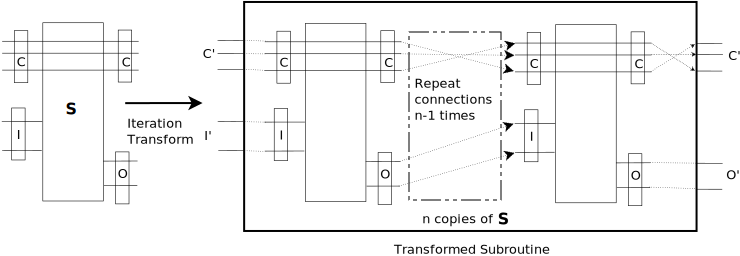
\includegraphics[scale=.4]{diagrams/SubroutineIterationTransform.png}
% \caption{Transforming a subroutine to an iterated subroutine}
% \label{fig:transforming_a_subroutine_to_an_iterated_subroutine}
\end{figure}


\end{document}
